% Options for packages loaded elsewhere
% Options for packages loaded elsewhere
\PassOptionsToPackage{unicode}{hyperref}
\PassOptionsToPackage{hyphens}{url}
%
\documentclass[
  a4paper,
]{scrbook}
\usepackage{xcolor}
\usepackage{amsmath,amssymb}
\setcounter{secnumdepth}{5}
\usepackage{iftex}
\ifPDFTeX
  \usepackage[T1]{fontenc}
  \usepackage[utf8]{inputenc}
  \usepackage{textcomp} % provide euro and other symbols
\else % if luatex or xetex
  \usepackage{unicode-math} % this also loads fontspec
  \defaultfontfeatures{Scale=MatchLowercase}
  \defaultfontfeatures[\rmfamily]{Ligatures=TeX,Scale=1}
\fi
\usepackage{lmodern}
\ifPDFTeX\else
  % xetex/luatex font selection
\fi
% Use upquote if available, for straight quotes in verbatim environments
\IfFileExists{upquote.sty}{\usepackage{upquote}}{}
\IfFileExists{microtype.sty}{% use microtype if available
  \usepackage[]{microtype}
  \UseMicrotypeSet[protrusion]{basicmath} % disable protrusion for tt fonts
}{}
\makeatletter
\@ifundefined{KOMAClassName}{% if non-KOMA class
  \IfFileExists{parskip.sty}{%
    \usepackage{parskip}
  }{% else
    \setlength{\parindent}{0pt}
    \setlength{\parskip}{6pt plus 2pt minus 1pt}}
}{% if KOMA class
  \KOMAoptions{parskip=half}}
\makeatother
% Make \paragraph and \subparagraph free-standing
\makeatletter
\ifx\paragraph\undefined\else
  \let\oldparagraph\paragraph
  \renewcommand{\paragraph}{
    \@ifstar
      \xxxParagraphStar
      \xxxParagraphNoStar
  }
  \newcommand{\xxxParagraphStar}[1]{\oldparagraph*{#1}\mbox{}}
  \newcommand{\xxxParagraphNoStar}[1]{\oldparagraph{#1}\mbox{}}
\fi
\ifx\subparagraph\undefined\else
  \let\oldsubparagraph\subparagraph
  \renewcommand{\subparagraph}{
    \@ifstar
      \xxxSubParagraphStar
      \xxxSubParagraphNoStar
  }
  \newcommand{\xxxSubParagraphStar}[1]{\oldsubparagraph*{#1}\mbox{}}
  \newcommand{\xxxSubParagraphNoStar}[1]{\oldsubparagraph{#1}\mbox{}}
\fi
\makeatother

\usepackage{color}
\usepackage{fancyvrb}
\newcommand{\VerbBar}{|}
\newcommand{\VERB}{\Verb[commandchars=\\\{\}]}
\DefineVerbatimEnvironment{Highlighting}{Verbatim}{commandchars=\\\{\}}
% Add ',fontsize=\small' for more characters per line
\usepackage{framed}
\definecolor{shadecolor}{RGB}{241,243,245}
\newenvironment{Shaded}{\begin{snugshade}}{\end{snugshade}}
\newcommand{\AlertTok}[1]{\textcolor[rgb]{0.68,0.00,0.00}{#1}}
\newcommand{\AnnotationTok}[1]{\textcolor[rgb]{0.37,0.37,0.37}{#1}}
\newcommand{\AttributeTok}[1]{\textcolor[rgb]{0.40,0.45,0.13}{#1}}
\newcommand{\BaseNTok}[1]{\textcolor[rgb]{0.68,0.00,0.00}{#1}}
\newcommand{\BuiltInTok}[1]{\textcolor[rgb]{0.00,0.23,0.31}{#1}}
\newcommand{\CharTok}[1]{\textcolor[rgb]{0.13,0.47,0.30}{#1}}
\newcommand{\CommentTok}[1]{\textcolor[rgb]{0.37,0.37,0.37}{#1}}
\newcommand{\CommentVarTok}[1]{\textcolor[rgb]{0.37,0.37,0.37}{\textit{#1}}}
\newcommand{\ConstantTok}[1]{\textcolor[rgb]{0.56,0.35,0.01}{#1}}
\newcommand{\ControlFlowTok}[1]{\textcolor[rgb]{0.00,0.23,0.31}{\textbf{#1}}}
\newcommand{\DataTypeTok}[1]{\textcolor[rgb]{0.68,0.00,0.00}{#1}}
\newcommand{\DecValTok}[1]{\textcolor[rgb]{0.68,0.00,0.00}{#1}}
\newcommand{\DocumentationTok}[1]{\textcolor[rgb]{0.37,0.37,0.37}{\textit{#1}}}
\newcommand{\ErrorTok}[1]{\textcolor[rgb]{0.68,0.00,0.00}{#1}}
\newcommand{\ExtensionTok}[1]{\textcolor[rgb]{0.00,0.23,0.31}{#1}}
\newcommand{\FloatTok}[1]{\textcolor[rgb]{0.68,0.00,0.00}{#1}}
\newcommand{\FunctionTok}[1]{\textcolor[rgb]{0.28,0.35,0.67}{#1}}
\newcommand{\ImportTok}[1]{\textcolor[rgb]{0.00,0.46,0.62}{#1}}
\newcommand{\InformationTok}[1]{\textcolor[rgb]{0.37,0.37,0.37}{#1}}
\newcommand{\KeywordTok}[1]{\textcolor[rgb]{0.00,0.23,0.31}{\textbf{#1}}}
\newcommand{\NormalTok}[1]{\textcolor[rgb]{0.00,0.23,0.31}{#1}}
\newcommand{\OperatorTok}[1]{\textcolor[rgb]{0.37,0.37,0.37}{#1}}
\newcommand{\OtherTok}[1]{\textcolor[rgb]{0.00,0.23,0.31}{#1}}
\newcommand{\PreprocessorTok}[1]{\textcolor[rgb]{0.68,0.00,0.00}{#1}}
\newcommand{\RegionMarkerTok}[1]{\textcolor[rgb]{0.00,0.23,0.31}{#1}}
\newcommand{\SpecialCharTok}[1]{\textcolor[rgb]{0.37,0.37,0.37}{#1}}
\newcommand{\SpecialStringTok}[1]{\textcolor[rgb]{0.13,0.47,0.30}{#1}}
\newcommand{\StringTok}[1]{\textcolor[rgb]{0.13,0.47,0.30}{#1}}
\newcommand{\VariableTok}[1]{\textcolor[rgb]{0.07,0.07,0.07}{#1}}
\newcommand{\VerbatimStringTok}[1]{\textcolor[rgb]{0.13,0.47,0.30}{#1}}
\newcommand{\WarningTok}[1]{\textcolor[rgb]{0.37,0.37,0.37}{\textit{#1}}}

\providecommand{\tightlist}{%
  \setlength{\itemsep}{0pt}\setlength{\parskip}{0pt}}\usepackage{longtable,booktabs,array}
\usepackage{calc} % for calculating minipage widths
% Correct order of tables after \paragraph or \subparagraph
\usepackage{etoolbox}
\makeatletter
\patchcmd\longtable{\par}{\if@noskipsec\mbox{}\fi\par}{}{}
\makeatother
% Allow footnotes in longtable head/foot
\IfFileExists{footnotehyper.sty}{\usepackage{footnotehyper}}{\usepackage{footnote}}
\makesavenoteenv{longtable}
\usepackage{graphicx}
\makeatletter
\newsavebox\pandoc@box
\newcommand*\pandocbounded[1]{% scales image to fit in text height/width
  \sbox\pandoc@box{#1}%
  \Gscale@div\@tempa{\textheight}{\dimexpr\ht\pandoc@box+\dp\pandoc@box\relax}%
  \Gscale@div\@tempb{\linewidth}{\wd\pandoc@box}%
  \ifdim\@tempb\p@<\@tempa\p@\let\@tempa\@tempb\fi% select the smaller of both
  \ifdim\@tempa\p@<\p@\scalebox{\@tempa}{\usebox\pandoc@box}%
  \else\usebox{\pandoc@box}%
  \fi%
}
% Set default figure placement to htbp
\def\fps@figure{htbp}
\makeatother
% definitions for citeproc citations
\NewDocumentCommand\citeproctext{}{}
\NewDocumentCommand\citeproc{mm}{%
  \begingroup\def\citeproctext{#2}\cite{#1}\endgroup}
\makeatletter
 % allow citations to break across lines
 \let\@cite@ofmt\@firstofone
 % avoid brackets around text for \cite:
 \def\@biblabel#1{}
 \def\@cite#1#2{{#1\if@tempswa , #2\fi}}
\makeatother
\newlength{\cslhangindent}
\setlength{\cslhangindent}{1.5em}
\newlength{\csllabelwidth}
\setlength{\csllabelwidth}{3em}
\newenvironment{CSLReferences}[2] % #1 hanging-indent, #2 entry-spacing
 {\begin{list}{}{%
  \setlength{\itemindent}{0pt}
  \setlength{\leftmargin}{0pt}
  \setlength{\parsep}{0pt}
  % turn on hanging indent if param 1 is 1
  \ifodd #1
   \setlength{\leftmargin}{\cslhangindent}
   \setlength{\itemindent}{-1\cslhangindent}
  \fi
  % set entry spacing
  \setlength{\itemsep}{#2\baselineskip}}}
 {\end{list}}
\usepackage{calc}
\newcommand{\CSLBlock}[1]{\hfill\break\parbox[t]{\linewidth}{\strut\ignorespaces#1\strut}}
\newcommand{\CSLLeftMargin}[1]{\parbox[t]{\csllabelwidth}{\strut#1\strut}}
\newcommand{\CSLRightInline}[1]{\parbox[t]{\linewidth - \csllabelwidth}{\strut#1\strut}}
\newcommand{\CSLIndent}[1]{\hspace{\cslhangindent}#1}

\usepackage{setspace}
        \let\olddescription\description
        \let\endolddescription\enddescription
        \renewenvironment{description}{
          \begin{spacing}{1.5}\olddescription
        }{
          \endolddescription\end{spacing}
        }
\usepackage{booktabs}
\usepackage{caption}
\usepackage{longtable}
\usepackage{colortbl}
\usepackage{array}
\usepackage{anyfontsize}
\usepackage{multirow}
\makeatletter
\@ifpackageloaded{bookmark}{}{\usepackage{bookmark}}
\makeatother
\makeatletter
\@ifpackageloaded{caption}{}{\usepackage{caption}}
\AtBeginDocument{%
\ifdefined\contentsname
  \renewcommand*\contentsname{Table of contents}
\else
  \newcommand\contentsname{Table of contents}
\fi
\ifdefined\listfigurename
  \renewcommand*\listfigurename{List of Figures}
\else
  \newcommand\listfigurename{List of Figures}
\fi
\ifdefined\listtablename
  \renewcommand*\listtablename{List of Tables}
\else
  \newcommand\listtablename{List of Tables}
\fi
\ifdefined\figurename
  \renewcommand*\figurename{Figure}
\else
  \newcommand\figurename{Figure}
\fi
\ifdefined\tablename
  \renewcommand*\tablename{Table}
\else
  \newcommand\tablename{Table}
\fi
}
\@ifpackageloaded{float}{}{\usepackage{float}}
\floatstyle{ruled}
\@ifundefined{c@chapter}{\newfloat{codelisting}{h}{lop}}{\newfloat{codelisting}{h}{lop}[chapter]}
\floatname{codelisting}{Listing}
\newcommand*\listoflistings{\listof{codelisting}{List of Listings}}
\makeatother
\makeatletter
\makeatother
\makeatletter
\@ifpackageloaded{caption}{}{\usepackage{caption}}
\@ifpackageloaded{subcaption}{}{\usepackage{subcaption}}
\makeatother

\usepackage{hyphenat}
\usepackage{ifthen}
\usepackage{calc}
\usepackage{calculator}



\usepackage{graphicx}
\usepackage{geometry}
\usepackage{afterpage}
\usepackage{tikz}
\usetikzlibrary{calc}
\usetikzlibrary{fadings}
\usepackage[pagecolor=none]{pagecolor}


% Set the titlepage font families







% Set the coverpage font families
\usepackage{fontspec}
\newfontfamily{\coverpagetitlefont}{QTFuture.otf}
\usepackage{fontspec}
\newfontfamily{\coverpageauthorfont}{QTFuture.otf}
\usepackage{fontspec}
\newfontfamily{\coverpagefooterfont}{QTFuture.otf}
\usepackage{fontspec}
\newfontfamily{\coverpageheaderfont}{QTFuture.otf}

\usepackage{bookmark}
\IfFileExists{xurl.sty}{\usepackage{xurl}}{} % add URL line breaks if available
\urlstyle{same}
\hypersetup{
  pdftitle={Advanced Statistical Methods and Optimization},
  pdfauthor={Prof.~Dr.~Tim Weber},
  hidelinks,
  pdfcreator={LaTeX via pandoc}}


\title{Advanced Statistical Methods and Optimization}
\author{Prof.~Dr.~Tim Weber}
\date{}
\begin{document}
%%%%% begin titlepage extension code

  \begin{frontmatter}

\begin{titlepage}
% This is a combination of Pandoc templating and LaTeX
% Pandoc templating https://pandoc.org/MANUAL.html#templates
% See the README for help

\thispagestyle{empty}

\newgeometry{top=-100in}

% Page color
\definecolor{pgcolor}{HTML}{F6D5A8}
\pagecolor{pgcolor}\afterpage{\nopagecolor}

\newcommand{\coverauthorstyle}[1]{{\fontsize{14}{16}\selectfont
\textsc{#1}}}

\begin{tikzpicture}[remember picture, overlay, inner sep=0pt, outer sep=0pt]

\tikzfading[name=fadeout, inner color=transparent!0,outer color=transparent!100]
\tikzfading[name=fadein, inner color=transparent!100,outer color=transparent!0]
\node[ scope fading=north, anchor=south west, rotate=0.0, opacity=1.0] at ($(current page.south west)+(0.0, 0.0)$) {

\includegraphics[width=\paperwidth, keepaspectratio]{img/cover.jpg}};

% Title
\newcommand{\titlelocationleft}{0.5\paperwidth}
\newcommand{\titlelocationbottom}{10.25in}
\newcommand{\titlealign}{center}

\begin{scope}{%
\fontsize{30}{36.0}\selectfont
\coverpagetitlefont
\node[anchor=north, align=center, rotate=0] (Title1) at ($(current page.south west)+(\titlelocationleft,\titlelocationbottom)$)  [text width = 0.8\paperwidth]  {{\nohyphens{Advanced
Statistical Methods and Optimization}}};
}
\end{scope}

% Author
\newcommand{\authorlocationleft}{0.5\paperwidth}
\newcommand{\authorlocationbottom}{0.5\paperheight}
\newcommand{\authoralign}{center}

\begin{scope}
{%
\fontsize{14}{16}\selectfont
\coverpageauthorfont
\node[anchor=north, align=center, rotate=0] (Author1) at ($(current page.south west)+(\authorlocationleft,\authorlocationbottom)$)  [text width = 6in]  {
\coverauthorstyle{T. A. Weber\\}};
}
\end{scope}

% Header
\newcommand{\headerlocationleft}{0.5\paperwidth}
\newcommand{\headerlocationbottom}{9in}
\newcommand{\headerlocationalign}{center}

\begin{scope}
{%
 \coverpageheaderfont
\node[anchor=north, align=center, rotate=0] (Header1) at %
($(current page.south west)+(\headerlocationleft,\headerlocationbottom)$)  [text width = 0.9\textwidth]  {{\nohyphens{Applied
AI for Digital Production Management}}};
}
\end{scope}

% Footer
\newcommand{\footerlocationleft}{0.5\paperwidth}
\newcommand{\footerlocationbottom}{0.1\textwidth}
\newcommand{\footerlocationalign}{center}

\begin{scope}
{%
\fontsize{15}{18.0}\selectfont
 \coverpagefooterfont
\node[anchor=north, align=center, rotate=0] (Footer1) at %
($(current page.south west)+(\footerlocationleft,\footerlocationbottom)$)  [text width = 0.8\paperwidth]  {{\nohyphens{Deggendorf
Institute of Technology}}};
}
\end{scope}

\end{tikzpicture}
\clearpage
\restoregeometry
\null\vfill
\begin{flushleft}
\thispagestyle{empty}
\textit{Advanced Statistical Methods and Optimzation}

© Tim A. Weber

ISBN-000000000000000

\noindent All rights reserved. No part of this publication may be produced or transmitted in any form or by any means, electronic or mechanical, including photocopying recording or any information storage and retrieval system, without the prior written permission of the publisher. For permissions contact Prof. Dr. T. Weber. Content is subject to change.
\end{flushleft}

\clearpage


\begin{center}
    \thispagestyle{empty}
    \vspace*{\fill}
    \Huge{\textit{To those who came before}}
    \vspace*{\fill}
\end{center}
\clearpage
\end{titlepage}
\setcounter{page}{1}
\end{frontmatter}

%%%%% end titlepage extension code

\renewcommand*\contentsname{Table of contents}
{
\setcounter{tocdepth}{1}
\tableofcontents
}
\listoffigures
\listoftables

\mainmatter
\bookmarksetup{startatroot}

\chapter*{Preface}\label{preface}
\addcontentsline{toc}{chapter}{Preface}

\markboth{Preface}{Preface}

This is the script for the lecture ``Advanced Statistical Methods and
Optimization'' at the DIT/Campus Cham. I do realize, that this body of
knowledge has been repeated over and over, but have decided to do my own
nonetheless so I can add my own flavor to the realms of statistics. This
work is heavily inspired by (Wickham and Grolemund 2016). Please note
that this material is copyrighted, you are not allowed to copy, at least
ask for permission - you are likely to get it.

Content is subject to change.

Tim Weber, Oct.~2024

\bookmarksetup{startatroot}

\chapter*{Glossary}\label{glossary}
\addcontentsline{toc}{chapter}{Glossary}

\markboth{Glossary}{Glossary}

\section*{List Of Acronyms}\label{acronyms_HEADER_LOA}
\addcontentsline{toc}{section}{List Of Acronyms}

\markright{List Of Acronyms}

\begin{description}
\tightlist
\item[\phantomsection\label{acronyms_ANOVA}{ANOVA}]
Analysis of Variance
\item[\phantomsection\label{acronyms_CDF}{CDF}]
Cumulative Density Function
\item[\phantomsection\label{acronyms_CI}{CI}]
Confidence Interval
\item[\phantomsection\label{acronyms_CLT}{CLT}]
Central Limit Theorem
\item[\phantomsection\label{acronyms_H0}{H0}]
Null-Hypothesis
\item[\phantomsection\label{acronyms_Ha}{Ha}]
alternative Hypothesis
\item[\phantomsection\label{acronyms_IQR}{IQR}]
Interquartile Range
\item[\phantomsection\label{acronyms_LLN}{LLN}]
Law of Large Numbers
\item[\phantomsection\label{acronyms_PDF}{PDF}]
Probability Density Function
\item[\phantomsection\label{acronyms_PMF}{PMF}]
Probability Mass Function
\item[\phantomsection\label{acronyms_PoI}{PoI}]
Parameter of Interest
\item[\phantomsection\label{acronyms_QC}{QC}]
Quality Control
\item[\phantomsection\label{acronyms_SE}{SE}]
Standard Error
\item[\phantomsection\label{acronyms_Z}{Z}]
Standard Score / Z-Score
\item[\phantomsection\label{acronyms_cl}{cl}]
confidence level
\item[\phantomsection\label{acronyms_dof}{dof}]
degree of freedom
\item[\phantomsection\label{acronyms_wrt}{wrt}]
with respect to
\end{description}

\newpage{}

\section*{Symbol Abbreviations}\label{symbol-abbreviations}
\addcontentsline{toc}{section}{Symbol Abbreviations}

\markright{Symbol Abbreviations}

\subsection*{Greek}\label{greek}
\addcontentsline{toc}{subsection}{Greek}

\begin{figure}

\begin{minipage}{0.47\linewidth}
\phantomsection\label{sign-level}{\(\alpha\)}: significance
level\end{minipage}%
%
\begin{minipage}{0.05\linewidth}
~\end{minipage}%
%
\begin{minipage}{0.47\linewidth}
\phantomsection\label{beta-risk}{\(\beta\)}: false negative risk,
\(\beta\)-risk\end{minipage}%
\newline
\begin{minipage}{0.47\linewidth}
\phantomsection\label{epsilon}{\(\epsilon\)}: residuals\end{minipage}%
%
\begin{minipage}{0.05\linewidth}
~\end{minipage}%
%
\begin{minipage}{0.47\linewidth}
\phantomsection\label{truemean-gloss}{\(\mu_0\), \(\mu\)}: the true mean
of a population\end{minipage}%
\newline
\begin{minipage}{0.47\linewidth}
\phantomsection\label{pdf-gloss}{\(\varphi(x)\)}: probability density
function\end{minipage}%
%
\begin{minipage}{0.05\linewidth}
~\end{minipage}%
%
\begin{minipage}{0.47\linewidth}
\phantomsection\label{cdf-gloss}{\(\phi(x)\)}: cumulative probability
density function or cumulative distribution function\end{minipage}%

\end{figure}%

\subsection*{Latin}\label{latin}
\addcontentsline{toc}{subsection}{Latin}

\begin{figure}

\begin{minipage}{0.47\linewidth}
\phantomsection\label{Cg}{\(C_g\)}: potential Measurement System
Capability Index\end{minipage}%
%
\begin{minipage}{0.05\linewidth}
~\end{minipage}%
%
\begin{minipage}{0.47\linewidth}
\phantomsection\label{Cgk}{\(C_{gk}\)}: Measurement Capability Index
with systematic error\end{minipage}%
\newline
\begin{minipage}{0.47\linewidth}
\phantomsection\label{Cp}{\(C_p\)}: potential process
capability\end{minipage}%
%
\begin{minipage}{0.05\linewidth}
~\end{minipage}%
%
\begin{minipage}{0.47\linewidth}
\phantomsection\label{Cpk}{\(C_{pk}\)}: actual process capability
including centering\end{minipage}%
\newline
\begin{minipage}{0.47\linewidth}
\phantomsection\label{expected-value-gloss}{\(\mathbb{E}[X]\)}: expected
value of random variable \(X\)\end{minipage}%
%
\begin{minipage}{0.05\linewidth}
~\end{minipage}%
%
\begin{minipage}{0.47\linewidth}
\phantomsection\label{numpred}{\(k\)}: number of predictors in a
model\end{minipage}%
\newline
\begin{minipage}{0.47\linewidth}
\phantomsection\label{n-gloss}{\(n\)}: number of data
points/observations in the sample\end{minipage}%
%
\begin{minipage}{0.05\linewidth}
~\end{minipage}%
%
\begin{minipage}{0.47\linewidth}
\phantomsection\label{N-gloss}{\(N\)}: number of datapoints/observations
in the population\end{minipage}%
\newline
\begin{minipage}{0.47\linewidth}
\phantomsection\label{mse}{\(MSE\)}: mean squared error\end{minipage}%
%
\begin{minipage}{0.05\linewidth}
~\end{minipage}%
%
\begin{minipage}{0.47\linewidth}
\phantomsection\label{probabilities}{\(P\)}:
Probabilities\end{minipage}%
\newline
\begin{minipage}{0.47\linewidth}
\phantomsection\label{r-gloss}{\(r\)}: range of values\end{minipage}%
%
\begin{minipage}{0.05\linewidth}
~\end{minipage}%
%
\begin{minipage}{0.47\linewidth}
\phantomsection\label{r2}{\(r^2\)}: Coefficient of
determination\end{minipage}%
\newline
\begin{minipage}{0.47\linewidth}
\phantomsection\label{r2adj}{\(r^2_{adjusted}\)}: adjusted Coefficient
of determination\end{minipage}%
%
\begin{minipage}{0.05\linewidth}
~\end{minipage}%
%
\begin{minipage}{0.47\linewidth}
\phantomsection\label{sd-gloss}{\(sd\)}: the standard deviation of a
dataset\end{minipage}%
\newline
\begin{minipage}{0.47\linewidth}
\phantomsection\label{sse}{\(SSE\)}: Sum of squared errors as calculated
by\end{minipage}%
%
\begin{minipage}{0.05\linewidth}
~\end{minipage}%
%
\begin{minipage}{0.47\linewidth}
\phantomsection\label{Var-gloss}{\(\mathrm{Var}\)}:
Variance\end{minipage}%

\end{figure}%

\newpage{}

\bookmarksetup{startatroot}

\chapter{Basic Concepts}\label{basic-concepts}

\begin{figure}[ht]

{\centering \pandocbounded{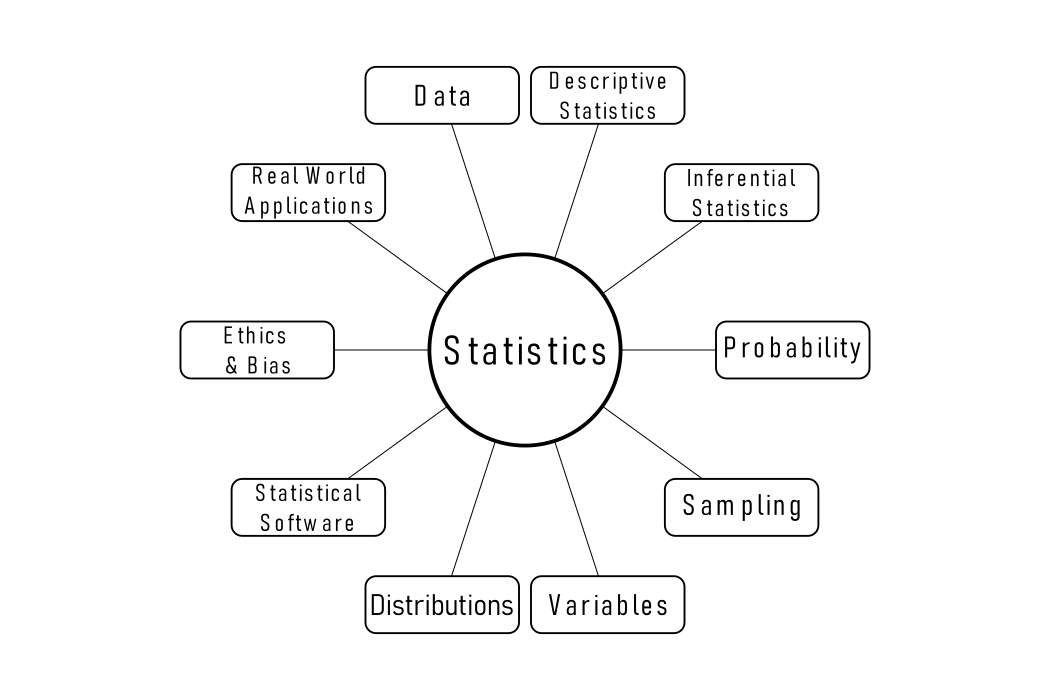
\includegraphics[keepaspectratio]{chapter000/000_basics_root.png}}

}

\caption{The necessary statistical ingredients.}

\end{figure}%

Statistics is a fundamental field that plays a crucial role in various
disciplines, from science and economics to social sciences and beyond.
It's the science of collecting, organizing, analyzing, interpreting, and
presenting data. In this introductory overview, we'll explore some key
concepts and ideas that form the foundation of statistics:

\begin{enumerate}
\def\labelenumi{\arabic{enumi}.}
\item
  \textbf{Data:} At the heart of statistics is data. Data can be
  anything from numbers and measurements to observations and information
  collected from experiments, surveys, or observations. In statistical
  analysis, we work with two main types of data: quantitative
  (numerical) and qualitative (categorical).
\item
  \textbf{Descriptive Statistics:} Descriptive statistics involve
  methods for summarizing and organizing data. These methods help us
  understand the basic characteristics of data, such as measures of
  central tendency (mean, median, mode) and measures of variability
  (range, variance, standard deviation).
\item
  \textbf{Inferential Statistics:} Inferential statistics is about
  making predictions, inferences, or decisions about a population based
  on a sample of data. This involves hypothesis testing, confidence
  intervals, and regression analysis, among other techniques.
\item
  \textbf{Probability:} Probability theory is the foundation of
  statistics. It deals with uncertainty and randomness. We use
  probability to describe the likelihood of events occurring in various
  situations, which is essential for making statistical inferences.
\item
  \textbf{Sampling:} In most cases, it's impractical to collect data
  from an entire population. Instead, we often work with samples, which
  are smaller subsets of the population. The process of selecting and
  analyzing samples is a critical aspect of statistical analysis.
\item
  \textbf{Variables:} Variables are characteristics or attributes that
  can vary from one individual or item to another. They can be
  categorized as dependent (response) or independent (predictor)
  variables, depending on their role in a statistical analysis.
\item
  \textbf{Distributions:} A probability distribution describes the
  possible values of a variable and their associated probabilities.
  Common distributions include the normal distribution, binomial
  distribution, and Poisson distribution, among others.
\item
  \textbf{Statistical Software:} In the modern era, statistical analysis
  is often conducted using specialized software packages like R, Python
  (with libraries like NumPy and Pandas), SPSS, or Excel. These tools
  facilitate data manipulation, visualization, and complex statistical
  calculations.
\item
  \textbf{Ethics and Bias:} It's essential to consider ethical
  principles in statistical analysis, including issues related to data
  privacy, confidentiality, and the potential for bias in data
  collection and interpretation.
\item
  \textbf{Real-World Applications:} Statistics has a wide range of
  applications, from medical research to marketing, finance, and social
  sciences. It helps us make informed decisions and draw meaningful
  insights from data in various fields.
\end{enumerate}

\section{Probability}\label{probability}

\subsection{Overview}\label{overview}

Probability theory is a fundamental concept in the field of statistics,
serving as the foundation upon which many statistical methods and models
are built.

\subsection{What is Probability?}\label{what-is-probability}

Probability is a mathematical concept that quantifies the uncertainty or
randomness of events. It provides a way to measure the likelihood of
different outcomes occurring in a given situation. In essence,
probability is a numerical representation of our uncertainty.

\subsection{Basic Probability
Terminology}\label{basic-probability-terminology}

\begin{itemize}
\item
  \textbf{Experiment}: An experiment is any process or procedure that
  results in an outcome. For example, rolling a fair six-sided die is an
  experiment.
\item
  \textbf{Outcome}: An outcome is a possible result of an experiment.
  When rolling a die, the outcomes are the numbers 1 through 6.
\item
  \textbf{Sample Space (S)}: The sample space is the set of all possible
  outcomes of an experiment. For a fair six-sided die, the sample space
  is \(\{1, 2, 3, 4, 5, 6\}\).
\item
  \textbf{Event (E)}: An event is a specific subset of the sample space.
  It represents a particular set of outcomes that we are interested in.
  For instance, ``rolling an even number'' is an event for a six-sided
  die, which includes outcomes \(\{2, 4, 6\}\).
\end{itemize}

\subsection{Probability Notation}\label{probability-notation}

In probability theory, we use notation to represent various concepts:

\begin{itemize}
\tightlist
\item
  \textbf{P(E)}: Probability of event E occurring.
\item
  \textbf{P(A and B)}: Probability of both events A and B occurring.
\item
  \textbf{P(A or B)}: Probability of either event A or event B
  occurring.
\item
  \textbf{P(E')}: Probability of the complement of event E, which is the
  probability of E not occurring.
\end{itemize}

\subsection{The Fundamental Principles of
Probability}\label{the-fundamental-principles-of-probability}

There are two fundamental principles of probability:

\begin{itemize}
\tightlist
\item
  \textbf{The Addition Rule}: It states that the probability of either
  event A or event B occurring is given by the sum of their individual
  probabilities, provided that the events are mutually exclusive (i.e.,
  they cannot both occur simultaneously).
\end{itemize}

\begin{align}
P(A \; or \; B) = P(A) + P(B)
\end{align}

\begin{itemize}
\tightlist
\item
  \textbf{The Multiplication Rule}: It states that the probability of
  both event A and event B occurring is the product of their individual
  probabilities, provided that the events are independent (i.e., the
  occurrence of one event does not affect the occurrence of the other).
\end{itemize}

\begin{align}
P(A \; and\;B) = P(A) * P(B)
\end{align}

\subsection{Example: Rolling a Fair Six-Sided
Die}\label{example-rolling-a-fair-six-sided-die}

Consider rolling a fair six-sided die.

\begin{itemize}
\tightlist
\item
  Sample Space (S): \(\{1, 2, 3, 4, 5, 6\}\) (Figure~\ref{fig-prob})
\item
  Event A: Rolling an even number = \(\{2, 4, 6\}\)
  (Figure~\ref{fig-prob})
\item
  Event B: Rolling a number greater than \(3 = \{4, 5, 6\}\)
  (Figure~\ref{fig-prob})
\end{itemize}

\begin{figure}[ht]

\centering{

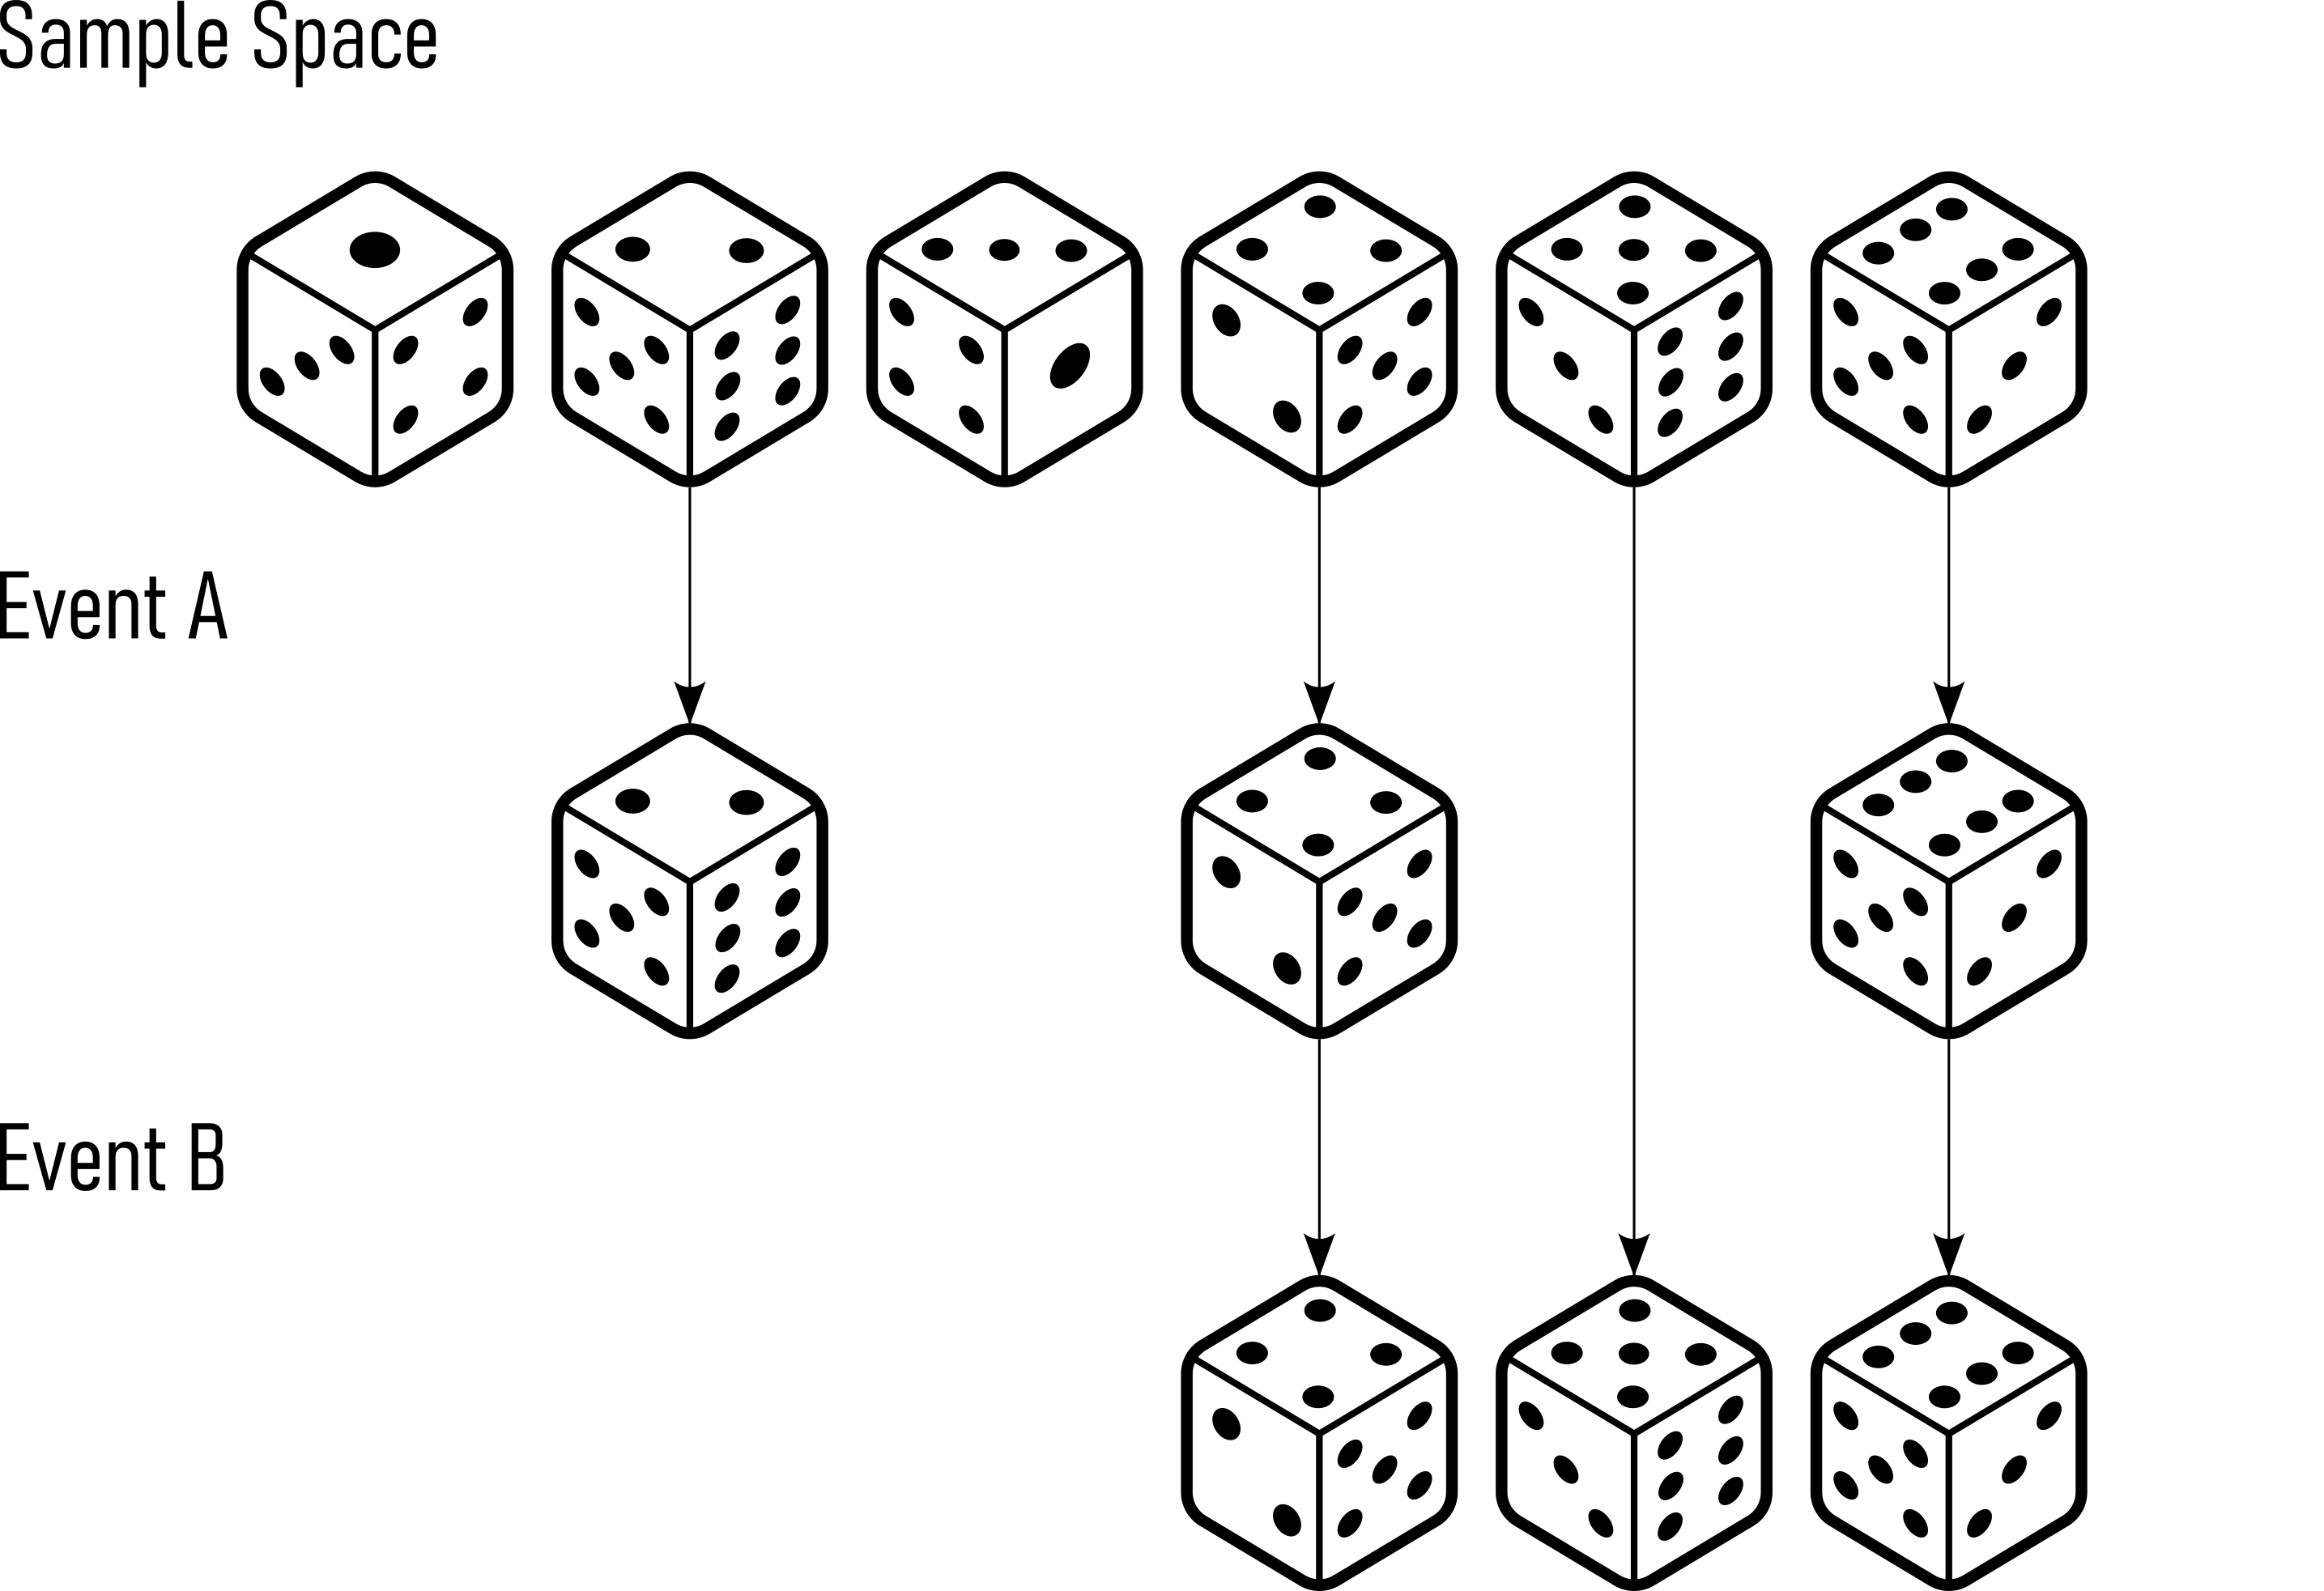
\includegraphics[width=0.75\linewidth,height=\textheight,keepaspectratio]{chapter000/010_Probability.png}

}

\caption{\label{fig-prob}This example's sample space, as well as event A
and event B.}

\end{figure}%

\subsection{Probability in action - The Galton
Board}\label{probability-in-action---the-galton-board}

A Galton board, also known as a bean machine or a quincunx, is a
mechanical device that demonstrates the principles of probability and
the normal distribution. It was invented by Sir Francis
Galton\footnote{Sir Francis Galton (1822-1911): Influential English
  scientist, notable for his contributions to statistics and genetics.}
in the late 19th century. The Galton board consists of a vertical board
with a series of pegs or nails arranged in triangular or hexagonal
patterns.

A Galton board, also known as a bean machine or a quincunx, is a
mechanical device that demonstrates the principles of probability and
the normal distribution. It was invented by Sir Francis Galton in the
late 19th century. The Galton board consists of a vertical board with a
series of pegs or nails arranged in triangular or hexagonal patterns.

\begin{enumerate}
\def\labelenumi{\arabic{enumi}.}
\item
  \textbf{Initial Release}: At the top of the Galton board, a ball or
  particle is released. This ball can take one of two paths at each peg,
  either to the left or to the right. The decision at each peg is
  determined by chance, such as the flip of a coin or the roll of a die.
  This represents a random event.
\item
  \textbf{Multiple Trials}: As the ball progresses downward, it
  encounters several pegs, each of which randomly directs it either left
  or right. The ball continues to bounce off pegs until it reaches the
  bottom.
\item
  \textbf{Accumulation}: Over multiple trials or runs of the Galton
  board, you will notice that the balls accumulate in a pattern at the
  bottom. This pattern forms a bell-shaped curve, which is the hallmark
  of a normal distribution.
\item
  \textbf{Normal Distribution}: The accumulation of balls at the bottom
  resembles the shape of a normal distribution curve. This means that
  the majority of balls will tend to accumulate in the center, forming
  the peak of the curve, while fewer balls will accumulate at the
  extreme left and right sides.
\end{enumerate}

The Galton board is a visual representation of the
\hyperref[clt]{central limit theorem}, a fundamental concept in
probability theory. It demonstrates how random events, when repeated
many times, tend to follow a normal distribution. This distribution is
commonly observed in various natural phenomena and is essential in
statistical analysis.

\begin{figure}[ht]

\centering{

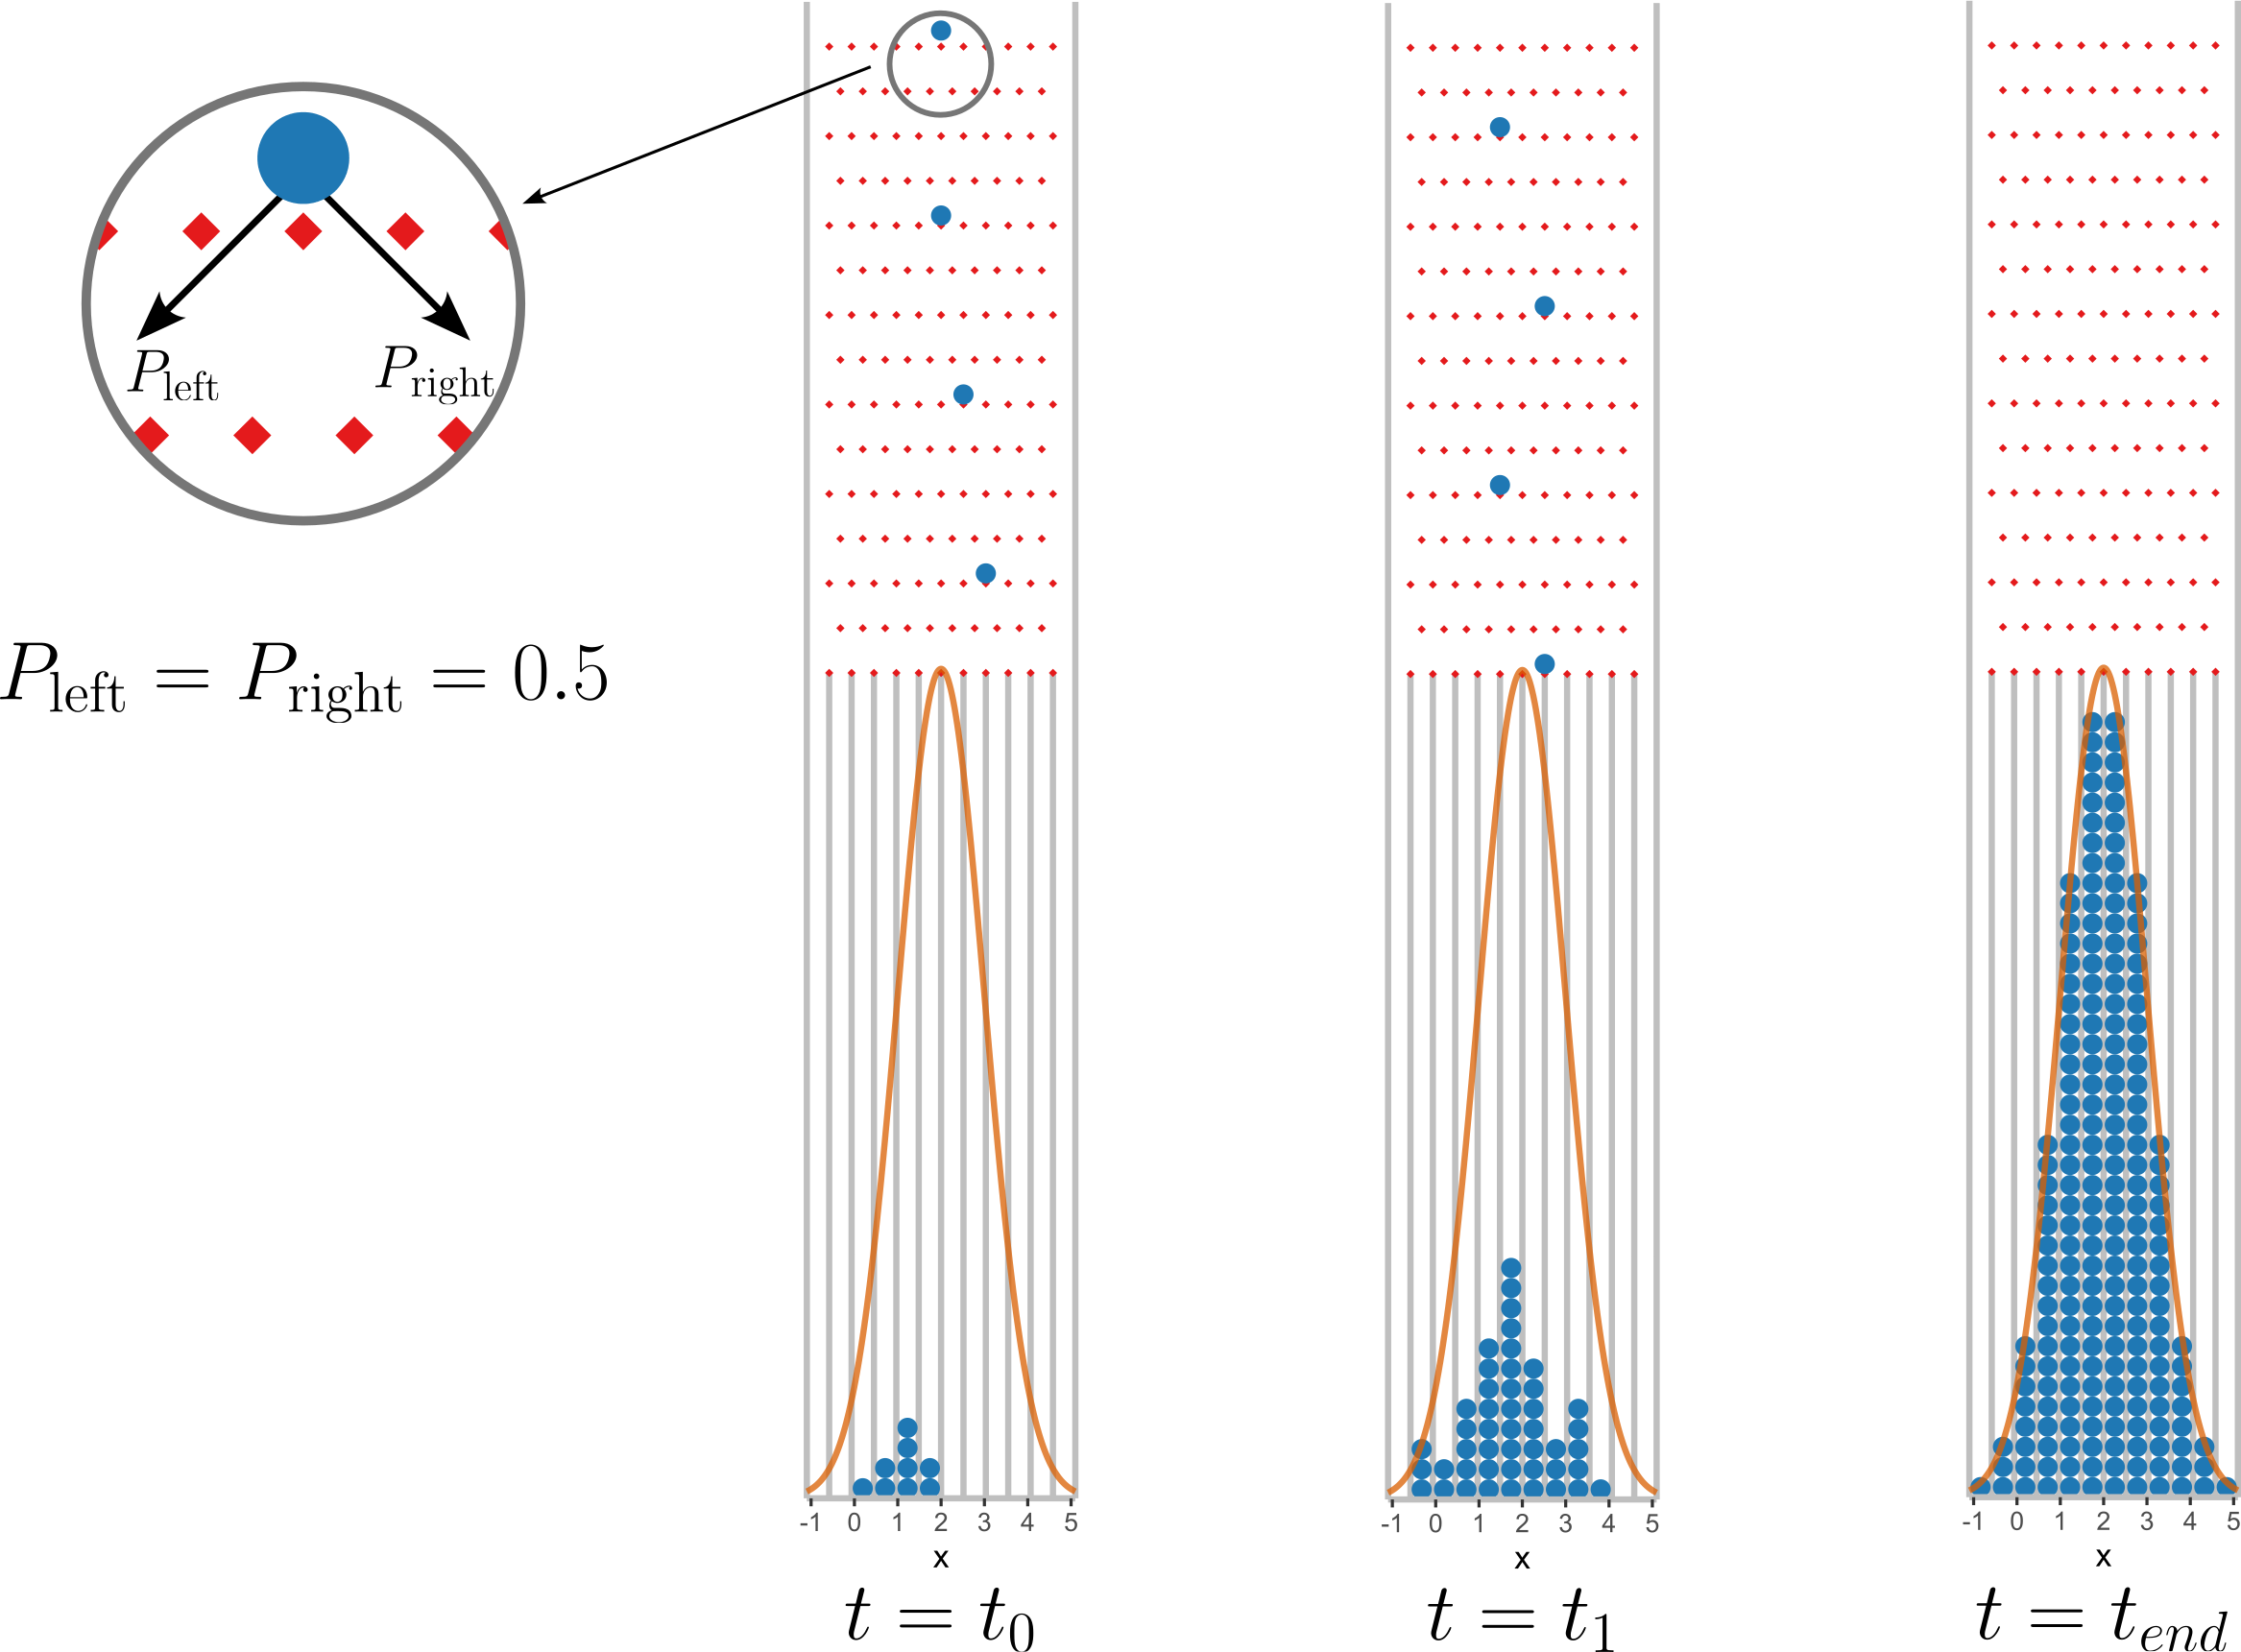
\includegraphics[width=0.75\linewidth,height=\textheight,keepaspectratio]{chapter000/011_Plinko.png}

}

\caption{\label{fig-plinko}A Galton board in action.}

\end{figure}%

\subsubsection{Statistics and
Probabbility}\label{statistics-and-probabbility}

The Galton board is a nice example how statistics emerge from
probability.

\paragraph{Define the problem}\label{define-the-problem}

\begin{itemize}
\tightlist
\item
  The board has \(n\) rows of pegs (columns)
\item
  Each ball has an equal probability of moving left or right (assuming
  no bias)
\item
  The number of rightward moves determines the final position in the
  bins
\end{itemize}

\paragraph{Step 2: Binomial Probability
Distribution}\label{step-2-binomial-probability-distribution}

Each ball independently moves right (\(R\)) or left (\(L\)) with a
probability of \(p=0.5\).

The number of rightwards moves follows a binomial distribution.

\begin{align}
P(k) = \binom{n}{k} p^k (1 - p)^{n - k} 
\end{align}

\begin{description}
\tightlist
\item[\(n\)]
total number of columns (or pegs encountered)
\item[\(k\)]
number of rightward moves
\item[\(\binom{n}{k}\)]
biomial coefficient, given by \(\binom{n}{k} = \frac{n!}{k!(n-k)!}\)
\end{description}

with \(p = 0.5\) this simplifies to

\begin{align}
P(k) = \binom{n}{k} ( \frac{1}{2})^n
\end{align}

\paragraph{Step 3: Position Mapping}\label{step-3-position-mapping}

The final position of a ball in a bin corresponds to the number of
rightwards moves \(k\). If the bins are indexed from \(0\) to \(n\)
(where \(k=0\) means all left moves and \(k=n\) means all right moves)
the probability of landing in bin \(k\) is:

\begin{align}
P(k) = \frac{n!}{k!(n-k)!}(\frac{1}{2})^n
\end{align}

\section{\texorpdfstring{\hyperref[acronyms_CLT]{Central Limit Theorem
(CLT)}}{Central Limit Theorem (CLT)}}\label{section}

\begin{figure}[ht]

\centering{

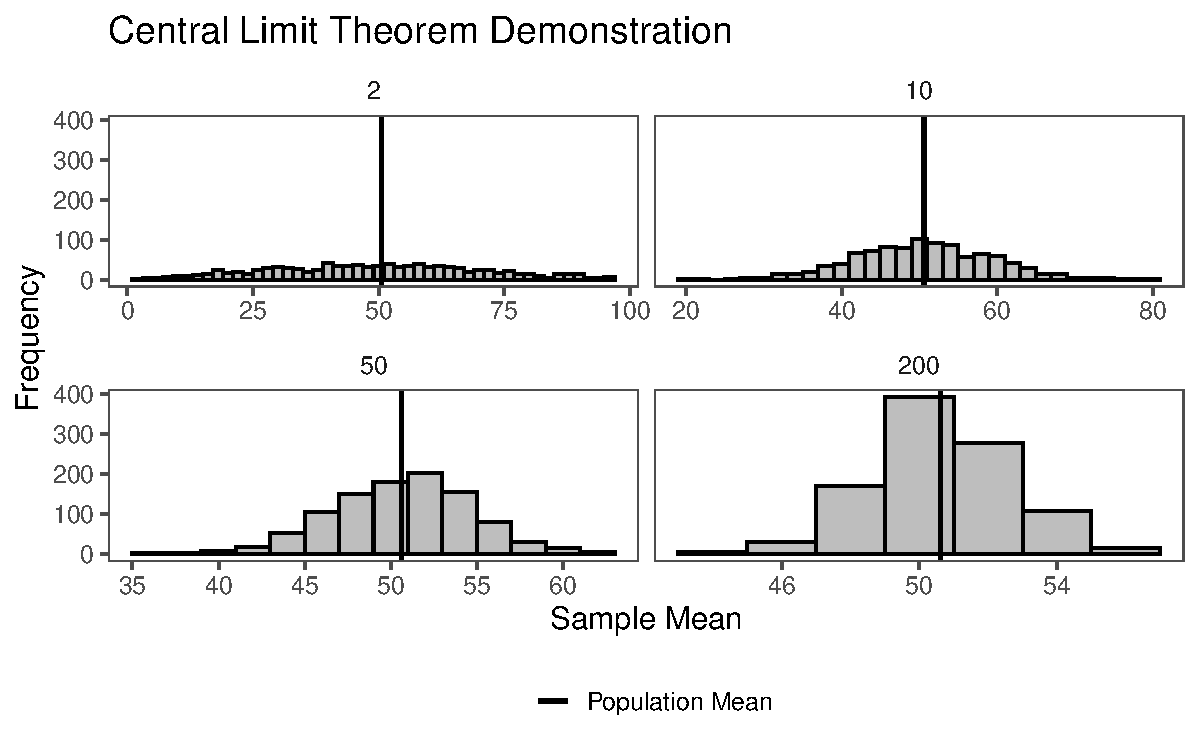
\includegraphics[width=0.99\linewidth,height=\textheight,keepaspectratio]{chapter000_BasicConcepts_files/figure-pdf/fig-clt-1.pdf}

}

\caption{\label{fig-clt}The central limit theorem in action.}

\end{figure}%

The primary reason for the existence of the normal distribution in many
real-world datasets is the \hyperref[acronyms_CLT]{CLT} (Taboga 2017).
The \hyperref[acronyms_CLT]{CLT} states that when you take a large
enough number of random samples from any population, the distribution of
the sample means will tend to follow a normal distribution, even if the
original population distribution is not normal. This means that the
normal distribution emerges as a statistical consequence of aggregating
random data points. This is shown in Figure~\ref{fig-clt}.

From \(n=10000\) uniformly distributed data points (the
\emph{population}) (\(min=1, max = 100\)) either \(2,10,50\) or \(200\)
samples are taken randomly (the \emph{samples}). For each of the samples
the mean is calculated, resulting in \(1000\) mean values for each
(\(2,10,50\) or \(200\)) sample size. In Figure~\ref{fig-clt} the
results from this numerical study are shown. The larger the sample size,
the closer the mean calculated \hyperref[mean-gloss]{\(\bar{x}\)}is to
the population mean (\hyperref[truemean-gloss]{\(\mu_0\)}). The effect
is especially large on the standard deviation, resulting in a smaller
standard deviation the larger the sample size is.

\section{\texorpdfstring{\hyperref[acronyms_LLN]{Law of Large Numbers
(LLN)}}{Law of Large Numbers (LLN)}}\label{section-1}

\begin{figure}[H]

\centering{

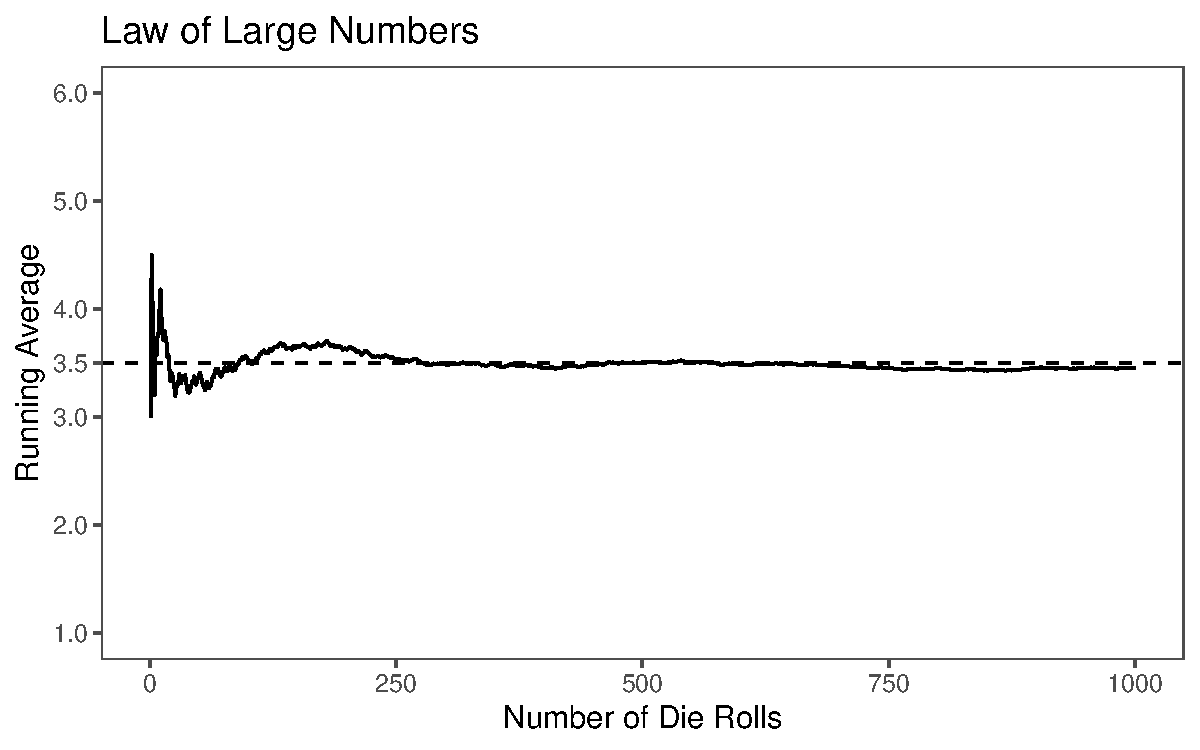
\includegraphics[width=0.75\linewidth,height=\textheight,keepaspectratio]{chapter000_BasicConcepts_files/figure-pdf/fig-lln-1.pdf}

}

\caption{\label{fig-lln}The Law of Large Numbers in Action with die
rolls as an example.}

\end{figure}%

The \hyperref[acronyms_CLT]{CLT} states that as the size of a random
sample increases, the sample average converges to the population mean.
This law, along with the \hyperref[acronyms_CLT]{CLT}, explains why the
normal distribution frequently arises. When you take many small,
independent, and identically distributed measurements and compute their
averages, these averages tend to cluster around the true population
mean, forming a normal distribution Johnson (1994).

The \hyperref[lln]{LLN} ar work is shown in Figure~\ref{fig-lln}. A fair
six-sided die is rolled 1000 times and the running average of the roll
results after each roll is calculated. The resulting line plot shows how
the running average approaches the expected value of \(3.5\), which is
the average of all possible outcomes of the die. The line in the plot
represents the running average It fluctuates at the beginning but
gradually converges toward the expected value of \(3.5\). To emphasize
this convergence, a dashed line indicating the theoretical expected
value which is essentially the expected value applied to each roll. This
visualization demonstrates the Law of Large Numbers, which states that
as the number of trials or rolls increases, the \emph{sample mean}
(running average in this case) approaches the \emph{population mean}
(expected value) with greater accuracy, showing the predictability and
stability of random processes over a large number of observations.

\section{Population}\label{population}

\begin{figure}[ht]

{\centering 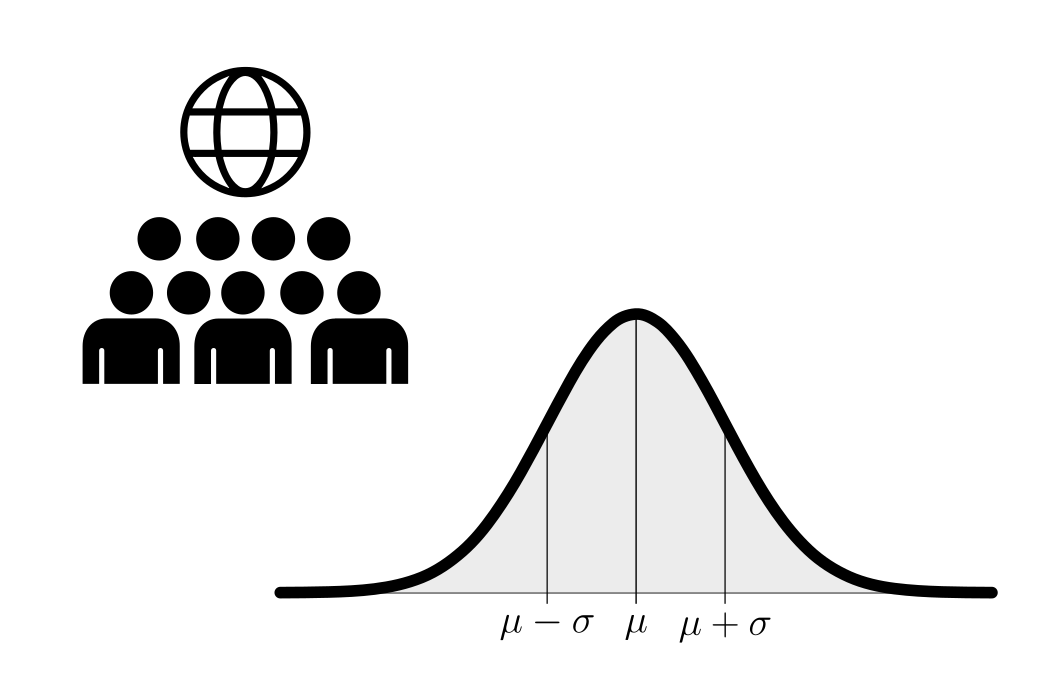
\includegraphics[width=0.75\linewidth,height=\textheight,keepaspectratio]{chapter000/002_Population.png}

}

\caption{An example for a population.}

\end{figure}%

In statistics, a population is the complete set of individuals, items,
or data points that are the subject of a study. Understanding
populations and how to work with them is fundamental in statistical
analysis, as it forms the basis for making meaningful inferences and
drawing conclusions about the broader group being studied. It is the
complete collection of all elements that share a common characteristic
or feature and is of interest to the researcher. The population can vary
widely depending on the research question or problem at hand. A
populations \emph{true mean} is depicted with
\hyperref[truemean-gloss]{\(\mu_0\)} and the variance is depicted with
\hyperref[truevariance-gloss]{\(\sigma_0^2\)}.

\section{Sample}\label{sample}

\begin{figure}[ht]

{\centering 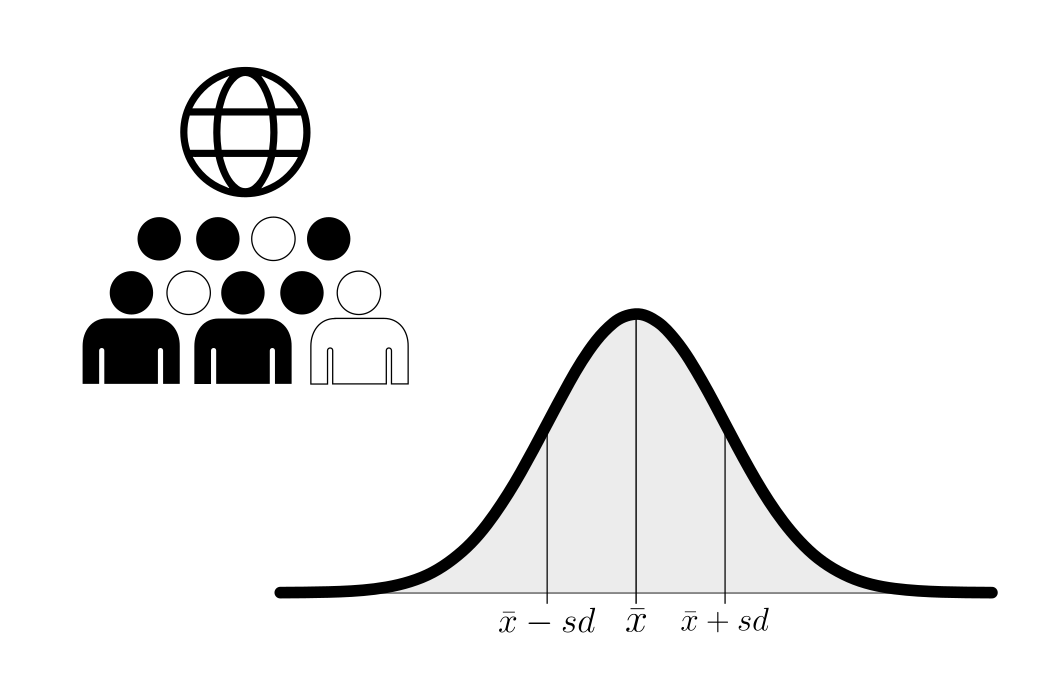
\includegraphics[width=0.75\linewidth,height=\textheight,keepaspectratio]{chapter000/003_Sample.png}

}

\caption{A sample drawn from the population.}

\end{figure}%

The key principles behind a sample include its role as a manageable
subset of data, which can be chosen randomly or purposefully. Ideally,
it should be representative, reflecting the characteristics and
diversity of the larger population. Statistical techniques are then
applied to this sample to make inferences, estimate population
parameters, or test hypotheses. The size of the sample matters, as a
larger sample often leads to more precise estimates, but it should be
determined based on research goals and available resources. Various
sampling methods, such as random sampling, stratified sampling, or
cluster sampling, can be employed depending on the research objectives
and population characteristics. A samples \emph{true mean} is depicted
with \hyperref[mean-gloss]{\(\bar{x}\)} and the variance is depicted
with \hyperref[sd-gloss]{\(sd\)}.

\section{Descriptive Statistics}\label{descriptive-statistics}

Descriptive statistics are used to summarize and describe the main
features of a data set. They provide a way to organize, present, and
analyze data in a meaningful and concise manner. Descriptive statistics
do not involve making inferences or drawing conclusions beyond the data
that is being analyzed. Instead, they aim to provide a clear and
accurate representation of the data set. Some common techniques and
measures used in descriptive statistics include:

\subsection{Example Data: The drive shaft
exercise}\label{example-data-the-drive-shaft-exercise}

\begin{figure}[ht]

\centering{

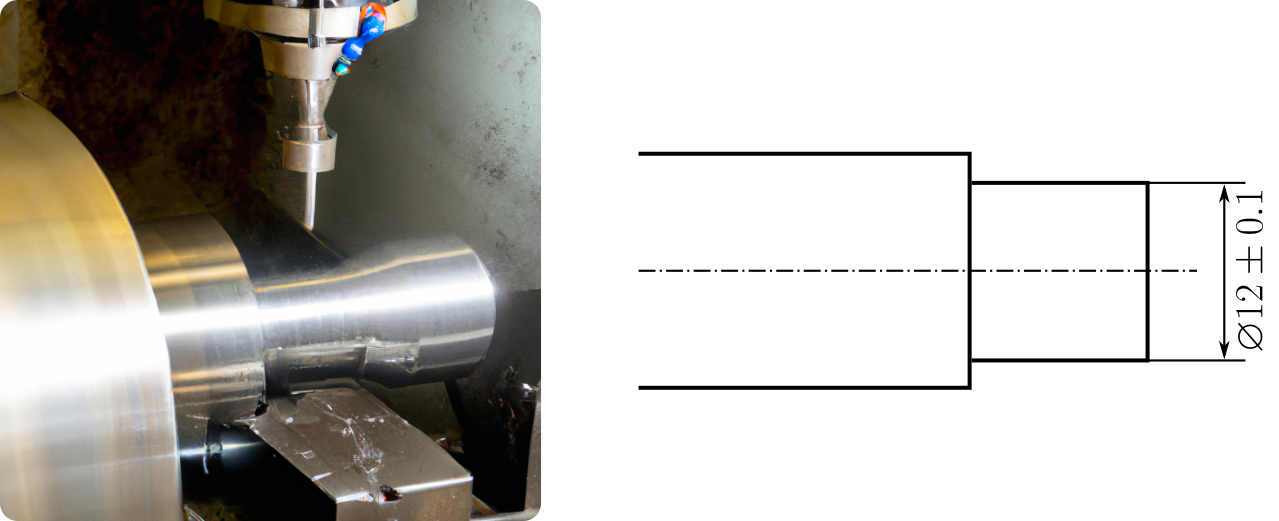
\includegraphics[width=0.75\linewidth,height=\textheight,keepaspectratio]{chapter000/005_DriveShaft.png}

}

\caption{\label{fig-drive-shaft-intro}The drive shaft specification.}

\end{figure}%

\begin{figure}[ht]

\centering{

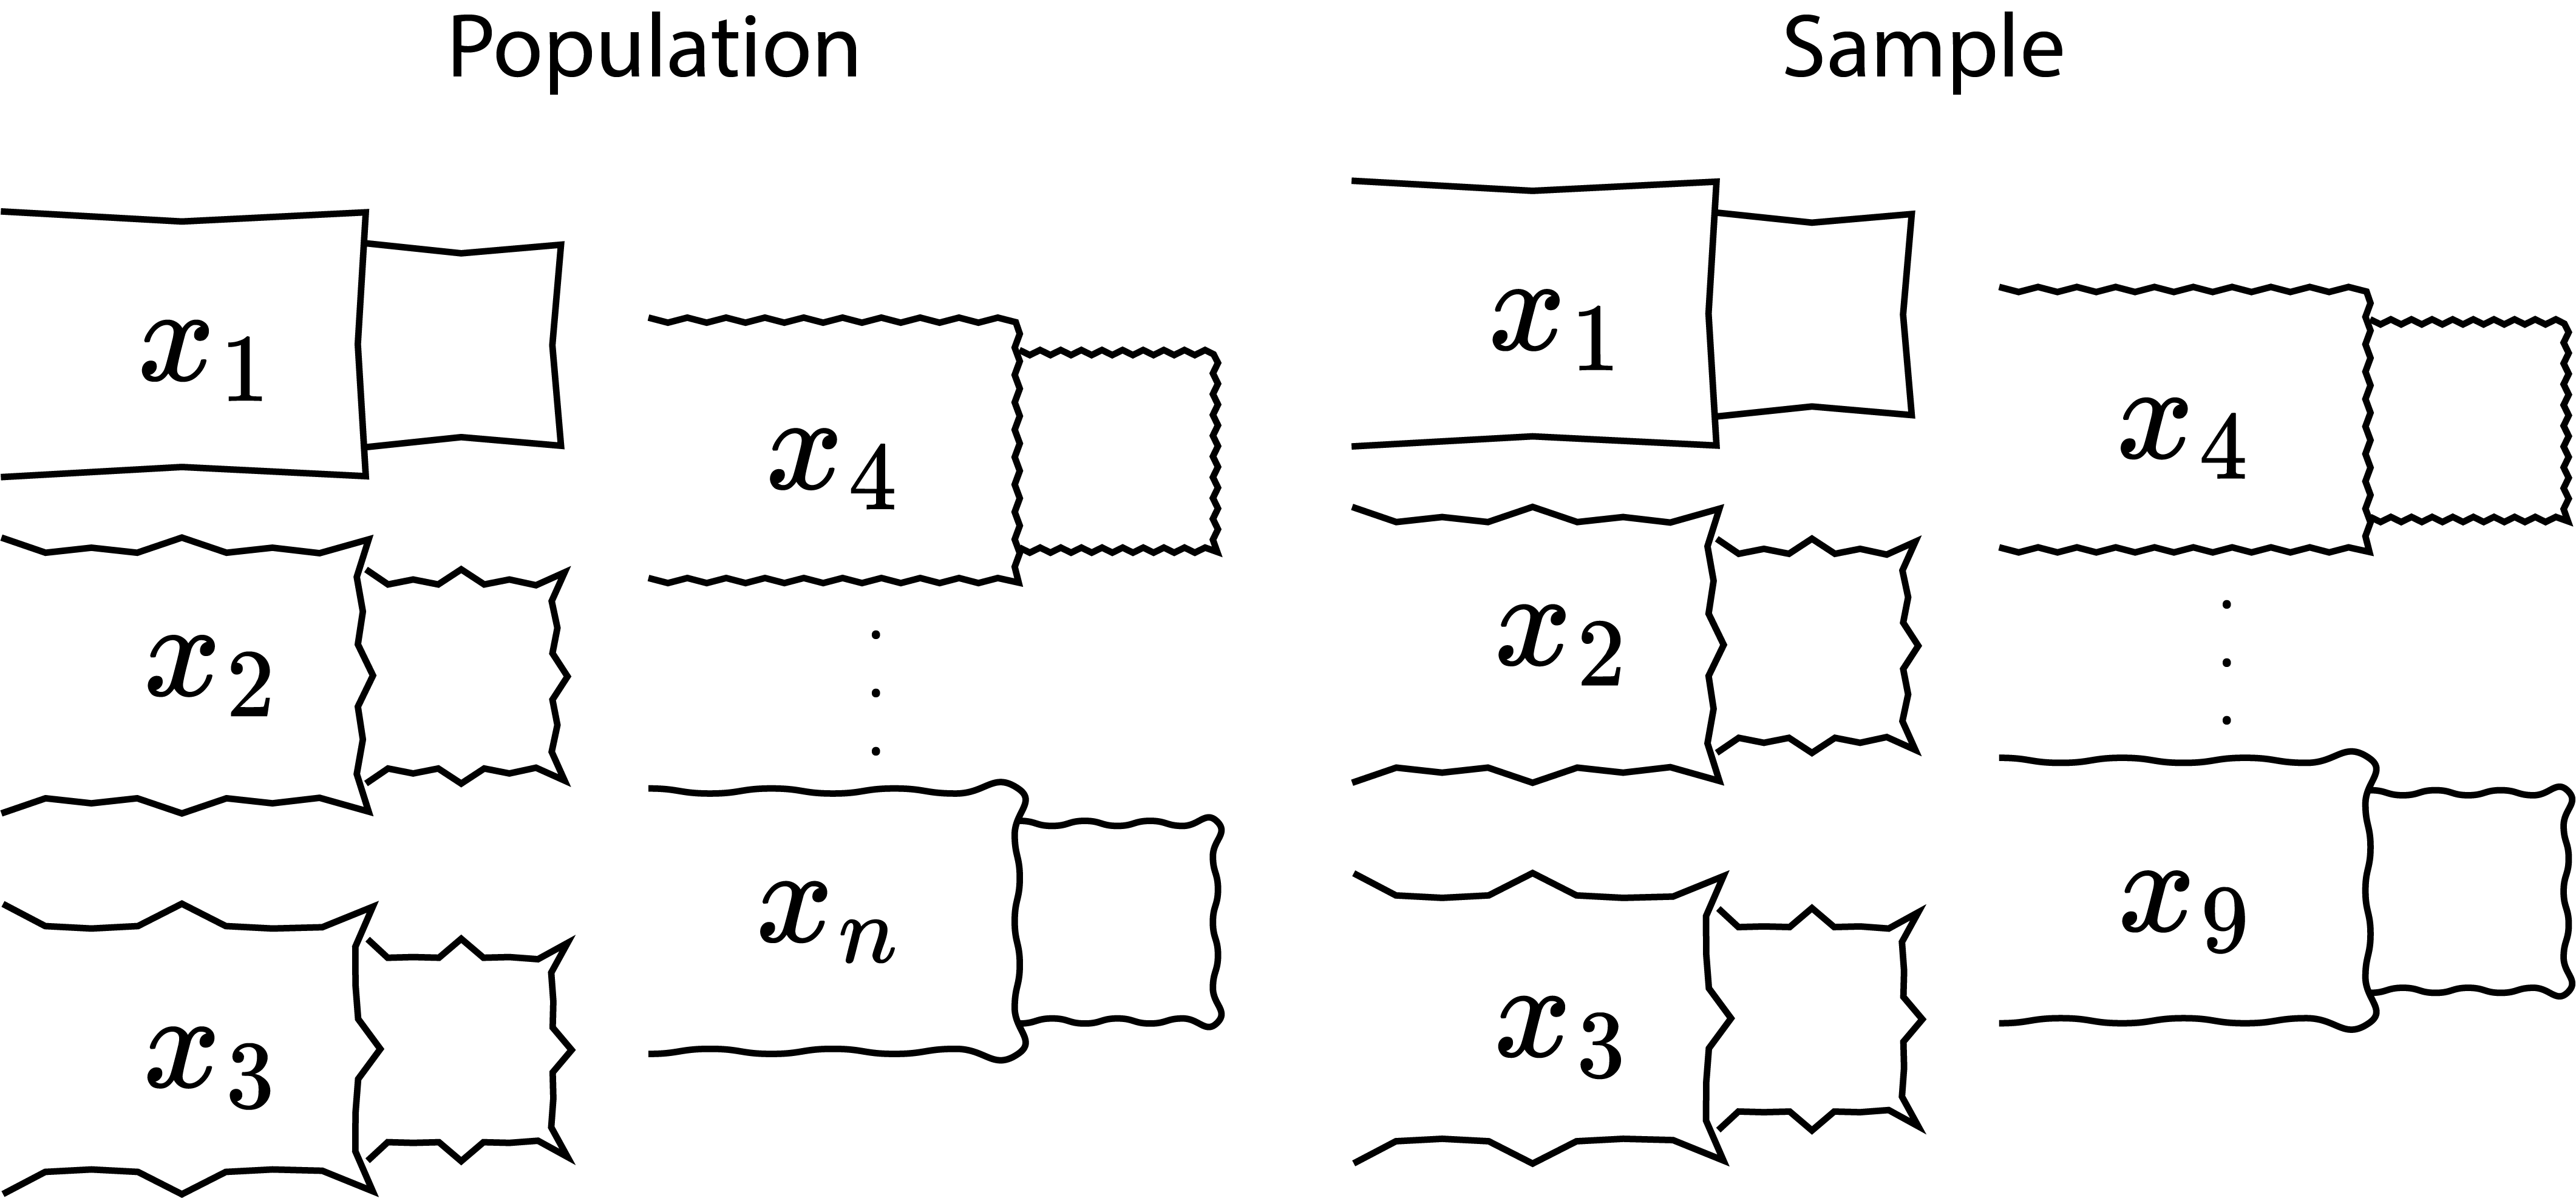
\includegraphics[width=0.95\linewidth,height=\textheight,keepaspectratio]{chapter000/DriveShaft_Intro.png}

}

\caption{\label{fig-drive-shaft-pop-smpl}Difference between the
population of ALL drive shafts and a sample of drive shafts.}

\end{figure}%

\subsection{Measures of Central
Tendency}\label{measures-of-central-tendency}

Measures of central tendency are essential in statistics because they
provide a single value that summarizes or represents the center point or
typical value of a dataset. The main reasons for using these measures
include:

\begin{itemize}
\item
  Simplification of Data: They condense large sets of data into a single
  representative value, making the data easier to understand and
  interpret.
\item
  Comparison Across Datasets: They allow for straightforward comparison
  between different groups or datasets by providing a common reference
  point.
\item
  Foundation for Further Analysis: Many statistical techniques and
  models rely on an understanding of central tendency as a starting
  point, such as in regression analysis or hypothesis testing.
\item
  Decision-Making: In fields such as economics, education, and public
  policy, central tendency helps inform decisions based on typical
  outcomes or behaviors (e.g., average income, median test scores).
\item
  Identification of Patterns: They help identify patterns and trends
  over time, especially in time-series data or longitudinal studies.
\end{itemize}

\begin{figure}[ht]

\centering{

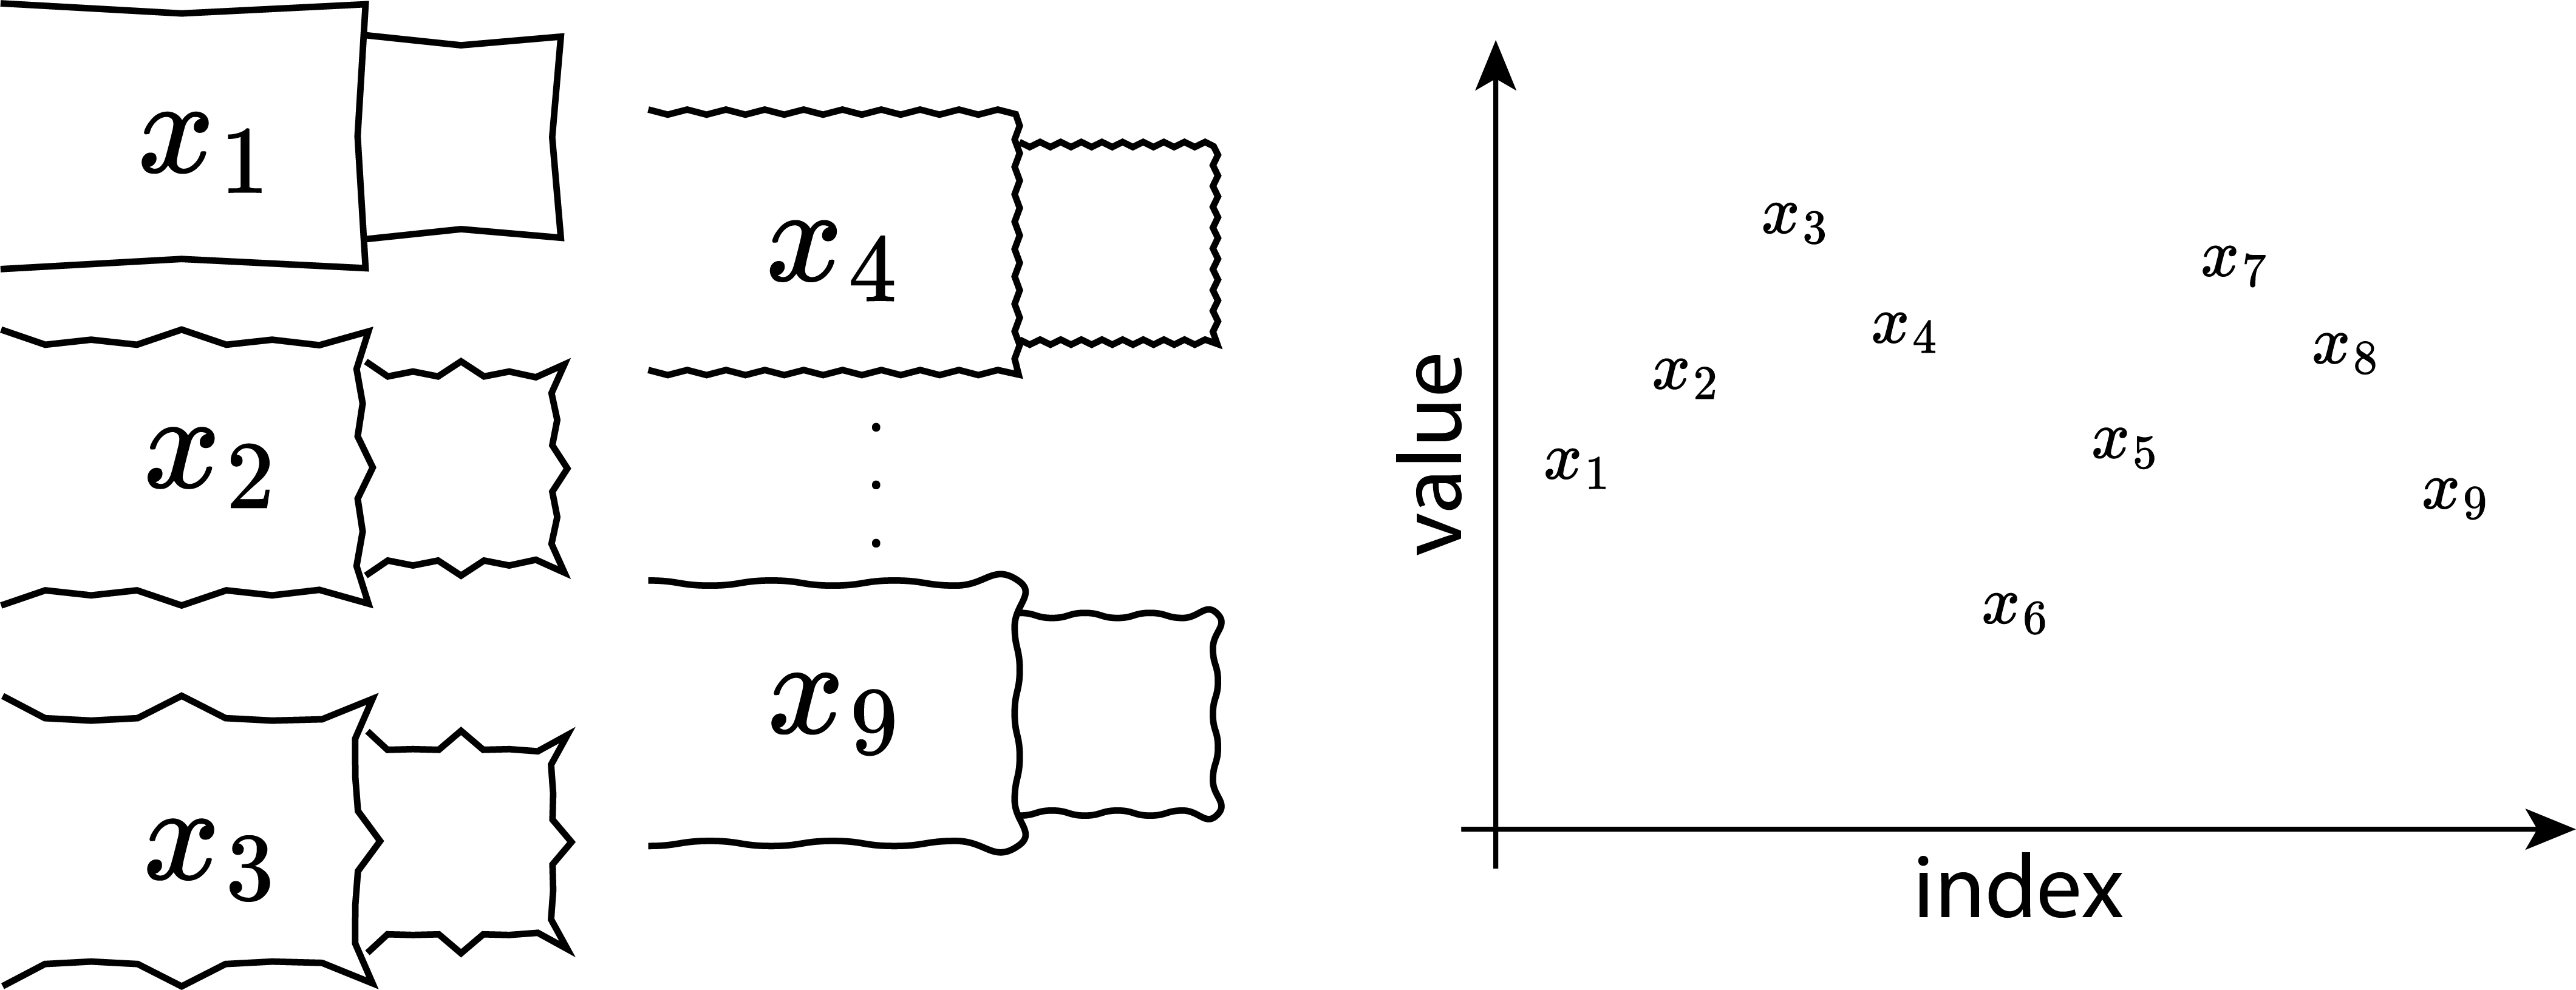
\includegraphics[width=0.95\linewidth,height=\textheight,keepaspectratio]{chapter000/DriveShaft_central_tendency.png}

}

\caption{\label{fig-dat}Some drive shaft sample data in a 2D plot of
sample index vs.~variable value}

\end{figure}%

\begin{figure}[ht]

\centering{

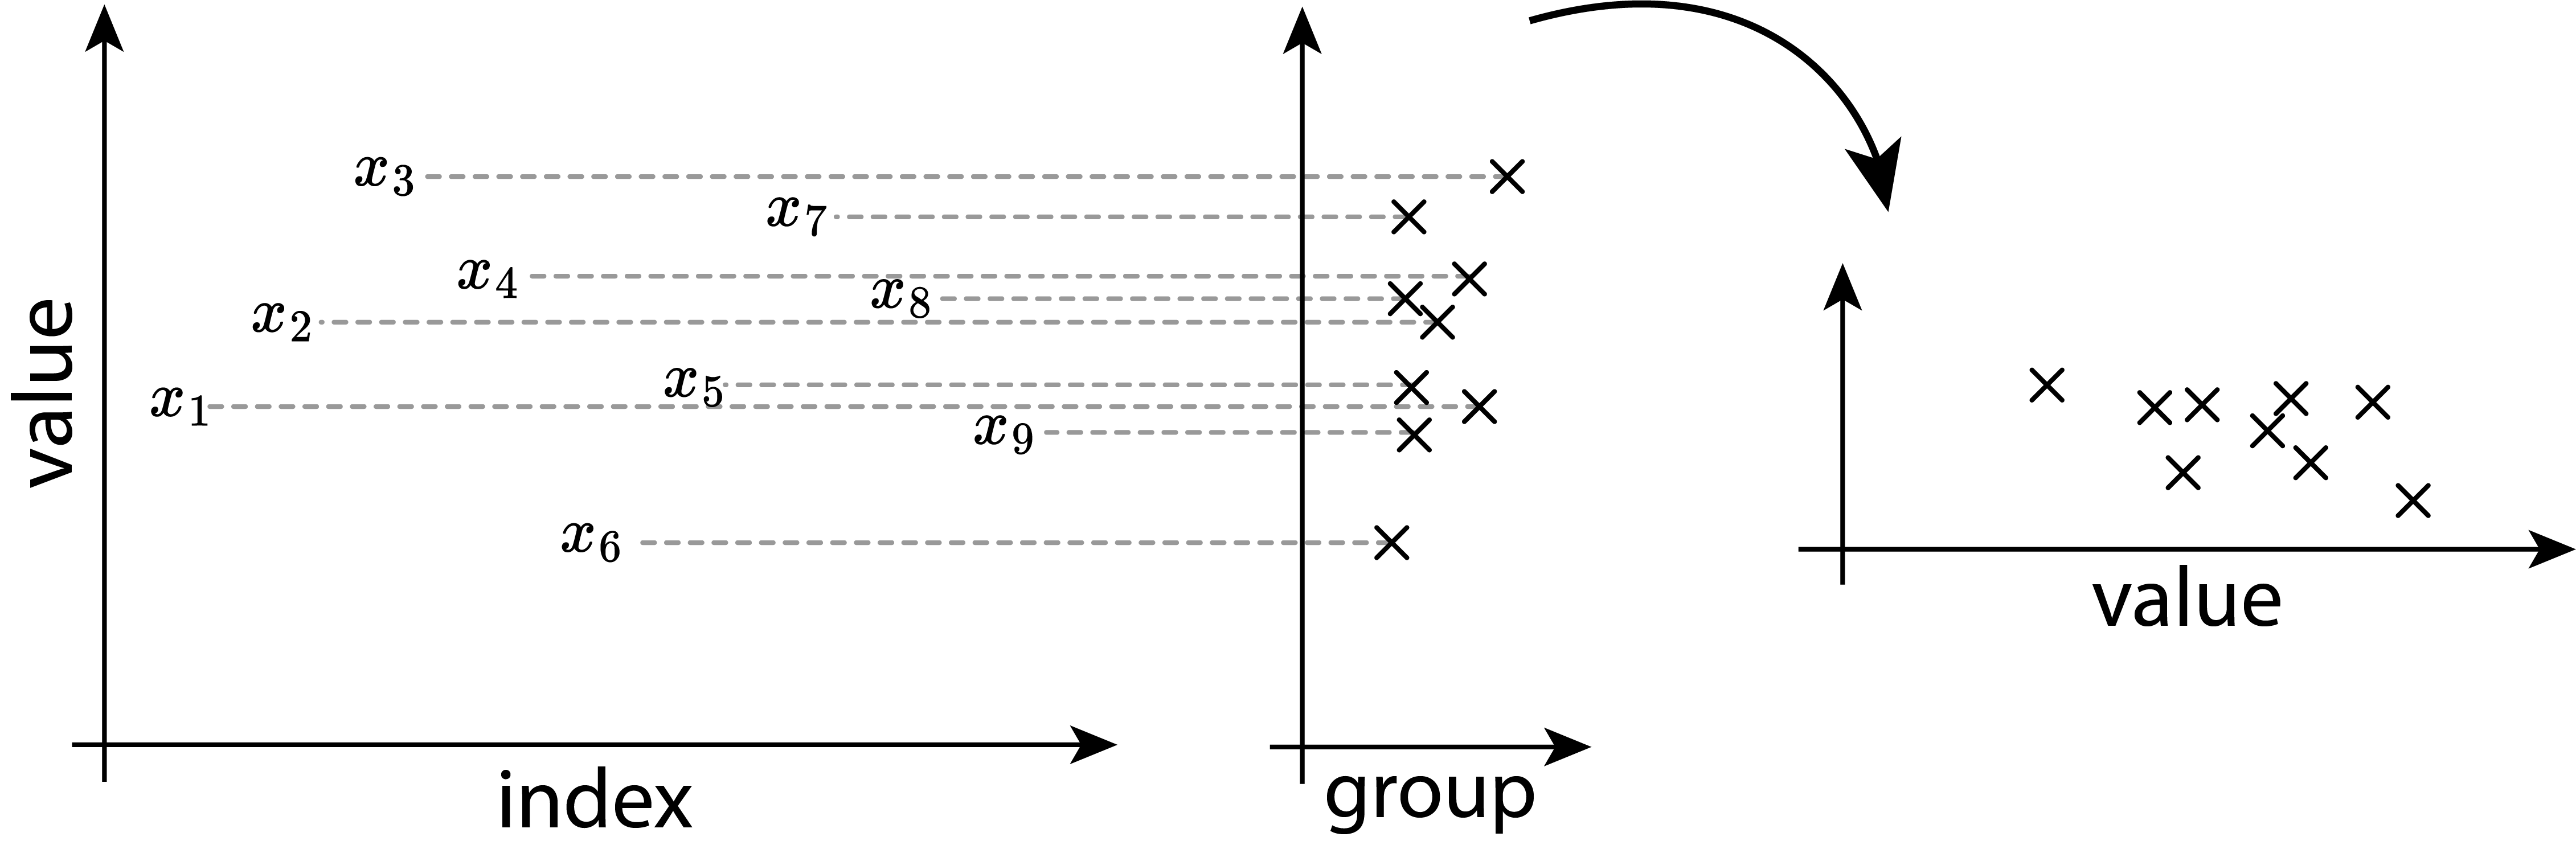
\includegraphics[width=0.95\linewidth,height=\textheight,keepaspectratio]{chapter000/DriveShaft_ct_data.png}

}

\caption{\label{fig-central-tend}Some drive shaft sample data in a 2D
plot of sample index vs.~variable value}

\end{figure}%

\subsubsection{Mean}\label{mean}

\begin{figure}[ht]

\centering{

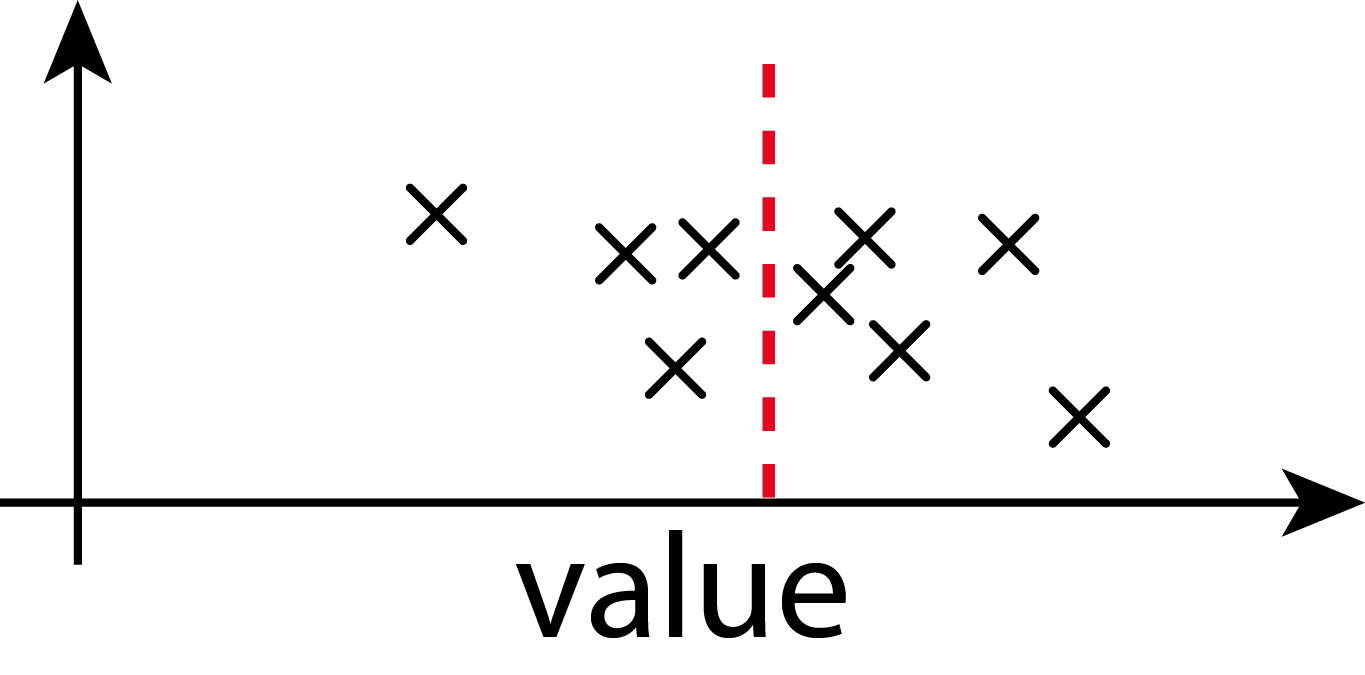
\includegraphics[width=0.5\linewidth,height=\textheight,keepaspectratio]{chapter000/mean_ds.png}

}

\caption{\label{fig-mean-ds}A graphical depiction of the mean}

\end{figure}%

\begin{align}
\text{discrete: } \mu = \mathbb{E}[X] &= \sum_{i=1}^{n} x_i \, p_i \\
\text{continous: }\mu = \mathbb{E}[X] &= \int_{-\infty}^{\infty} x \, f(x) \, dx
\end{align}

\begin{align}
\text{population:} \; \mu &= \frac{1}{N}\sum_i^{N} x_i \\
\text{sample:} \; \bar{x} &= \frac{1}{n}\sum_i^{n} x_i 
\end{align}

\subsubsection{Median}\label{median}

\begin{figure}[ht]

\centering{

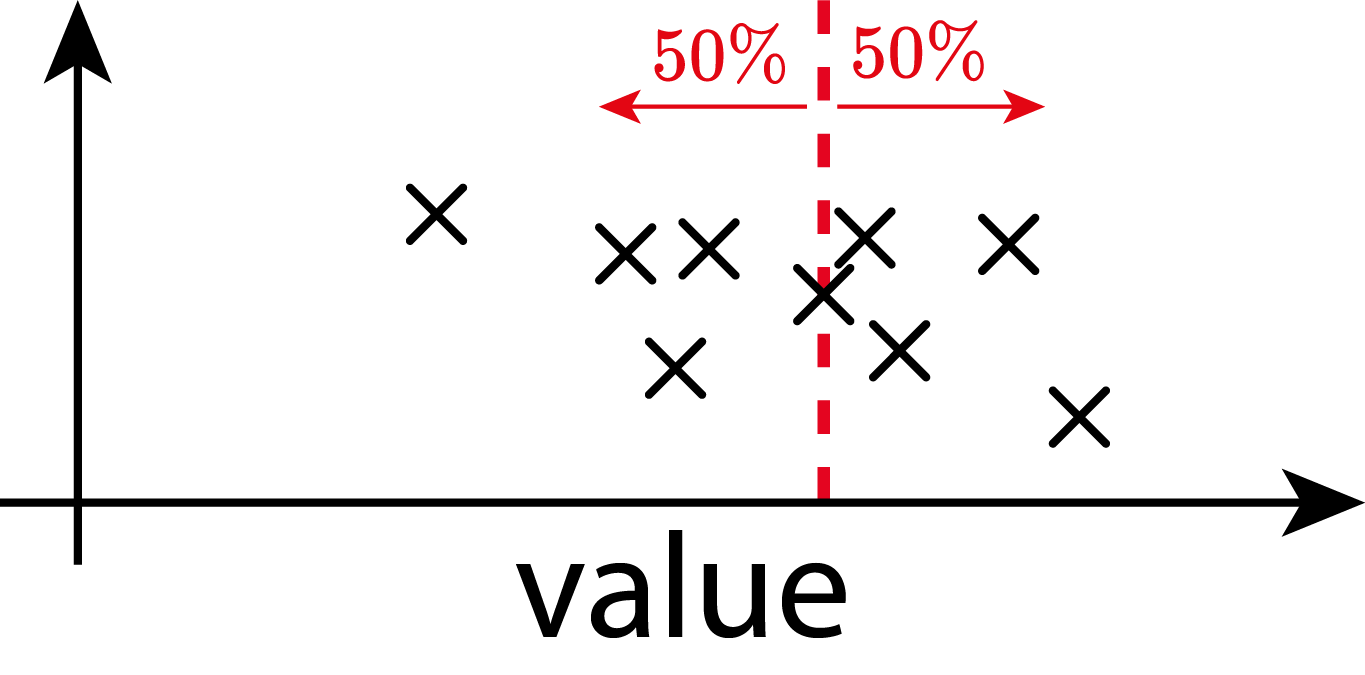
\includegraphics[width=0.95\linewidth,height=\textheight,keepaspectratio]{chapter000/median_ds.png}

}

\caption{\label{fig-median-ds}A graphical depiction of the median}

\end{figure}%

\begin{align}
\text{population:} \; m &= 
\begin{cases}
x_{\left(\frac{N+1}{2}\right)} & \text{if } N \text{ is odd} \\
\frac{1}{2} \left( x_{\left(\frac{N}{2}\right)} + x_{\left(\frac{N}{2} + 1\right)} \right) & \text{if } N \text{ is even}
\end{cases} \\ 
\text{sample:} \; \tilde{x} &= 
\begin{cases}
x_{\left(\frac{n+1}{2}\right)} & \text{if } n \text{ is odd} \\
\frac{1}{2} \left( x_{\left(\frac{n}{2}\right)} + x_{\left(\frac{n}{2} + 1\right)} \right) & \text{if } n \text{ is even}
\end{cases} 
\end{align}

\subsection{Measures of Spread}\label{measures-of-spread}

\begin{figure}[ht]

\centering{

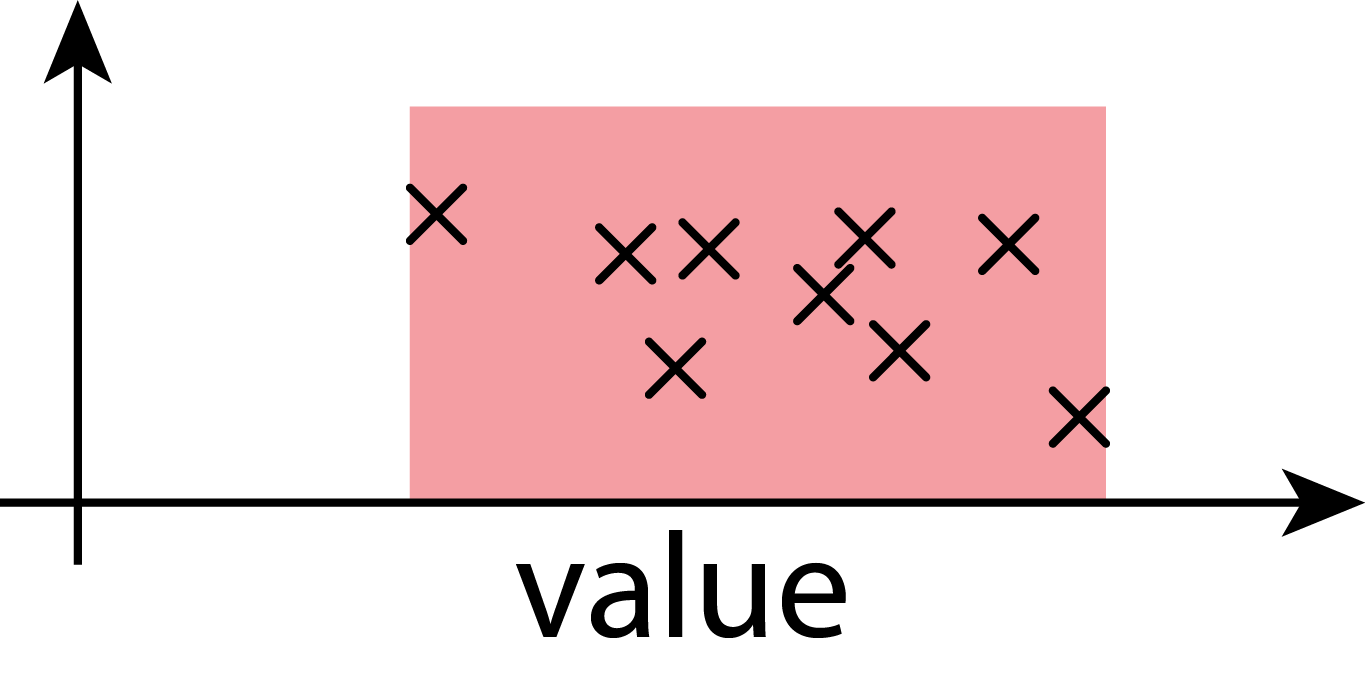
\includegraphics[width=0.95\linewidth,height=\textheight,keepaspectratio]{chapter000/spread_ds.png}

}

\caption{\label{fig-spread}Spread, Dispersion, Variance \ldots{} many
names for measuring variability of data}

\end{figure}%

Measures of spread (also called measures of dispersion or variability)
are essential in statistics to provide information about the
distribution of data --- specifically, how much the data values differ
from each other and from the central tendency.

\begin{itemize}
\item
  Contextualizing Central Tendency: The mean or median alone does not
  give a complete picture of the data. Two datasets can have the same
  mean but very different spreads.
\item
  Understanding Data Consistency: Measures of spread indicate how
  consistent or reliable the data are. A small spread suggests the
  values are closely clustered around the mean, while a large spread
  indicates greater variability and less predictability.
\item
  Identifying Outliers: Large measures of spread may indicate the
  presence of outliers --- values that are significantly different from
  others in the dataset. This can be important in quality control, risk
  assessment, and anomaly detection.
\item
  Comparing Distributions: Spread allows for meaningful comparison
  between different datasets.
\item
  Informing Statistical Models: Many statistical methods, such as
  regression, hypothesis testing, and confidence intervals, rely on
  measures of spread (like variance or standard deviation) to estimate
  error, assess significance, or make predictions.
\end{itemize}

\subsubsection{Range}\label{range}

\begin{figure}[ht]

\centering{

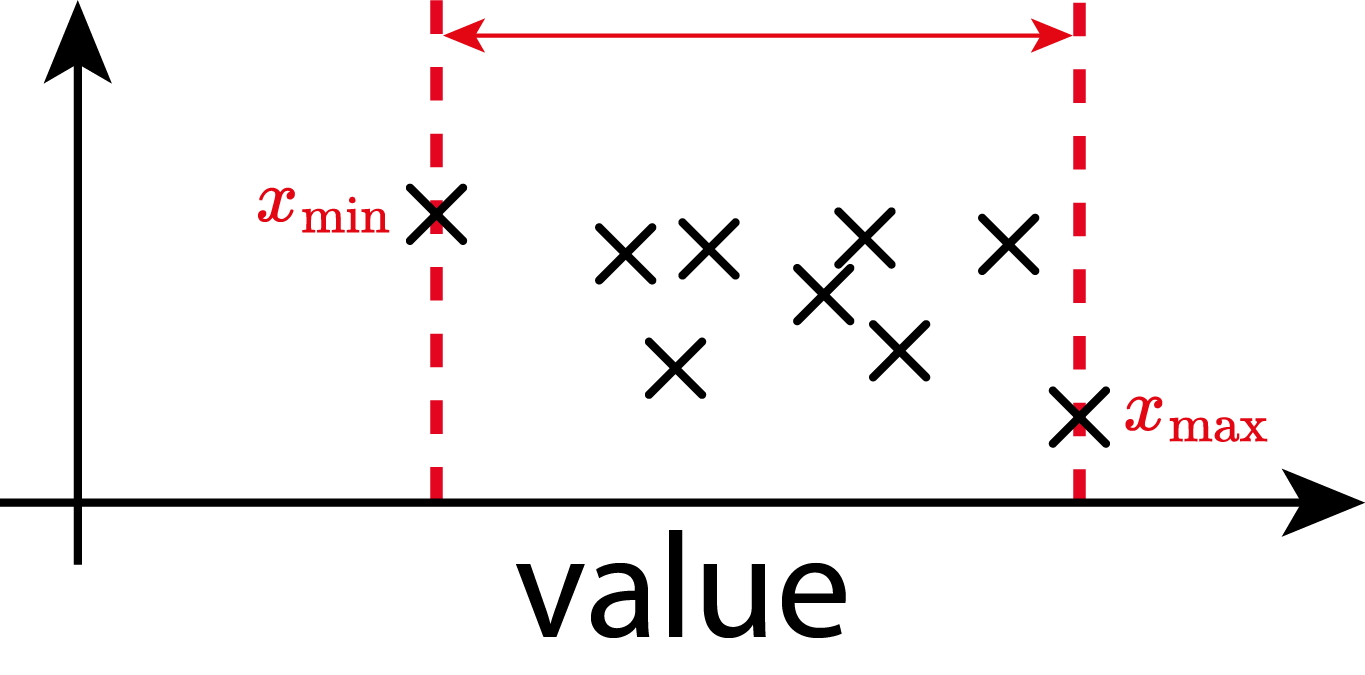
\includegraphics[width=0.95\linewidth,height=\textheight,keepaspectratio]{chapter000/range_ds.png}

}

\caption{\label{fig-range-ds}A graphical depiction of the range}

\end{figure}%

\begin{align}
\text{Range} = x_{\text{max}} - x_{\text{min}}
\end{align}

There is no difference in computing the range for the population or the
sample

\subsubsection{Variance}\label{variance}

\begin{figure}[ht]

\centering{

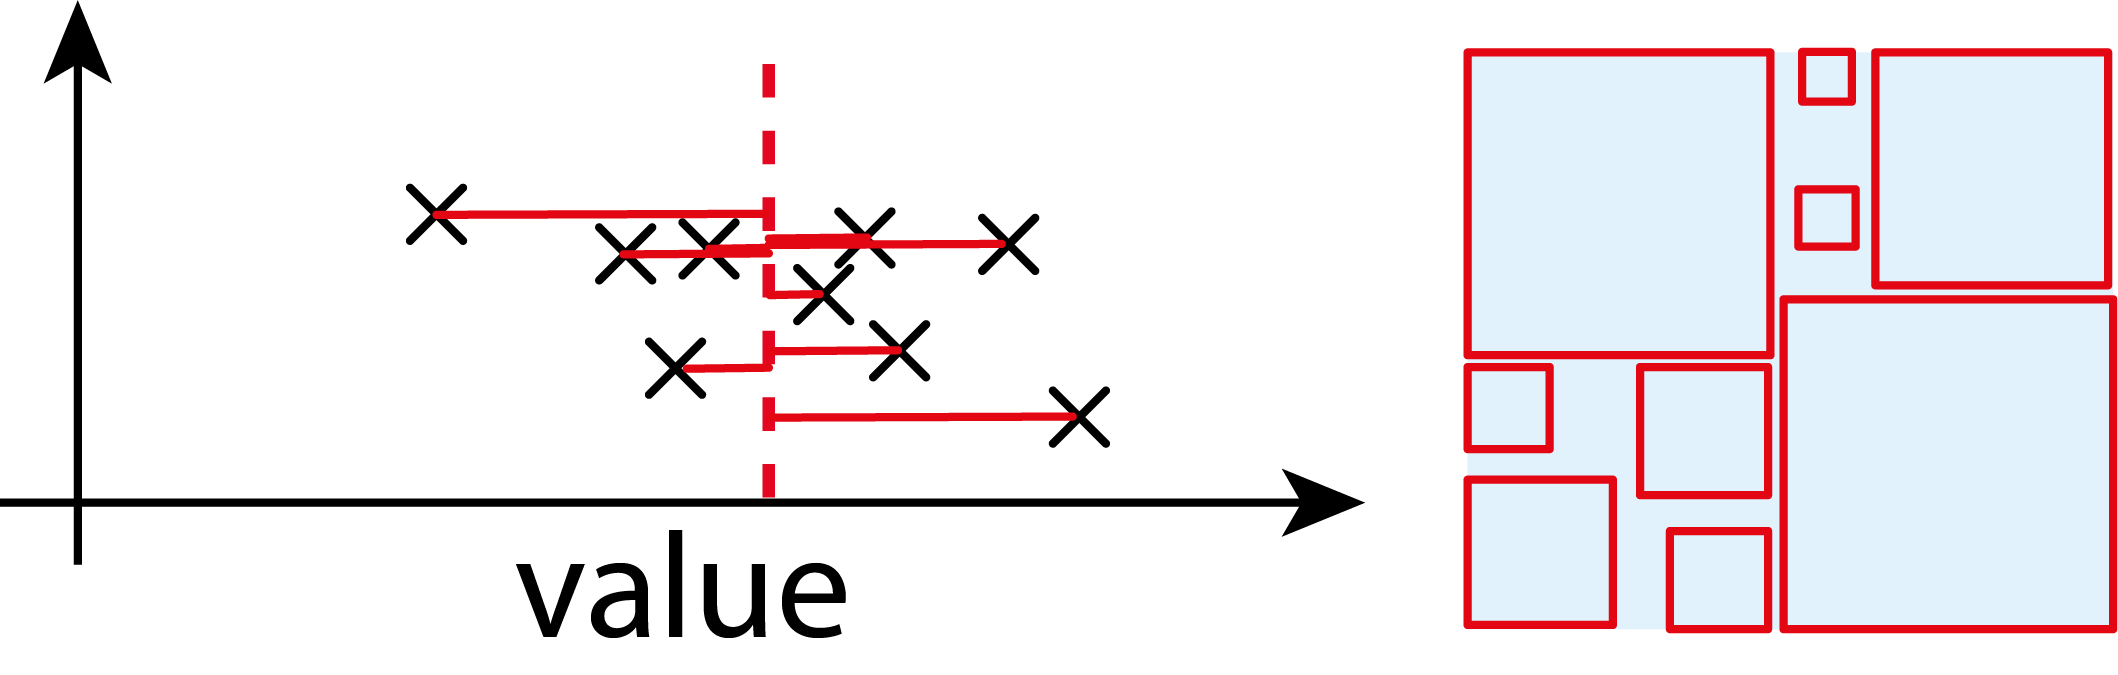
\includegraphics[width=0.75\linewidth,height=\textheight,keepaspectratio]{chapter000/variance_ds.png}

}

\caption{\label{fig-variance-ds}A graphical depiction of the variance}

\end{figure}%

For a random variable \(X\) with mean \(\mu=\mathbb{E}\!(X)\):

\begin{align}
\mathrm{Var}(X) &= \mathbb{E}\!\big[(X - \mu)^2\big] \label{var} \\
\mathrm{Var}(X) &= \mathbb{E}[X^2] - \big(\mathbb{E}[X]\big)^2
\end{align}

It is the \textbf{expected squared deviation} from the mean.

\begin{itemize}
\item
  Always non-negative.
\item
  Units: square of the units of \(X\)
\end{itemize}

\subsubsection{Standad Deviation}\label{standad-deviation}

\begin{align}
\sigma_0 &= \sqrt{\mathrm{Var}}
\end{align}

\begin{align}
\text{population: } \sigma &= \sqrt{\frac{1}{N} \sum_{i=1}^{N} (x_i - \mu)^2}\\
\text{sample: } sd &= \sqrt{\frac{1}{n-1} \sum_{i=1}^{n} (x_i - \bar{x})^2}
\end{align}

\begin{figure}[ht]

\centering{

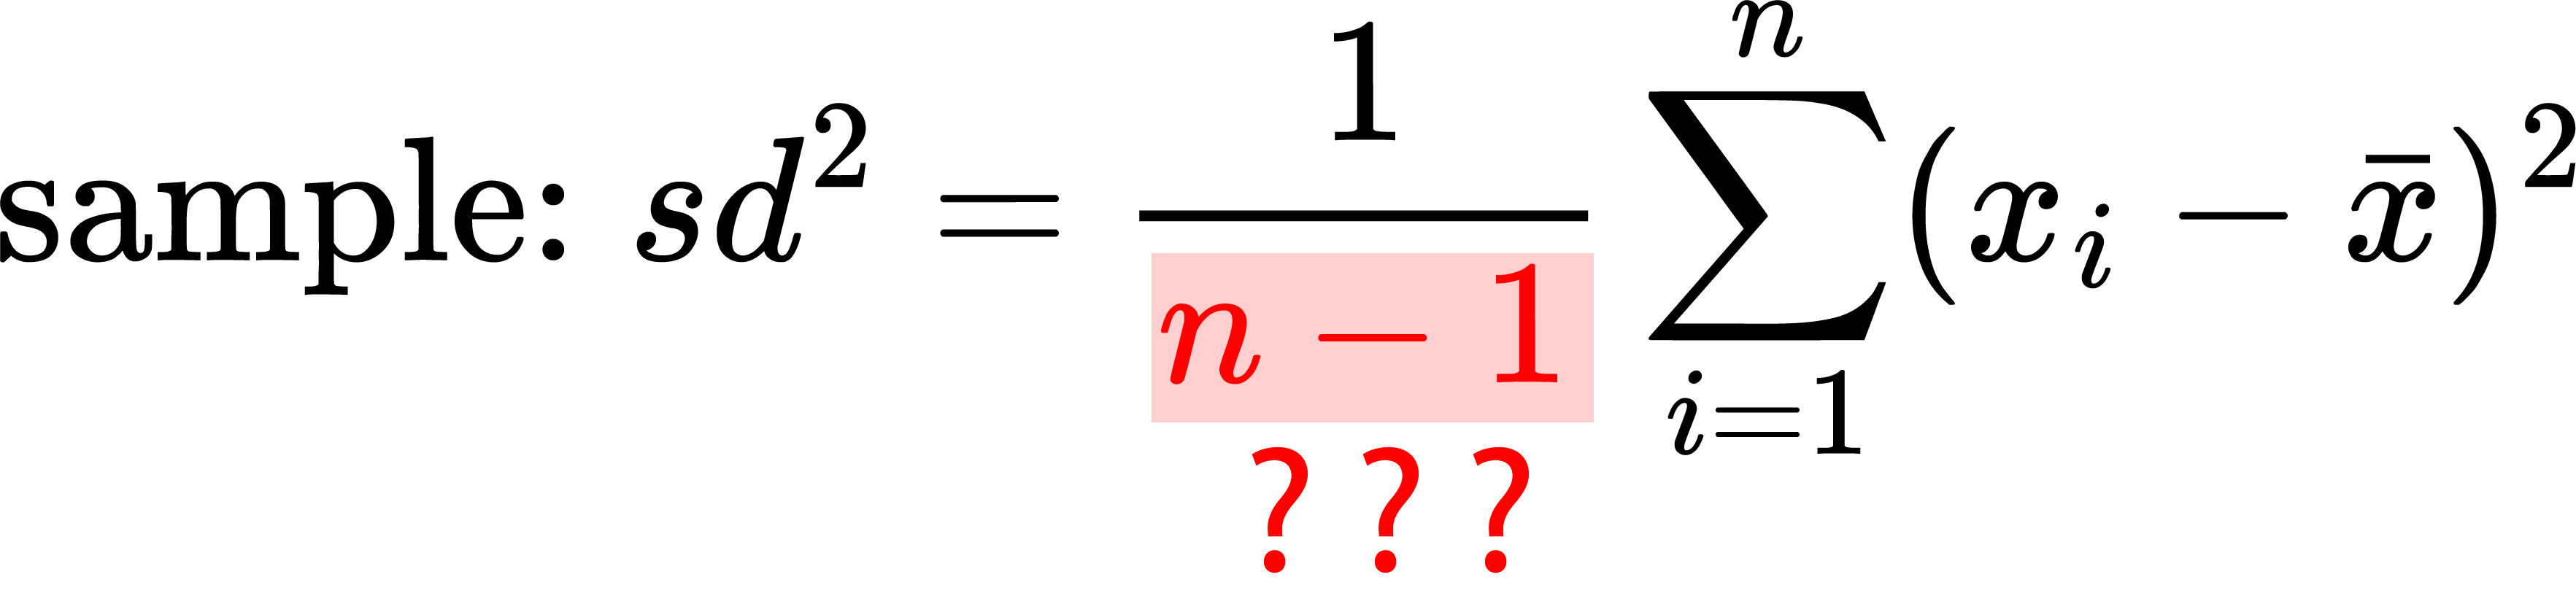
\includegraphics[width=0.95\linewidth,height=\textheight,keepaspectratio]{chapter000/bessel_intro.png}

}

\caption{\label{fig-bessel-intro}Why do we divide by n-1 for the sample
variance?}

\end{figure}%

\paragraph{The Bessel's correction}\label{the-bessels-correction}

The variance calculated from a sample has one
\hyperref[acronyms_dof]{degree of freedom (dof)} less, then the
population variance.

Imagine you have 5 candies, and you want to give them to 5 friends ---
one candy to each. You decide how to give the first candy, then the
second, third, and fourth. But when you get to the last candy, you have
no choice --- you have to give it to the last friend, so everyone gets
one.

That's kind of like degrees of freedom in statistics. It means how many
things you're free to choose before something has to be a certain way.

So if you're working with 5 numbers, and they all have to add up to a
certain total (like a mean), you can choose 4 of them freely, but the
last one has to be whatever makes the total come out right. That's why
we say there are 4 degrees of freedom --- 4 numbers you can choose any
way you want.

\[\{2,4,6\}\]

\begin{itemize}
\tightlist
\item
  Mean: \(\bar{x} = \frac{2+4+6}{3} = 4\)
\item
  Deviations: \(-2,0,2\)
\item
  Squared Deviations: \(4,0,4\)
\item
  Sum of squared deviations: \(8\)
\end{itemize}

\textbf{with Bessel's correction: } \(sd^2 = \frac{8}{3-1} = 4\)

\textbf{without Bessel's correction: }
\(sd^2 = \frac{8}{3} \approx 2.67\) (biased, underestimates variance)

When computing the variance from a sample, we need to calculate
\(\bar{x}\), which \emph{uses up} one degree of freedom and biases our
estimate

\paragraph{Bessel's correction with increasing sample
size}\label{bessels-correction-with-increasing-sample-size}

\begin{figure}[ht]

\centering{

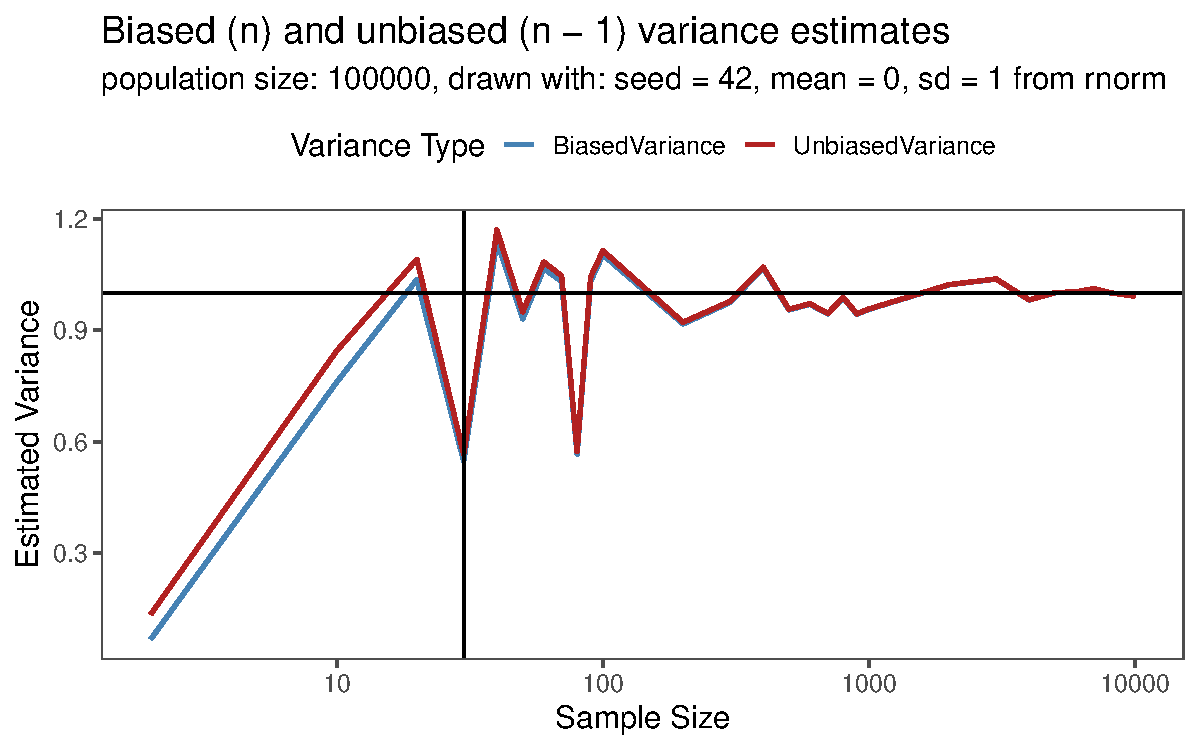
\includegraphics[width=0.95\linewidth,height=\textheight,keepaspectratio]{chapter000_BasicConcepts_files/figure-pdf/fig-bessel-large-n-1.pdf}

}

\caption{\label{fig-bessel-large-n}The biased (n) variance is not as
prcises as the unbiased (n-1) variance estimate. This effect decreases
with increasing sample size.}

\end{figure}%

\subsubsection{Percentiles, quantiles}\label{percentiles-quantiles}

\begin{itemize}
\item
  Percentiles: Divide data into \(100\) equal parts. The \(p\)th
  percentile is the value below which p\% of the observations fall.
\item
  Quantiles: Generalization of percentiles. The q-th quantile is the
  value below which a fraction q of the data falls. For example:

  \begin{itemize}
  \item
    \(0.25\) quantile: \(25\)th percentile - first quartile (Q1)
  \item
    \(0.50\) quantile: \(50\)th percentile - median
  \item
    \(0.75\) quantile: \(75\)th percentile - third quartile (Q3)
  \end{itemize}
\end{itemize}

\begin{figure}[ht]

\centering{

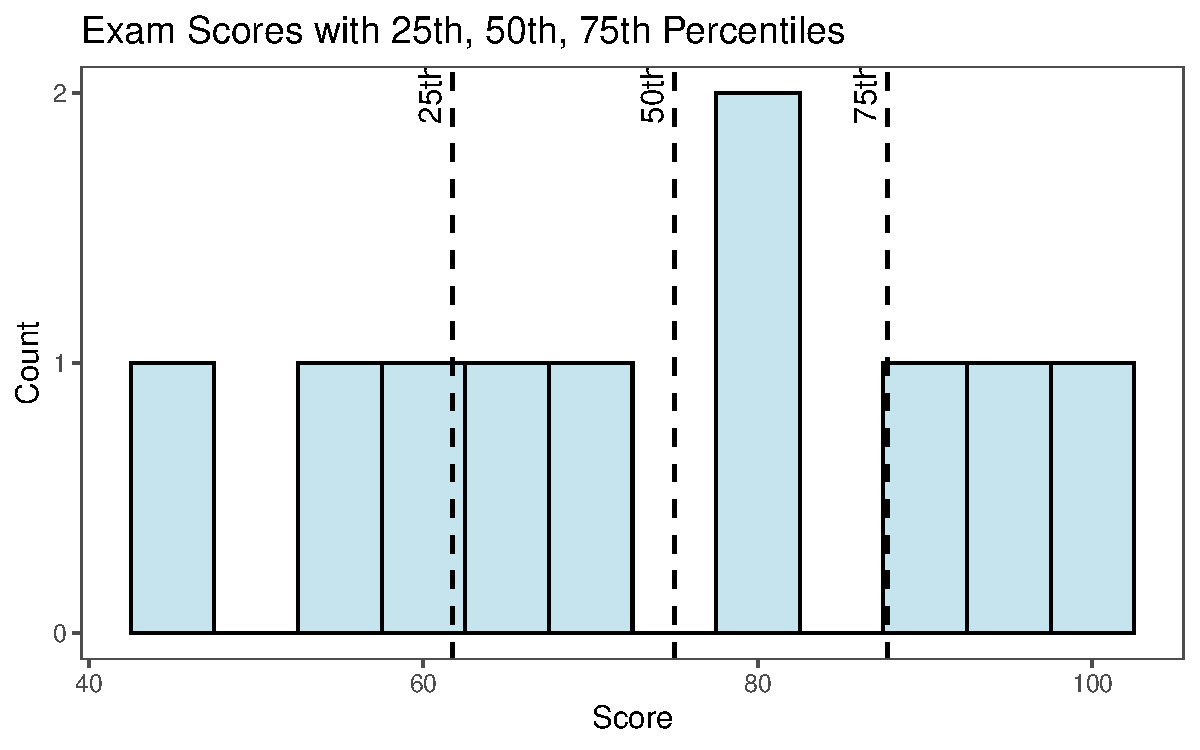
\includegraphics[width=0.95\linewidth,height=\textheight,keepaspectratio]{chapter000_BasicConcepts_files/figure-pdf/fig-percentile-quantile-1.pdf}

}

\caption{\label{fig-percentile-quantile}A graphical depiction of various
percentiles, quantiles}

\end{figure}%

\subsection{Histogram}\label{histogram}

\begin{figure}[ht]

\centering{

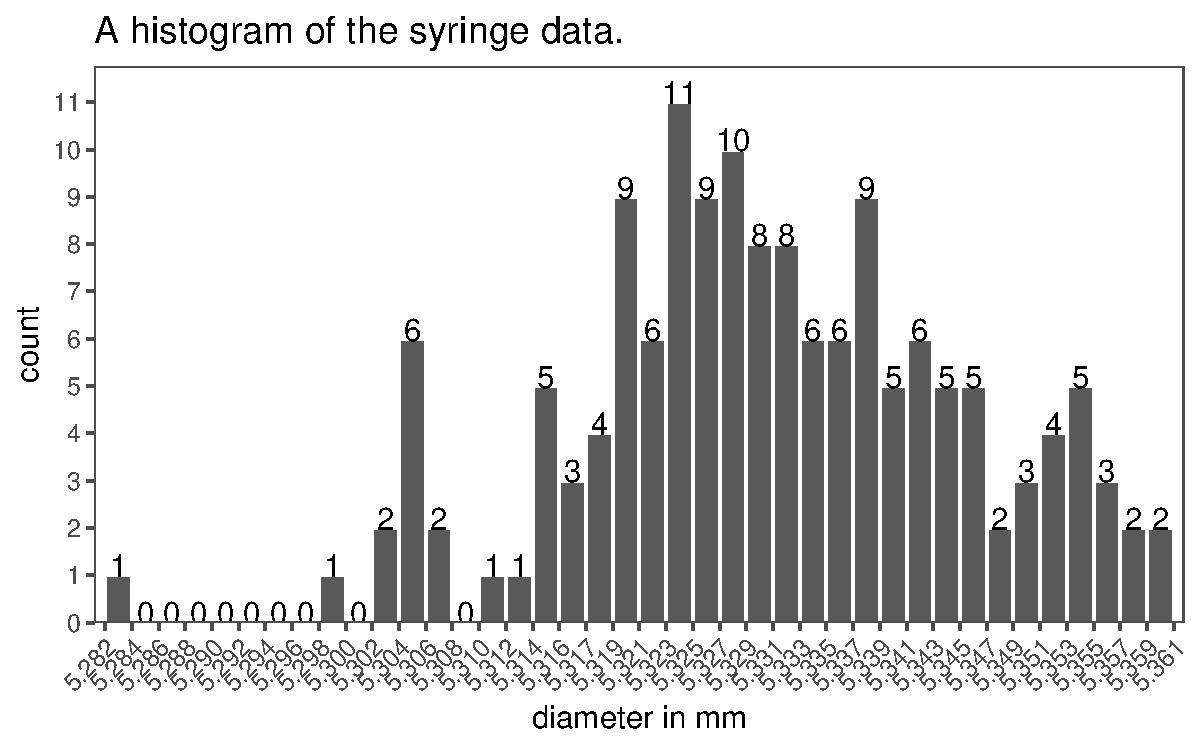
\includegraphics[width=0.95\linewidth,height=\textheight,keepaspectratio]{chapter000_BasicConcepts_files/figure-pdf/fig-plot-sample-001-1.pdf}

}

\caption{\label{fig-plot-sample-001}An example for descriptive
statistics (histogramm)}

\end{figure}%

An example for descriptive statistics is shown in
Figure~\ref{fig-plot-sample-001} as a histogram. It shows data from a
company that produces pharmaceutical syringes, taken from Ramalho
(2021). During the production of those syringes, the so called
\emph{barrel diameter} is a critical parameter to the function of the
syringe and therefore of special interest for the \hyperref[QC]{Quality
Control}.

A histogram as shown in Figure~\ref{fig-plot-sample-001} shows the data
of 150 measurements during the \hyperref[QC]{QC}. On the \texttt{x-axis}
the \emph{barrel diameter} is shown, while the count of each
\emph{binned} diameter is shown on the \texttt{y-axis}. The binning and
of data is a crucial parameter for such a plot, because it already
changes the appearance and width of the bars. Binning is a trade-off
between visibility and readability.

\subsection{Density plot}\label{density-plot}

\begin{figure}[ht]

\centering{

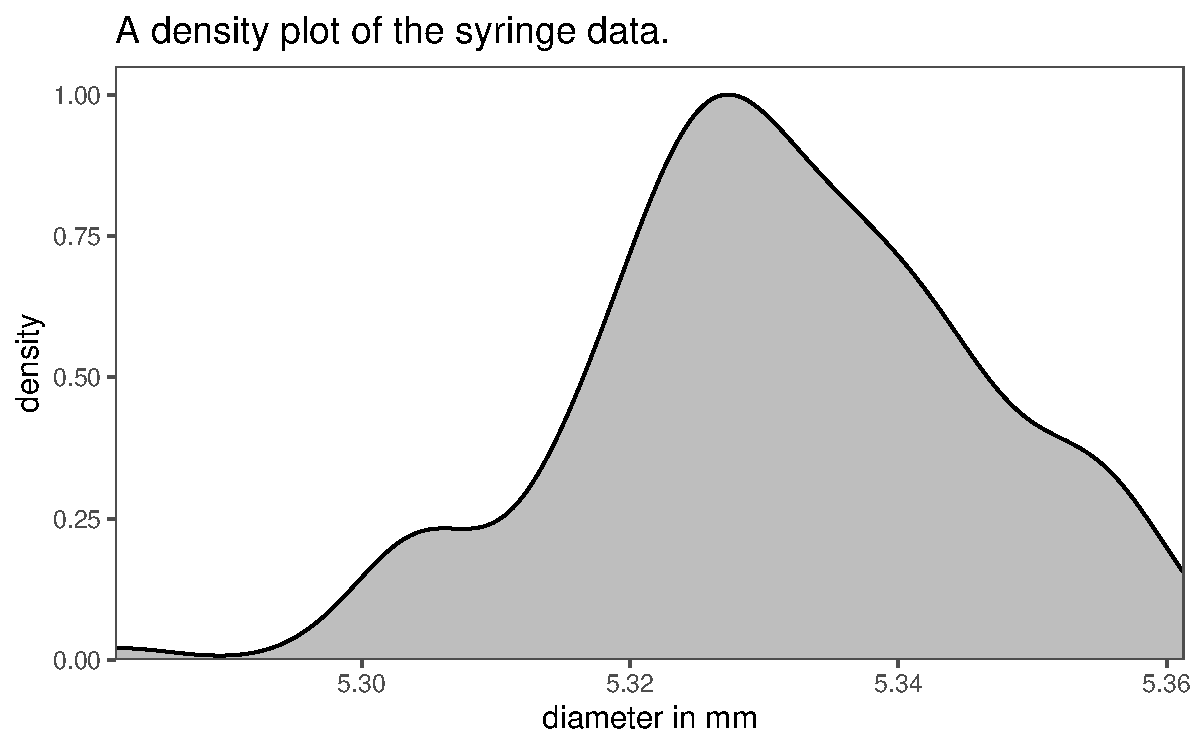
\includegraphics[width=0.95\linewidth,height=\textheight,keepaspectratio]{chapter000_BasicConcepts_files/figure-pdf/fig-plot-density-1.pdf}

}

\caption{\label{fig-plot-density}An example for a density plot for the
syringe data (barrel diameter).}

\end{figure}%

Density plots are another way of displaying the statistical distribution
of an underlying dataset. The biggest strength of those plots is, that
no binning is necessary in order to show the data. The limitation of
this kind of plot is the interpretability. An example of a density plot
for the syringe data is shown in Figure~\ref{fig-plot-density}. On the
\texttt{x-axis} the syringe barrel diameter is shown (as in a
histogram). The \texttt{y-axis} in contrast does not display the count
of a binned category, but rather the \hyperref[acronyms_PDF]{Probability
Density Function (PDF)} for the specific diameter. The grey area under
the density curve depicts the probability of a syringe diameter to
appear in the data. The complete area under the curve equals to \(1\)
meaning that a certain diameter is sure to appear in the data.

\subsection{Boxplot}\label{boxplot}

\begin{figure}[H]

\centering{

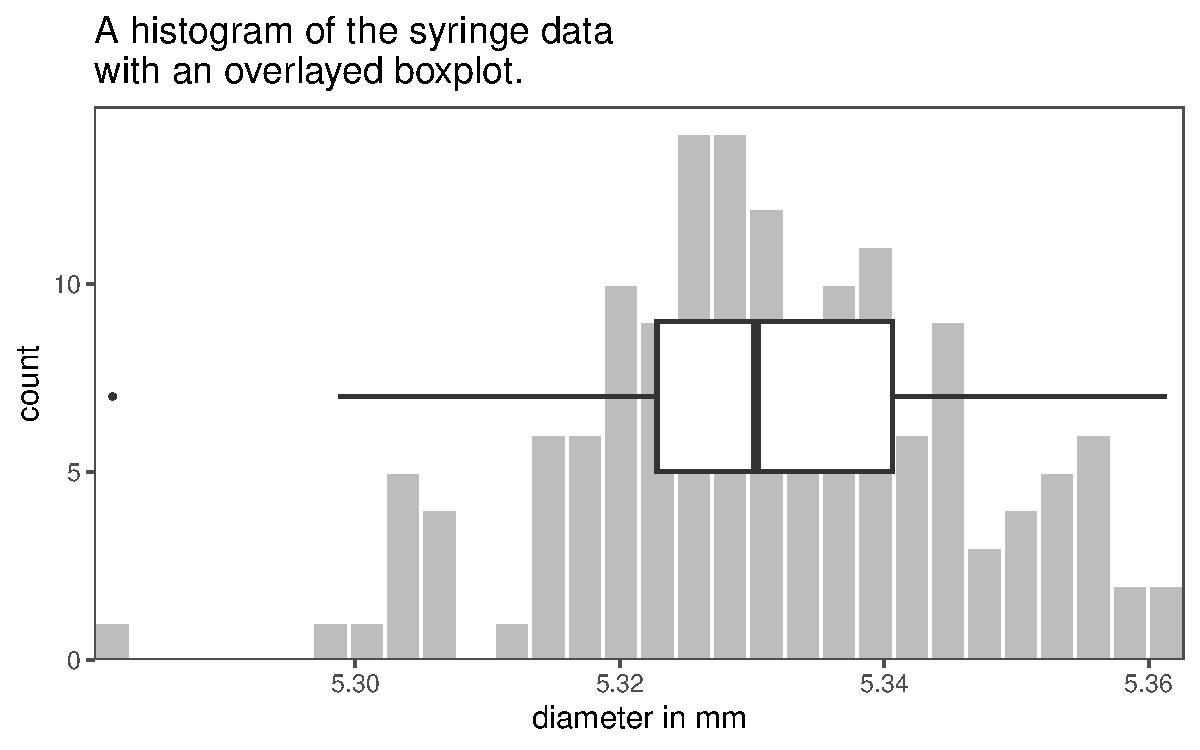
\includegraphics[width=0.95\linewidth,height=\textheight,keepaspectratio]{chapter000_BasicConcepts_files/figure-pdf/fig-plot-sample-003-1.pdf}

}

\caption{\label{fig-plot-sample-003}A boxplot of the same syringe data
combined with the according histogram.}

\end{figure}%

It is very common to include and inspect measures of central tendency in
the graphical depiction of data. A \texttt{boxplot}, also known as a
box-and-whisker plot, is a very common way of doing this. A
\texttt{boxplot} is a graphical representation of a dataset's
distribution. It displays the following key statistics:

\begin{enumerate}
\def\labelenumi{\arabic{enumi}.}
\tightlist
\item
  Median (middle value).
\item
  Quartiles (\(25^{th}\) and \(75^{th}\) percentiles), forming a box.
\item
  Minimum and maximum values (whiskers).
\item
  Outliers (data points significantly different from the rest).
\end{enumerate}

The syringe data in boxplot form is shown in
Figure~\ref{fig-plot-sample-003} as an overlay of the histogram plot
before. Boxplots are useful for quickly understanding the central
tendency, spread, and presence of outliers in a dataset, making them a
valuable tool in data analysis and visualization.

\subsection{Average, Standard deviation and
Range}\label{average-standard-deviation-and-range}

\begin{figure}[ht]

\centering{

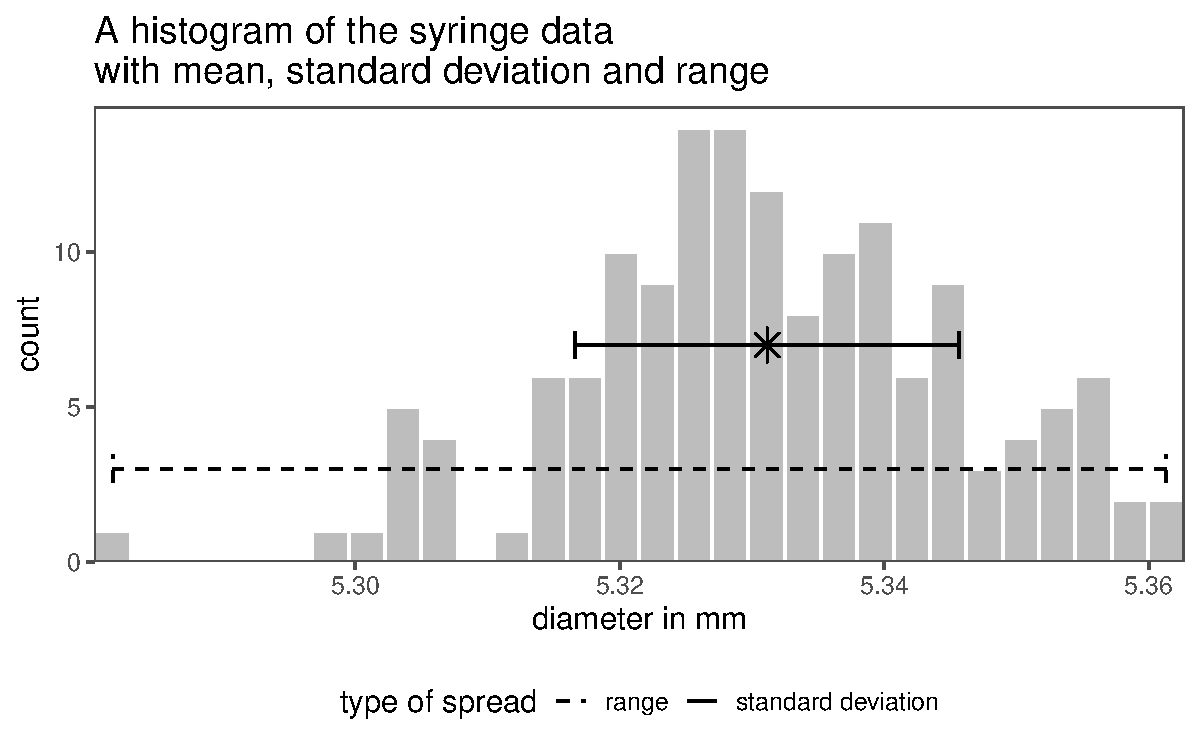
\includegraphics[width=0.95\linewidth,height=\textheight,keepaspectratio]{chapter000_BasicConcepts_files/figure-pdf/fig-plot-sample-031-1.pdf}

}

\caption{\label{fig-plot-sample-031}A histogram of the syringe data with
mean, standard deviation and range.}

\end{figure}%

Very popular measures of central tendency include the \emph{average}
(mean) and the \emph{standard deviation} (variance) of a dataset. The
computed mean from an actual dataset is depicted with
\hyperref[mean-gloss]{\(\bar{x}\)} and calculated via \eqref{mean}.

\begin{align}
\bar{x} = \frac{1}{n}\sum_{i=1}^{n} x_i \label{mean}
\end{align}

With {[}\(n\){]}\{index.qmd\#n-gloss\} being the number of datapoints
and \hyperref[xi-gloss]{\(x_i\)} being the datapoints. The \emph{mean}
is therefore the sum of all datapoints divided by the total number \(n\)
of all datapoints. It is not to be confused with the true mean
\hyperref[truemean-gloss]{\(\mu_0\)} of a population.

The computed \emph{standard deviation} from an actual dataset is
depicted with {[}\(sd\){]}\{index.qmd\#sd-gloss\} and calculated via
\eqref{sd}.

\begin{align}
sd = \sqrt{\frac{1}{n} \sum_{i=1}^{n} (x_i - \bar{x})^2} \label{sd}
\end{align}

The \emph{standard deviation} can therefore be explained as the square
root of the sum of all differences of each individual datapoints to the
mean of a dataset divided by the number of datapoints. It is not to be
confused with the true variance
\hyperref[truevariance-gloss]{\(\sigma_0^2\)} of a population. The
variance of a dataset can be calculated via \eqref{var2}.

\begin{align}
\sigma = sd^2 \label{var2}
\end{align}

The \emph{range} from an actual dataset is depicted with
\hyperref[range-gloss]{\(r\)} and calculated via \eqref{range}.

\begin{align}
r = \max(x_i) - \min(x_i) \label{range}
\end{align}

The \emph{range} can therefore be interpreted as the range from minimum
to maximum in a dataset.

\section{Visualizing Groups}\label{sec-vis-grps}

\subsection{Boxplots}\label{boxplots}

\begin{figure}[ht]

\centering{

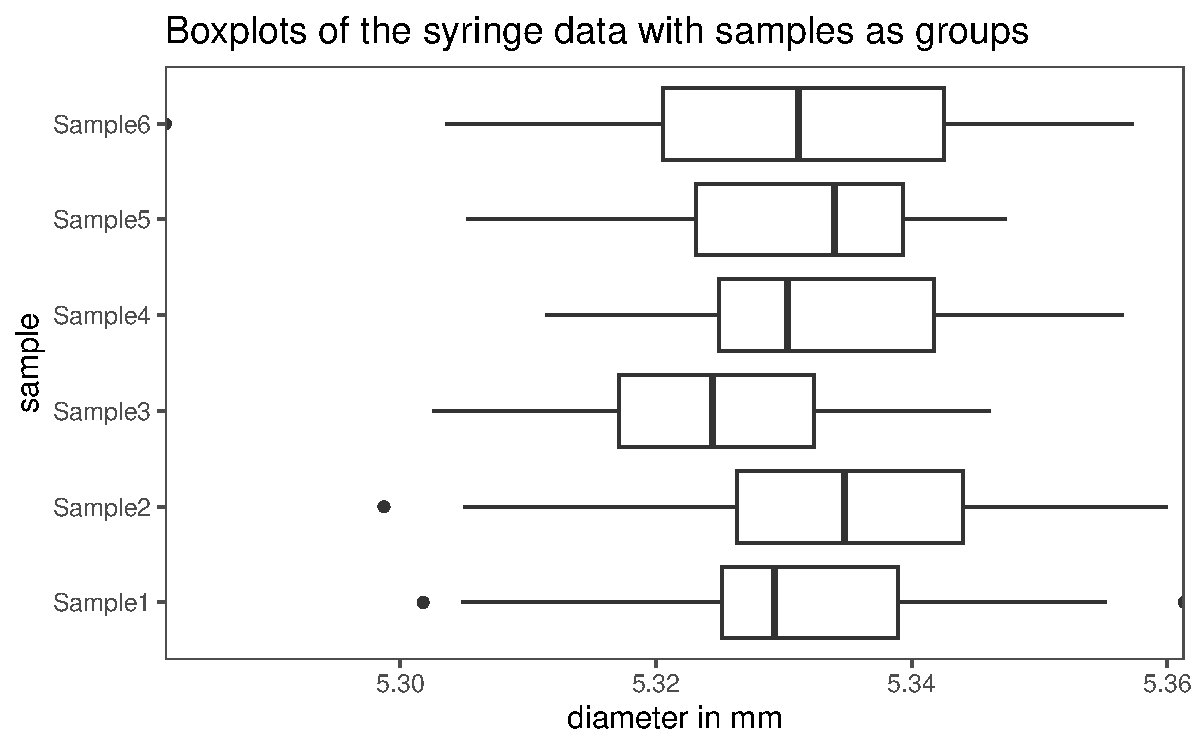
\includegraphics[width=0.95\linewidth,height=\textheight,keepaspectratio]{chapter000_BasicConcepts_files/figure-pdf/fig-groups-boxplot-1.pdf}

}

\caption{\label{fig-groups-boxplot}Boxplots of the syringe data with the
samples as groups.}

\end{figure}%

The methods described above are especially useful when it comes to
visualizing groups in data. The data is discretized and the information
density is increased. As with every discretization comes also a loss of
information. It is therefore strongly advised to choose the right tool
for the job.

If the underlying distribution of the data is unknown, a good start to
visualize groups within data is usually a boxplot as shown in
Figure~\ref{fig-groups-boxplot}. The syringe data from Ramalho (2021)
contains six different groups, one for every sample drawn. Each sample
consists of 25 observations in total. On the \texttt{x-axis} the
\emph{diameter} in mm is shown, the \texttt{y-axis} depicts the sample
number. The \texttt{boxplots} are then drawn as described above (median,
\(25^{th}\) and \(75^{th}\) percentile box, \(5^{th}\) and \(95^{th}\)
whisker). The \(25^{th}\) and \(75^{th}\) percentile box is also known
as the \hyperref[acronyms_IQR]{Interquartile Range (IQR)}.

\subsection{Mean and standard deviation
plots}\label{mean-and-standard-deviation-plots}

\begin{figure}[ht]

\centering{

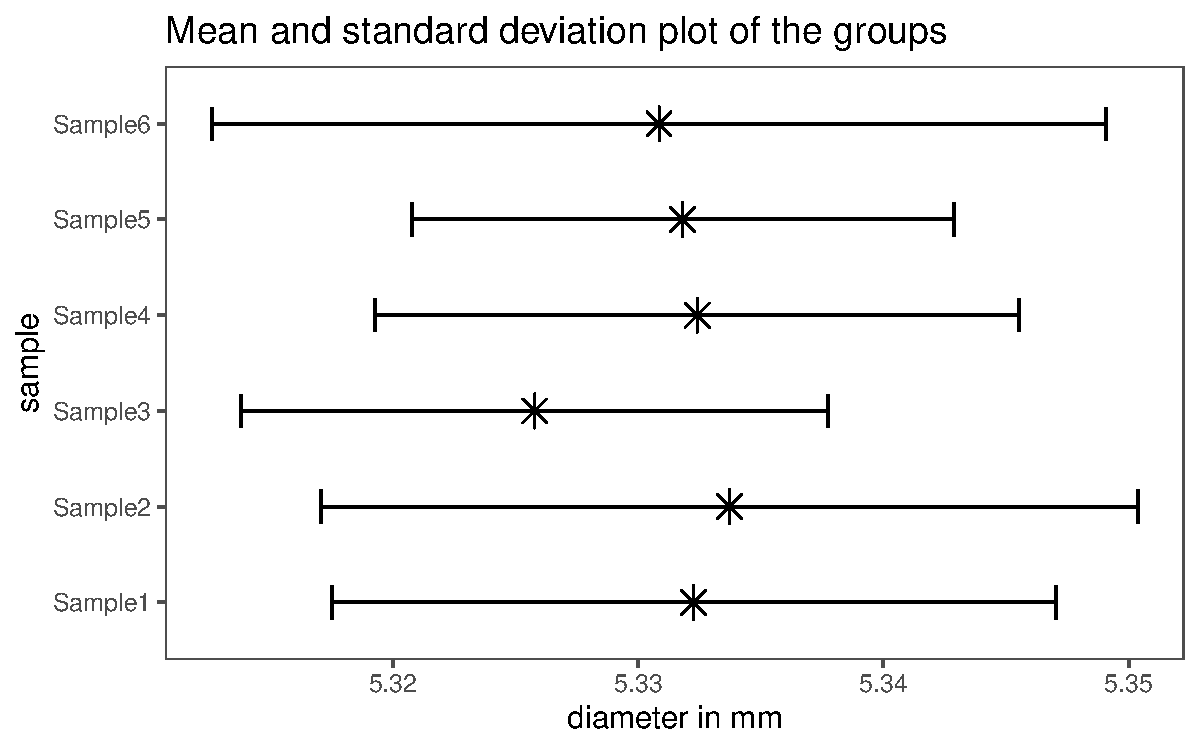
\includegraphics[width=0.95\linewidth,height=\textheight,keepaspectratio]{chapter000_BasicConcepts_files/figure-pdf/fig-groups-mean-sd-1.pdf}

}

\caption{\label{fig-groups-mean-sd}Mean and standard deviation plots of
the groups in the dataset.}

\end{figure}%

If the data follows a normal distribution, showing the mean and standard
deviation for each group is also very common. For the syringe dataset,
this is shown in Figure~\ref{fig-groups-mean-sd}. The plot follows the
same logic as for the boxplots (\texttt{x-axis-data},
\texttt{y-axis-data}), but the data itself shows the mean with a
\(\times\)-symbol, as the length of the horizontal errorbars accords to
\(\bar{x} \pm sd(x)\).

\subsection{Half-half plots}\label{half-half-plots}

\begin{figure}[ht]

\centering{

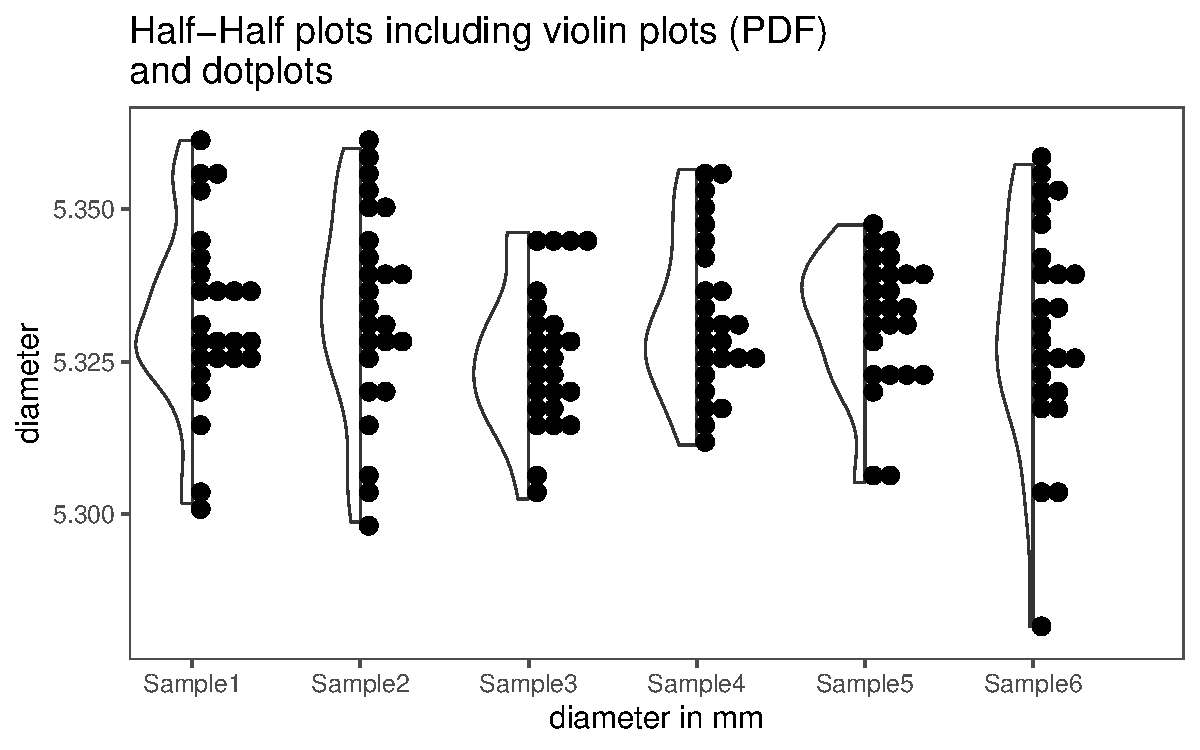
\includegraphics[width=0.95\linewidth,height=\textheight,keepaspectratio]{chapter000_BasicConcepts_files/figure-pdf/fig-groups-halves-1.pdf}

}

\caption{\label{fig-groups-halves}Half-half plots that incooperate
different types of plots}

\end{figure}%

Boxplots and mean-and-standard-deviation plots sometimes hide some
details within the data, that may be of interest or simply important.
Half-half plots, as shown in shown in Figure~\ref{fig-groups-halves},
incorporate different plot mechanisms. The left half shows a violin
plot, which outlines the underlying distribution of the data using the
\hyperref[acronyms_PDF]{PDF}. This is very similar to a density plot.
The right half shows the original data points and give the user a
visible clue about the sample size in the data size. Note that the
\texttt{y}-position of the points is jittered to counter
\emph{overplotting}. Details can be found in Tiedemann (2022).

\subsection{Ridgeline plots}\label{ridgeline-plots}

\begin{figure}[ht]

\centering{

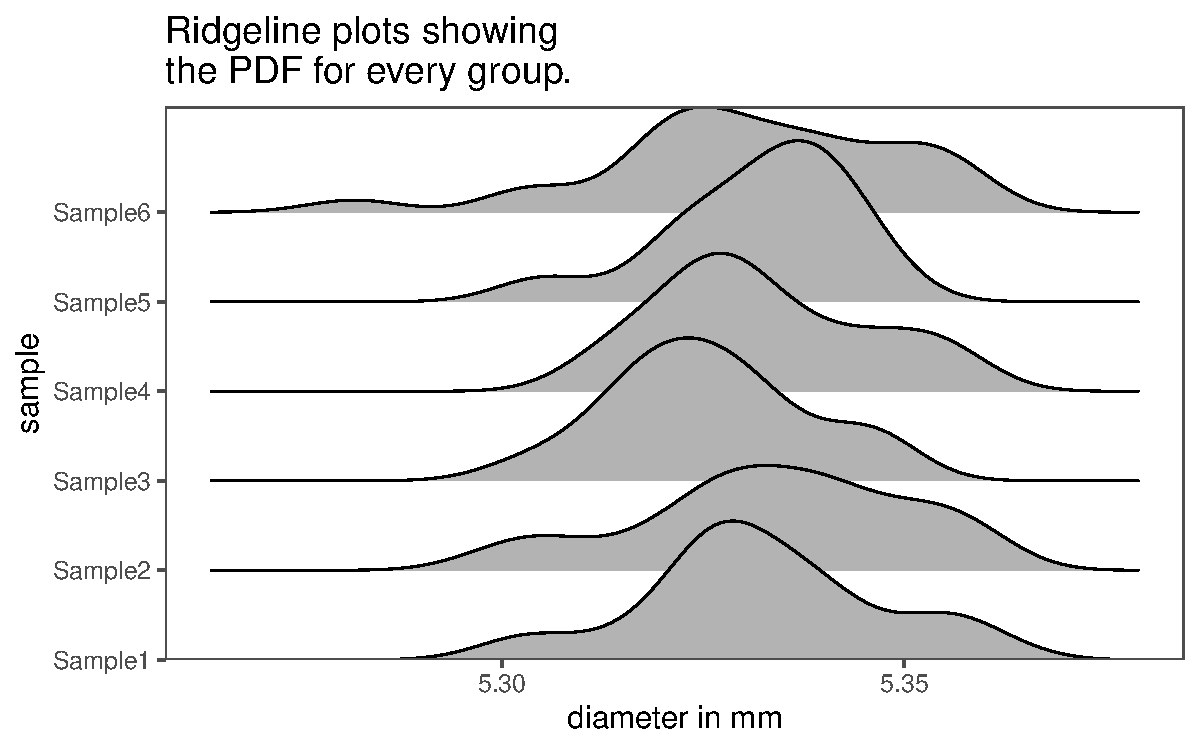
\includegraphics[width=0.95\linewidth,height=\textheight,keepaspectratio]{chapter000_BasicConcepts_files/figure-pdf/fig-groups-ridge-1.pdf}

}

\caption{\label{fig-groups-ridge}Ridgeline plots for distributions
within groups.}

\end{figure}%

Figure~\ref{fig-groups-ridge} shows so called \emph{ridgeline} plots as
explained in Wilke (2022). They are in essence density plots that use
the \texttt{y-axis} to differentiate between the groups. On the
\texttt{x-axis} the density of the underlying dataset is shown. More
info on the creation of these plots and graphics is available in Wickham
(2016) as well as {``The {R} Graph Gallery -- Help and Inspiration for r
Charts''} (2022).

\section{The drive shaft exercise}\label{the-drive-shaft-exercise}

\subsection{Introduction}\label{introduction}

\begin{figure}[ht]

\centering{

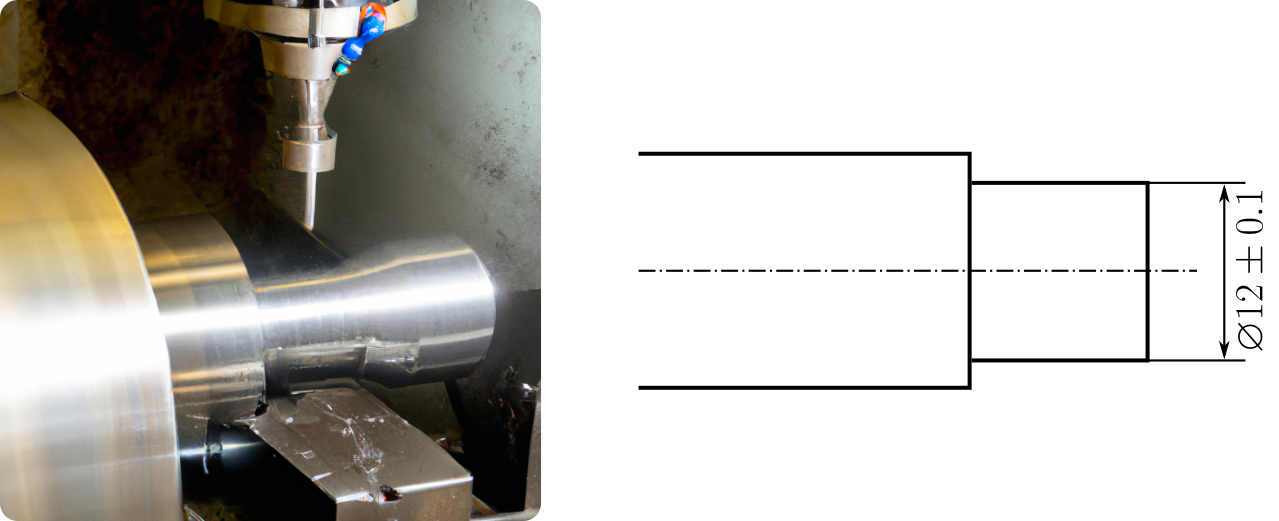
\includegraphics[width=0.95\linewidth,height=\textheight,keepaspectratio]{chapter000/005_DriveShaft.png}

}

\caption{\label{fig-drive-shaft-spec}The drive shaft specification.}

\end{figure}%

A drive shaft is a mechanical component used in various vehicles and
machinery to transmit rotational power or torque from an engine or motor
to the wheels or other driven components. It serves as a linkage between
the power source and the driven part, allowing the transfer of energy to
propel the vehicle or operate the machinery.

\begin{enumerate}
\def\labelenumi{\arabic{enumi}.}
\item
  Material Selection: Quality steel or aluminum alloys are chosen based
  on the specific application and requirements.
\item
  Cutting and Machining: The selected material is cut and machined to
  achieve the desired shape and size. Precision machining is crucial for
  balance and performance.
\item
  Welding or Assembly: Multiple sections may be welded or assembled to
  achieve the required length. Proper welding techniques are used to
  maintain structural integrity.
\item
  Balancing: Balancing is critical to minimize vibrations and ensure
  smooth operation. Counterweights are added or mass distribution is
  adjusted.
\item
  Surface Treatment: Drive shafts are often coated or treated for
  corrosion resistance and durability. Common treatments include
  painting, plating, or applying protective coatings.
\item
  Quality Control: Rigorous quality control measures are employed to
  meet specific standards and tolerances. This includes dimensional
  checks, material testing, and defect inspections.
\item
  Packaging and Distribution: Once quality control is passed, drive
  shafts are packaged and prepared for distribution to manufacturers of
  vehicles or machinery.
\end{enumerate}

The end diameter of a drive shaft is primarily determined by its torque
capacity, length, and material selection. It needs to be designed to
handle the maximum torque while maintaining structural integrity and
flexibility as required by the specific application. For efficient load
transfer, there are ball bearings mounted on the end diameter. Ball
bearings at the end diameter of a drive shaft support its rotation,
reducing friction. They handle axial and radial loads, need lubrication
for longevity, and may include seals for protection. Proper alignment
and maintenance are crucial for their performance and customization is
possible to match specific requirements.

The end diameter of the drive shaft shall be \(\varnothing 12\pm0.1mm\)
(see Figure~\ref{fig-drive-shaft-spec}). This example will haunt us the
rest of this lecture.

\subsection{Visualizing all the Data}\label{visualizing-all-the-data}

\begin{figure}[ht]

\begin{minipage}{0.50\linewidth}

\centering{

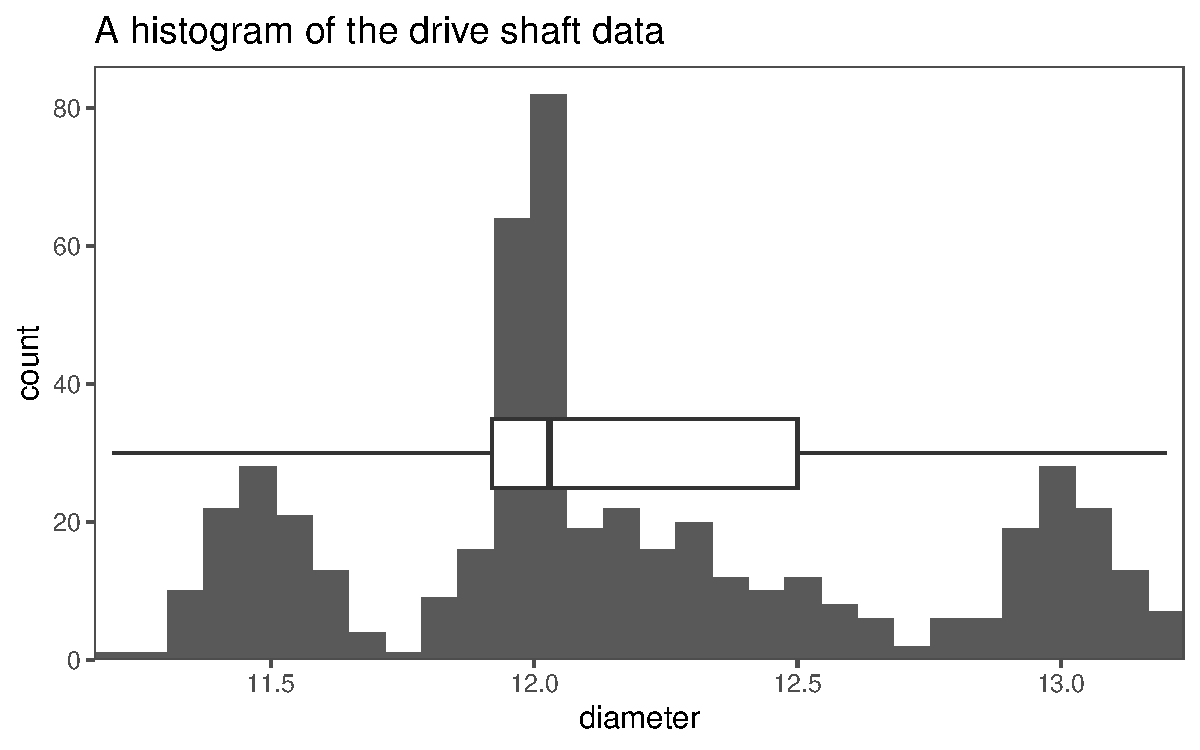
\includegraphics[width=0.95\linewidth,height=\textheight,keepaspectratio]{chapter000_BasicConcepts_files/figure-pdf/fig-ds-dist-1.pdf}

}

\subcaption{\label{fig-ds-dist-1}The drive shaft data shown in a
histogram.}

\end{minipage}%
%
\begin{minipage}{0.50\linewidth}

\centering{

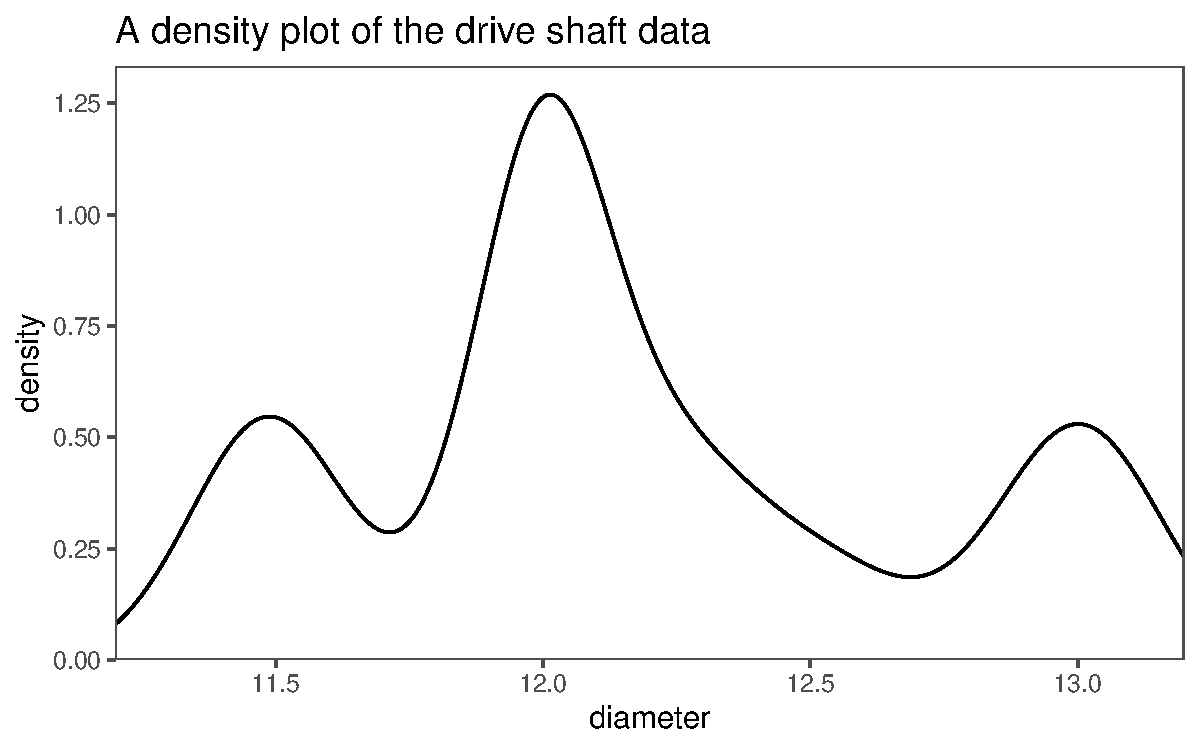
\includegraphics[width=0.95\linewidth,height=\textheight,keepaspectratio]{chapter000_BasicConcepts_files/figure-pdf/fig-ds-dist-2.pdf}

}

\subcaption{\label{fig-ds-dist-2}The drive shaft data shown in a density
plot.}

\end{minipage}%

\caption{\label{fig-ds-dist}The raw data of the measured drive shaft
diameter.}

\end{figure}%

First, some descriptive statistics of \(N=500\) produced drive shafts
are shown in Table~\ref{tbl-ds-sum} (\(\bar{x}(sd), median(IQR)\)). This
first table does not tell us an awful lot about the sample, apart from
the classic statistical measures of central tendency and spread.

\begin{table}

\caption{\label{tbl-ds-sum}The summary table of the drive shaft data}

\centering{

\fontsize{12.0pt}{14.0pt}\selectfont
\begin{tabular*}{\linewidth}{@{\extracolsep{\fill}}lc}
\toprule
\textbf{Variable} & \textbf{N = 500}\textsuperscript{\textit{1}} \\ 
\midrule\addlinespace[2.5pt]
diameter & 12.17 (0.51), 12.03 (0.58) \\ 
\bottomrule
\end{tabular*}
\begin{minipage}{\linewidth}
\textsuperscript{\textit{1}}Mean (SD), Median (IQR)\\
\end{minipage}

}

\end{table}%

In Figure~\ref{fig-ds-dist} the data and the distribution thereof is
visualized using different modalities. The complete
\texttt{drive\ shaft\ data} is shown as a histogram
(Figure~\ref{fig-ds-dist-1}) and as a density plot
(Figure~\ref{fig-ds-dist-2}). A single boxplot is plotted over the
histogram data in Figure~\ref{fig-ds-dist-1}, providing a link to
Table~\ref{tbl-ds-sum} (median and \hyperref[acronyms_IQR]{IQR}). One
important conclusion may be draw from those plots already: There may be
more than one dataset hidden inside the data. We will explore this
possibility further.

\subsection{Visualizing groups within the
data}\label{visualizing-groups-within-the-data}

\begin{figure}[ht]

\begin{minipage}{0.50\linewidth}

\centering{

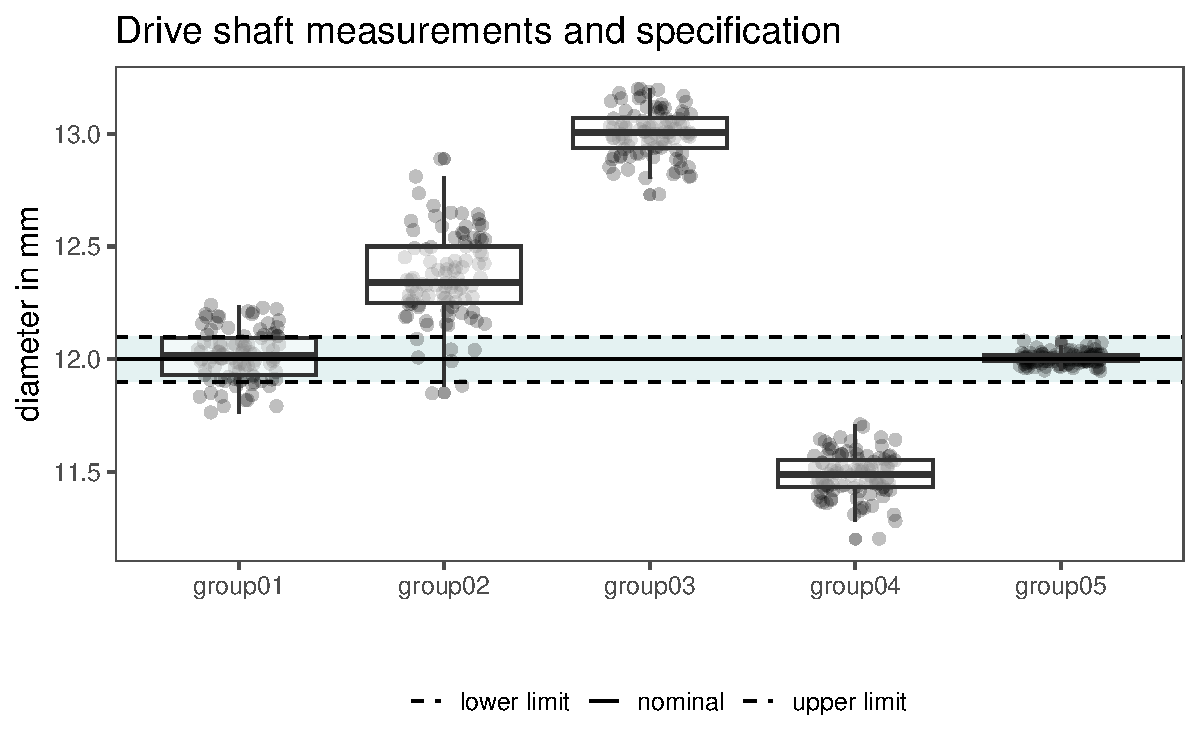
\includegraphics[width=0.95\linewidth,height=\textheight,keepaspectratio]{chapter000_BasicConcepts_files/figure-pdf/fig-ds-grps-1.pdf}

}

\subcaption{\label{fig-ds-grps-1}The groups visualized as boxplots
(including the specification)}

\end{minipage}%
%
\begin{minipage}{0.50\linewidth}

\centering{

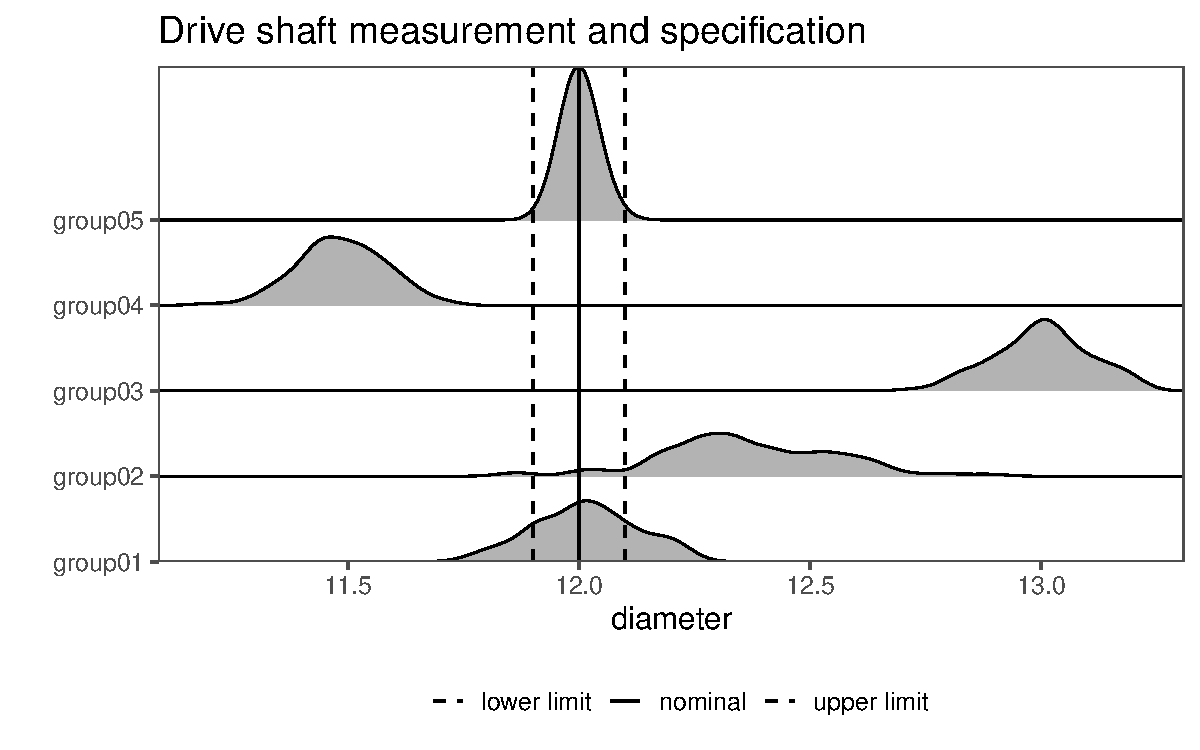
\includegraphics[width=0.95\linewidth,height=\textheight,keepaspectratio]{chapter000_BasicConcepts_files/figure-pdf/fig-ds-grps-2.pdf}

}

\subcaption{\label{fig-ds-grps-2}The groups visualized as ridgeline
plots}

\end{minipage}%

\caption{\label{fig-ds-grps}The raw data of the measured drive shaft
diameter.}

\end{figure}%

Fortunately for us, the groups that may be hidden within the data are
marked in the orginal dataset and denoted as \texttt{group0x}.
Unfortunately for us, it is not known (purely from the data) how these
groups come about. Because we did get the dataset from a colleague, we
need to investigate the \emph{creation} of the dataset even further.
This is an important point, for without knowledge about the history of
the data, it is \emph{impossible} or at least \emph{unadvisable} to make
valid statements about the data. We will go on with a table of summary
statistics, see Table~\ref{tbl-ds-sum-grps}. Surprisingly, there are
five groups hidden within the data, something we would no be able to
spot from the raw data alone.

\begin{table}

\caption{\label{tbl-ds-sum-grps}The group summary table of the drive
shaft data}

\centering{

\fontsize{12.0pt}{14.0pt}\selectfont
\begin{tabular*}{\linewidth}{@{\extracolsep{\fill}}lc}
\toprule
\textbf{Variable} & \textbf{N = 100}\textsuperscript{\textit{1}} \\ 
\midrule\addlinespace[2.5pt]
group01 & 12.02 (0.11), 12.02 (0.16) \\ 
group02 & 12.36 (0.19), 12.34 (0.25) \\ 
group03 & 13.00 (0.10), 13.01 (0.13) \\ 
group04 & 11.49 (0.09), 11.49 (0.12) \\ 
group05 & 12.001 (0.026), 12.000 (0.030) \\ 
\bottomrule
\end{tabular*}
\begin{minipage}{\linewidth}
\textsuperscript{\textit{1}}Mean (SD), Median (IQR)\\
\end{minipage}

}

\end{table}%

Again, the table is good to have, but not as engagingi for ourself and
our co-workers to look at. In order to make the data more approachable,
we will use some techniques shown in Section~\ref{sec-vis-grps}.

First in Figure~\ref{fig-ds-grps-1} the raw data points are shown as
points with overlayed boxplots. On the \texttt{x-axis} the groups are
depicted, while the \hyperref[acronyms_PoI]{Parameter of Interest (PoI)}
(in this case the \emph{end diameter} of the drive shaft) is shown on
the \texttt{y-axis}. Because we are interested how the manufactured
drive shafts behave \hyperref[acronyms_wrt]{with respect to (wrt)} the
specification limit, the \texttt{nominal} value as well as the
\texttt{uppper} and the \texttt{lower} specification limit is also shown
in the plot as horizontal lines.

In Figure~\ref{fig-ds-grps-2} the data is shown as ridgeline density
plots. On the \texttt{x-axis} the diameter is depiected, while the
\texttt{y-axis} shows two types of data. First, the groups \(1\ldots5\)
are shown. For the individual groups, the probability is depicted as a
line, therefore indicating which values are most probable in the given
group. Again, because we are interested how the manufactured drive
shafts behave .w.r.t the specification limit, the \texttt{nominal} value
as well as the \texttt{uppper} and the \texttt{lower} specification
limit is also shown in the plot as vertical lines.

\bookmarksetup{startatroot}

\chapter{Statistical Distributions}\label{statistical-distributions}

\section{Why distributions?}\label{why-distributions}

Distributions are \emph{models} of the \emph{reality}.

\begin{figure}[ht]

\centering{

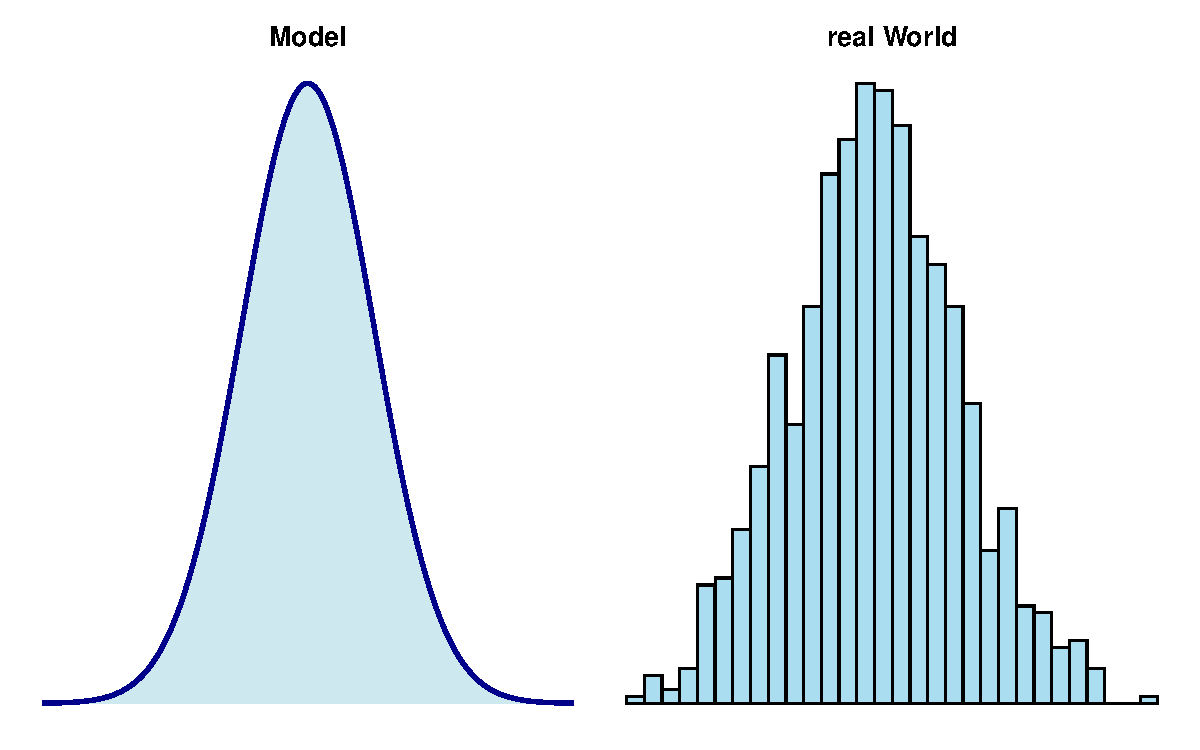
\includegraphics[width=0.95\linewidth,height=\textheight,keepaspectratio]{chapter001_Distributions_files/figure-pdf/fig-intro-1.pdf}

}

\caption{\label{fig-intro}The model is perfect, but the real world is
not.}

\end{figure}%

\section{Types of data}\label{types-of-data}

\begin{figure}[H]

\centering{

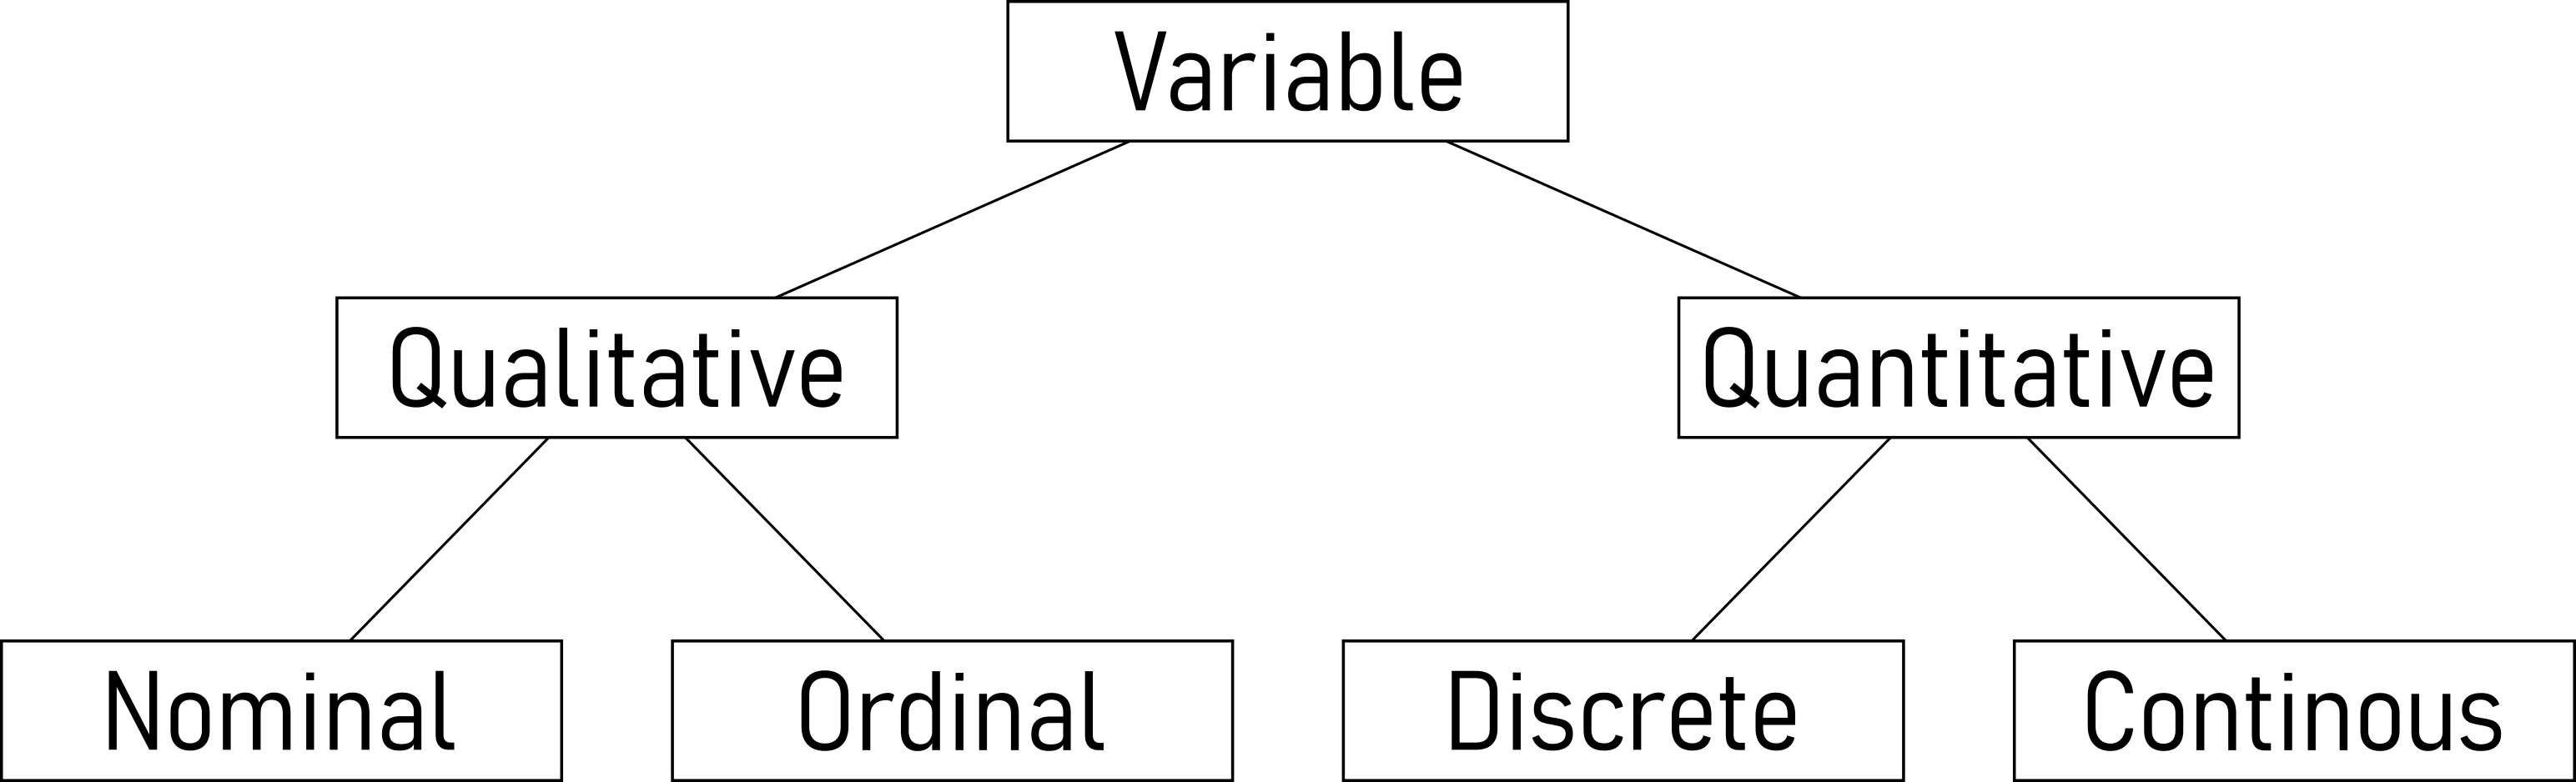
\includegraphics[width=0.95\linewidth,height=\textheight,keepaspectratio]{chapter001/013_DataTypes.png}

}

\caption{\label{fig-datatypes}Data can be classified as different
types.}

\end{figure}%

\begin{enumerate}
\def\labelenumi{\arabic{enumi}.}
\tightlist
\item
  \textbf{Nominal Data:}

  \begin{itemize}
  \tightlist
  \item
    Description: Nominal data represents categories with no inherent
    order or ranking.
  \item
    Examples: Colors, gender, or types of fruits.
  \item
    Characteristics: Categories are distinct, but there is no meaningful
    numerical value associated.
  \end{itemize}
\item
  \textbf{Ordinal Data:}

  \begin{itemize}
  \tightlist
  \item
    Description: Ordinal data has categories with a meaningful order or
    ranking, but the intervals between them are not consistent or
    measurable.
  \item
    Examples: Educational levels (e.g., high school, bachelor's,
    master's), customer satisfaction ratings (e.g., low, medium, high).
  \item
    Characteristics: The order is significant, but the differences
    between categories are not precisely quantifiable.
  \end{itemize}
\item
  \textbf{Discrete Data:}

  \begin{itemize}
  \tightlist
  \item
    Description: Discrete data consists of separate, distinct values,
    often counted in whole numbers and with no intermediate values
    between them.
  \item
    Examples: Number of students in a class, number of cars in a parking
    lot.
  \item
    Characteristics: The data points are distinct and separate; they do
    not have infinite possible values within a given range.
  \end{itemize}
\item
  \textbf{Continuous Data:}

  \begin{itemize}
  \tightlist
  \item
    Description: Continuous data can take any value within a given range
    and can be measured with precision.
  \item
    Examples: Height, weight, temperature.
  \item
    Characteristics: Values can be any real number within a range, and
    there are theoretically infinite possible values within that range.
  \end{itemize}
\end{enumerate}

\subsection{Nominal Data}\label{nominal-data}

\begin{figure}[ht]

\centering{

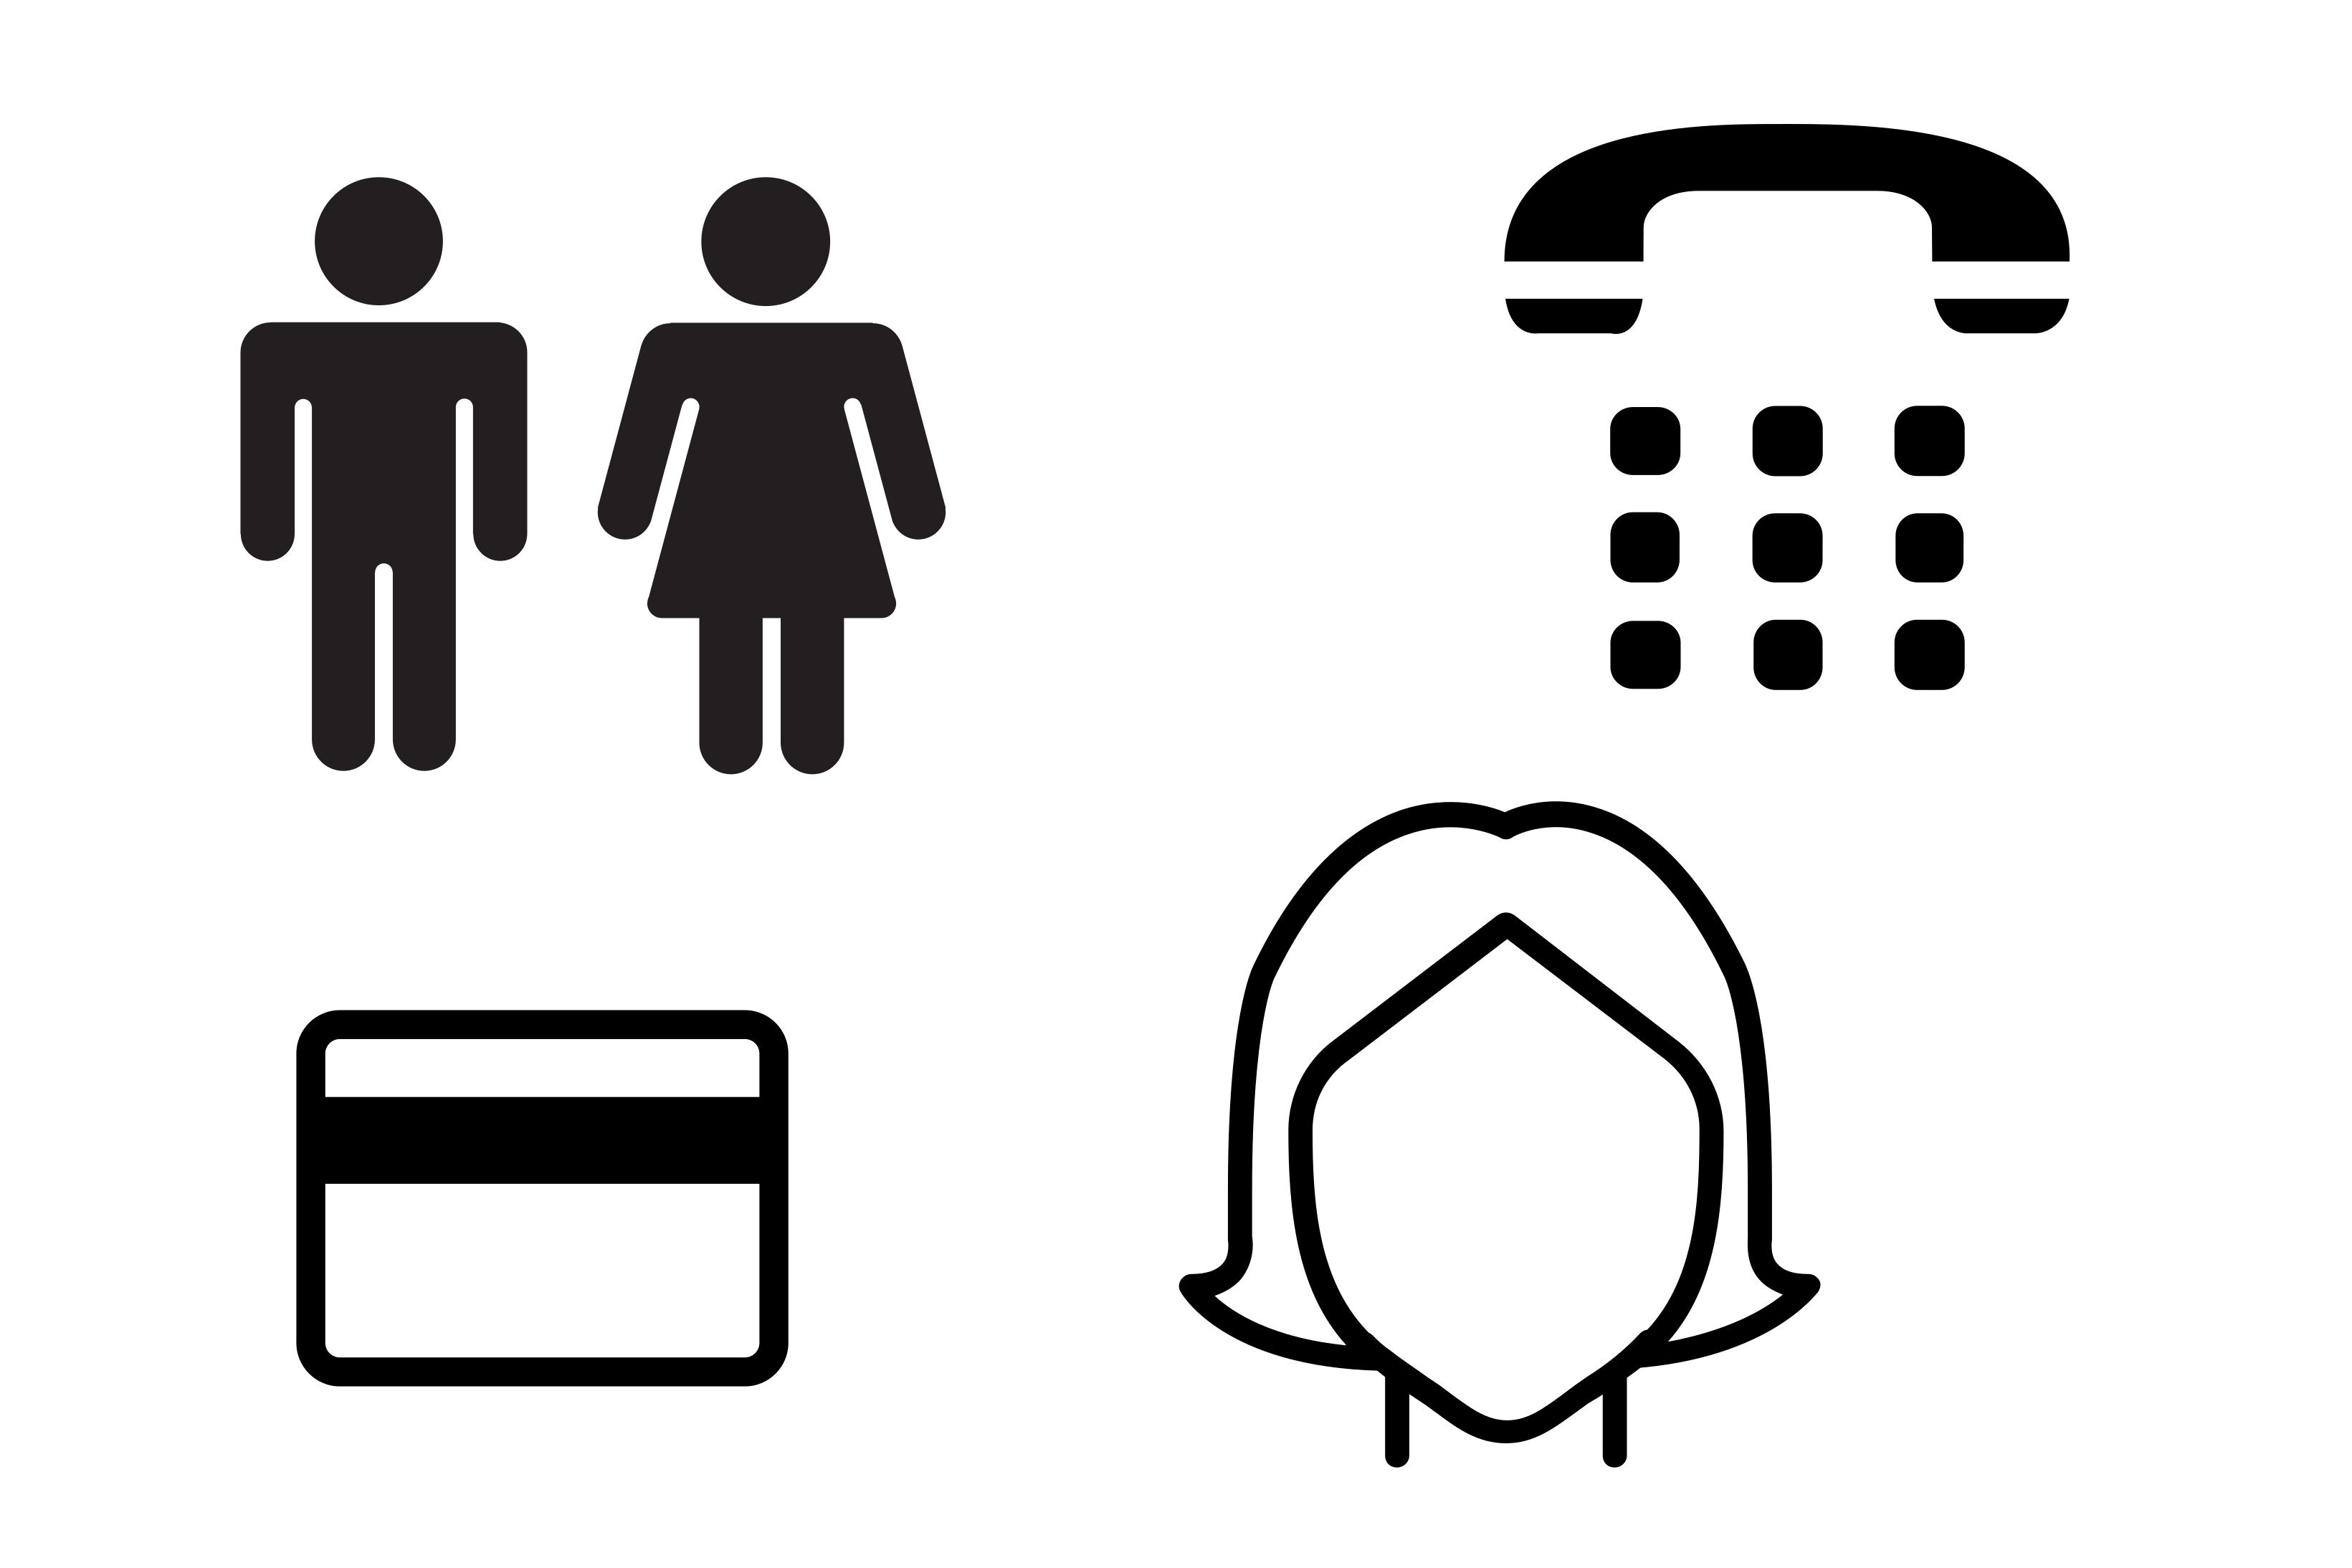
\includegraphics[width=0.95\linewidth,height=\textheight,keepaspectratio]{chapter001/014_NominalData.png}

}

\caption{\label{fig-nomialdata}Some example for nominal data.}

\end{figure}%

Nominal data is a type of data that represents categories or labels
without any specific order or ranking. These categories are distinct and
non-numeric. For example, colors, types of fruits, or gender (male,
female, other) are nominal data. Nominal data can be used for
classification and grouping, but mathematical operations like addition
or subtraction do not make sense in this context.

\subsection{Ordinal Data}\label{ordinal-data}

\begin{figure}[ht]

\centering{

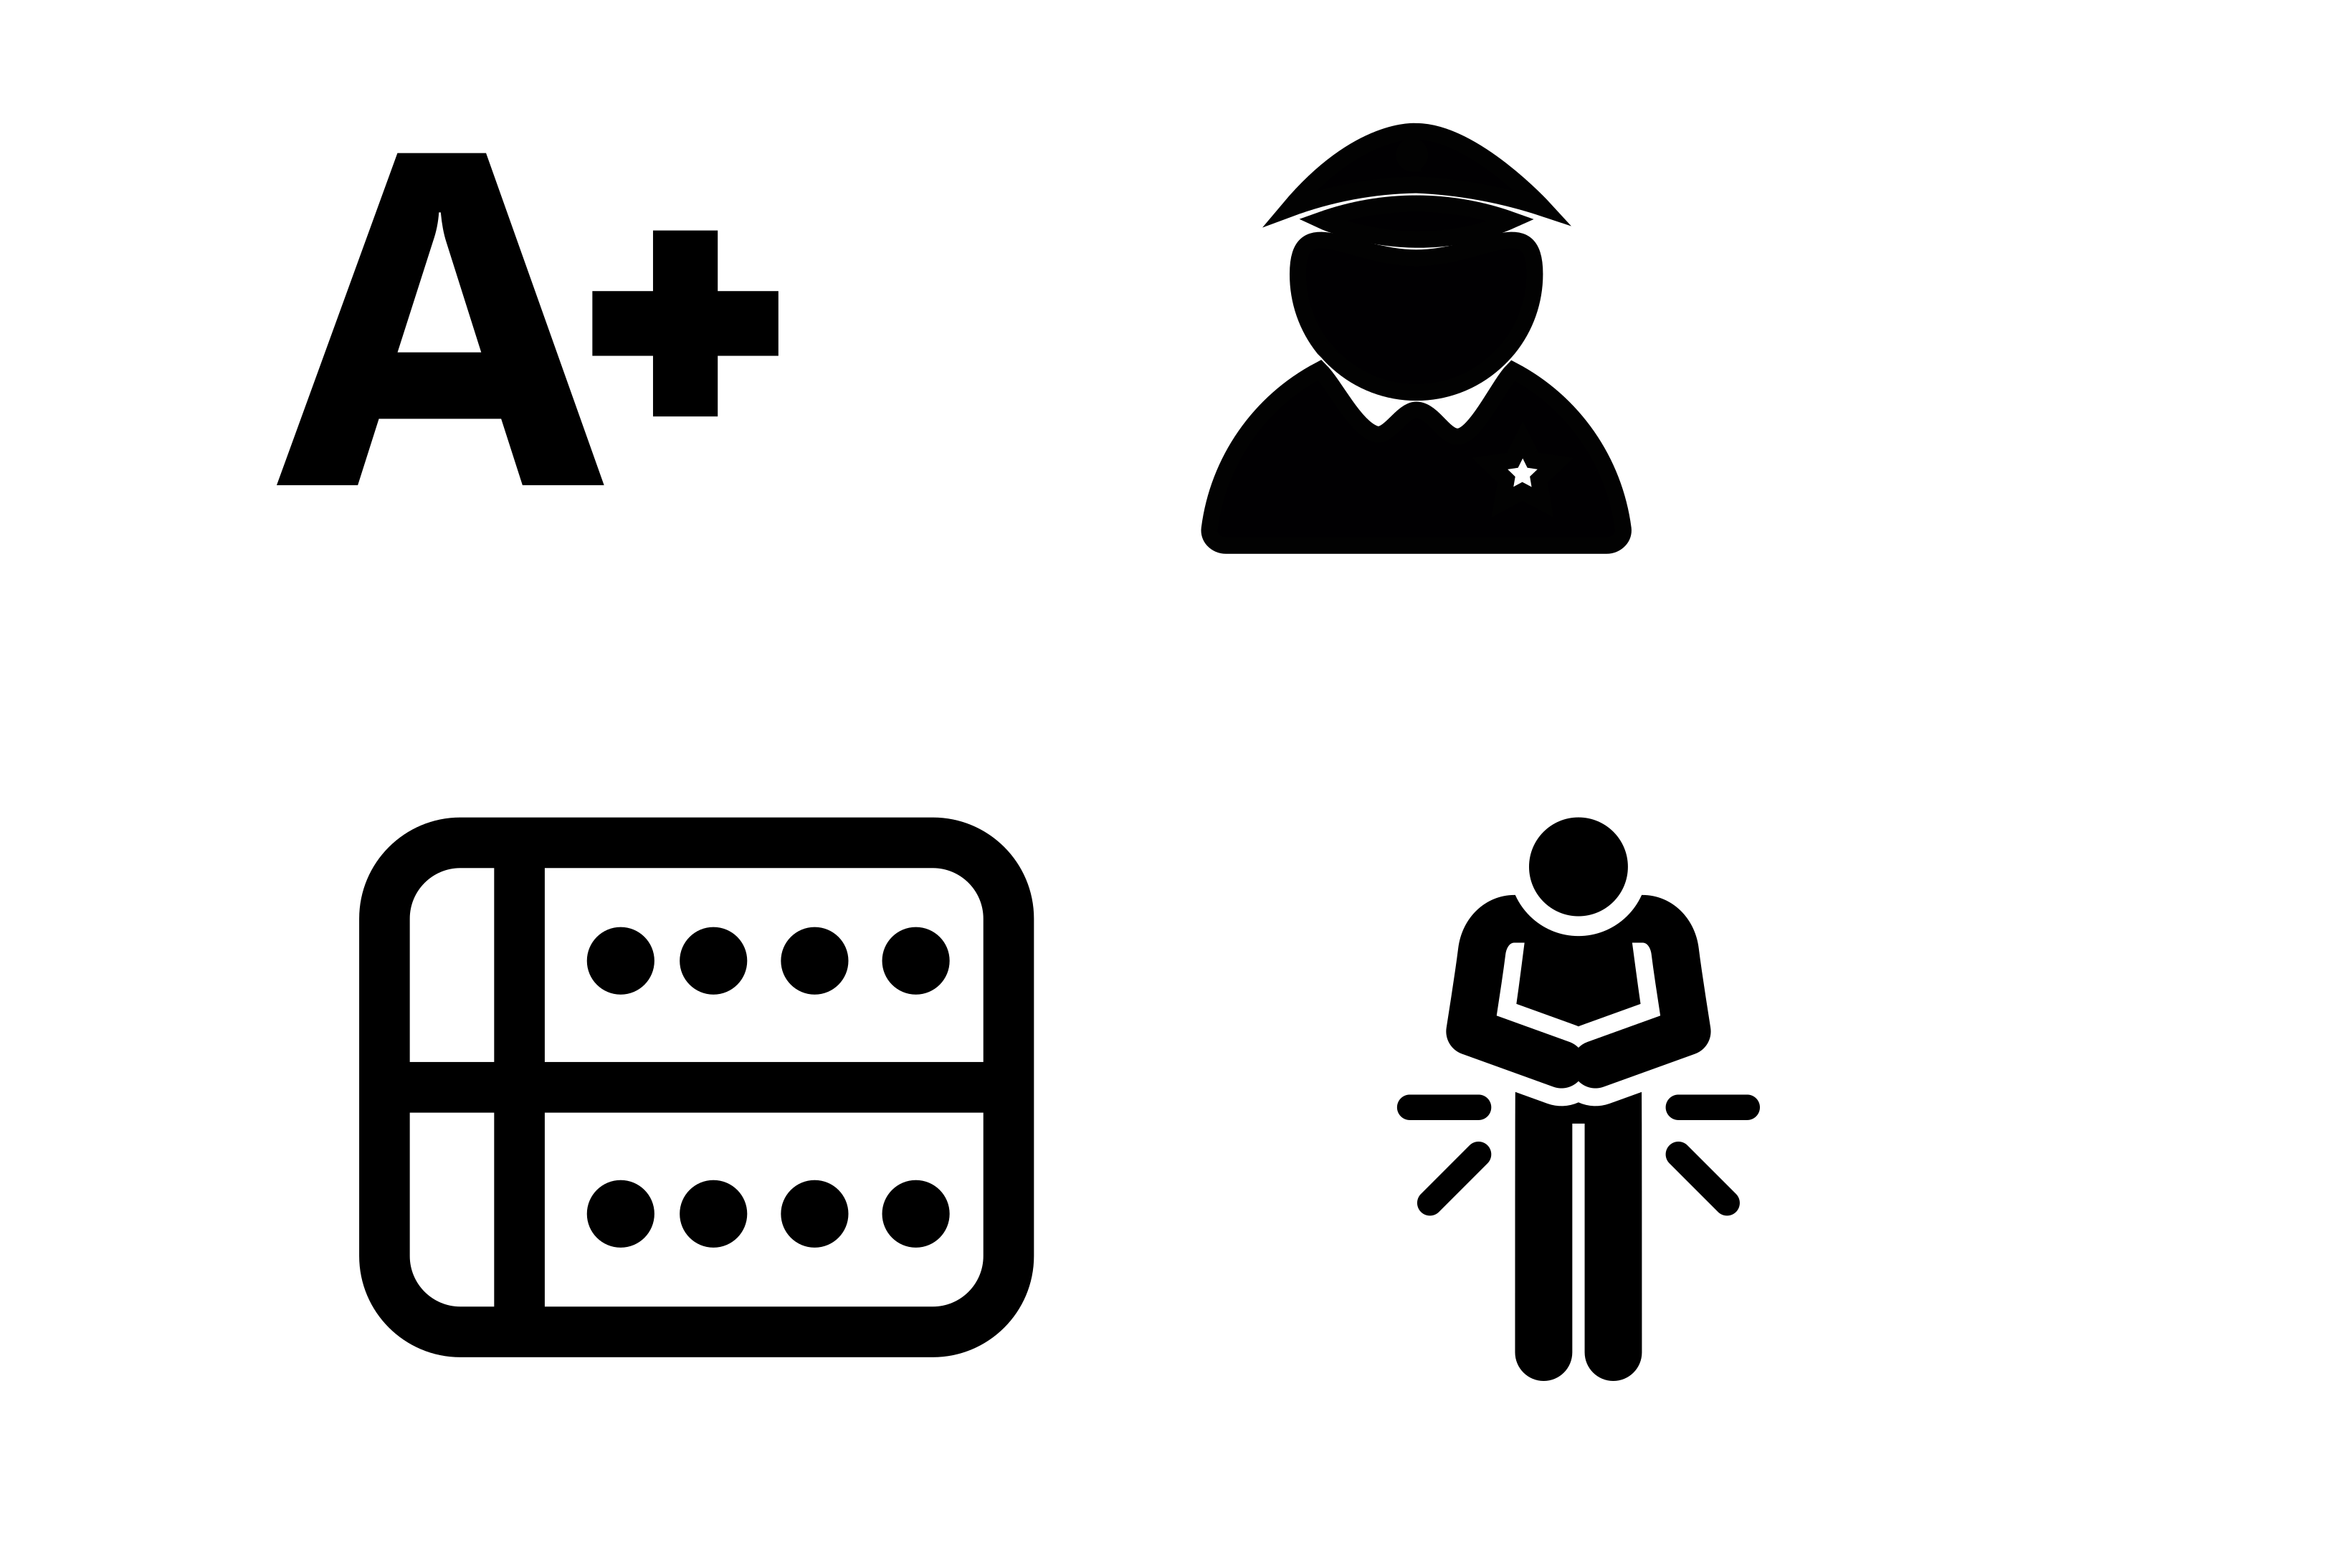
\includegraphics[width=0.95\linewidth,height=\textheight,keepaspectratio]{chapter001/015_OrdinalData.png}

}

\caption{\label{fig-ordinaldata}Some example for ordinal data.}

\end{figure}%

Ordinal data represents categories that have a specific order or
ranking. While the categories themselves may not have a consistent
numeric difference between them, they can be arranged in a meaningful
sequence. A common example of ordinal data is survey responses with
options like ``strongly agree,'' ``agree,'' ``neutral,'' ``disagree,''
and ``strongly disagree.'' These categories indicate a level of
agreement, but the differences between them may not be uniform or
measurable.

\subsection{Discrete Data}\label{discrete-data}

\begin{figure}[ht]

\centering{

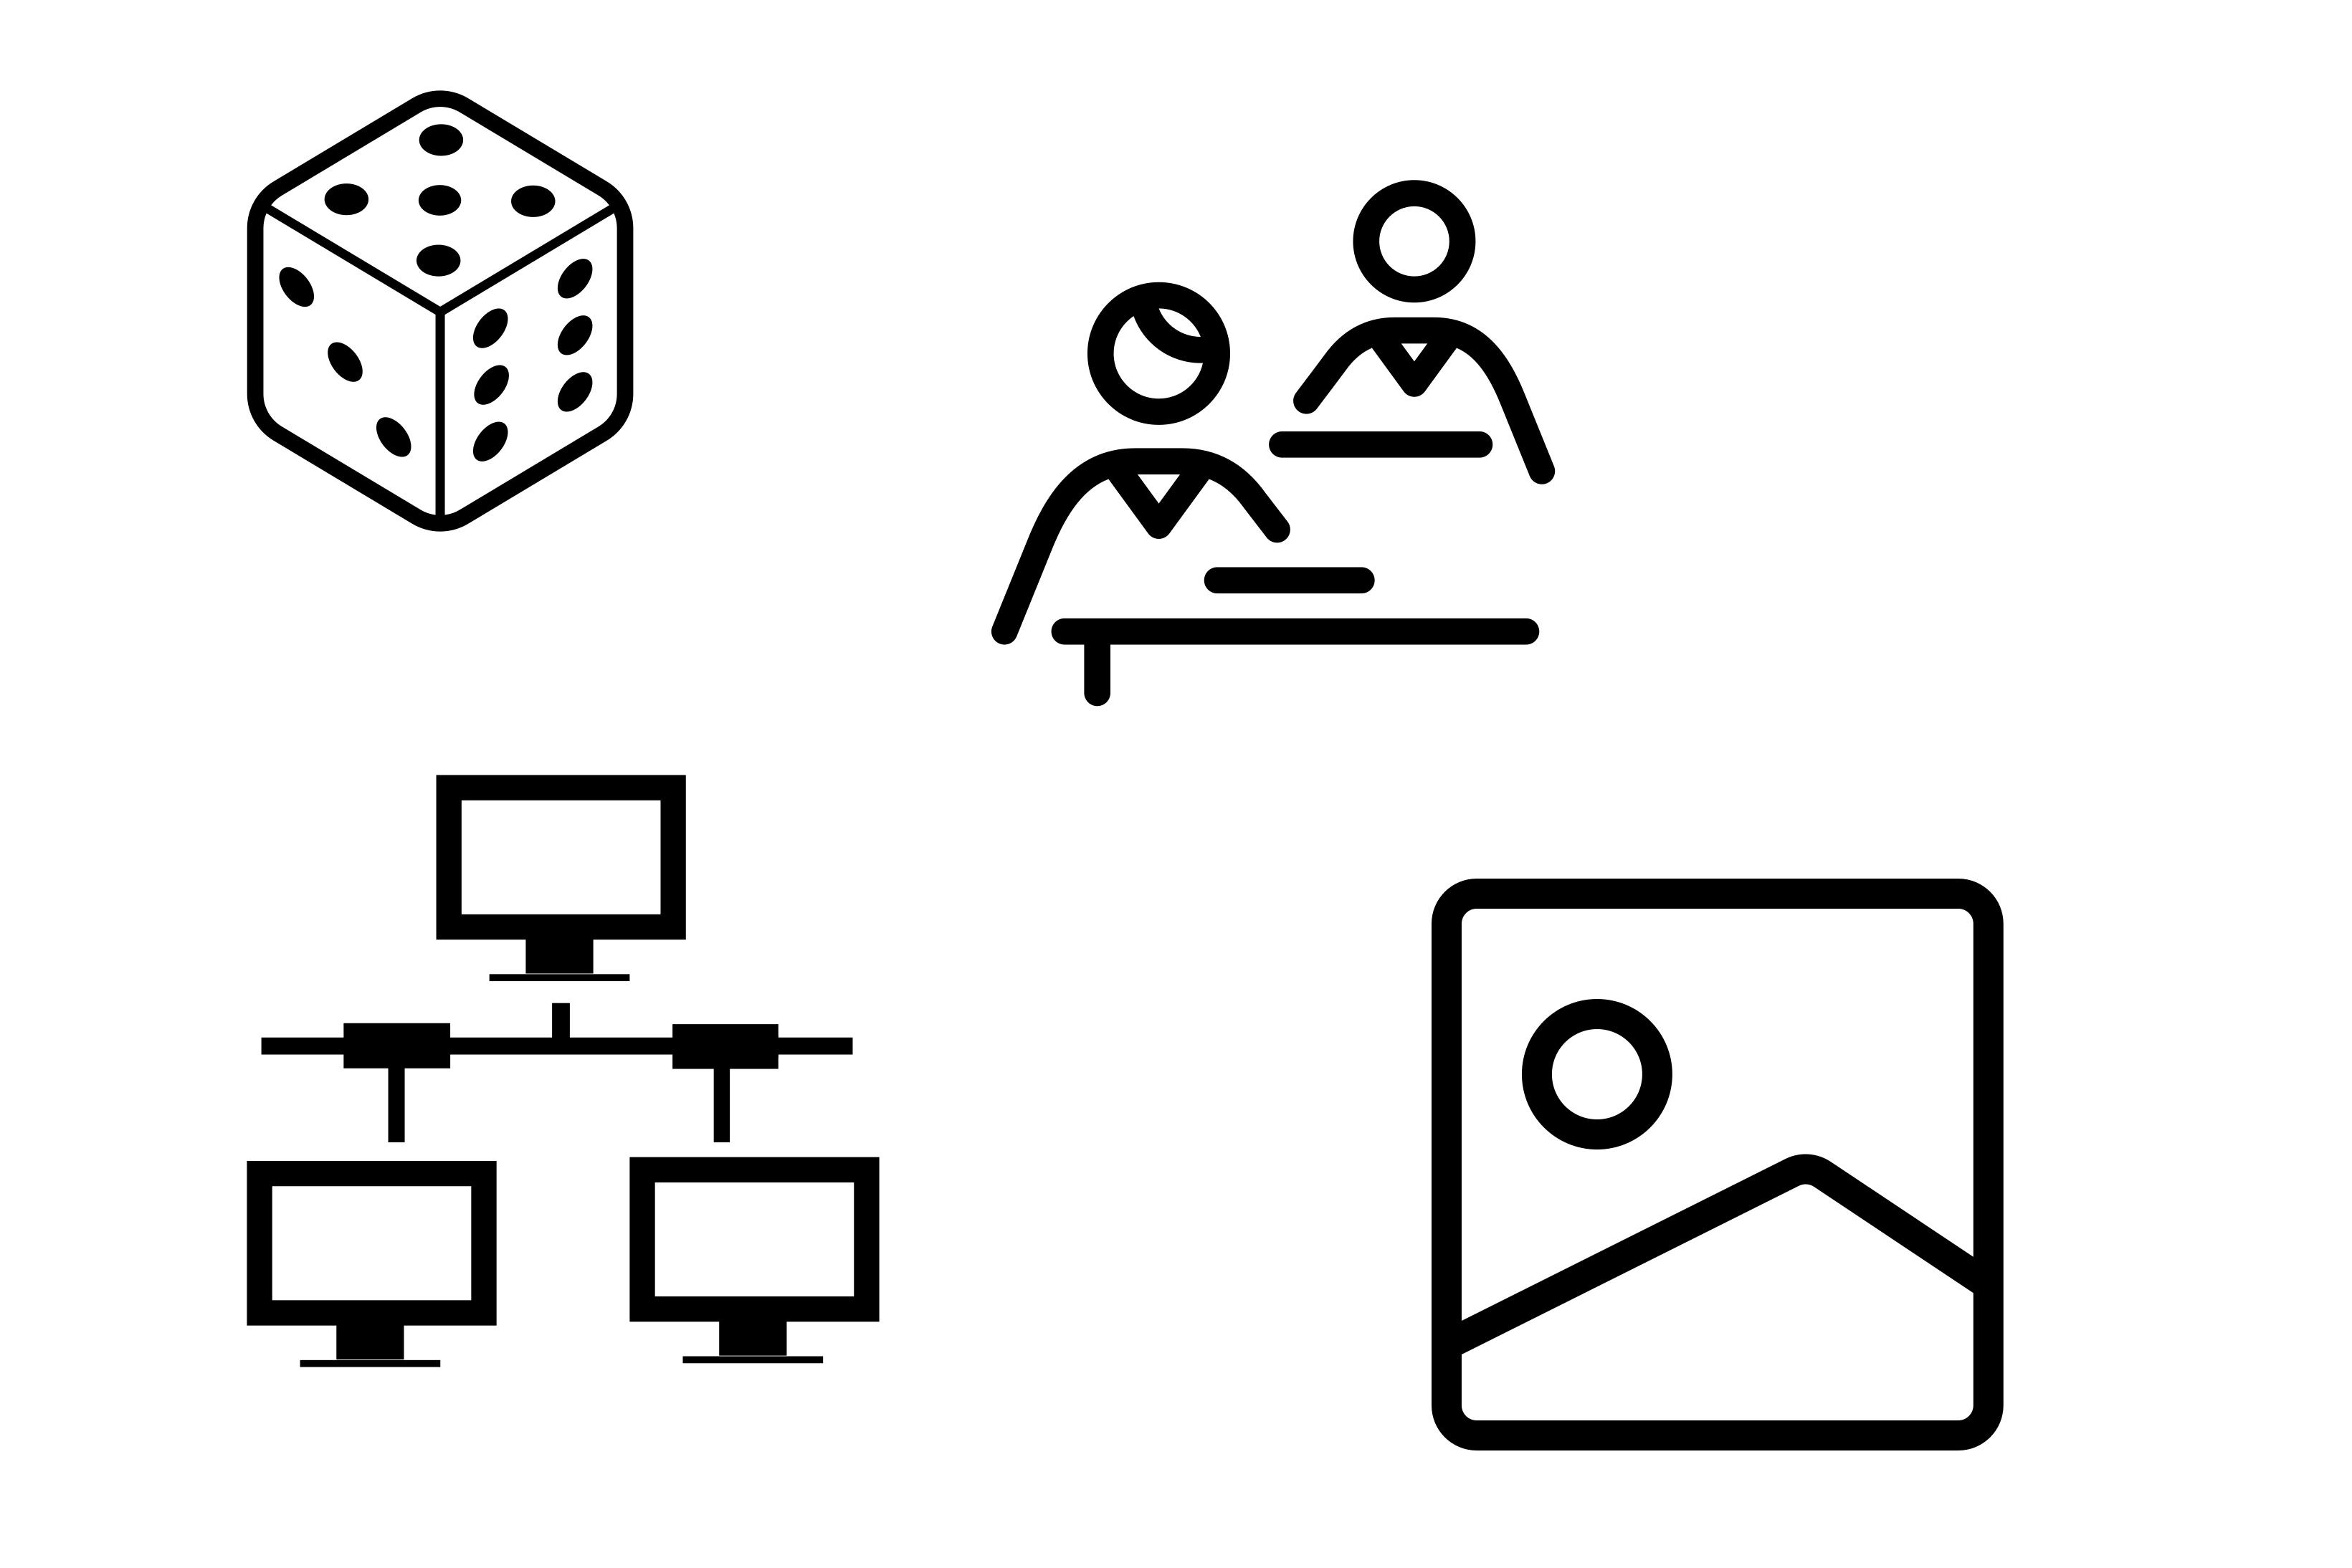
\includegraphics[width=0.95\linewidth,height=\textheight,keepaspectratio]{chapter001/016_DiscreteData.png}

}

\caption{\label{fig-discretedata}Some example for discrete data.}

\end{figure}%

Discrete data consists of distinct, separate values that can be counted
and usually come in whole numbers. These values can be finite or
infinite, but they are not continuous. Examples include the number of
students in a class, the count of cars in a parking lot, or the quantity
of books in a library. Discrete data is often used in counting and can
be represented as integers.

One quote in the literature about discrete data, shows how difficult the
classification of data types can become (J. Bibby (1980)): ``\ldots{}
All actual sample spaces are discrete, and all observable random
variables have discrete distributions. The continuous distribution is a
mathematical construction, suitable for mathematical treatment, but not
practically observable. \ldots{}''

\subsection{Continous Data}\label{continous-data}

\begin{figure}[ht]

\centering{

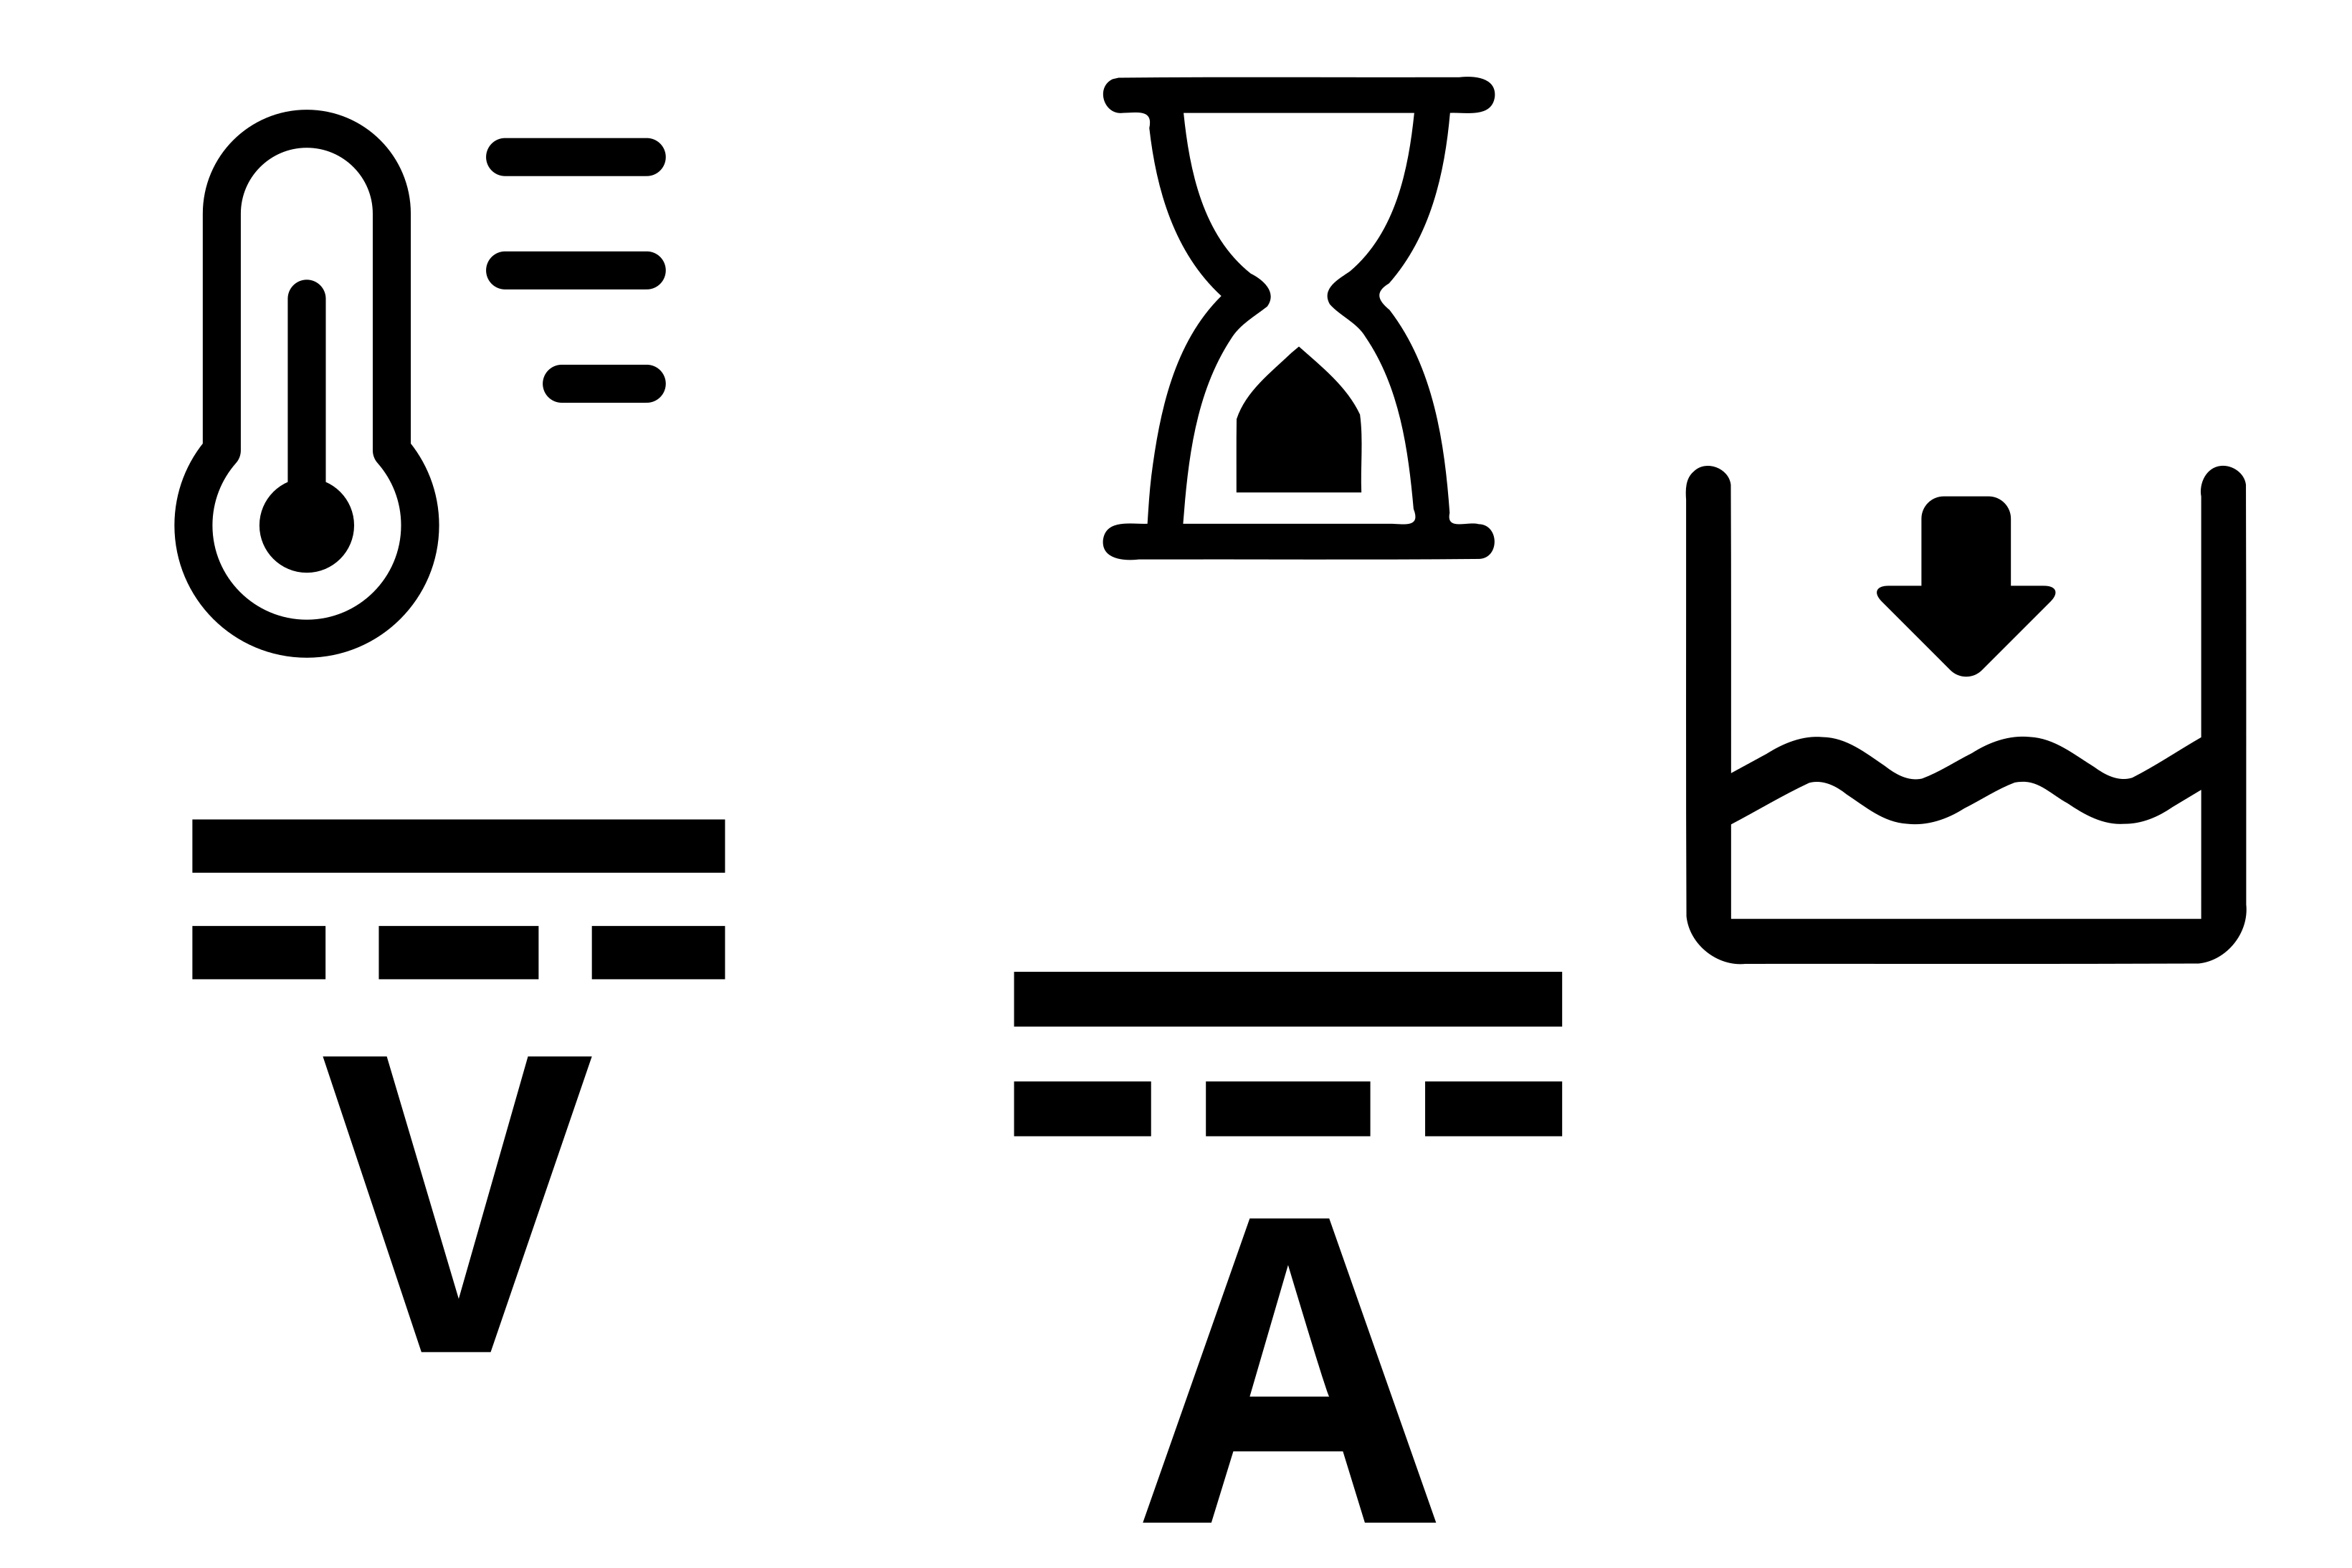
\includegraphics[width=0.95\linewidth,height=\textheight,keepaspectratio]{chapter001/017_ContinousData.png}

}

\caption{\label{fig-continousdata}Some example for continous data.}

\end{figure}%

Continuous data encompasses a wide range of values within a given
interval and can take on any real number. There are infinite
possibilities between any two points in a continuous dataset, making it
suitable for measurements with high precision. Examples of continuous
data include temperature, height, weight, and time. It is important to
note that continuous data can be measured with decimals or fractions and
is not limited to whole numbers.

\section{Uniform Distribution}\label{uniform-distribution}

\subsection{Dice}\label{dice}

\begin{figure}[ht]

\centering{

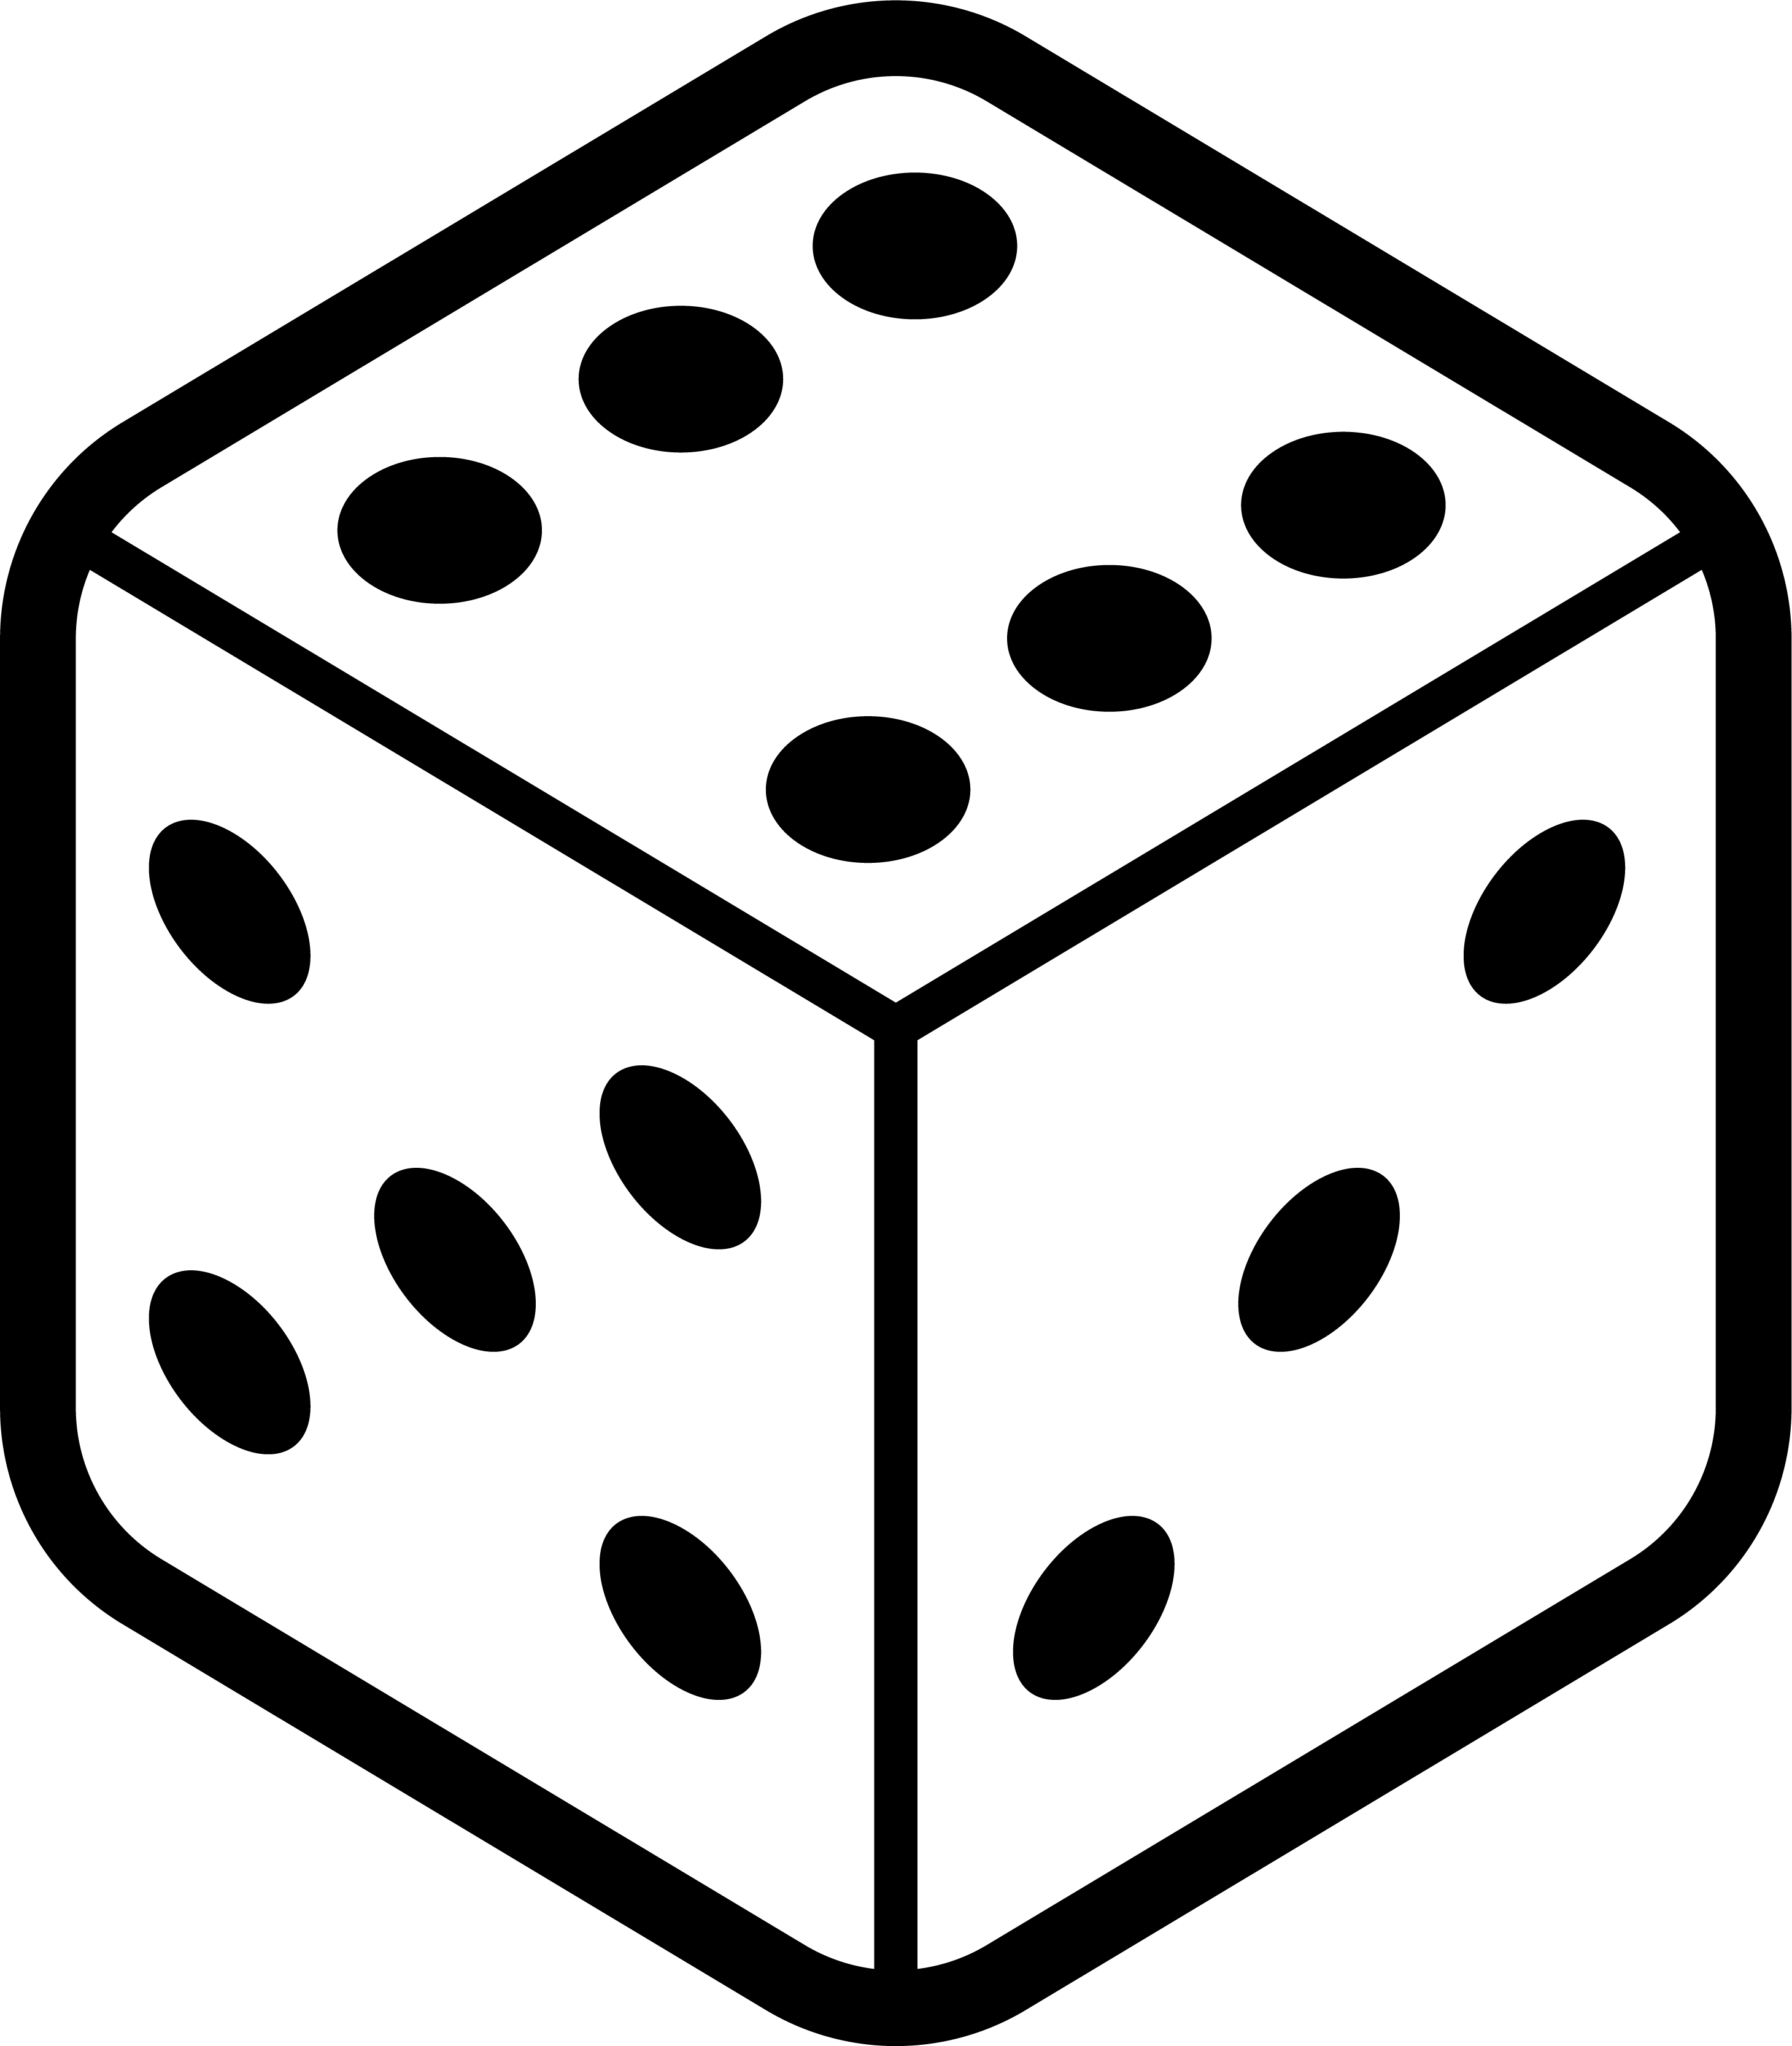
\includegraphics[width=0.35\linewidth,height=\textheight,keepaspectratio]{chapter001/die.png}

}

\caption{\label{fig-unif-die}The probability for every face to turn up
during a roll is uniformly distributed.}

\end{figure}%

\begin{figure}[ht]

\centering{

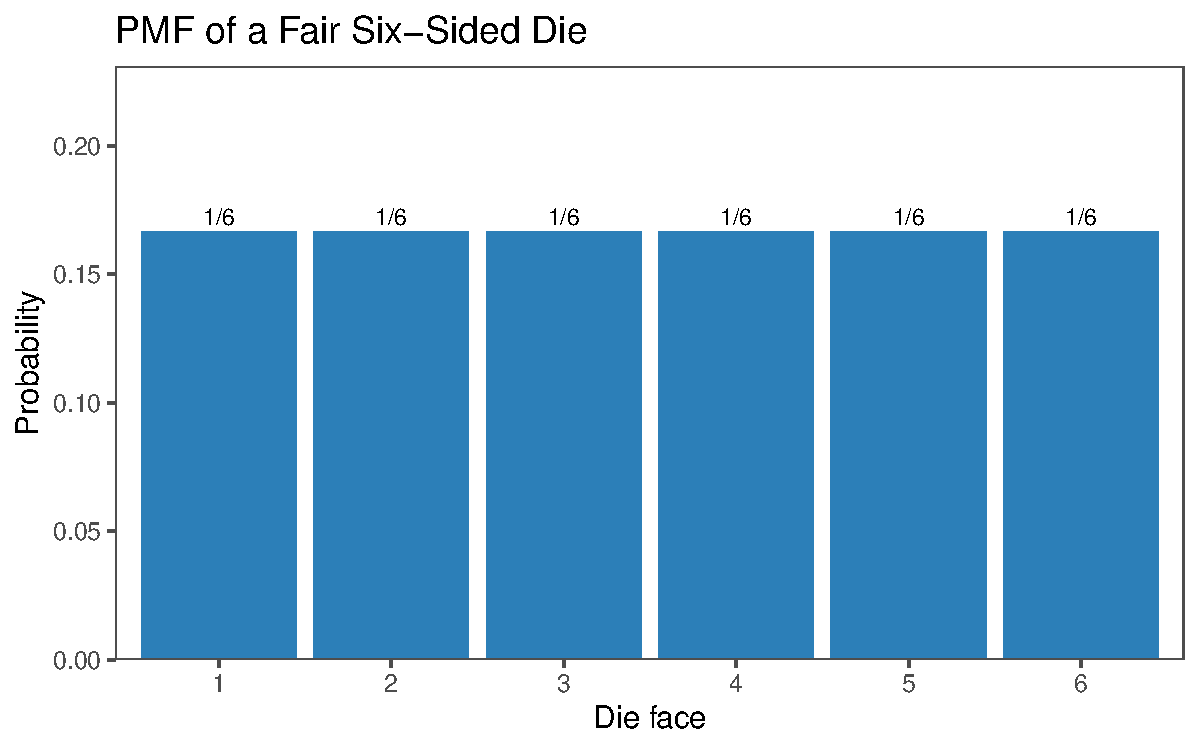
\includegraphics[width=0.95\linewidth,height=\textheight,keepaspectratio]{chapter001_Distributions_files/figure-pdf/fig-unif-pmf-1.pdf}

}

\caption{\label{fig-unif-pmf}A plot of the probabilities that every face
of a die turns up. They are all the same.}

\end{figure}%

\subsection{Types of uniform
distributions}\label{types-of-uniform-distributions}

\begin{itemize}
\tightlist
\item
  All outcomes in the range are \emph{equally probable}
\item
  The ``range'' can be:

  \begin{itemize}
  \tightlist
  \item
    a finite set of values (discrete)
  \item
    a continuous interval (continuous)
  \end{itemize}
\end{itemize}

\begin{align}
X \sim \mathrm{Uniform}(a,b) \text{ continuous}\\
X \sim \mathrm{Uniform}\{a,a+1,\ldots,b\} \text{ discrete}
\end{align}

\subsection{Visual comparison of discrete and
continuous}\label{visual-comparison-of-discrete-and-continuous}

\begin{figure}[ht]

\centering{

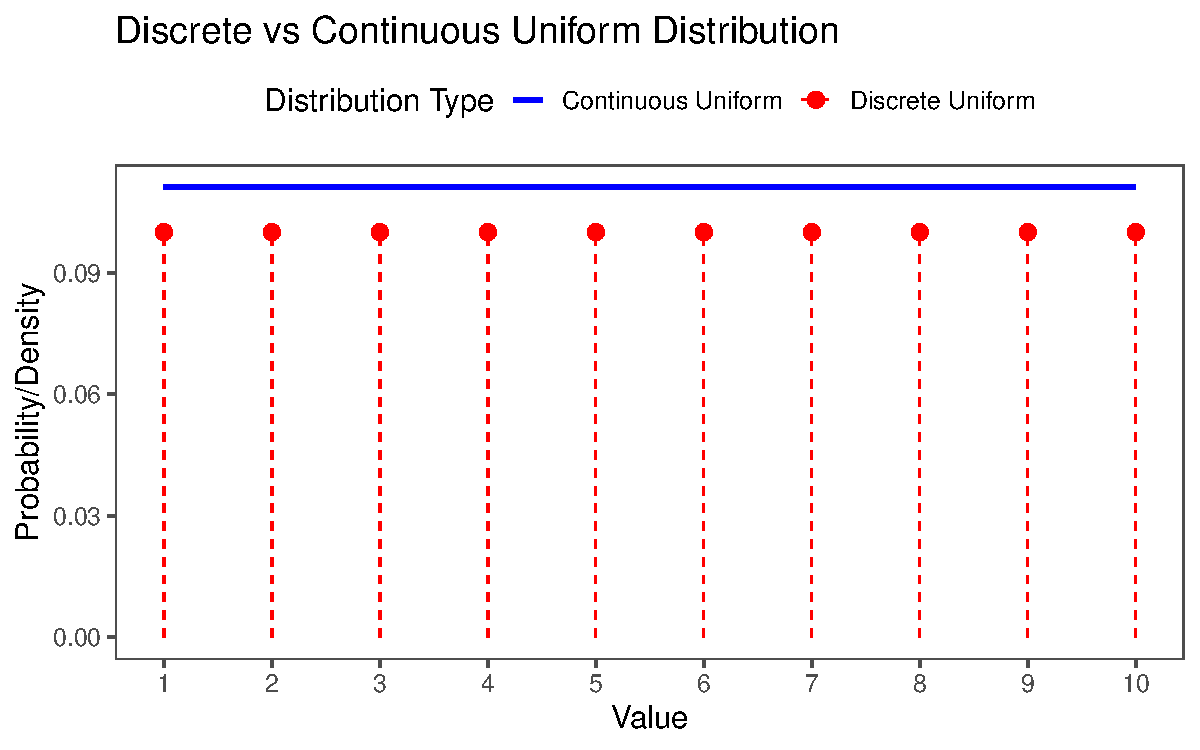
\includegraphics[width=0.95\linewidth,height=\textheight,keepaspectratio]{chapter001_Distributions_files/figure-pdf/fig-unif-pmf-pdf-1.pdf}

}

\caption{\label{fig-unif-pmf-pdf}A comparison of continnuous and
discrete uniformly distributed data.}

\end{figure}%

\subsection{Core properties}\label{core-properties}

\begin{table}

\caption{\label{tbl-unif-prop}The core properties between the discrete
and continuous disitrbution are very similar.}

\centering{

\caption*{
{\fontsize{14}{17}\selectfont  \textbf{Core Properties: Discrete vs. Continuous Uniform Distributions}\fontsize{12}{15}\selectfont } \\ 
{\fontsize{12}{15}\selectfont  \emph{Equal probability everywhere, but for different types of data}\fontsize{12}{15}\selectfont }
} 
\fontsize{12.0pt}{14.0pt}\selectfont
\begin{tabular*}{\linewidth}{@{\extracolsep{\fill}}lll}
\toprule
\textbf{Property} & \textbf{Discrete Uniform} & \textbf{Continuous Uniform} \\ 
\midrule\addlinespace[2.5pt]
{Probability} & {\cellcolor[HTML]{F0F0F0}{Equal for each outcome.}} & {\cellcolor[HTML]{E6F3FF}{Equal density over the interval.}} \\ 
{Symmetry} & {\cellcolor[HTML]{F0F0F0}{Mean = midpoint of the range.}} & {\cellcolor[HTML]{E6F3FF}{Mean = midpoint of the interval.}} \\ 
{Intuition} & {\cellcolor[HTML]{F0F0F0}{`Fair die' with n sides.}} & {\cellcolor[HTML]{E6F3FF}{`Fair spinner' on a line segment.}} \\ 
{Use Cases} & {\cellcolor[HTML]{F0F0F0}{Counting problems (e.g., dice, cards).}} & {\cellcolor[HTML]{E6F3FF}{Measuring problems (e.g., time, space).}} \\ 
\bottomrule
\end{tabular*}
\begin{minipage}{\linewidth}
\emph{Note: Both distributions share the `fairness' property but apply to different data types.}\\
\end{minipage}

}

\end{table}%

\section{\texorpdfstring{\hyperref[acronyms_PMF]{Probability Mass
Function (PMF)}}{Probability Mass Function (PMF)}}\label{section-2}

\subsection{But why?}\label{but-why}

\begin{itemize}
\tightlist
\item
  \hyperref[acronyms_PMF]{PMF}s provide a way to calculate and assign
  probabilities to each distinct outcome.
\item
  Each outcome is assigned a probability that corresponds to its
  position in the total number of outcomes.
\end{itemize}

\subsection{Basics}\label{basics}

\ldots{} assigns each outcome the same probability that always sum up to
\(1\) (example: six-sided die)

\(X \sim \mathrm{Uniform}\{a,b\}\) where \(a\) and \(b\) are integers
and \(a\leq b\)

\begin{align}
f(k) = P (X = k)
\end{align}

\begin{itemize}
\tightlist
\item
  \(k\) meaning a specific value that \(X\) can take (e.g.,
  \(k = 0,1,2, ...\))
\item
  \(f(k)\) is the probability that \(X\) equals \(k\)
\end{itemize}

\subsection{Key Properties}\label{key-properties}

\begin{enumerate}
\def\labelenumi{\arabic{enumi}.}
\tightlist
\item
  \(0 \leq f(k) \leq 1\) for all \(k\)
\item
  The of probabilities over all possible \(k\) must equal \(1\)
\end{enumerate}

\begin{align}
\sum_{all \; k}f(k) = 1
\end{align}

\subsection{6-sided die}\label{sided-die}

\begin{align}
X &\sim \mathrm{Uniform}\{a,a+1, ..., b\} \\
X &\sim \mathrm{Uniform}\{1,2,3,4,5,6\}
\end{align}

Number of outcomes:

\begin{align}
N &= b-a+1\\
N &= 6-1+1=6
\end{align}

Equal probability for each outcome: \(f(k) = P (X = k)\)

\begin{align}
f(a) = f(a+1)= ... = f(b) = c \text{ (some constant)}
\end{align}

\begin{center}\rule{0.5\linewidth}{0.5pt}\end{center}

Sum of all probabilities must equal 1

\begin{align}
\sum_{k = a}^b f(k) = \underbrace{c+c+ ... +}_{N\text{times}} = N \cdot c = 1
\end{align}

Solving for \(c\)

\begin{align}
c = \frac{1}{N} = \frac{1}{b-a+1}
\end{align}

\begin{center}\rule{0.5\linewidth}{0.5pt}\end{center}

Formal \hyperref[acronyms_PMF]{PMF}:

\begin{align}
f(k) = \begin{cases}
\frac{1}{b - a + 1} & \text{if } k \in \{a, a+1, \dots, b\}, \\
0 & \text{otherwise.}
\end{cases}
\end{align}

\subsection{Exercise}\label{exercise}

A tool changer in production randomly selects one of four tools (labeled
1 to 4) with equal probability.

\begin{itemize}
\tightlist
\item
  Describe the formal set in \(X \sim ...\)
\end{itemize}

\(X \sim \mathrm{Uniform}\{1,2,3,4\}\)

\begin{itemize}
\tightlist
\item
  Formally calculate the number of outcomes (\(N\))
\end{itemize}

\(N = 4-1+1 = 4\)

\begin{center}\rule{0.5\linewidth}{0.5pt}\end{center}

\begin{itemize}
\tightlist
\item
  Describe the \hyperref[acronyms_PMF]{PMF} formally
\end{itemize}

\begin{align}
f(k) = \begin{cases}
\frac{1}{4} & \text{if } k \in \{1,2,3,4\}, \\
0 & \text{otherwise.}
\end{cases}
\end{align}

\begin{itemize}
\tightlist
\item
  What is the probability to select tool \(2\)
\end{itemize}

\(P(X = 2) = f(2) = \frac{1}{4} = 0.25\)

\subsection{\texorpdfstring{Summary
\hyperref[acronyms_PMF]{PMF}}{Summary PMF}}\label{summary}

\begin{itemize}
\item
  The \hyperref[acronyms_PMF]{PMF} describes the probability
  distribution of a discrete random variable.
\item
  The probabilities associated with all hypothetical values must be
  non-negative and sum up to 1.
\item
  A \hyperref[acronyms_PMF]{PMF} is specific to \emph{discrete} random
  variables, while a \hyperref[acronyms_PDF]{PDF} is associated with
  continuous random variables.
\item
  Unlike a PDF, which requires integration over an interval, the PMF
  \textbf{directly} provides probabilities for individual values.
\item
  ``mass'' is conserved (similar to how physical mass is conserved).
\end{itemize}

\section{Binomial Distribution}\label{binomial-distribution}

\subsection{Classroom example}\label{classroom-example}

If we roll a fair six-sided die 10 times, how many times do you expect
to get a specific outcome?

\begin{itemize}
\tightlist
\item
  10 trials
\item
  \(P?\) to roll a \(6\) (expected value)?
\item
  record the number of times a specific outcome occurs
\item
  repeat for 2-4 students
\end{itemize}

\begin{itemize}
\tightlist
\item
  \(P = 1/6 \approx 16\% \rightarrow P_{10\;times} = 10 * 1/6 = 1.6 times \approx 2\)
\end{itemize}

\begin{figure}[ht]

\centering{

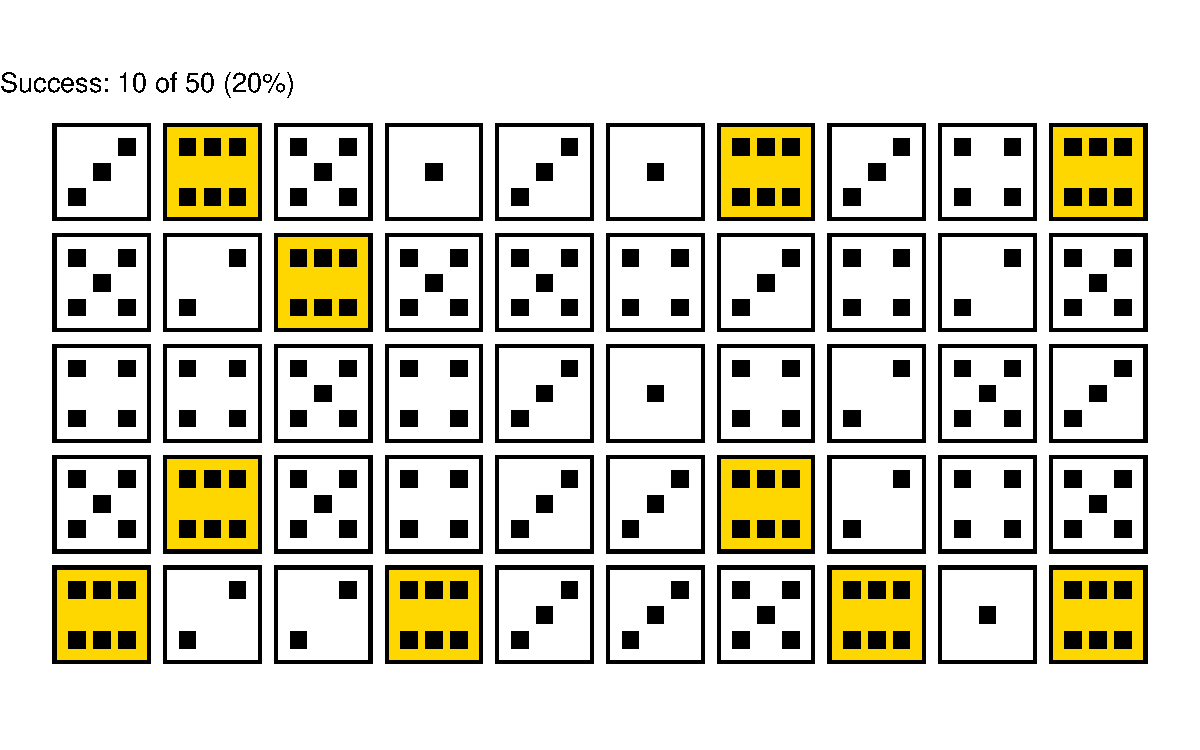
\includegraphics[width=0.75\linewidth,height=\textheight,keepaspectratio]{chapter001_Distributions_files/figure-pdf/fig-sim-dice-1.pdf}

}

\caption{\label{fig-sim-dice}Simulated die rolls (The die is rolle
\(10\) times, the experiment is repeated \(5\) times)}

\end{figure}%

\begin{figure}[ht]

\centering{

\pandocbounded{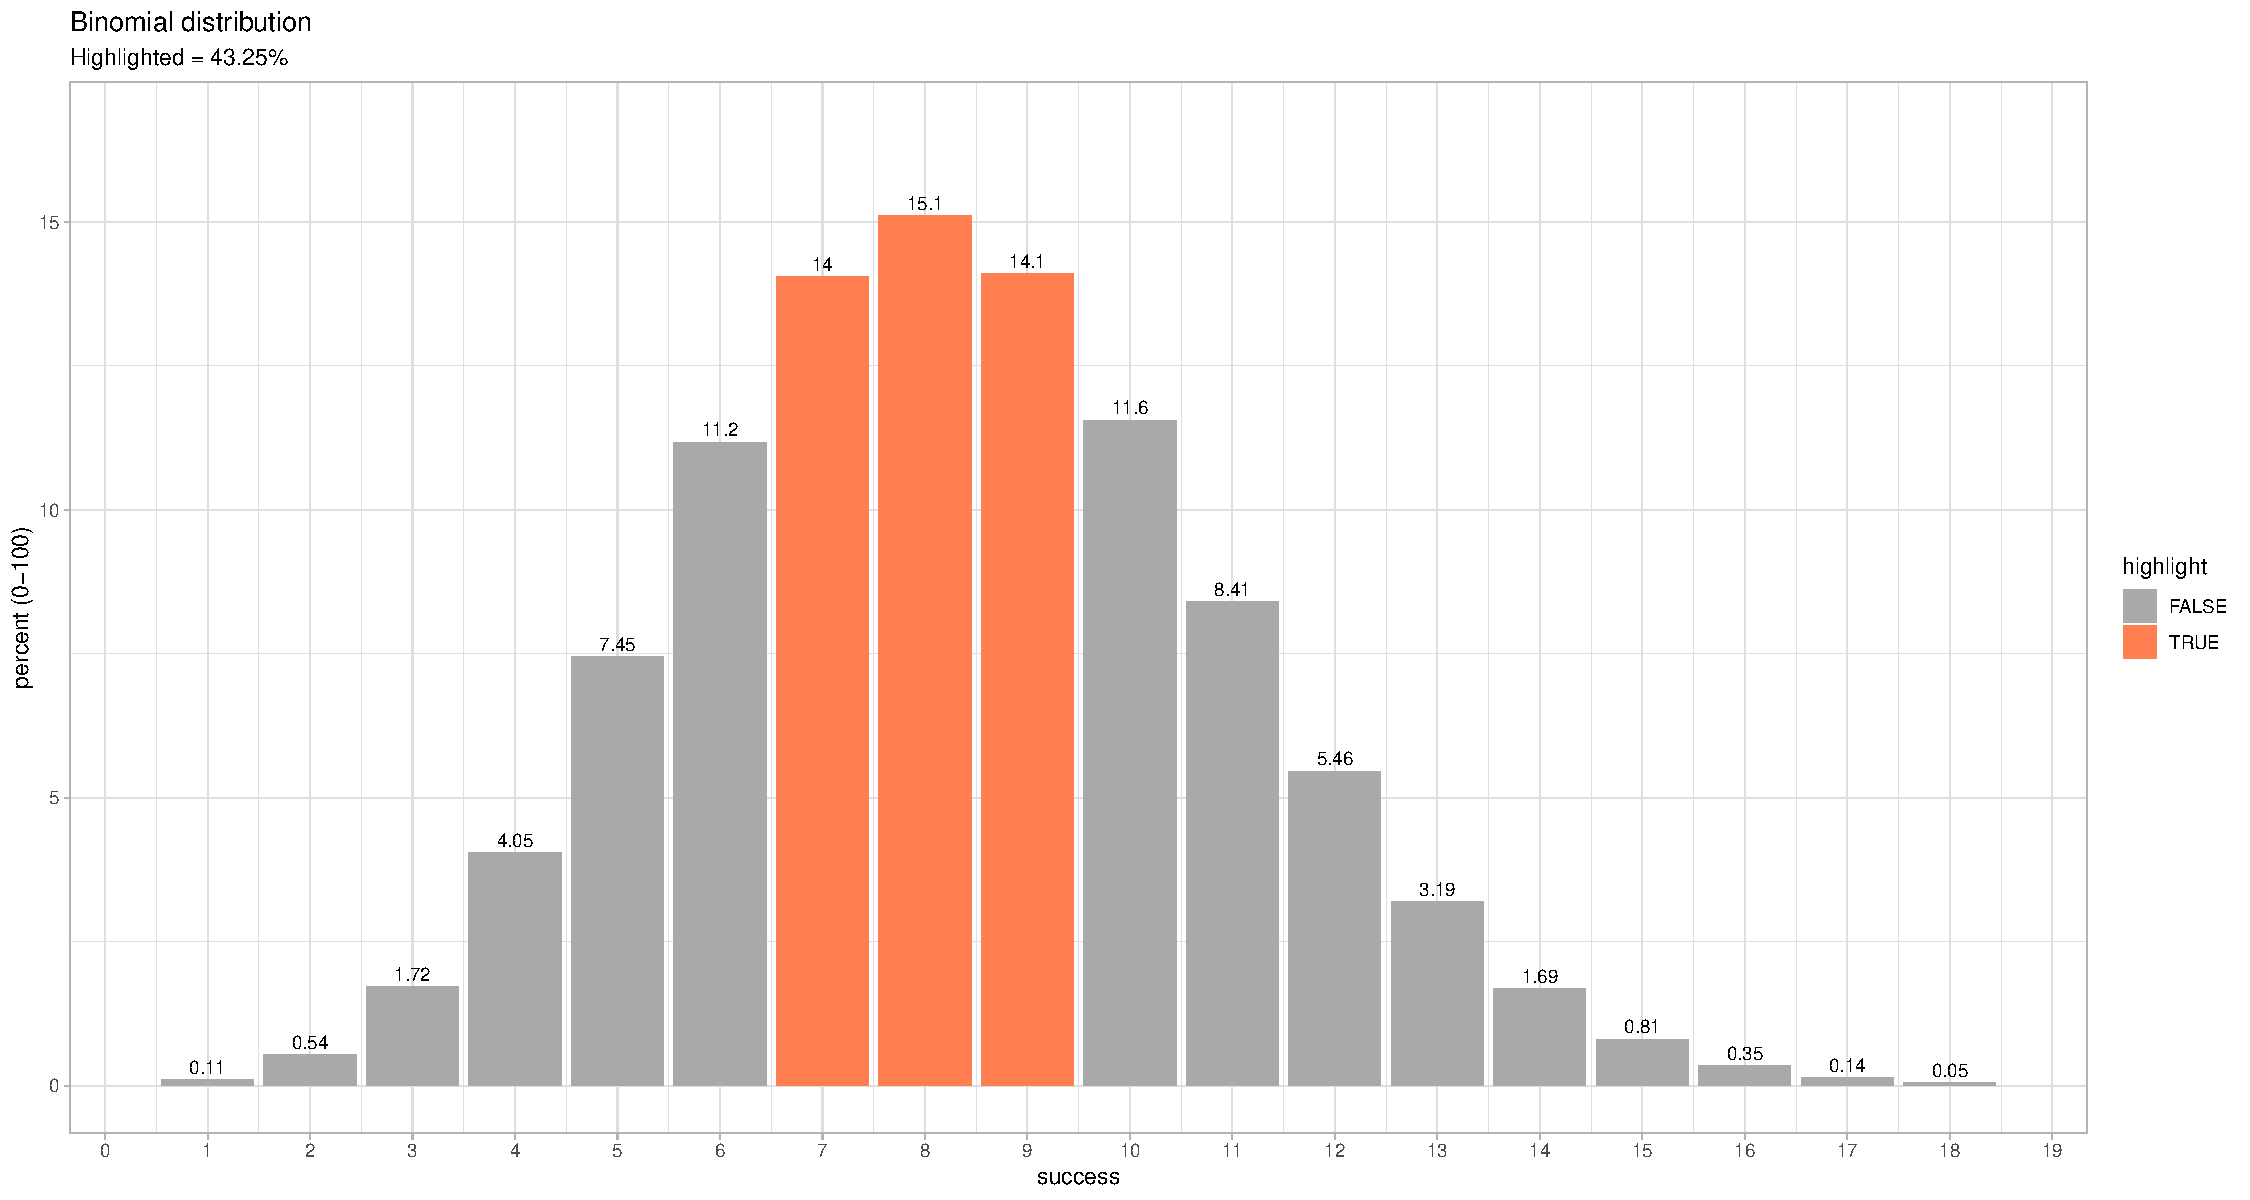
\includegraphics[keepaspectratio]{chapter001_Distributions_files/figure-pdf/fig-sim-likely-1.pdf}}

}

\caption{\label{fig-sim-likely}Is the outcome likely?}

\end{figure}%

\subsection{Theory}\label{theory}

\begin{figure}[ht]

\centering{

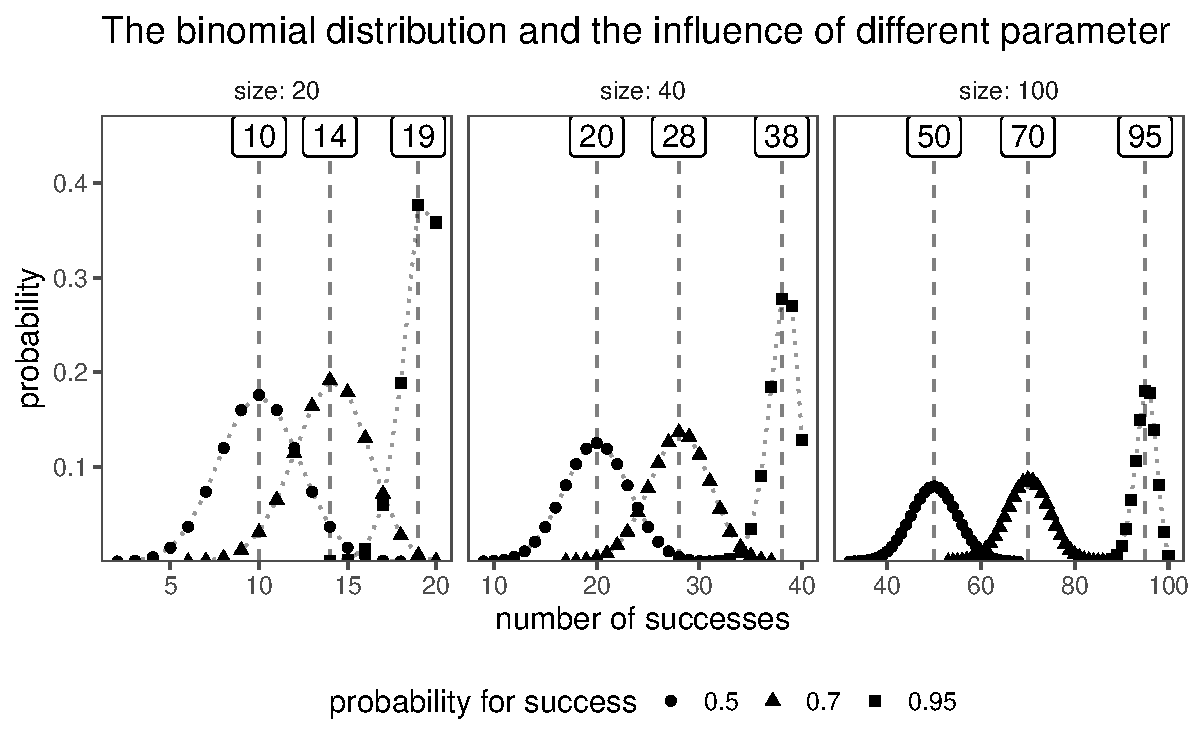
\includegraphics[width=0.95\linewidth,height=\textheight,keepaspectratio]{chapter001_Distributions_files/figure-pdf/fig-bn-dist-1.pdf}

}

\caption{\label{fig-bn-dist}The binomial distribution}

\end{figure}%

The binomial distribution is a \textbf{discrete} probability
distribution that describes the number of successes in a fixed number of
independent Bernoulli trials, each with the same probability of success.
A Bernoulli trial, named after Swiss mathematician Jacob
Bernoulli\footnote{Jacob Bernoulli (1654-1705): Notable Swiss
  mathematician, known for Bernoulli's principle and significant
  contributions to calculus and probability theory.}, is a random
experiment or trial with two possible outcomes: success and failure.
These outcomes are typically labeled as \(1\) for success and \(0\) for
failure. The key characteristics of a Bernoulli trial are:

\begin{enumerate}
\def\labelenumi{\arabic{enumi}.}
\item
  \textbf{Two Outcomes:} There are only two possible outcomes in each
  trial, and they are mutually exclusive. For example, in a coin toss,
  the outcomes could be heads (success, represented as \(1\)) or tails
  (failure, represented as \(0\)).
\item
  \textbf{Constant Probability:} The probability of success remains the
  same for each trial. This means that the likelihood of success and
  failure is consistent from one trial to the next.
\item
  \textbf{Independence:} Each trial is independent of others, meaning
  that the outcome of one trial does not influence the outcome of
  subsequent trials. For instance, the result of one coin toss doesn't
  affect the result of the next coin toss.
\end{enumerate}

Examples of Bernoulli trials include:

\begin{itemize}
\tightlist
\item
  Flipping a coin (heads as success, tails as failure).
\item
  Rolling a die and checking if a specific number appears (the number as
  success, others as failure).
\item
  Testing whether a manufactured product is defective or non-defective
  (defective as success, non-defective as failure).
\end{itemize}

The Bernoulli trial is the fundamental building block for many other
probability distributions, including the binomial distribution, which
models the number of successes in a fixed number of Bernoulli trials.

The \hyperref[acronyms_PMF]{PMF}, also known as the discrete probability
density function, is a fundamental concept in probability and
statistics.

\begin{itemize}
\item
  Definition: The \hyperref[acronyms_PMF]{PMF} describes the probability
  distribution of a discrete random variable. It gives the probability
  that the random variable takes on a specific value. In other words,
  the PMF assigns probabilities to each possible outcome of the random
  variable.
\item
  Formal Representation: For a discrete random variable X, the PMF is
  denoted as \(P(X = x)\), where \(x\) represents a specific value.
  Mathematically, the PMF is defined as:
  \(P(X = x) = \text{{probability that }} X \text{{ takes the value }} x\)
\item
  Properties: The probabilities associated with all hypothetical values
  must be non-negative and sum up to 1. Thinking of probability as
  ``mass'' helps avoid mistakes, as the total probability for all
  possible outcomes is conserved (similar to how physical mass is
  conserved).
\item
  Comparison with \hyperref[acronyms_PDF]{PDF}: A
  \hyperref[acronyms_PMF]{PMF} is specific to \emph{discrete} random
  variables, while a \hyperref[acronyms_PDF]{PDF} is associated with
  continuous random variables. Unlike a \hyperref[acronyms_PDF]{PDF},
  which requires integration over an interval, the
  \hyperref[acronyms_PMF]{PMF} \textbf{directly} provides probabilities
  for individual values.
\item
  Mode: The value of the random variable with the largest probability
  mass is called the mode.
\item
  Measure-Theoretic Formulation: The \hyperref[acronyms_PMF]{PMF} can be
  seen as a special case of more general measure-theoretic
  constructions. It relates to the distribution of a random variable and
  the probability density function with respect to the counting measure.
\end{itemize}

The \hyperref[acronyms_PMF]{PMF} for the binomial distribution is given
in \eqref{PMFbinom}.

\begin{align}
P(X = k) = \binom{n}{k} p^k (1 - p)^{n - k} \label{PMFbinom}
\end{align}

\subsection{The drive shaft exercise - Binomial
Distribution}\label{the-drive-shaft-exercise---binomial-distribution}

In the context of a drive shaft, you can think of it as a model for the
number of defective drive shafts in a production batch. Each drive shaft
is either good (success) or defective (failure).

Let's say you have a batch of 100 drive shafts, and the probability of
any single drive shaft being defective is \(0.05 (5\%)\). You want to
find the probability of having a certain number of defective drive
shafts in this batch.

\begin{figure}[ht]

\centering{

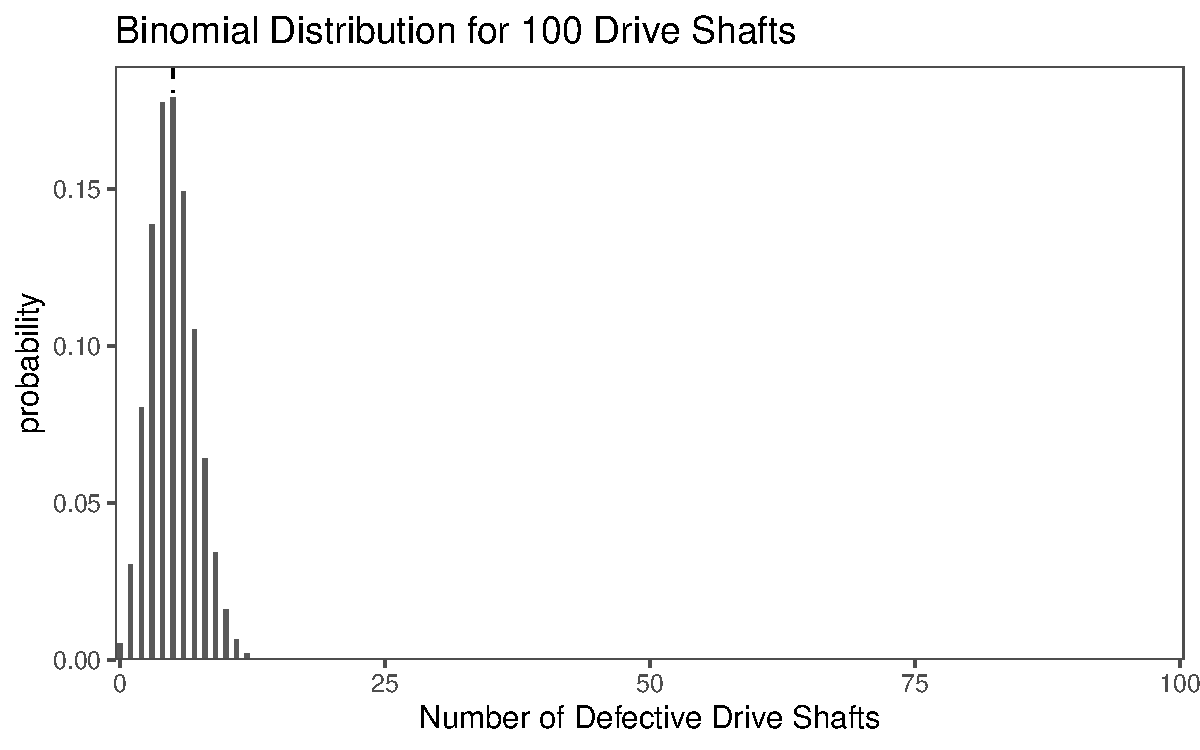
\includegraphics[width=0.95\linewidth,height=\textheight,keepaspectratio]{chapter001_Distributions_files/figure-pdf/fig-bn-ds-1.pdf}

}

\caption{\label{fig-bn-ds}The binomial disitribution and the drive shaft
exercise.}

\end{figure}%

\section{The Normal Distribution}\label{the-normal-distribution}

\begin{figure}[ht]

\centering{

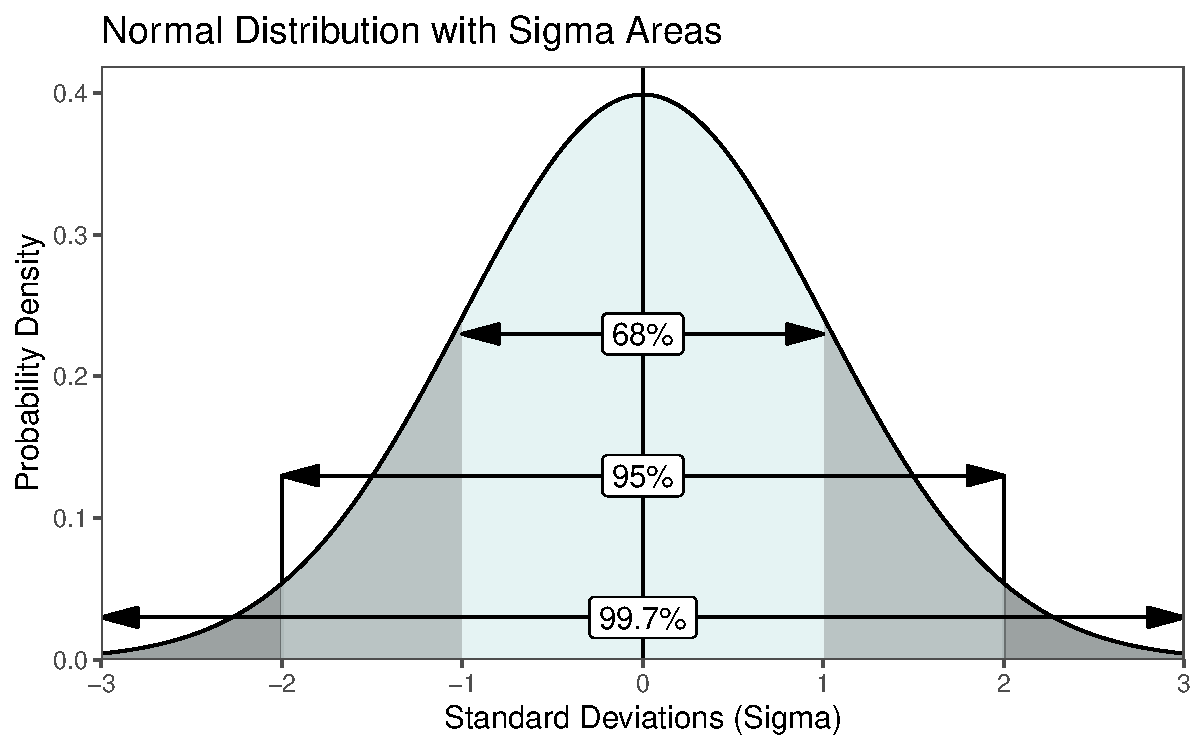
\includegraphics[width=0.75\linewidth,height=\textheight,keepaspectratio]{chapter001_Distributions_files/figure-pdf/fig-normal-dist-1.pdf}

}

\caption{\label{fig-normal-dist}The standarized normal distribution}

\end{figure}%

The normal distribution is a fundamental statistical concept that holds
immense significance in the realms of engineering and production. It is
often referred to as the Gaussian distribution or the bell curve, is a
mathematical model that describes the distribution of data in various
natural and human-made phenomena, see Johnson (1994). It forms a
symmetrical curve when plotted, is centered around a mean
(\hyperref[truemean-gloss]{\(\mu_0\)}) and balanced on both sides
(Figure~\ref{fig-normal-dist}). The spread or dispersion of the data
points is characterized by
\hyperref[truevariance-gloss]{\(\sigma_0^2\)}. Those two parameters
completely define the normal distribution. A remarkable property of the
normal distribution is the empirical rule, which states that
approximately \(68\%\) of the data falls within one standard deviation
from the mean, \(95\%\) falls within two standard deviations, and
\(99.7\%\) falls within three standard deviations
(Figure~\ref{fig-normal-dist}). The existence of the normal distribution
in the real world is a result of the combination of several factors,
including the principles of statistics and probability, the
\hyperref[acronyms_CLT]{CLT}, and the behavior of random processes in
nature and society.

\subsection{Emergence}\label{emergence}

\pandocbounded{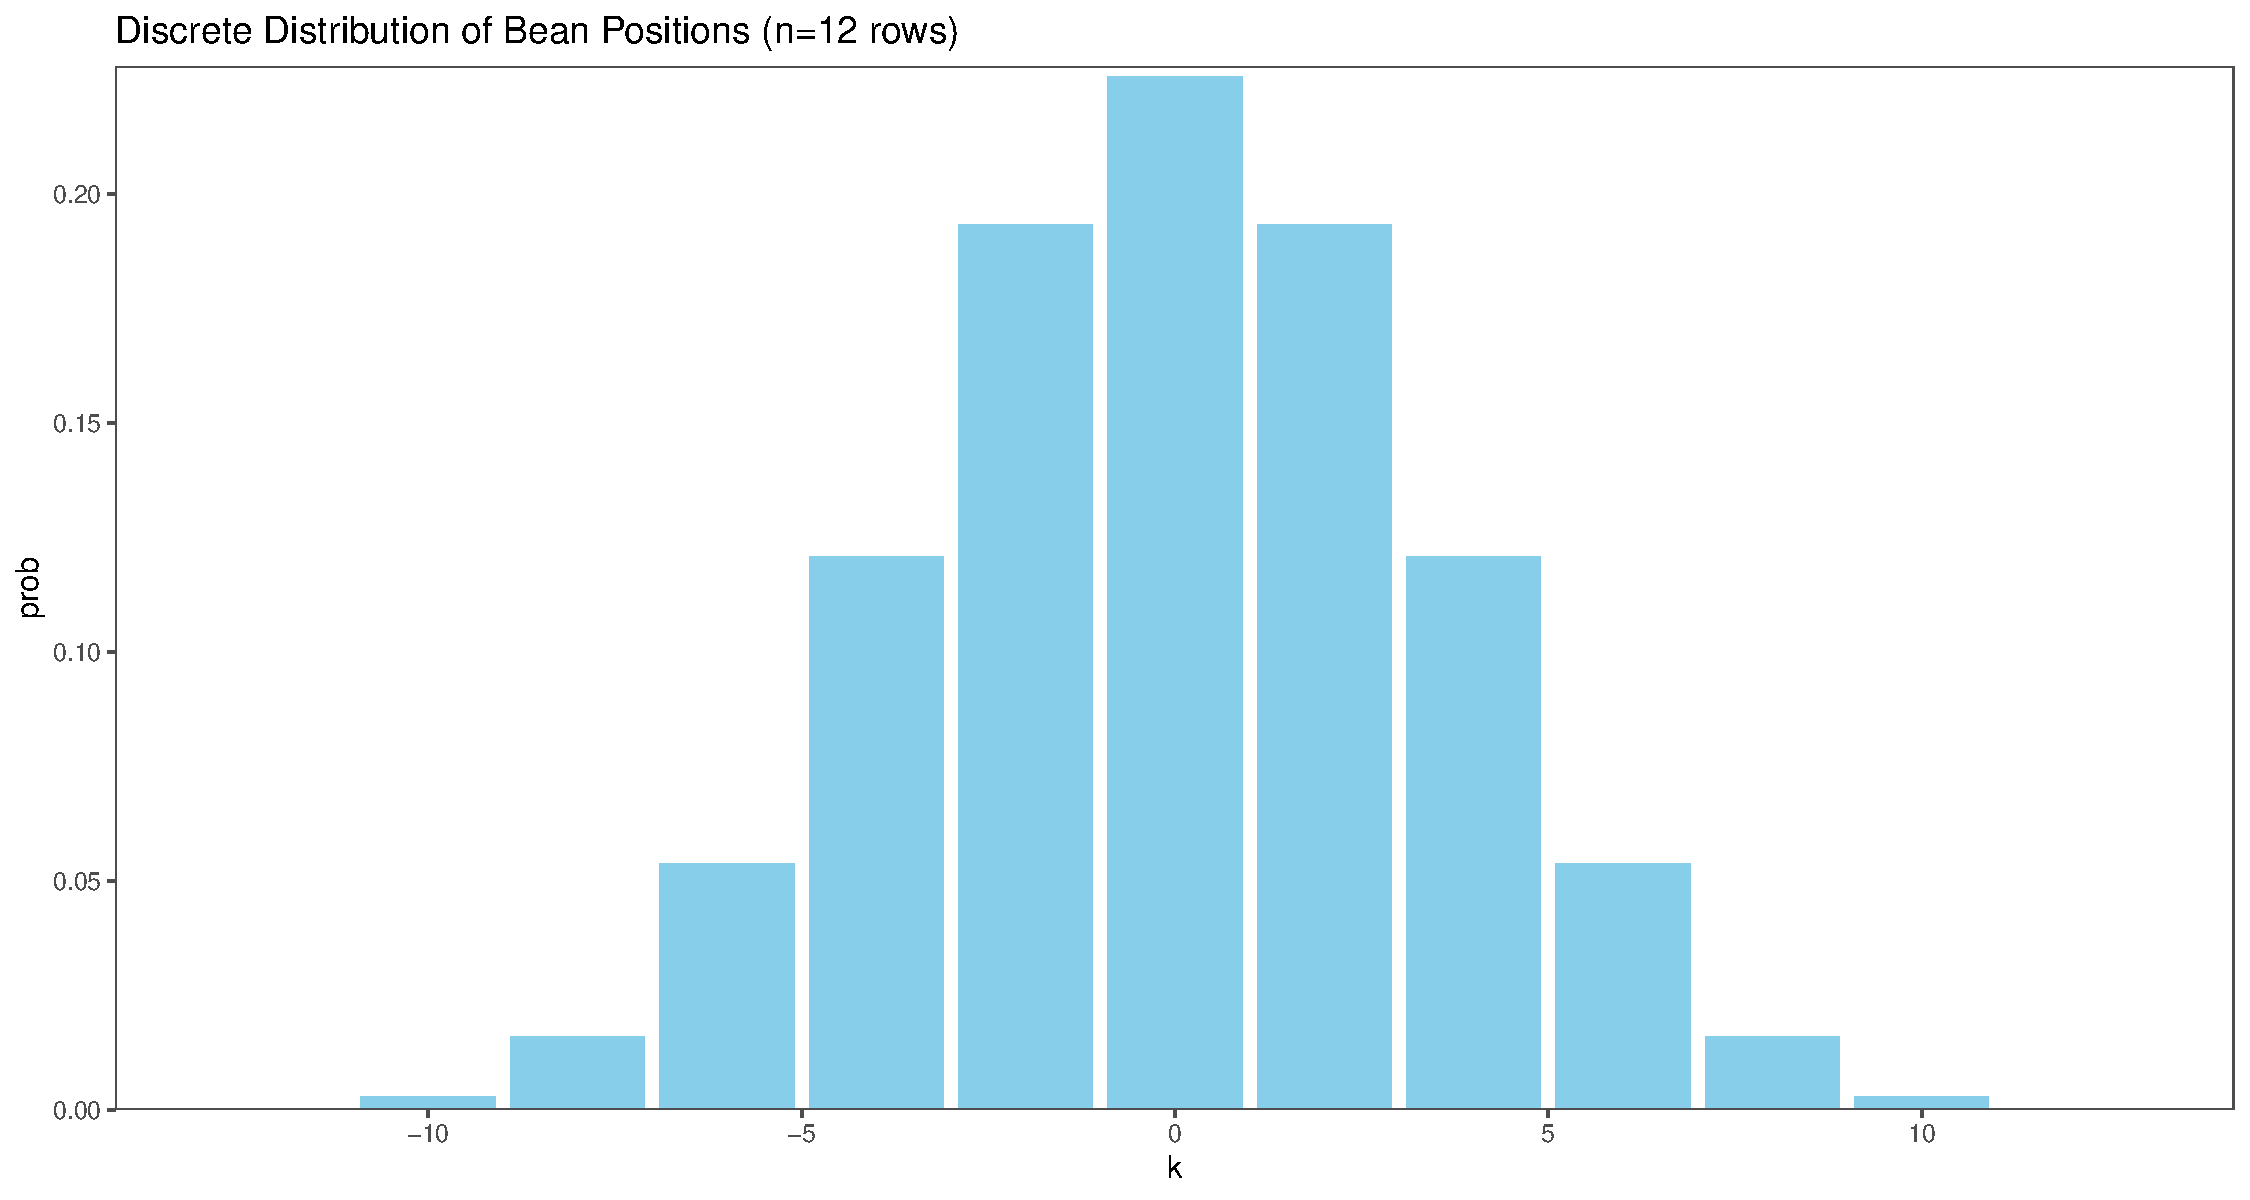
\includegraphics[keepaspectratio]{chapter001_Distributions_files/figure-pdf/unnamed-chunk-1-1.pdf}}

\pandocbounded{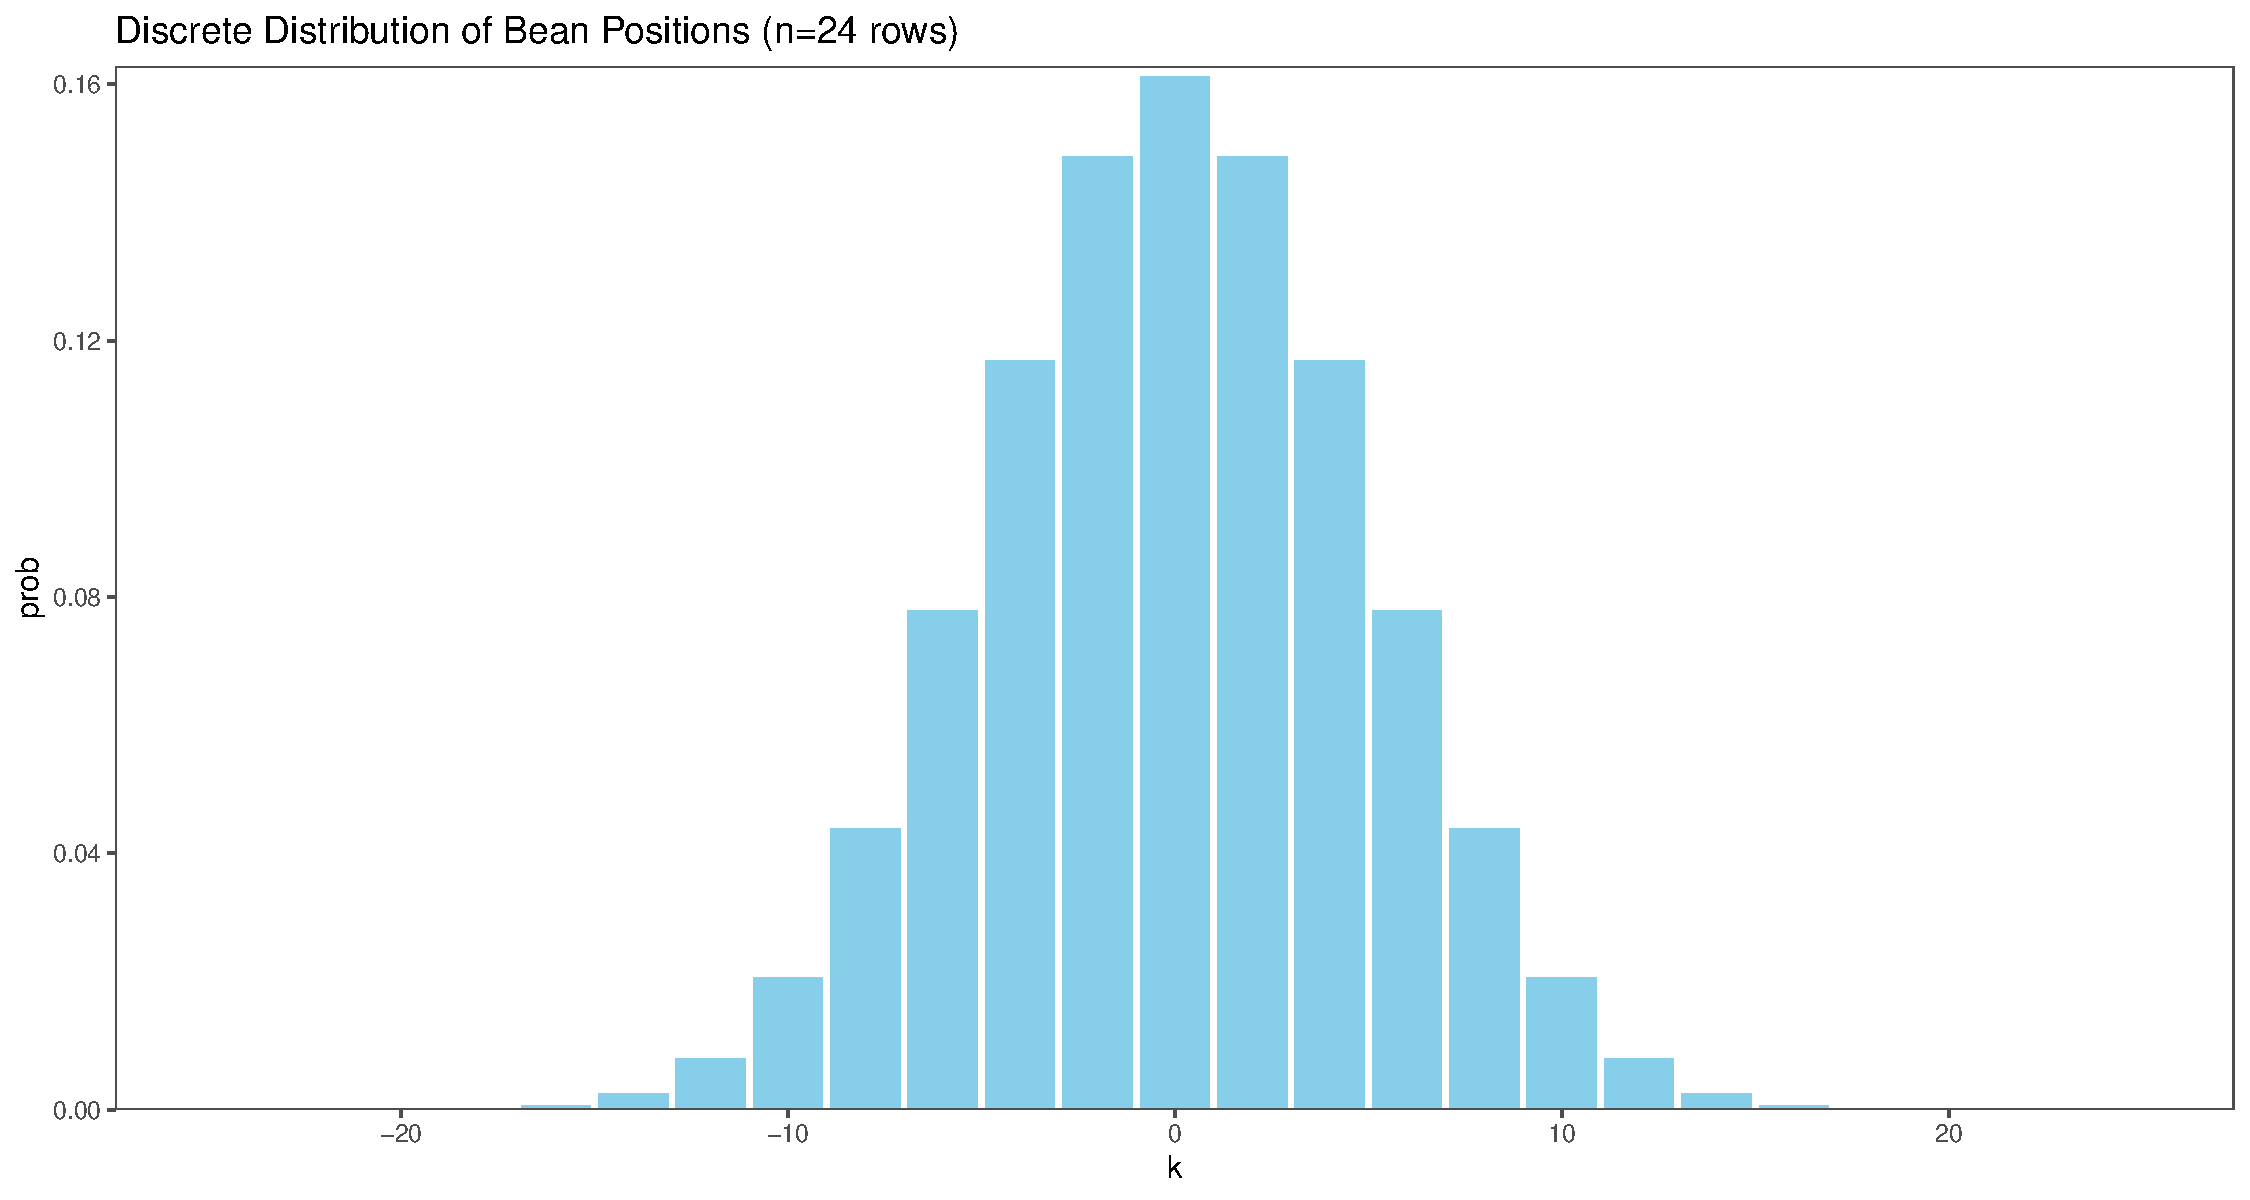
\includegraphics[keepaspectratio]{chapter001_Distributions_files/figure-pdf/unnamed-chunk-2-1.pdf}}

\subsubsection{The math behind}\label{the-math-behind}

\begin{itemize}
\tightlist
\item
  After \(n\) rows a balls final position is the sum of \(n\)
  independent steps: \(S = x_1 + x_2 + \ldots + x_n\) where
  \(x_i = +1 \text{( right) or}  -1 \text{(left)}\)
\item
  \(\text{Number of paths to } k = \binom{n}{(n + k)/2}\)
\end{itemize}

\begin{figure}[ht]

\centering{

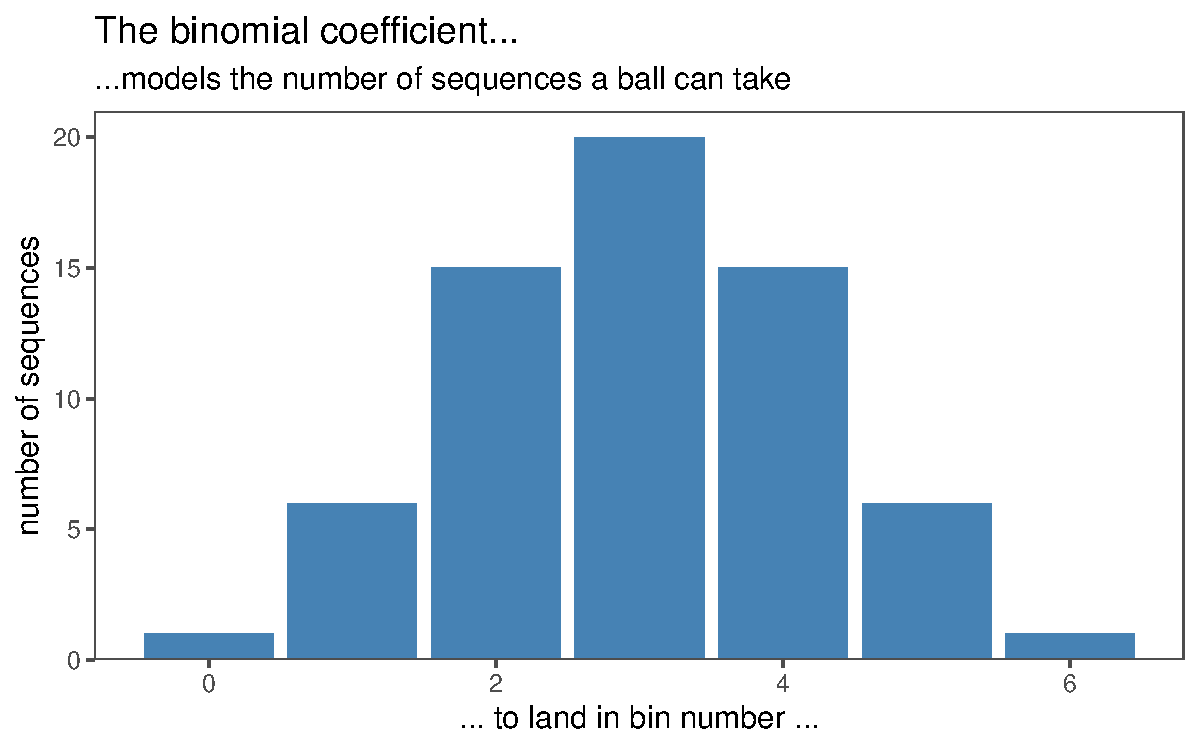
\includegraphics[width=0.75\linewidth,height=\textheight,keepaspectratio]{chapter001_Distributions_files/figure-pdf/fig-galtonboard-dist-1.pdf}

}

\caption{\label{fig-galtonboard-dist}The number of ways a ball can take}

\end{figure}%

\subsubsection{Approximation with a smooth
curve}\label{approximation-with-a-smooth-curve}

\begin{itemize}
\tightlist
\item
  For large \(n\), the binomial distribution looks like a bell curve. It
  can be approximated using the
  \href{https://planetmath.org/StirlingsApproximation}{Stirling
  approximation}
\end{itemize}

\begin{figure}[ht]

\centering{

\pandocbounded{\includegraphics[keepaspectratio]{chapter001_Distributions_files/figure-pdf/fig-normdist-spprox-1.pdf}}

}

\caption{\label{fig-normdist-spprox}The normal distribution can be
approximated using a continous curve}

\end{figure}%

\subsubsection{Binomial Probability}\label{binomial-probability}

\begin{itemize}
\item
  Probability of ending at position \(k\):
  \(P(S=k)\binom{n}{(n + k)/2}(\frac{1}{2})^n\)
\item
  For large \(n\) we can approximate the binomial coefficient:
  \(\binom{n}{m} \approx \frac{n^n}{m^m(n-m)^{n-m}}\sqrt{\frac{n}{2\pi m (n-m)}}\)
  where \(m = (n+k)/2\)
\end{itemize}

\subsubsection{\texorpdfstring{Large \(n\)}{Large n}}\label{large-n}

\begin{itemize}
\tightlist
\item
  Let \(k = x\) (treat as continuous) and \(n\) be large
\item
  After simplification the \hyperref[acronyms_PMF]{PMF} becomes:
  \(P(S=x) \approx \frac{1}{\sqrt{2\pi n}}e^{\frac{-x^2}{2n}}\)
\item
  Replace \(n\) with \(\sigma^2\) and allow for mean \(\mu\):
  \(f(x) = \frac{1}{\sqrt{2\pi\sigma^2}}e^{-\frac{(x-\mu)^2}{2\sigma^2}}\)
\end{itemize}

\subsubsection{The Normal PDF Equation}\label{the-normal-pdf-equation}

\begin{enumerate}
\def\labelenumi{\arabic{enumi}.}
\tightlist
\item
  \(\frac{1}{\sqrt{2\pi\sigma^2}}\): Scaling factor to ensure Total
  Probability = 1
\item
  \(e^{-\frac{(x-\mu)^2}{2\sigma^2}}\): The ``bell'' shape - exponential
  decay based on the distance to the mean
\end{enumerate}

\begin{itemize}
\tightlist
\item
  \textbf{Symmetry}: The term \((x-\mu)^2\) ensures the curve is
  symmetric around \(\mu\)
\item
  \textbf{Peak at mean}: The exponent is zero when \(x = \mu\), giving
  the maximum value
\item
  \textbf{Thickness of Tails}: \(\sigma\) controls how spread out the
  curve is
\end{itemize}

\subsubsection{Parameter influence}\label{parameter-influence}

\begin{figure}[ht]

\centering{

\pandocbounded{\includegraphics[keepaspectratio]{chapter001_Distributions_files/figure-pdf/fig-norm-params-inf-1.pdf}}

}

\caption{\label{fig-norm-params-inf}The influence of distributional
parameters}

\end{figure}%

\subsection{The Buffon needle problem}\label{the-buffon-needle-problem}

\(P\) for crossing a line?

\begin{figure}[ht]

\centering{

\includegraphics[width=0.95\linewidth,height=\textheight,keepaspectratio]{chapter001/buffon.png}

}

\caption{\label{fig-buffon-needle-experiment}An Illustration of the
Buffon Needle Problem.}

\end{figure}%

\subsubsection{Sample Size}\label{sample-size}

\begin{figure}[ht]

\centering{

\pandocbounded{\includegraphics[keepaspectratio]{chapter001_Distributions_files/figure-pdf/fig-buffon-needle-1.pdf}}

}

\caption{\label{fig-buffon-needle}Counting needles leads to an esimtate
of \(\pi\).}

\end{figure}%

\subsubsection{Connection to the Normal
distribution}\label{connection-to-the-normal-distribution}

Why?

Gaussian integral

\subsubsection{\texorpdfstring{\(\pi\) in the Normal
Distribution}{\textbackslash pi in the Normal Distribution}}\label{pi-in-the-normal-distribution}

\begin{align}
I = \int_{-\infty}^{\infty}e^{-kx^2}\,dx\\
I^2 = \int_{-\infty}^{\infty}\int_{-\infty}^{\infty}e^{-k(x^2+y^2)}\,dx\,dy =  \int_{0}^{2\pi}\int_{0}^{\infty}e^{-k^2}r\,dr\,d\theta = \frac{\pi}{k}
\end{align}

\begin{itemize}
\tightlist
\item
  \(e^{-k(x^2+y^2)}=e^{-kr^2}\) is \textbf{radially symmetric}, which
  simplifies the integral
\item
  \(\int_0^{2\pi}\,d\theta = 2\pi\) introduces \(\pi\) in the
  normalization constant of the normal distribution
\end{itemize}

\subsubsection{\texorpdfstring{\(\pi\) in the Buffon Needle
Problem}{\textbackslash pi in the Buffon Needle Problem}}\label{pi-in-the-buffon-needle-problem}

\begin{itemize}
\item
  A needle of length \(L\) is dropped onto a plane with parallel lines
  spaced \(D \geq L\) apart
\item
  Probability \(P\) that the needle crosses a line is
  \(\pi\approx \frac{2l}{D}\frac{\text{Hits}}{N\text{ total number}}\)
\item
  The needles orientation \(\theta\) is uniformly distributed in
  \([0,\pi/2]\)
\item
  The crossing condition depends on \(\sin{\theta}\), and integrating
  over \(\theta\) introduces \(\pi\) through the \emph{average value of
  \(\theta\)} over its domain
\end{itemize}

\subsubsection{What they share}\label{what-they-share}

Both problems translate a probabilistic question into a geometric one,
where \(\pi\) emerges naturally from integrating over angles or
symmetric regions.

\section{Z - Standardization}\label{z---standardization}

\begin{figure}[ht]

\centering{

\includegraphics[width=0.95\linewidth,height=\textheight,keepaspectratio]{chapter001_Distributions_files/figure-pdf/fig-z-scores-raw-1.pdf}

}

\caption{\label{fig-z-scores-raw}How can we compare this data?}

\end{figure}%

The \hyperref[acronyms_Z]{Standard Score / Z-Score (Z)}-standardization,
also known as \hyperref[acronyms_Z]{Z} or \hyperref[acronyms_Z]{Z}, is a
common statistical technique used to transform data into a standard
normal distribution with a mean of \(0\) and a standard deviation of
\(1\) (Taboga 2017). This transformation is useful for comparing and
analyzing data that have different scales and units \eqref{zscore}.

\begin{align}
Z = \frac{x_i - \bar{x}}{sd} \label{zscore}
\end{align}

How the \hyperref[acronyms_Z]{Z} can be applied is shown in
Figure~\ref{fig-z-scores-raw} and Figure~\ref{fig-z-scores-scaled}. The
data for group \texttt{X} and group \texttt{Y} may be measured in
different units ( Figure~\ref{fig-z-scores-raw}). To answer the
question, which of the values \(x_i (i=1\ldots5)\) is more probable, the
single data points are transformed to the respective z-score using
\eqref{zscore}. In Figure~\ref{fig-z-scores-scaled}, the
\hyperref[acronyms_Z]{Z} for both groups are plotted against each other.
The perfect correlation of the datapoints shows, that for every \(x_i\)
the same probability applies. Thus, the datapoints are comparable.

\subsection{Properties of of Z-scores}\label{properties-of-of-z-scores}

\begin{enumerate}
\def\labelenumi{\arabic{enumi}.}
\tightlist
\item
  Shape: The distribution's shape remains normal
\item
  Relative Positions: Values maintain their percentiles
\item
  Outliers: Extreme values \(|z|>3\) are easily flagged
\end{enumerate}

\subsection{Comparison of standardized
data}\label{comparison-of-standardized-data}

\begin{figure}[ht]

\centering{

\includegraphics[width=0.75\linewidth,height=\textheight,keepaspectratio]{chapter001_Distributions_files/figure-pdf/fig-z-scores-scaled-1.pdf}

}

\caption{\label{fig-z-scores-scaled}Normalized data is easier to
compare}

\end{figure}%

\subsection{The Universal Yardstick}\label{the-universal-yardstick}

The standard normal distribution (\(N(0,1)\)) is the reference
distribution (the perfect model).

\begin{itemize}
\tightlist
\item
  \(\bar{x} = 0,\; sd = 1\)
\item
  Empirical Rule (68-65-99.7)

  \begin{itemize}
  \tightlist
  \item
    \(68\%\) of data within \(\pm1sd\)
  \item
    \(95\%\) of data within \(\pm2sd\)
  \item
    \(99.7\%\) of data within \(\pm3sd\)
  \end{itemize}
\end{itemize}

\subsection{The drive shaft exercise -
Z-Standardization}\label{the-drive-shaft-exercise---z-standardization}

\begin{figure}[H]

\centering{

\includegraphics[width=0.95\linewidth,height=\textheight,keepaspectratio]{chapter001_Distributions_files/figure-pdf/fig-ds-z-1.pdf}

}

\caption{\label{fig-ds-z}The standardized data of the drive shaft data.}

\end{figure}%

In Figure~\ref{fig-ds-z} the standardized drive shaft data is shown. The
mean of the data (\(\bar{x}\)) is now centered at \(0\) and the standard
deviation is \(1\). For this case, the specification limits have also
been transferred to the respective \hyperref[acronyms_Z]{Z}-score (even
though they can not be interpreted as such anymore). For every \(x_i\)
the probability to be within a normal distribution is now known. When
comparing this to the transferred specification limits, it is clear to
see that for \texttt{group01} ``most'' of the data points are within the
limits in contrast to \texttt{group03} where none of the data points
lies within the specification limits. When looking at \texttt{group03}
we see, that the \emph{nominal} specification limit is -9.78 standard
deviations away from the centered mean of the datapoints. The
probability of a data point being located there is
\ensuremath{6.8605273\times 10^{-23}} which does not sound an awful lot.
We will dwelve more into such investigation in another chapter, but this
is a first step in the direction of inferential statistics.

\subsection{When Z-Scores Go Wrong}\label{when-z-scores-go-wrong}

\begin{enumerate}
\def\labelenumi{\arabic{enumi}.}
\tightlist
\item
  Non-Normal Data:
\end{enumerate}

\begin{itemize}
\tightlist
\item
  Z-Scores assume normality
\end{itemize}

\begin{enumerate}
\def\labelenumi{\arabic{enumi}.}
\setcounter{enumi}{1}
\tightlist
\item
  Population vs.~Sample
\end{enumerate}

\begin{itemize}
\tightlist
\item
  Use population parameters (\(\mu,\sigma\)) if known, otherwise use
  sample estimates (\(\bar{x},sd\))
\end{itemize}

\begin{enumerate}
\def\labelenumi{\arabic{enumi}.}
\setcounter{enumi}{2}
\tightlist
\item
  Outliers:
\end{enumerate}

\begin{itemize}
\tightlist
\item
  Z-scores are sensitive to outliers
\end{itemize}

\subsection{The Z-transform and the Galton
Board}\label{the-z-transform-and-the-galton-board}

\pandocbounded{\includegraphics[keepaspectratio]{chapter001_Distributions_files/figure-pdf/unnamed-chunk-4-1.pdf}}

\subsubsection{Applying the Z-transform}\label{applying-the-z-transform}

\[Z = \frac{X-\mu}{\sigma}\]

\[Z = \frac{X-\frac{n}{2}}{\frac{\sqrt{n}}{2}}\]

\[\lim_{n\to\infty} P(a\leq Z \leq b)= \int_a^b \frac{1}{\sqrt{2\pi}}e^\frac{-z^2}{2} \,dz \]

\subsubsection{Converting the bionmial Formula to a Normal
Form}\label{converting-the-bionmial-formula-to-a-normal-form}

Stirling appoximation:
\(n!\approx\sqrt{2\pi n} \left( \frac{n}{e} \right)^n\)

Appprox:
\(\binom{n}{k} \approx \frac{\sqrt{2\pi n} \left( \frac{n}{e} \right)^n}{\sqrt{2\pi n} \left( \frac{k}{e} \right)^k \cdot \sqrt{2\pi(n-k)} \left( \frac{n-k}{e} \right)^{n-k}}\)

simplifies to:
\(\binom{n}{k} = \frac{1}{\sqrt{2\pi n p (1-p)}}e^{-\frac{(k-np)^2}{2np(1-p)}}\)

substituting \(p=0.5\):
\(P(X = k) \approx \frac{1}{\sigma\sqrt{2\pi}}e^{-\frac{(k-\mu)^2}{2\sigma^2}}\)

Which is the \hyperref[acronyms_PDF]{PDF}

\subsection{The drive shaft exercise - Normal
Distribution}\label{the-drive-shaft-exercise---normal-distribution}

\begin{figure}[ht]

\centering{

\includegraphics[width=0.75\linewidth,height=\textheight,keepaspectratio]{chapter001_Distributions_files/figure-pdf/fig-ds-nd-1.pdf}

}

\caption{\label{fig-ds-nd}The drive shaft data with the respective
normal distributions.}

\end{figure}%

In Figure~\ref{fig-ds-nd} the \texttt{drive\ shaft\ data} is shown for
each group in a histogram. As an overlay, the respective \emph{normal
distribution} (with the groups \(\bar{x},sd\)) is overlayed. If the data
is normally distributed, is a different question.

\section{\texorpdfstring{\hyperref[acronyms_PDF]{PDF}}{PDF}}\label{section-3}

\begin{figure}[ht]

\centering{

\includegraphics[width=0.75\linewidth,height=\textheight,keepaspectratio]{chapter001/PDF_000.png}

}

\caption{\label{fig-pdf-000-scr}A visual represenstation of the PDF for
the normal distribution.}

\end{figure}%

\begin{align}
f(x) = \frac{1}{\sigma\sqrt{2\pi}}e^{-\frac{1}{2}(\frac{x-\mu}{\sigma})^2}
\end{align}

A \hyperref[acronyms_PDF]{PDF} is a mathematical function that describes
the \emph{likelihood} of a continuous random variable taking on a
particular value. Unlike discrete probability distributions, which
assign probabilities to specific values of a discrete random variable, a
\hyperref[acronyms_PDF]{PDF} describes the relative likelihood of the
variable falling within a particular range of values. The total area
under the curve of a \hyperref[acronyms_PDF]{PDF} over its entire range
is equal to 1, indicating that the variable must take on some value
within that range. In other words, the integral of the
\hyperref[acronyms_PDF]{PDF} over its entire domain equals 1. The
probability of a continuous random variable falling within a specific
interval is given by the integral of the \hyperref[acronyms_PDF]{PDF}
over that interval.

\section{\texorpdfstring{\hyperref[acronyms_CDF]{Cumulative Density
Function (CDF)}}{Cumulative Density Function (CDF)}}\label{section-4}

\begin{figure}[ht]

\centering{

\includegraphics[width=0.75\linewidth,height=\textheight,keepaspectratio]{chapter001/CDF_000.png}

}

\caption{\label{fig-cdf-000-scr}A visual represenstation of the CDF for
the normal distribution.}

\end{figure}%

A \hyperref[CDF]{cumulative density function (CDF)}, also known as a
cumulative distribution function, describes the probability that a
random variable will take on a value less than or equal to a given
point. It is the integral of the \hyperref[acronyms_PDF]{PDF} from
negative infinity to a certain value. The \hyperref[acronyms_CDF]{CDF}
provides a comprehensive view of the probability distribution of a
random variable by showing how the probability accumulates as the value
of the random variable increases. Unlike the
\hyperref[acronyms_PDF]{PDF}, which gives the probability density at a
particular point, the CDF gives the cumulative probability up to that
point.

\begin{align}
z &= \frac{x-\mu}{\sigma} \nonumber \\
\varphi(x) &= \frac{1}{2\pi}e^{\frac{-z^2}{2}} \\
\phi(x)& = \int \frac{1}{2\pi}e^{\frac{-x^2}{2}} \, dx \\
\lim_{x\to\infty} \phi(x) &= 1 \nonumber \\
\lim_{x\to - \infty} \phi(x) &= 0 \nonumber
\end{align}

\section{Likelihood and Probability}\label{likelihood-and-probability}

\begin{figure}[ht]

\centering{

\includegraphics[width=0.75\linewidth,height=\textheight,keepaspectratio]{chapter001/likelihood_prob.png}

}

\caption{\label{fig-lp}The subtle difference between likelihood and
probability.}

\end{figure}%

\begin{description}
\tightlist
\item[Likelihood]
refers to the chance or plausibility of a particular event occurring
given certain evidence or assumptions. It is often used in statistical
inference, where it indicates how well a particular set of parameters
(or hypotheses) explain the observed data. Likelihood is a measure of
how compatible the observed data are with a specific hypothesis or
model.
\item[Probability]
represents the measure of the likelihood that an event will occur. It is
a quantification of uncertainty and ranges from \(0\) (indicating
impossibility) to \(1\) (indicating certainty). Probability is commonly
used to assess the chances of different outcomes in various scenarios.
\end{description}

In summary, while both likelihood and probability deal with the chance
of events occurring, likelihood is often used in the context of
comparing different \emph{hypotheses or models} based on \emph{observed
data}, while probability is more broadly used to quantify the chances of
\emph{events happening} in \emph{general}.

\subsection{Exercise}\label{exercise-1}

\begin{longtable}[]{@{}llllll@{}}
\caption{Exercise Data}\tabularnewline
\toprule\noalign{}
Machine & Sample 1 & Sample 2 & Sample 3 & Sample 4 & Sample 5 \\
\midrule\noalign{}
\endfirsthead
\toprule\noalign{}
Machine & Sample 1 & Sample 2 & Sample 3 & Sample 4 & Sample 5 \\
\midrule\noalign{}
\endhead
\bottomrule\noalign{}
\endlastfoot
\textbf{Machine X} & 44 & 46 & 45 & 47 & 43 \\
\textbf{Machine Y} & 52 & 50 & 53 & 49 & 51 \\
\textbf{Machine Z} & 40 & 42 & 39 & 41 & 43 \\
\end{longtable}

\begin{table}

\caption{\label{tbl-exercise-z}Exercise Data}

\centering{

\fontsize{12.0pt}{14.0pt}\selectfont
\begin{tabular*}{\linewidth}{@{\extracolsep{\fill}}rrr}
\toprule
machine\_x & machine\_y & machine\_z \\ 
\midrule\addlinespace[2.5pt]
44 & 52 & 40 \\ 
46 & 50 & 42 \\ 
45 & 53 & 39 \\ 
47 & 49 & 41 \\ 
43 & 51 & 43 \\ 
\bottomrule
\end{tabular*}

}

\end{table}%

\begin{enumerate}
\def\labelenumi{\arabic{enumi}.}
\tightlist
\item
  calculate \(\bar{x}\) and \(sd\)
\item
  Compute z-scores
\item
  Flag anomalies
\item
  Recommend actions
\end{enumerate}

\begin{center}\rule{0.5\linewidth}{0.5pt}\end{center}

\begin{table}

\caption{\label{tbl-exercise-z-res}Results}

\centering{

\fontsize{12.0pt}{14.0pt}\selectfont
\begin{tabular*}{\linewidth}{@{\extracolsep{\fill}}lrrr}
\toprule
machine & mean\_cycle\_time & sd\_cycle\_time & var\_cycle\_time \\ 
\midrule\addlinespace[2.5pt]
machine\_x & 45 & 1.581139 & 2.5 \\ 
machine\_y & 51 & 1.581139 & 2.5 \\ 
machine\_z & 41 & 1.581139 & 2.5 \\ 
\bottomrule
\end{tabular*}

}

\end{table}%

\begin{center}\rule{0.5\linewidth}{0.5pt}\end{center}

\begin{table}

\caption{\label{tbl-exercise-z-scores}Results for z score}

\centering{

\fontsize{12.0pt}{14.0pt}\selectfont
\begin{tabular*}{\linewidth}{@{\extracolsep{\fill}}rc}
\toprule
cycle\_time\_s & scaled\_data \\ 
\midrule\addlinespace[2.5pt]
\multicolumn{2}{l}{machine\_x} \\[2.5pt] 
\midrule\addlinespace[2.5pt]
44 & -0.6324555 \\ 
46 & 0.6324555 \\ 
45 & 0.0000000 \\ 
47 & 1.2649111 \\ 
43 & -1.2649111 \\ 
\midrule\addlinespace[2.5pt]
\multicolumn{2}{l}{machine\_y} \\[2.5pt] 
\midrule\addlinespace[2.5pt]
52 & 0.6324555 \\ 
50 & -0.6324555 \\ 
53 & 1.2649111 \\ 
49 & -1.2649111 \\ 
51 & 0.0000000 \\ 
\midrule\addlinespace[2.5pt]
\multicolumn{2}{l}{machine\_z} \\[2.5pt] 
\midrule\addlinespace[2.5pt]
40 & -0.6324555 \\ 
42 & 0.6324555 \\ 
39 & -1.2649111 \\ 
41 & 0.0000000 \\ 
43 & 1.2649111 \\ 
\bottomrule
\end{tabular*}

}

\end{table}%

\section{\texorpdfstring{Chi\textsuperscript{2} -
Distribution}{Chi2 - Distribution}}\label{chi2---distribution}

\begin{figure}[H]

\begin{minipage}{0.45\linewidth}

\centering{

\pandocbounded{\includegraphics[keepaspectratio]{chapter001_Distributions_files/figure-pdf/fig-chi-2-1.pdf}}

}

\subcaption{\label{fig-chi-2-1}a normal distribution}

\end{minipage}%
%
\begin{minipage}{0.10\linewidth}
~\end{minipage}%
%
\begin{minipage}{0.45\linewidth}

\centering{

\pandocbounded{\includegraphics[keepaspectratio]{chapter001_Distributions_files/figure-pdf/fig-chi-2-2.pdf}}

}

\subcaption{\label{fig-chi-2-2}the standard normal variable square
(\(dof = 1\))}

\end{minipage}%
\newline
\begin{minipage}{\linewidth}

\centering{

\pandocbounded{\includegraphics[keepaspectratio]{chapter001_Distributions_files/figure-pdf/fig-chi-2-3.pdf}}

}

\subcaption{\label{fig-chi-2-3}the \(\chi^2\) distributions with varying
degrees of freedom}

\end{minipage}%

\caption{\label{fig-chi-2}What a \(\chi^2\) distribution reprepresents
and how it relates to a the normal distribution.}

\end{figure}%

The \(\chi^2\) distribution is a continuous probability distribution
that is widely used in statistics (Taboga 2017). It is often used to
test hypotheses about the independence of categorical variables.

\begin{align}
\chi^2 = \sum_{k = 1}^n \frac{(O_k - E_k)^2}{E_k}
\end{align}

The connection between the chi-squared distribution and sample variance
holds significant importance in statistics.

\begin{enumerate}
\def\labelenumi{\arabic{enumi}.}
\item
  \textbf{Distribution of Sample Variance:} When calculating the sample
  variance from a dataset, it follows a chi-squared distribution.
  Specifically, for a random sample from a normally distributed
  population with mean \hyperref[truemean-gloss]{\(\mu_0\)} and variance
  \hyperref[truevariance-gloss]{\(\sigma_0^2\)}, the sample variance
  (adjusted for bias) divided by
  \hyperref[truevariance-gloss]{\(\sigma_0^2\)} follows a \(\chi^2\)
  distribution with \(n-1\) \hyperref[acronyms_dof]{dof}, where \(n\) is
  the sample size.
\item
  \textbf{Hypothesis Testing:} In statistical analysis, hypothesis
  testing is a common technique for making inferences about populations
  using sample data. The \(\chi^2\) distribution plays a crucial role in
  hypothesis testing, especially when comparing variances between
  samples.

  \begin{itemize}
  \tightlist
  \item
    \textbf{\(\chi^2\) Test for Variance:} The \(\chi^2\) distribution
    is used to test whether the variance of a sample matches a
    hypothesized variance. This is applicable in various scenarios, such
    as quality control, to assess the consistency of a manufacturing
    process.
  \end{itemize}
\item
  \textbf{Confidence Intervals:} When estimating population parameters
  like population variance, it's essential to establish confidence
  intervals. The \(\chi^2\) distribution aids in constructing these
  intervals, allowing researchers to quantify the uncertainty associated
  with their parameter estimates.
\item
  \textbf{Model Assessment:} In regression analysis, the \(\chi^2\)
  distribution is related to the F-statistic, which assesses the overall
  significance of a regression model. It helps determine whether the
  regression model is a good fit for the data.
\end{enumerate}

In summary, the link between the chi-squared distribution and sample
variance is fundamental in statistical analysis. It empowers
statisticians and analysts to make informed decisions about population
parameters based on sample data and evaluate the validity of statistical
models. Understanding this relationship is essential for those working
with data and conducting statistical investigations.

\subsection{\texorpdfstring{The drive shaft exercise -
Chi\textsuperscript{2}
Distribution}{The drive shaft exercise - Chi2 Distribution}}\label{the-drive-shaft-exercise---chi2-distribution}

\begin{figure}[ht]

\centering{

\includegraphics[width=0.95\linewidth,height=\textheight,keepaspectratio]{chapter001_Distributions_files/figure-pdf/fig-ds-chi-1.pdf}

}

\caption{\label{fig-ds-chi}The \(\chi^2\) disitribution of the drive
shaft data.}

\end{figure}%

In Figure~\ref{fig-ds-chi} the squared standad deviation for every
datapoint (from the stanardized data) is shown as a histogram for every
group with an overlayed (and scaled) density plot. In the background of
every group the theoretical \(\chi^2\)-distribution with \(dof = 1\) is
plotted to visually compare the empirical distribution of the datapoints
to the theorectial.

\section{t - Distribution}\label{t---distribution}

\begin{figure}[ht]

\centering{

\includegraphics[width=0.95\linewidth,height=\textheight,keepaspectratio]{chapter001_Distributions_files/figure-pdf/fig-t-dist-1.pdf}

}

\caption{\label{fig-t-dist}PDF of t-distribution with varying \(dof\)}

\end{figure}%

The t-distribution, also known as the Student's t-distribution (Student
1908), is a probability distribution that plays a significant role in
statistics\footnote{William Sealy Gosset (June 13, 1876 - October 16,
  1937) was a pioneering statistician known for developing the
  t-distribution, a key tool in modern statistical analysis.}. It is a
symmetric distribution with a bell-shaped curve, similar to the normal
distribution, but with heavier tails. The key significance of the
t-distribution lies in its application to inferential statistics,
particularly in hypothesis testing and confidence interval estimation.

\begin{enumerate}
\def\labelenumi{\arabic{enumi}.}
\item
  \textbf{Small Sample Sizes:} When dealing with small sample sizes
  (typically less than 30), the t-distribution is used to make
  inferences about population parameters, such as the mean. This is
  crucial because the normal distribution assumptions are often violated
  with small samples.
\item
  \textbf{Accounting for Variability:} The t-distribution accounts for
  the variability inherent in small samples. It provides wider
  confidence intervals and more conservative hypothesis tests compared
  to the normal distribution, making it more suitable for situations
  where sample size is limited.
\item
  \textbf{Degrees of Freedom:} The shape of the t-distribution is
  determined by a parameter called \hyperref[acronyms_dof]{dof}. As the
  \hyperref[acronyms_dof]{dof} increases, the t-distribution approaches
  the normal distribution. When df is small, the tails of the
  t-distribution are fatter, allowing for greater uncertainty in
  estimates.
\end{enumerate}

Statisticians found that if they took samples of a constant size from a
normal population, computed a statistic called a \emph{t-score} for each
sample, and put those into a relative frequency distribution, the
distribution would be the same for samples of the same size drawn from
any normal population. The shape of this sampling distribution of t's
varies somewhat as sample size varies, but for any \(n\), it is always
the same. For example, for samples of \(5\), \(90\%\) of the samples
have t-scores between \(-1.943\) and \(+1.943\), while for samples of
\(15\), \(90\%\) have t-scores between \(\pm 1.761\). The bigger the
samples, the narrower the range of scores that covers any particular
proportion of the samples \eqref{tscore} (Note the similarity to
\eqref{zscore}). Since the \emph{t-score} is computed for every \(x_i\)
the resulting sampling distribution is called the
\emph{t-disitribution}.

\begin{align}
t_i = \frac{x_i - \mu_o}{sd/\sqrt{n}} \label{tscore}
\end{align}

In Figure~\ref{fig-t-dist} it is shown, that with increasing
\hyperref[acronyms_dof]{dof} (in this case \emph{sample size}), the
\emph{t-distribution} approximates a normal distribution (gray area).
Figure~\ref{fig-t-dist} also shows an example of the
\emph{t-distribution} in action. Of all possible samples with 9
\hyperref[dof]{\(dof\)} \(0.025\;(2\frac{1}{2}\%)\) of those samples
would have t-scores greater than \(2.262\), and \(.975\;(97.5\%)\) would
have t-scores less than \(2.262\). The advantage of the \emph{t-score}
and \emph{t-distribution} is clearly visible. All these values can be
computed from sampled data, the population can remain \emph{estimated}
\eqref{tscore}.

\subsection{The drive shaft exercise -
t-Distribution}\label{the-drive-shaft-exercise---t-distribution}

The t-score computation and the z-standardization look very familiar.
While the z-score calculation needs some population parameters, the
t-score calculation does not need such. It therefore allows us, to
estimate population parameters based on a sample - a very frequent use
case in statistics.

Suppose we have some data (maybe the drive shaft exercise?) with which
calculations can be done. First, the mean \(\bar{x}\) and \(sd\) is
calculated according to \eqref{mean} and \eqref{sd}. After this, the
\hyperref[acronyms_cl]{confidence level (cl)} (we will get to this later
in more detail) is specified. A value of \(95\%\) is a common choice of
\hyperref[acronyms_cl]{cl}.

\begin{align}
ci &= 0.95 \quad \text{(for a 95\% confidence level)}
\end{align}

Then the \hyperref[acronyms_SE]{Standard Error (SE)} is calculated using
\eqref{se}, which takes the \(sd\) and \(n\) of a sample into account
(notice, how we did not use any population estimation?).

\begin{align}
SE &= \frac{sd}{\sqrt{n}} \label{se}
\end{align}

In the next step, the critical \emph{t-score} is calculated using the
\hyperref[acronyms_cl]{cl} as shown in \eqref{tscore}. \emph{qt} in this
case returns the value of the inverse \hyperref[acronyms_CDF]{CDF} of
the t-distribution given a certain random variable (or datapoint
\(x_i\)) and \(n-1\) \hyperref[acronyms_dof]{dof}. Think of it as an
automated look up in long statistical tables.

\begin{align}
% Step 5: Calculate the T-score
t_{score} &= qt\left(\frac{1 - ci}{2}, df = n - 1\right) \label{tscore}
\end{align}

With this, the \emph{margin of error} can be calculated using the
\hyperref[acronyms_SE]{SE} and the \emph{t-score} as shown in
\eqref{errormargin}.

\begin{align}
% Step 6: Calculate the margin of error
margin\;of\;error &= t_{score} \times SE \label{errormargin}
\end{align}

In the last step the \hyperref[ci]{Confidence Interval} is calculated
for the \texttt{lower} and the \texttt{upper} bound with
\eqref{cilobound} and \eqref{cihibound}.

\begin{align}
% Step 7: Determine the confidence interval
lo &= \bar{x} - margin\;of\;error \label{cilobound} \\
hi &= \bar{x} + margin\;of\;error \label{cihibound}
\end{align}

It all looks and feels very similar to using the normal disitrbution.
Why this is the case, is shown in Figure~\ref{fig-ds-t}. In
\textbf{?@fig-ds-t-1} the raw dataset is shown with the underlayed
specification limits for the manufacturing of the drive shaft. For some
groups the judgement if the drive shaft is wihtin specification is quite
clear (\texttt{group\ 1}, \texttt{group\ 2} and \texttt{group\ 5}). For
the other groups, this can not be done so easily. For the drive shaft
data, we of course now some population data, therefore the \emph{normal
distribution} can be compared to the \emph{t-distribution}. This is done
in \textbf{?@fig-ds-t-2}. On the \texttt{x-axis} the diameter is shown,
the \texttt{y-axis} depicts the groups (as before). The distribution on
top of the estimated parameters is the population (normal distribution),
the distribution on the bottom follow a \emph{t-distribution}. With
\(n>30\) (as for this dataset), the difference between distribution is
very small, further showcasing the use of the \emph{t-distribution}
(also see Figure~\ref{fig-t-dist} for comparison).

\begin{figure}[ht]

\centering{

\includegraphics[width=0.95\linewidth,height=\textheight,keepaspectratio]{chapter001_Distributions_files/figure-pdf/fig-ds-t-1.pdf}

}

\caption{\label{fig-ds-t}The drive shaft data with normal disitribution,
t-distribution and confidence intervalls using the t-distribution}

\end{figure}%

\section{F - Statistics}\label{f---statistics}

\emph{F-statistics}, also known as the \emph{F-test} or \emph{F-ratio},
is a statistical measure used in \hyperref[acronyms_ANOVA]{Analysis of
Variance (ANOVA)} and regression analysis (Taboga 2017). It assesses the
ratio of two variances, indicating the extent to which the variability
between groups or models is greater than the variability within those
groups or models. The \emph{F-statistic} plays a crucial role in
hypothesis testing and model comparison.

Significance of F-statistics: The significance of the F-statistic lies
in its ability to help researchers determine whether the differences
between group means or the goodness-of-fit of a regression model are
statistically significant. In \hyperref[acronyms_ANOVA]{ANOVA}, a high
F-statistic suggests that at least one group mean differs significantly
from the others, while in regression analysis, it indicates whether the
regression model as a whole is a good fit for the data.

Applications of F-statistics: 1. \textbf{Analysis of Variance
\hyperref[acronyms_ANOVA]{ANOVA}:} F-statistics are extensively used in
\hyperref[acronyms_ANOVA]{ANOVA} to compare means across two or more
groups. It helps determine whether there are significant differences
among the means of these groups. For example, an
\hyperref[acronyms_ANOVA]{ANOVA} might be used to compare the mean test
scores of students taught using different teaching methods.

\begin{enumerate}
\def\labelenumi{\arabic{enumi}.}
\setcounter{enumi}{1}
\tightlist
\item
  \textbf{Regression Analysis:} F-statistics are used in regression
  analysis to assess the overall significance of a regression model.
  Specifically, in multiple linear regression, it helps determine
  whether the model, which includes multiple predictor variables, is
  better at explaining the variance in the response variable compared to
  a model with no predictors. It tests the null hypothesis that all
  coefficients of the model are equal to zero.
\end{enumerate}

\begin{figure}[ht]

\centering{

\includegraphics[width=0.95\linewidth,height=\textheight,keepaspectratio]{chapter001_Distributions_files/figure-pdf/fig-f-dist-01-1.pdf}

}

\caption{\label{fig-f-dist-01}F-distribution for \(dof_1\) on the
horizontal and \(dof_2\) on the vertical axis}

\end{figure}%

The \hyperref[acronyms_dof]{dof} in an \emph{F-distribution} refer to
the two sets of numbers that determine the shape and properties of the
distribution (Figure~\ref{fig-f-dist-01}).

Numerator Degrees of Freedom (\(dof_1\)): The numerator degrees of
freedom, often denoted as \(dof_1\), is associated with the variability
between groups or models in statistical analyses
(Figure~\ref{fig-f-dist-01} - horizontal axis). In the context of
\hyperref[acronyms_ANOVA]{ANOVA}, it represents the
\hyperref[acronyms_dof]{dof} associated with the differences among group
means. In regression analysis, it is related to the number of predictors
or coefficients being tested simultaneously.

Denominator Degrees of Freedom (\(dof_2\)): The denominator degrees of
freedom, often denoted as \(dof_2\), is associated with the variability
within groups or models (Figure~\ref{fig-f-dist-02} - vertical axis). In
\hyperref[acronyms_ANOVA]{ANOVA}, it represents the degrees of freedom
associated with the variability within each group. In regression
analysis, it is related to the error or residual degrees of freedom,
indicating the remaining variability not explained by the model.

The F-distribution is used to compare two variances: one from the
numerator and the other from the denominator. The F-statistic,
calculated as the ratio of these variances, follows an F-distribution
\eqref{fdist}.

\begin{align}
f(x; dof_1, dof_2) = \frac{{\Gamma\left(\frac{{dof_1 + dof_2}}{2}\right)}}{{\Gamma\left(\frac{{dof_1}}{2}\right)\Gamma\left(\frac{{dof_2}}{2}\right)}} \left(\frac{{dof_1}}{{dof_2}}\right)^{\frac{{dof_1}}{2}} \frac{{x^{\frac{{dof_1}}{2} - 1}}}{{\left(1 + \frac{{dof_1}}{{dof_2}}x\right)^{\frac{{dof_1 + dof_2}}{2}}}} \label{fdist} \\
F_{m,n} = \frac{\chi^2_m/m}{\chi^2_n/n} 
\end{align}

\begin{figure}

\begin{minipage}{\linewidth}

\begin{figure}[H]

\centering{

\includegraphics[width=0.95\linewidth,height=\textheight,keepaspectratio]{chapter001_Distributions_files/figure-pdf/fig-f-dist-02-1.pdf}

}

\caption{\label{fig-f-dist-02}the maximum density as a function of
\(dof_1\) and \(dof_2\) in a continous parameter space}

\end{figure}%

\end{minipage}%

\end{figure}%

In practical terms: A higher numerator degrees of freedom (\(dof_1\))
suggests that there are more groups or predictors being compared, which
may result in larger F-statistic values. A higher denominator degrees of
freedom (\(dof_2\)) implies that there is more data within each group or
model, which may lead to smaller F-statistic values. The F-distribution
is right-skewed and always positive. It has different shapes depending
on the values of \(dof_1\) and \(dof_2\) (Figure~\ref{fig-f-dist-02}).
The exact shape is determined by these degrees of freedom and cannot be
altered by changing sample sizes or data values
(Figure~\ref{fig-f-dist-02}). Researchers use F-distributions to conduct
hypothesis tests, such as F-tests in ANOVA and F-tests in regression, to
determine if there are significant differences between groups or if a
regression model is statistically significant.

In summary, \hyperref[acronyms_dof]{dof} in the F-distribution are
critical in hypothesis testing and model comparisons. They help quantify
the variability between and within groups or models, allowing
statisticians to assess the significance of observed differences and
make informed statistical decisions.

\section{Interconnections}\label{interconnections}

\begin{enumerate}
\def\labelenumi{\arabic{enumi}.}
\item
  Normal Distribution The \textbf{Normal Distribution} is characterized
  by its mean (\(\mu\)) and standard deviation (\(\sigma\)), see
  Figure~\ref{fig-interconnections}. It serves as the foundation for
  many statistical analyses.
\item
  Standardized Normal Distribution The \textbf{Standardized Normal
  Distribution}, denoted as \(Z \sim N(0, 1)\), is a special case of the
  normal distribution. It has a mean (\(\mu\)) of \(0\) and a standard
  deviation (\(\sigma\)) of \(1\). It is obtained by standardizing a
  normal distribution variable \(X\): \(Z = \frac{X - \mu}{\sigma}\)
  (Figure~\ref{fig-interconnections}).
\item
  t Distribution The \textbf{t Distribution} is related to the normal
  distribution and depends on \hyperref[acronyms_dof]{dof}. As
  \hyperref[acronyms_dof]{dof} increases, the t-distribution approaches
  the standard normal distribution (Figure~\ref{fig-interconnections}).
\item
  Chi-Square Distribution The \textbf{Chi-Square Distribution} is
  indirectly connected to the normal distribution through the concept of
  ``sum of squared standard normals.'' When standard normal random
  variables (\(Z\)) are squared and summed, the resulting distribution
  follows a chi-square distribution.
\item
  F Distribution The \textbf{F Distribution} arises from the ratio of
  two independent chi-square distributed random variables. It is used
  for comparing variances between groups in statistical tests like
  \hyperref[acronyms_ANOVA]{ANOVA}.
\end{enumerate}

\begin{figure}[H]

\centering{

\includegraphics[width=0.75\linewidth,height=\textheight,keepaspectratio]{chapter000/009_DistributionConnection.png}

}

\caption{\label{fig-interconnections}The distributions are
interconnected in several different ways.}

\end{figure}%

\section{Weibull - Distribution}\label{weibull---distribution}

\begin{figure}[ht]

\centering{

\includegraphics[width=0.95\linewidth,height=\textheight,keepaspectratio]{chapter001_Distributions_files/figure-pdf/fig-wbll-dist-1.pdf}

}

\caption{\label{fig-wbll-dist}The weibull distribution and the influence
of \(\beta\) and \(\lambda\)}

\end{figure}%

The Weibull distribution is a probability distribution frequently used
in statistics and reliability engineering to model the time until an
event, particularly failures or lifetimes. It is named after Wallodi
Weibull\footnote{Waloddi Weibull (1887--1979) was a Swedish engineer and
  statistician known for his work on the Weibull distribution, which is
  widely used in reliability engineering and other fields.}, who
developed it in the mid-20th century (Weibull 1951).

The Weibull distribution is characterized by two parameters:

\textbf{Shape Parameter (\(\beta\)):} This parameter determines the
shape of the distribution curve and can take on values greater than 0.
Depending on the value of \(\beta\), the Weibull distribution can
exhibit different behaviors:

If \(\beta < 1\), the distribution has a decreasing failure rate,
indicating that the probability of an event occurring decreases over
time. This is often associated with ``infant mortality'' or early-life
failures. If \(\beta = 1\), the distribution follows an exponential
distribution with a constant failure rate over time. If \(\beta > 1\),
the distribution has an increasing failure rate, suggesting that the
event becomes more likely as time progresses. This is often associated
with ``wear-out'' failures.

\textbf{Scale Parameter (\(\lambda\)):} This parameter represents a
characteristic scale or location on the time axis. It influences the
position of the distribution on the time axis. A larger \(\lambda\)
indicates that events are more likely to occur at later times.

\textbf{Applications:} - Reliability Engineering: The Weibull
distribution is extensively used in reliability engineering to assess
the lifetime and failure characteristics of components and systems.
Engineers can estimate the distribution parameters from data to predict
product reliability, set warranty periods, and plan maintenance
schedules.

\begin{itemize}
\item
  Survival Analysis: In medical research and epidemiology, the Weibull
  distribution is employed to analyze survival data, such as time until
  the occurrence of a disease or death. It helps in modeling and
  understanding the progression of diseases and the effectiveness of
  treatments.
\item
  Economics and Finance: The Weibull distribution is used in finance to
  model the time between financial events, like market crashes or loan
  defaults. It can provide insights into risk assessment and portfolio
  management.
\end{itemize}

\subsection{The drive shaft exercise - Weibull
distribution}\label{the-drive-shaft-exercise---weibull-distribution}

The Weibull distribution can be applied to estimate the probability of a
part to fail after a given time. Suppose there have been \(n=100\) drive
shafts produced. In order to assure that the assembled drive shaft would
last during their service time, they have been tested in a test-stand
that mimics the mission profile\footnote{A mission profile for parts is
  a detailed plan specifying how specific components in a system should
  perform, considering factors like environment, performance, safety,
  and compliance.} of the product. This process is called
\emph{qualification} and a big part of any product development (Meyna
2023). The measured hours are shown in Figure~\ref{fig-ds-wbll} in a
histogram of the data. On the \texttt{x-axis} the
\texttt{Time\ to\ failure}is shown, while the \texttt{y-axis} shows the
number of parts that failed within the time. They histogram plot is
overlayed with an empirical density plot as a solid line, as well as the
theoretical distribution as a dotted line (Luckily, we know the
distribution parameters).

\begin{figure}[ht]

\centering{

\includegraphics[width=0.95\linewidth,height=\textheight,keepaspectratio]{chapter001_Distributions_files/figure-pdf/fig-ds-wbll-1.pdf}

}

\caption{\label{fig-ds-wbll}The measured hours how long the drive shafts
lasted in the test stand.}

\end{figure}%

\section{Poisson - Distribution}\label{poisson---distribution}

The Poisson distribution is a probability distribution commonly used in
statistics to model the number of events that occur within a fixed
interval of time or space, given a known average rate of occurrence. It
is named after the French mathematician Siméon Denis Poisson\footnote{Siméon
  Denis Poisson (1781-1840) was a notable French mathematician, renowned
  for his work in probability theory and mathematical physics.}.

The Poisson distribution is an applicable probability model in such
situations under specific conditions:

\textbf{1. Independence:} Events should occur independently of each
other within the specified interval of time or space. This means that
the occurrence of one event should not affect the likelihood of another
event happening.

\textbf{2. Constant Rate:} The average rate (\emph{lambda}, denoted as
\(\lambda\)) at which events occur should be constant over the entire
interval. In other words, the probability of an event occurring should
be the same at any point in the interval.

\textbf{3. Discreteness:} The events being counted must be discrete in
nature. This means that they should be countable and should not take on
continuous values.

\textbf{4. Rare Events:} The Poisson distribution is most appropriate
when the events are rare, meaning that the probability of more than one
event occurring in an infinitesimally small interval is negligible. This
assumption helps ensure that the distribution models infrequent events.

\textbf{5. Fixed Interval:} The interval of time or space in which
events are counted should be fixed and well-defined. It should not vary
or be open-ended.

\textbf{6. Memorylessness:} The Poisson distribution assumes that the
probability of an event occurring in the future is independent of past
events. In other words, it does not take into account the history of
events beyond the current interval.

\textbf{7. Count Data:} The Poisson distribution is most suitable for
count data, where you are interested in the number of events that occur
in a given interval.

In the context of a Poisson distribution, the parameter lambda
(\(\lambda\)) represents the average rate of events occurring in a fixed
interval of time or space. It is a crucial parameter that helps define
the shape and characteristics of the Poisson distribution.

\textbf{Average Rate:} \(\lambda\) is a positive real number that
represents the average or expected number of events that occur in the
specified interval. It tells you, on average, how many events you would
expect to observe in that interval.

\textbf{Rate of Occurrence:} \(\lambda\) quantifies the rate at which
events happen. A higher value of \(\lambda\) indicates a higher rate of
occurrence, while a lower value of \(\lambda\) indicates a lower rate.

\textbf{Shape of the Distribution:} The value of \(\lambda\) determines
the shape of the Poisson distribution. Specifically:

When \(\lambda\) is small, the distribution is skewed to the right and
is more concentrated toward zero (Figure~\ref{fig-pois}). When
\(\lambda\) is moderate, the distribution approaches a symmetric bell
shape (Figure~\ref{fig-pois}). When \(\lambda\) is large, the
distribution becomes increasingly similar to a normal
distribution(Figure~\ref{fig-pois}).

\begin{figure}[ht]

\centering{

\includegraphics[width=0.75\linewidth,height=\textheight,keepaspectratio]{chapter001_Distributions_files/figure-pdf/fig-pois-1.pdf}

}

\caption{\label{fig-pois}The poisson distribution with different
\(\lambda\) values.}

\end{figure}%

\bookmarksetup{startatroot}

\chapter{Sampling Methods}\label{sampling-methods}

\section{Sample Size}\label{sample-size-1}

\subsection{Standard Error}\label{standard-error}

\begin{figure}[ht]

\begin{minipage}{0.50\linewidth}

\centering{

\includegraphics[width=0.95\linewidth,height=\textheight,keepaspectratio]{SamplingMethods_files/figure-pdf/fig-se-1.pdf}

}

\subcaption{\label{fig-se-1}maximum sample size \(n = 200\)}

\end{minipage}%
%
\begin{minipage}{0.50\linewidth}

\centering{

\includegraphics[width=0.95\linewidth,height=\textheight,keepaspectratio]{SamplingMethods_files/figure-pdf/fig-se-2.pdf}

}

\subcaption{\label{fig-se-2}sample size for \(n = 5 \ldots 50\)}

\end{minipage}%

\caption{\label{fig-se}The SE for varying sample sizes \(n\)}

\end{figure}%

\hyperref[acronyms_SE]{SE} is a statistical measure that quantifies the
variation or uncertainty in sample statistics, particularly the mean
(average). It is a valuable tool in inferential statistics and provides
an estimate of how much the sample mean is expected to vary from the
true population mean.

\begin{align}
SE = \frac{sd}{\sqrt{n}}
\end{align}

A smaller \hyperref[acronyms_SE]{SE} indicates that the sample mean is
likely very close to the population mean, while a larger standard error
suggests greater variability and less precision in estimating the
population mean. \hyperref[acronyms_SE]{SE} is crucial when constructing
confidence intervals and performing hypothesis tests, as it helps in
assessing the reliability of sample statistics as estimates of
population parameters.

\textbf{Variance vs.~Standard Deviation:} The standard error formula is
based on the standard deviation of the sample, not the variance. The
standard deviation is the square root of the variance.

\textbf{Scaling of Variability:} The purpose of the standard error is to
measure the variability or spread of sample means. The square root of
the sample size reflects how that variability decreases as the sample
size increases. When the sample size is larger, the sample mean is
expected to be closer to the population mean, and the standard error
becomes smaller to reflect this reduced variability.

\textbf{Central Limit Theorem:} The inclusion of \(\sqrt{n}\) in the
standard error formula is closely tied to the Central Limit Theorem,
which states that the distribution of sample means approaches a normal
distribution as the sample size increases. \(\sqrt{n}\) helps in this
context to ensure that the standard error appropriately reflects the
distribution's properties.

\section{Random Sampling}\label{random-sampling}

\begin{figure}[H]

\centering{

\includegraphics[width=0.85\linewidth,height=\textheight,keepaspectratio]{SamplingMethods/Simple_random_sampling.png}

}

\caption{\label{fig-rand-smpl}The idea of random sampling (Dan
Kernler).}

\end{figure}%

\begin{itemize}
\tightlist
\item
  \textbf{Definition:} Selecting a sample from a population in a purely
  random manner, where every individual has an equal chance of being
  chosen.
\item
  \textbf{Advantages:}

  \begin{itemize}
  \tightlist
  \item
    Eliminates bias in selection.
  \item
    Results are often representative of the population.
  \end{itemize}
\item
  \textbf{Disadvantages:}

  \begin{itemize}
  \tightlist
  \item
    Possibility of unequal representation of subgroups.
  \item
    Time-consuming and may not be practical for large populations.
  \end{itemize}
\end{itemize}

\section{Stratified Sampling}\label{stratified-sampling}

\begin{figure}[H]

\centering{

\includegraphics[width=0.85\linewidth,height=\textheight,keepaspectratio]{SamplingMethods/Stratified_sampling.png}

}

\caption{\label{fig-strat-smpl}The idea of stratified sampling (Dan
Kernler)}

\end{figure}%

\begin{itemize}
\tightlist
\item
  \textbf{Definition:} Dividing the population into subgroups or strata
  based on certain characteristics and then randomly sampling from each
  stratum.
\item
  \textbf{Advantages:}

  \begin{itemize}
  \tightlist
  \item
    Ensures representation from all relevant subgroups.
  \item
    Increased precision in estimating population parameters.
  \end{itemize}
\item
  \textbf{Disadvantages:}

  \begin{itemize}
  \tightlist
  \item
    Requires accurate classification of the population into strata.
  \item
    Complexity in implementation and analysis.
  \end{itemize}
\end{itemize}

\section{Systematic Sampling}\label{systematic-sampling}

\begin{figure}[H]

\centering{

\includegraphics[width=0.75\linewidth,height=\textheight,keepaspectratio]{SamplingMethods/Systematic_sampling.png}

}

\caption{\label{fig-syst-smpl}The idea of systematic sampling (Dan
Kernler)}

\end{figure}%

\begin{itemize}
\tightlist
\item
  \textbf{Definition:} Choosing every kth individual from a list after
  selecting a random starting point.
\item
  \textbf{Advantages:}

  \begin{itemize}
  \tightlist
  \item
    Simplicity in execution compared to random sampling.
  \item
    Suitable for large populations.
  \end{itemize}
\item
  \textbf{Disadvantages:}

  \begin{itemize}
  \tightlist
  \item
    Susceptible to periodic patterns in the population.
  \item
    If the periodicity aligns with the sampling interval, it can
    introduce bias.
  \end{itemize}
\end{itemize}

\section{Cluster Sampling}\label{cluster-sampling}

\begin{figure}[H]

\centering{

\includegraphics[width=0.75\linewidth,height=\textheight,keepaspectratio]{SamplingMethods/Cluster_sampling.png}

}

\caption{\label{fig-clust-smpl}The idea of clustered sampling (Dan
Kernler).}

\end{figure}%

\begin{itemize}
\item
  \textbf{Definition:} Dividing the population into clusters, randomly
  selecting some clusters, and then including all individuals from the
  chosen clusters in the sample.
\item
  \textbf{Advantages:}

  \begin{itemize}
  \tightlist
  \item
    Cost-effective, especially for geographically dispersed populations.
  \item
    Reduces logistical challenges compared to other methods.
  \end{itemize}
\item
  \textbf{Disadvantages:}

  \begin{itemize}
  \tightlist
  \item
    Increased variability within clusters compared to other methods.
  \item
    Requires accurate information on cluster characteristics.
  \end{itemize}
\end{itemize}

\section{Example - Classroom
Sampling}\label{example---classroom-sampling}

\subsection{Descriptive Statistics
(Population)}\label{descriptive-statistics-population}

\begin{table}

\caption{\label{tbl-ClassroomData}The Classroom data}

\centering{

\fontsize{12.0pt}{14.0pt}\selectfont
\begin{tabular*}{\linewidth}{@{\extracolsep{\fill}}lc}
\toprule
\textbf{Characteristic} & \textbf{N = 40}\textsuperscript{\textit{1}} \\ 
\midrule\addlinespace[2.5pt]
Age & 30 (28, 34) \\ 
Gender &  \\ 
    Female & 23 (58\%) \\ 
    Male & 17 (43\%) \\ 
\bottomrule
\end{tabular*}
\begin{minipage}{\linewidth}
\textsuperscript{\textit{1}}Median (Q1, Q3); n (\%)\\
\end{minipage}

}

\end{table}%

\subsubsection{Histogram}\label{histogram-1}

\begin{figure}[ht]

\centering{

\pandocbounded{\includegraphics[keepaspectratio]{SamplingMethods_files/figure-pdf/fig-Students-pop-hist-1.pdf}}

}

\caption{\label{fig-Students-pop-hist}The histograms of students}

\end{figure}%

\subsubsection{Classroom Age}\label{classroom-age}

\begin{figure}[ht]

\centering{

\pandocbounded{\includegraphics[keepaspectratio]{SamplingMethods_files/figure-pdf/fig-Students-pop-class-age-1.pdf}}

}

\caption{\label{fig-Students-pop-class-age}Where students are seated
(Age)}

\end{figure}%

\subsubsection{Classroom Gender}\label{classroom-gender}

\begin{figure}[ht]

\centering{

\pandocbounded{\includegraphics[keepaspectratio]{SamplingMethods_files/figure-pdf/fig-Students-pop-class-gender-1.pdf}}

}

\caption{\label{fig-Students-pop-class-gender}Where students are seated
(Age)}

\end{figure}%

\subsubsection{Population Values}\label{population-values}

\[\mu_{Age} = 30.4\] \[sd_{Age} = 4.18\]

These are the values we want to estimate using the introduced sampling
strategies

\subsection{Simple Random Sampling}\label{simple-random-sampling}

\begin{table}

\caption{\label{tbl-srswor-overview}The means and standard deviations of
the classroom data for n = 5,10,15,20}

\centering{

\fontsize{12.0pt}{14.0pt}\selectfont
\begin{tabular*}{\linewidth}{@{\extracolsep{\fill}}ccc}
\toprule
n & mean in years & standard deviation in years \\ 
\midrule\addlinespace[2.5pt]
5 & 28.80 & 3.42 \\ 
10 & 30.70 & 4.95 \\ 
15 & 31.07 & 4.32 \\ 
20 & 30.50 & 4.63 \\ 
population & 30.40 & 4.18 \\ 
\bottomrule
\end{tabular*}

}

\end{table}%

\subsubsection{\texorpdfstring{\(n = 5\)}{n = 5}}\label{n-5}

\begin{figure}[ht]

\centering{

\pandocbounded{\includegraphics[keepaspectratio]{SamplingMethods_files/figure-pdf/fig-Students-pop-srswor-n5-1.pdf}}

}

\caption{\label{fig-Students-pop-srswor-n5}Where students are seated
(Age) and the 5 samples}

\end{figure}%

\subsubsection{\texorpdfstring{\(n = 10\)}{n = 10}}\label{n-10}

\begin{figure}[ht]

\centering{

\pandocbounded{\includegraphics[keepaspectratio]{SamplingMethods_files/figure-pdf/fig-Students-pop-srswor-n10-1.pdf}}

}

\caption{\label{fig-Students-pop-srswor-n10}Where students are seated
(Age) and the 10 samples}

\end{figure}%

\subsubsection{\texorpdfstring{\(n = 15\)}{n = 15}}\label{n-15}

\begin{figure}[ht]

\centering{

\pandocbounded{\includegraphics[keepaspectratio]{SamplingMethods_files/figure-pdf/fig-Students-pop-srswor-n15-1.pdf}}

}

\caption{\label{fig-Students-pop-srswor-n15}Where students are seated
(Age) and the 15 samples}

\end{figure}%

\subsubsection{\texorpdfstring{\(n = 20\)}{n = 20}}\label{n-20}

\begin{figure}[ht]

\centering{

\pandocbounded{\includegraphics[keepaspectratio]{SamplingMethods_files/figure-pdf/fig-Students-pop-srswor-n20-1.pdf}}

}

\caption{\label{fig-Students-pop-srswor-n20}Where students are seated
(Age) and the 20 samples}

\end{figure}%

\subsubsection{Data}\label{data}

\begin{figure}[ht]

\centering{

\pandocbounded{\includegraphics[keepaspectratio]{SamplingMethods_files/figure-pdf/fig-srs-hist-cmp-1.pdf}}

}

\caption{\label{fig-srs-hist-cmp}Comparison of sample to the population}

\end{figure}%

\subsubsection{Mean Comparison}\label{mean-comparison}

\begin{figure}[ht]

\centering{

\pandocbounded{\includegraphics[keepaspectratio]{SamplingMethods_files/figure-pdf/fig-Students-srswor-diffmeans-1.pdf}}

}

\caption{\label{fig-Students-srswor-diffmeans}The difference in means at
different sample sizes}

\end{figure}%

\subsubsection{SD Comparison}\label{sd-comparison}

\begin{figure}[ht]

\centering{

\pandocbounded{\includegraphics[keepaspectratio]{SamplingMethods_files/figure-pdf/fig-Students-srswor-diffsd-1.pdf}}

}

\caption{\label{fig-Students-srswor-diffsd}The difference in sd at
different sample sizes}

\end{figure}%

\subsection{Systematic Sampling}\label{systematic-sampling-1}

Sample always the \(k\)th.

\begin{table}

\caption{\label{tbl-syssmpl-overview}The output of systematic sampling
for every 8th, 5th, 4th, 2nd}

\centering{

\fontsize{12.0pt}{14.0pt}\selectfont
\begin{tabular*}{\linewidth}{@{\extracolsep{\fill}}ccc}
\toprule
k & mean in years & standard deviation in years \\ 
\midrule\addlinespace[2.5pt]
8 & 33.40 & 3.58 \\ 
5 & 30.62 & 4.41 \\ 
3 & 31.57 & 4.07 \\ 
2 & 30.95 & 4.59 \\ 
population & 30.40 & 4.18 \\ 
\bottomrule
\end{tabular*}

}

\end{table}%

\subsubsection{\texorpdfstring{\(k = 8\)}{k = 8}}\label{k-8}

\begin{figure}[ht]

\centering{

\pandocbounded{\includegraphics[keepaspectratio]{SamplingMethods_files/figure-pdf/fig-Students-systsmpl-k8-1.pdf}}

}

\caption{\label{fig-Students-systsmpl-k8}Where students are seated (Age)
and every 8th sample}

\end{figure}%

\subsubsection{\texorpdfstring{\(k = 5\)}{k = 5}}\label{k-5}

\begin{figure}[ht]

\centering{

\pandocbounded{\includegraphics[keepaspectratio]{SamplingMethods_files/figure-pdf/fig-Students-systsmpl-k5-1.pdf}}

}

\caption{\label{fig-Students-systsmpl-k5}Where students are seated (Age)
and every 5th sample}

\end{figure}%

\subsubsection{\texorpdfstring{\(k = 2\)}{k = 2}}\label{k-2}

\begin{figure}[ht]

\centering{

\pandocbounded{\includegraphics[keepaspectratio]{SamplingMethods_files/figure-pdf/fig-Students-systsmpl-k2-1.pdf}}

}

\caption{\label{fig-Students-systsmpl-k2}Where students are seated (Age)
and every 2nd sample}

\end{figure}%

\subsubsection{Data}\label{data-1}

\begin{figure}[ht]

\centering{

\pandocbounded{\includegraphics[keepaspectratio]{SamplingMethods_files/figure-pdf/fig-Students-systsmlp-data-1.pdf}}

}

\caption{\label{fig-Students-systsmlp-data}The data per subgroup}

\end{figure}%

\subsubsection{Mean Comparison}\label{mean-comparison-1}

\begin{figure}[ht]

\centering{

\pandocbounded{\includegraphics[keepaspectratio]{SamplingMethods_files/figure-pdf/fig-Students-systsmlp-diffmeans-1.pdf}}

}

\caption{\label{fig-Students-systsmlp-diffmeans}The difference in means
at different sampling intervals}

\end{figure}%

\subsubsection{SD Comparison}\label{sd-comparison-1}

\begin{figure}[ht]

\centering{

\pandocbounded{\includegraphics[keepaspectratio]{SamplingMethods_files/figure-pdf/fig-Students-systsmlp-diffsd-1.pdf}}

}

\caption{\label{fig-Students-systsmlp-diffsd}The difference in sd at
different sampling intervals}

\end{figure}%

\subsection{Stratified Sampling}\label{stratified-sampling-1}

Choose sample stratified to characteristic (Gender represented in
population)

\subsubsection{\texorpdfstring{\(\text{proportion} = 12\% \rightarrow n = 5\)}{\textbackslash text\{proportion\} = 12\textbackslash\% \textbackslash rightarrow n = 5}}\label{textproportion-12-rightarrow-n-5}

\begin{figure}[ht]

\centering{

\pandocbounded{\includegraphics[keepaspectratio]{SamplingMethods_files/figure-pdf/fig-Students-strtsml-n5-1.pdf}}

}

\caption{\label{fig-Students-strtsml-n5}Where students are seated (Age),
stratified according to gender (\(12\%\))}

\end{figure}%

\subsubsection{\texorpdfstring{\(\text{proportion} = 25\% \rightarrow n = 10\)}{\textbackslash text\{proportion\} = 25\textbackslash\% \textbackslash rightarrow n = 10}}\label{textproportion-25-rightarrow-n-10}

\begin{figure}[ht]

\centering{

\pandocbounded{\includegraphics[keepaspectratio]{SamplingMethods_files/figure-pdf/fig-Students-strtsml-n10-1.pdf}}

}

\caption{\label{fig-Students-strtsml-n10}Where students are seated
(Age), stratified according to gender (\(25\%\))}

\end{figure}%

\subsubsection{\texorpdfstring{\(\text{proportion} = 38\% \rightarrow n = 15\)}{\textbackslash text\{proportion\} = 38\textbackslash\% \textbackslash rightarrow n = 15}}\label{textproportion-38-rightarrow-n-15}

\begin{figure}[ht]

\centering{

\pandocbounded{\includegraphics[keepaspectratio]{SamplingMethods_files/figure-pdf/fig-Students-strtsml-n15-1.pdf}}

}

\caption{\label{fig-Students-strtsml-n15}Where students are seated
(Age), stratified according to gender (\(38\%\))}

\end{figure}%

\subsubsection{\texorpdfstring{\(\text{proportion} = 50\% \rightarrow n = 20\)}{\textbackslash text\{proportion\} = 50\textbackslash\% \textbackslash rightarrow n = 20}}\label{textproportion-50-rightarrow-n-20}

\begin{figure}[ht]

\centering{

\pandocbounded{\includegraphics[keepaspectratio]{SamplingMethods_files/figure-pdf/fig-Students-strtsml-n20-1.pdf}}

}

\caption{\label{fig-Students-strtsml-n20}Where students are seated
(Age), stratified according to gender (\(50\%\))}

\end{figure}%

\subsubsection{Data}\label{data-2}

\begin{figure}[ht]

\centering{

\pandocbounded{\includegraphics[keepaspectratio]{SamplingMethods_files/figure-pdf/fig-Students-strtsmpl-dat-1.pdf}}

}

\caption{\label{fig-Students-strtsmpl-dat}The data of the stratified
sampling}

\end{figure}%

\subsubsection{Mean Comparsion}\label{mean-comparsion}

\begin{figure}[ht]

\centering{

\pandocbounded{\includegraphics[keepaspectratio]{SamplingMethods_files/figure-pdf/fig-Students-strtsmpl-diffmeans-1.pdf}}

}

\caption{\label{fig-Students-strtsmpl-diffmeans}The difference in means
at different sample sizes}

\end{figure}%

\subsubsection{SD Comparison}\label{sd-comparison-2}

\begin{figure}[ht]

\centering{

\pandocbounded{\includegraphics[keepaspectratio]{SamplingMethods_files/figure-pdf/fig-Students-strtsmpl-diffsds-1.pdf}}

}

\caption{\label{fig-Students-strtsmpl-diffsds}The difference in sd at
different sample sizes}

\end{figure}%

\subsection{Clustered Sampling}\label{clustered-sampling}

Clusters are logical units which are sampled in order to save sampling
resources.

In our case clusters are columns of students.

\subsubsection{One Cluster}\label{one-cluster}

\begin{figure}[ht]

\centering{

\pandocbounded{\includegraphics[keepaspectratio]{SamplingMethods_files/figure-pdf/fig-Students-clstsmpl-n5-1.pdf}}

}

\caption{\label{fig-Students-clstsmpl-n5}Where students are seated
(Age), cluster one}

\end{figure}%

\subsubsection{Two Clusters}\label{two-clusters}

\begin{figure}[ht]

\centering{

\pandocbounded{\includegraphics[keepaspectratio]{SamplingMethods_files/figure-pdf/fig-Students-clstsmpl-n10-1.pdf}}

}

\caption{\label{fig-Students-clstsmpl-n10}Where students are seated
(Age), two clusters}

\end{figure}%

\subsubsection{Three Clusters}\label{three-clusters}

\begin{figure}[ht]

\centering{

\pandocbounded{\includegraphics[keepaspectratio]{SamplingMethods_files/figure-pdf/fig-Students-clstsmpl-n15-1.pdf}}

}

\caption{\label{fig-Students-clstsmpl-n15}Where students are seated
(Age), three clusters}

\end{figure}%

\subsubsection{Four Clusters}\label{four-clusters}

\begin{figure}[ht]

\centering{

\pandocbounded{\includegraphics[keepaspectratio]{SamplingMethods_files/figure-pdf/fig-Students-clstsmpl-n20-1.pdf}}

}

\caption{\label{fig-Students-clstsmpl-n20}Where students are seated
(Age), four clusters}

\end{figure}%

\subsubsection{Data}\label{data-3}

\begin{figure}[ht]

\centering{

\pandocbounded{\includegraphics[keepaspectratio]{SamplingMethods_files/figure-pdf/fig-Students-clstsmpl-data-1.pdf}}

}

\caption{\label{fig-Students-clstsmpl-data}The data of the clustered
sampling}

\end{figure}%

\subsubsection{Mean Comparison}\label{mean-comparison-2}

\begin{figure}[ht]

\centering{

\pandocbounded{\includegraphics[keepaspectratio]{SamplingMethods_files/figure-pdf/fig-Students-clstsmpl-diffmeans-1.pdf}}

}

\caption{\label{fig-Students-clstsmpl-diffmeans}The difference in means
at different sample sizes}

\end{figure}%

\subsubsection{SD Comparison}\label{sd-comparison-3}

\begin{figure}[ht]

\centering{

\pandocbounded{\includegraphics[keepaspectratio]{SamplingMethods_files/figure-pdf/fig-Students-clstsmpl-diffsds-1.pdf}}

}

\caption{\label{fig-Students-clstsmpl-diffsds}The difference in sd at
different sample sizes}

\end{figure}%

\subsection{Overall Comparison of Sampling Strategies
(Gender)}\label{overall-comparison-of-sampling-strategies-gender}

\subsection{Overall Comparison of Sampling Strategies
(Mean)}\label{overall-comparison-of-sampling-strategies-mean}

\begin{figure}[ht]

\centering{

\pandocbounded{\includegraphics[keepaspectratio]{SamplingMethods_files/figure-pdf/fig-comp-sampling-methods-means-1.pdf}}

}

\caption{\label{fig-comp-sampling-methods-means}A graphical comparison
of the absolute difference in means per sample strategy}

\end{figure}%

\subsection{Overall Comparison of Sampling Strategies
(SD)}\label{overall-comparison-of-sampling-strategies-sd}

\begin{figure}[ht]

\centering{

\pandocbounded{\includegraphics[keepaspectratio]{SamplingMethods_files/figure-pdf/fig-comp-sampling-methods-sd-1.pdf}}

}

\caption{\label{fig-comp-sampling-methods-sd}A graphical comparison of
the absolute difference in means per sample strategy}

\end{figure}%

\section{Bootstrapping}\label{bootstrapping}

\begin{figure}[H]

\centering{

\includegraphics[width=0.75\linewidth,height=\textheight,keepaspectratio]{SamplingMethods/Illustration_bootstrap.png}

}

\caption{\label{fig-smpl-btstrp}The idea of bootstrapping (Biggerj1,
Marsupilami)}

\end{figure}%

\begin{itemize}
\item
  \textbf{Definition:} Estimating sample statistic distribution by
  drawing new samples with replacement from observed data, providing
  insights into variability without strict population distribution
  assumptions.
\item
  \textbf{Advantages:}

  \begin{itemize}
  \tightlist
  \item
    Non-parametric: Works without assuming a specific data distribution.
  \item
    Confidence Intervals: Facilitates easy estimation of confidence
    intervals.
  \item
    Robustness: Reliable for small sample sizes or unknown data
    distributions.
  \end{itemize}
\item
  \textbf{Disadvantages:}

  \begin{itemize}
  \tightlist
  \item
    Computationally Intensive: Resource-intensive for large datasets.
  \item
    Results quality relies on the representativeness of the initial
    sample (garbage in - garbage out).
  \item
    Cannot compensate for inadequate information in the original sample.
  \item
    Not Always Optimal: Traditional methods may be better in cases
    meeting distribution assumptions.
  \end{itemize}
\end{itemize}

\bookmarksetup{startatroot}

\chapter{Inferential Statistics}\label{inferential-statistics}

Inferential statistics involves making predictions, generalizations, or
inferences about a population based on a sample of data. These
techniques are used when researchers want to draw conclusions beyond the
specific data they have collected. Inferential statistics help answer
questions about relationships, differences, and associations within a
population.

\section{Hypothesis Testing - Basics}\label{hypothesis-testing---basics}

\begin{figure}[ht]

\centering{

\includegraphics[width=0.85\linewidth,height=\textheight,keepaspectratio]{chapter002/004_Hypothesis.png}

}

\caption{\label{fig-hypothesis}We are hypotheses.}

\end{figure}%

\textbf{\hyperref[acronyms_H0]{Null-Hypothesis (H0)}} This is the
default or status quo assumption. It represents the belief that there is
no significant change, effect, or difference in the production process.
It is often denoted as a statement of equality (e.g., the mean
production rate is equal to a certain value).

\textbf{\hyperref[acronyms_Ha]{alternative Hypothesis (Ha)}:} This is
the claim or statement we want to test. It represents the opposite of
the null hypothesis, suggesting that there is a significant change,
effect, or difference in the production process (e.g., the mean
production rate is not equal to a certain value).

\subsection{The drive shaft exercise -
Hypotheses}\label{the-drive-shaft-exercise---hypotheses-1}

During the \hyperref[acronyms_QC]{Quality Control (QC)} of the drive
shaft \(n=100\) samples are taken and the diameter is measured with an
accuracy of \(\pm 0.01mm\). Is the true mean of all produced drive
shafts within the specification?

For this we can formulate the hypotheses.

\begin{description}
\tightlist
\item[{\hyperref[acronyms_H0]{H0}}]
The drive shaft diameter is within the specification.
\item[{\hyperref[acronyms_Ha]{Ha}:}]
The drive shaft diameter is not within the specification.
\end{description}

In the following we will explore, how to test for these hypotheses.

\section{Confidence Intervals}\label{confidence-intervals}

A \hyperref[acronyms_CI]{Confidence Interval (CI)} is a statistical
concept used to estimate a range of values within which a population
parameter, such as a population mean or proportion, is likely to fall.
It provides a way to express the uncertainty or variability in our
sample data when making inferences about the population. In other words,
it quantifies the level of confidence we have in our estimate of a
population parameter.

Confidence intervals are typically expressed as a range with an
associated confidence level. The confidence level, often denoted as
\(1-\alpha\), represents the probability that the calculated interval
contains the true population parameter. Common confidence levels include
\(90\%\), \(95\%\), and \(99\%\).

There are different ways of calculating \hyperref[acronyms_CI]{CI}).

\begin{enumerate}
\def\labelenumi{\arabic{enumi}.}
\tightlist
\item
  For the population mean \hyperref[truemean-gloss]{\(\mu_0\)} when the
  population standard deviation
  \hyperref[truevariance-gloss]{\(\sigma_0^2\)} is known (\eqref{ci01}).
\end{enumerate}

\begin{align}
CI = \bar{X} \pm t \frac{\sigma_0}{\sqrt{n}} \label{ci01}
\end{align}

\begin{itemize}
\item
  \(\bar{X}\) is the sample mean.
\item
  \(Z\) is the critical value from the standard normal distribution
  corresponding to the desired confidence level (e.g., \(1.96\) for a
  \(95\%\) confidence interval).
\item
  \(\sigma_0\) is the populations standard deviation
\item
  \(n\) is the sample size
\end{itemize}

2.For the population mean \hyperref[truemean-gloss]{\(\mu_0\)} when the
population standard deviation
\hyperref[truevariance-gloss]{\(\sigma_0^2\)} is Unknown (t-confidence
interval), see \eqref{ci02}.

\begin{align}
CI = \bar{X} \pm t \frac{sd}{\sqrt{n}} \label{ci02}
\end{align}

\begin{itemize}
\item
  \(\bar{X}\) is the sample mean.
\item
  \(t\) is the critical value from the t-distribution with \(n-1\)
  degrees of freedom corresponding to the desired confidence level
\item
  \(sd\) is the sample standard deviation
\item
  \(n\) is the sample size
\end{itemize}

\begin{enumerate}
\def\labelenumi{\arabic{enumi}.}
\setcounter{enumi}{2}
\tightlist
\item
  For a population proportion \hyperref[popprop-gloss]{p}, see
  \eqref{ci03}.
\end{enumerate}

\begin{align}
CI = \hat{p} \pm Z \sqrt{\frac{\hat{p}(1-\hat{p})}{n}} \label{ci03}
\end{align}

\begin{itemize}
\item
  \(\hat{p}\) is the sample proportion
\item
  \(Z\) is the critical value from the standard normal distribution
  corresponding to the desired confidence level
\item
  \(n\) is the sample size
\end{itemize}

\begin{enumerate}
\def\labelenumi{\arabic{enumi}.}
\setcounter{enumi}{3}
\tightlist
\item
  The method for calculating confidence intervals may vary depending on
  the estimated parameter. Estimating a population median or the
  differences between two population means, other statistical techniques
  may be used.
\end{enumerate}

\subsection{The drive shaft exercise - Confidence
Intervals}\label{the-drive-shaft-exercise---confidence-intervals}

\begin{figure}[ht]

\centering{

\includegraphics[width=0.75\linewidth,height=\textheight,keepaspectratio]{chapter002_InferentialStatistics_files/figure-pdf/fig-ci-1.pdf}

}

\caption{\label{fig-ci}The 95\% CI for the drive shaft data.}

\end{figure}%

The \(95\%\) \hyperref[acronyms_CI]{CI} for the drive shaft data is
shown in Figure~\ref{fig-ci}. For comparison the histogram with an
overlayed density curve is plotted. The highlighted area shows the
minimum and maximum \hyperref[acronyms_CI]{CI}, the calculated mean is
shown as a dashed line.

\section{Significance Level}\label{significance-level}

The significance level \(\alpha\) is a critical component of hypothesis
testing in statistics. It represents the maximum acceptable probability
of making a Type I error, which is the error of rejecting a null
hypothesis when it is actually true. In other words, \(\alpha\) is the
probability of concluding that there is an effect or relationship when
there isn't one. Commonly used significance levels include
\(0.05 (5\%)\), \(0.01 (1\%)\), and \(0.10 (10\%)\). The choice of
\(\alpha\) depends on the context of the study and the desired balance
between making correct decisions and minimizing the risk of Type I
errors.

\section{False negative - risk}\label{false-negative---risk}

The risk for a false negative outcome is called
\hyperref[beta-risk]{\(\beta\) - risk}. Is is calculated using
statistical power analysis. Statistical power is the probability of
correctly rejecting a null hypothesis when it is false, which is
essentially the complement of beta (\(\beta\)).

\begin{align}
\beta = 1 - \text{Power}
\end{align}

\section{Power Analysis}\label{power-analysis}

Statistical power is calculated using software, statistical tables, or
calculators specifically designed for this purpose. Generally speaking:
The greater the statistical power, the greater is the evidence to accept
or reject the \(H_0\) based on the study. Power analysis is also very
useful in determining the sample size before the actualy experiments are
conducted. Below is an example for a power calculation for a two-sample
t-test.

\[
\text{Power} = 1 - \beta = P\left(\frac{{|\bar{X}_1 - \bar{X}_2|}}{\sqrt{\frac{S_1^2}{n_1} + \frac{S_2^2}{n_2}}} > Z_{\frac{\alpha}{2}} - \frac{\delta}{\sqrt{\frac{S_1^2}{n_1} + \frac{S_2^2}{n_2}}}\right)
\]

\begin{enumerate}
\def\labelenumi{\arabic{enumi}.}
\item
  Effect Size: This represents the magnitude of the effect you want to
  detect. Larger effects are easier to detect than smaller ones.
\item
  Significance Level (\(\alpha\)): This is the predetermined level of
  significance that defines how confident you want to be in rejecting
  the null hypothesis (e.g., typically set at 0.05).
\item
  Sample Size (\(n\)): The number of observations or participants in
  your study. Increasing the sample size generally increases the power
  of the test.
\item
  Power (\(1 - \beta\)): This is the probability of correctly rejecting
  the null hypothesis when it is false. Higher power is desirable, as it
  minimizes the chances of a Type II error (failing to detect a true
  effect).
\item
  Type I Error (\(\alpha\)): The probability of incorrectly rejecting
  the null hypothesis when it is true. This is typically set at \(0.05\)
  or \(5\%\) in most studies.
\item
  Type II Error (\(\beta\)): The probability of failing to reject the
  null hypothesis when it is false. Power is the complement of \(\beta\)
  (\(Power = 1 - \beta\)).
\end{enumerate}

\begin{figure}[H]

\centering{

\includegraphics[width=0.75\linewidth,height=\textheight,keepaspectratio]{chapter002/023_CoinToss.png}

}

\caption{\label{fig-ct-prob}The coin toss with the respective
probabilites (Champely 2020).}

\end{figure}%

\begin{description}
\tightlist
\item[H0:]
The coin is fair and lands heads \(50\%\) of the time.
\item[Ha:]
The coin is loaded and lands heads more than \(50\%\) of the time.
\end{description}

\begin{Shaded}
\begin{Highlighting}[]
\FunctionTok{pwr.p.test}\NormalTok{(}\AttributeTok{h =} \FunctionTok{ES.h}\NormalTok{(}\AttributeTok{p1 =} \FloatTok{0.75}\NormalTok{, }\AttributeTok{p2 =} \FloatTok{0.50}\NormalTok{),}
           \AttributeTok{sig.level =} \FloatTok{0.05}\NormalTok{,}
           \AttributeTok{power =} \FloatTok{0.80}\NormalTok{,}
           \AttributeTok{alternative =} \StringTok{"greater"}\NormalTok{)}
\end{Highlighting}
\end{Shaded}

\begin{verbatim}

     proportion power calculation for binomial distribution (arcsine transformation) 

              h = 0.5235988
              n = 22.55126
      sig.level = 0.05
          power = 0.8
    alternative = greater
\end{verbatim}

The sample size \(n = 23\), meaning \(23\) coin flips means that the
statistical power is \(80\%\) at a \(\alpha = 0.05\) significance level
(\(\beta = 1-power = 0.2 \approx 20\%\)). But what if the sample size
varies? This is the subject of Figure~\ref{fig-pwr-calc}. On the
\texttt{x-axis} the power is shown (or the \(\beta\)-risk on the upper
\texttt{x-axis}), whereas the sample size \texttt{n} is depicted on the
\texttt{y-axis}. To increase the power by \(10\%\) to be \(90\%\) the
sample sized must be increased by \(11\). A further power increase of
\(5\%\) would in turn mean an increase in sample size to be \(n = 40\).
This highlights the non-linear nature of power calculations and why they
are important for experimental planning.

\begin{figure}[ht]

\centering{

\pandocbounded{\includegraphics[keepaspectratio]{chapter002_InferentialStatistics_files/figure-pdf/fig-pwr-calc-1.pdf}}

}

\caption{\label{fig-pwr-calc}The power vs.~the sample size}

\end{figure}%

\begin{figure}[ht]

\centering{

\pandocbounded{\includegraphics[keepaspectratio]{chapter002_InferentialStatistics_files/figure-pdf/fig-pwr-calc-params-1.pdf}}

}

\caption{\label{fig-pwr-calc-params}The power vs.~the sample size for
different effect sizes}

\end{figure}%

\subsection{A word on Effect Size}\label{a-word-on-effect-size}

Cohen (Cohen 2013) describes effect size as ``the degree to which the
null hypothesis is false.'' In the coin flipping example, this is the
difference between \(75\%\) and \(50\%\). We could say the effect was
25\% but recall we had to transform the absolute difference in
proportions to another quantity using the ES.h function. This is a
crucial part of doing power analysis correctly: An effect size must be
provided on the expected scale. Doing otherwise will produce wrong
sample size and power calculations.

When in doubt, Conventional Effect Sizes can be used. These are
pre-determined effect sizes for ``small'', ``medium'', and ``large''
effects, see Cohen (2013).

\section{p-value}\label{p-value}

\begin{figure}[ht]

\centering{

\includegraphics[width=0.75\linewidth,height=\textheight,keepaspectratio]{chapter002/008_Rates.png}

}

\caption{\label{fig-stat-rates}Type I and Type II error in the context
of inferential statistics.}

\end{figure}%

The p-value is a statistical measure that quantifies the evidence
against a null hypothesis. It represents the probability of obtaining
test results as extreme or more extreme than the ones observed, assuming
the null hypothesis is true. In hypothesis testing, a smaller p-value
indicates stronger evidence against the null hypothesis. If the p-value
is less than or equal to \(\alpha\) (\(p \leq \alpha\)), you reject the
null hypothesis. If the p-value is greater than \(\alpha\) (
\(p > \alpha\) ), you fail to reject the null hypothesis. A common
threshold for determining statistical significance is to reject the null
hypothesis when \(p\leq\alpha\).

The p-value however does not give an assumption about the effect size,
which can be quite insignificant (Nuzzo 2014). While the p-value
therefore is the probability of accepting \(H_a\) as true, it is not a
measure of magnitude or relative importance of an effect. Therefore the
\hyperref[ci]{CI} and the effect size should always be reported with a
p-value. Some Researchers even claim that most of the research today is
false (Ioannidis 2005). In practice, especially in the manufacturing
industry, the p-value and its use is still popular. Before implementing
any measures in a series production, those questions will be asked. The
confident and reliable engineer asks them beforehand and is always his
own greatest critique.

\section{Statistical errors}\label{statistical-errors}

\begin{figure}[ht]

\centering{

\includegraphics[width=0.75\linewidth,height=\textheight,keepaspectratio]{chapter002/007_StatisticalErrors.png}

}

\caption{\label{fig-stat-errors}The statistical Errors (Type I and Type
II).}

\end{figure}%

\begin{itemize}
\tightlist
\item
  Type I Error (False Positive, see Figure~\ref{fig-stat-errors}):
\end{itemize}

A Type I error occurs when a null hypothesis that is actually true is
rejected. In other words, it's a false alarm. It is concluded that there
is a significant effect or difference when there is none. The
probability of committing a Type I error is denoted by the
\hyperref[sign-level]{significance level \(\alpha\)}. \emph{Example:}
Imagine a drug trial where the null hypothesis is that the drug has no
effect (it's ineffective), but due to random chance, the data appears to
show a significant effect, and you incorrectly conclude that the drug is
effective (Type I error).

\begin{itemize}
\tightlist
\item
  Type II Error (False Negative, see Figure~\ref{fig-stat-errors}):
\end{itemize}

A Type II error occurs when a null hypothesis that is actually false is
not rejected. It means failing to detect a significant effect or
difference when one actually exists. The probability of committing a
Type II error is denoted by the symbol \(\beta\). \emph{Example:} In a
criminal trial, the null hypothesis might be that the defendant is
innocent, but they are actually guilty. If the jury fails to find enough
evidence to convict the guilty person, it is a Type II error.

Type I Error is falsely concluding, that there is an effect or
difference when there is none (false positive). Type II Error failing to
conclude that there is an effect or difference when there actually is
one (false negative).

The relationship between \emph{Type I} and \emph{Type II} errors is
often described as a trade-off. As the risk of Type I errors is reduced
by lowering the significance level (\(\alpha\)), the risk of Type II
errors (\(\beta\)) is typically increased (Figure~\ref{fig-stat-rates}).
This trade-off is inherent in hypothesis testing, and the choice of
significance level depends on the specific goals and context of the
study. Researchers often aim to strike a balance between these two types
of errors based on the consequences and costs associated with each. This
balance is a critical aspect of the design and interpretation of
statistical tests.

\newpage{}

\section{Parametric and Non-parametric
Tests}\label{parametric-and-non-parametric-tests}

Parametric and non-parametric tests in statistics are methods used for
analyzing data. The primary difference between them lies in the
assumptions they make about the underlying data distribution:

\begin{enumerate}
\def\labelenumi{\arabic{enumi}.}
\tightlist
\item
  Parametric Tests:

  \begin{itemize}
  \tightlist
  \item
    These tests assume that the data follows a specific probability
    distribution, often the normal distribution.
  \item
    Parametric tests make assumptions about population parameters like
    means and variances.
  \item
    They are more powerful when the data truly follows the assumed
    distribution.
  \item
    Examples of parametric tests include t-tests, ANOVA, regression
    analysis, and parametric correlation tests.
  \end{itemize}
\item
  Non-Parametric Tests:

  \begin{itemize}
  \tightlist
  \item
    Non-parametric tests make minimal or no assumptions about the shape
    of the population distribution.
  \item
    They are more robust and can be used when data deviates from a
    normal distribution or when dealing with ordinal or nominal data.
  \item
    Non-parametric tests are generally less powerful compared to
    parametric tests but can be more reliable in certain situations.
  \item
    Examples of non-parametric tests include the Mann-Whitney U test,
    Wilcoxon signed-rank test, Kruskal-Wallis test, and Spearman's rank
    correlation.
  \end{itemize}
\end{enumerate}

The choice between parametric and non-parametric tests depends on the
nature of the data and the assumptions. Parametric tests are appropriate
when data follows the assumed distribution, while non-parametric tests
are suitable when dealing with non-normally distributed data or ordinal
data. Some examples for parametric and non-parametric tests are given in
Table~\ref{tbl-ParamTestsvsNonParamTests}.

\begin{table}

\caption{\label{tbl-ParamTestsvsNonParamTests}Some parametric and
non-parametric statistical tests.}

\centering{

\fontsize{15.0pt}{18.0pt}\selectfont
\begin{tabular*}{1\linewidth}{@{\extracolsep{\fill}}ll}
\toprule
\textbf{Parametric Tests} & \textbf{Non-Parametric Tests} \\ 
\midrule\addlinespace[2.5pt]
One-sample t-test & Wilcoxon signed rank test \\ 
Paired t-test & Mann-Whitney U test \\ 
Two-sample t-test & Kruskal Wallis test \\ 
One-Way ANOVA & Welch Test \\ 
\bottomrule
\end{tabular*}

}

\end{table}%

\section{Paired and Independent
Tests}\label{paired-and-independent-tests}

\begin{figure}[H]

\centering{

\includegraphics[width=0.75\linewidth,height=\textheight,keepaspectratio]{chapter002/018_Paired_Independent.png}

}

\caption{\label{fig-pairedvsindep}The difference between paired and
independent Tests.}

\end{figure}%

\begin{enumerate}
\def\labelenumi{\arabic{enumi}.}
\tightlist
\item
  Paired Statistical Test:
\end{enumerate}

\begin{itemize}
\tightlist
\item
  Paired tests are used when there is a natural pairing or connection
  between two sets of data points. This pairing is often due to repeated
  measurements on the same subjects or entities.
\item
  They are designed to assess the difference between two related
  samples, such as before and after measurements on the same group of
  individuals.
\item
  The key idea is to reduce variability by considering the differences
  within each pair, which can increase the test sensitivity.
\end{itemize}

\begin{enumerate}
\def\labelenumi{\arabic{enumi}.}
\setcounter{enumi}{1}
\tightlist
\item
  Independent Statistical Test:
\end{enumerate}

\begin{itemize}
\tightlist
\item
  Independent tests, also known as unpaired or two-sample tests, are
  used when there is no inherent pairing between the two sets of data.
\item
  These tests are typically applied to compare two separate and
  unrelated groups or samples.
\item
  They assume that the data in each group is independent of the other,
  meaning that the value in one group doesn't affect the value in the
  other group.
\end{itemize}

An example for a paired test is, if two groups of data are to be
compared in two different points in time (see
Figure~\ref{fig-pairedvsindep}).

\newpage{}

\section{Distribution Tests}\label{distribution-tests}

The importance of testing for normality (or other distributions) lies in
the fact that various statistical techniques, such as parametric tests
(e.g., t-tests, ANOVA), are based on the assumption of for example
normality. When data deviates significantly from a normal distribution,
using these parametric methods can lead to incorrect conclusions and
biased results. Therefore, it is essential to determine how a dataset is
approximately distributed before applying such techniques.

Several tests for normality are available, with the most common ones
being the Kolmogorov-Smirnov test, the Shapiro-Wilk test, and the
Anderson-Darling test. These tests provide a quantitative measure of how
well the data conforms to a normal distribution.

In practice, it is important to interpret the results of these tests
cautiously. Sometimes, a minor departure from normality may not affect
the validity of parametric tests, especially when the sample size is
large. In such cases, using non-parametric methods may be an
alternative. However, in cases where normality assumptions are crucial,
transformations of the data or choosing appropriate non-parametric tests
may be necessary to ensure the reliability of statistical analyses.

Tests for normality do not free you from the burden of thinking for
yourself.

\subsection{Quantile-Quantile plots}\label{sec-qq-plot}

\hyperref[qq]{Quantile-Quantile} plots are a graphical tool used in
statistics to assess whether a dataset follows a particular theoretical
distribution, typically the normal distribution. They provide a visual
comparison between the observed quantiles\footnote{A quantile is a
  statistical concept used to divide a dataset into equal-sized subsets
  or intervals.} of the data and the quantiles expected from the chosen
theoretical distribution.

A neutral explanation of how \hyperref[qq]{QQ} plots work:

\subsubsection{Sample data}\label{sample-data}

In Table~\ref{tbl-qq-smpl-dat} \(n=10\) datapoints are shown as a sample
dataset.

\begin{table}

\caption{\label{tbl-qq-smpl-dat}10 randomly sampled datapoints for the
creation of the QQ-plot}

\centering{

\fontsize{12.0pt}{14.0pt}\selectfont
\begin{tabular*}{\linewidth}{@{\extracolsep{\fill}}rr}
\toprule
x & smpl\_no \\ 
\midrule\addlinespace[2.5pt]
-0.56047565 & 1 \\ 
-0.23017749 & 2 \\ 
1.55870831 & 3 \\ 
0.07050839 & 4 \\ 
0.12928774 & 5 \\ 
1.71506499 & 6 \\ 
0.46091621 & 7 \\ 
-1.26506123 & 8 \\ 
-0.68685285 & 9 \\ 
-0.44566197 & 10 \\ 
\bottomrule
\end{tabular*}

}

\end{table}%

\subsubsection{Data Sorting}\label{data-sorting}

To create a \hyperref[qq]{QQ} plot, the data must be sorted in ascending
order.

\begin{table}

\caption{\label{tbl-qq-smpl-sort}The sorted data points.}

\centering{

\fontsize{12.0pt}{14.0pt}\selectfont
\begin{tabular*}{\linewidth}{@{\extracolsep{\fill}}rr}
\toprule
x & smpl\_no \\ 
\midrule\addlinespace[2.5pt]
-1.26506123 & 8 \\ 
-0.68685285 & 9 \\ 
-0.56047565 & 1 \\ 
-0.44566197 & 10 \\ 
-0.23017749 & 2 \\ 
0.07050839 & 4 \\ 
0.12928774 & 5 \\ 
0.46091621 & 7 \\ 
1.55870831 & 3 \\ 
1.71506499 & 6 \\ 
\bottomrule
\end{tabular*}

}

\end{table}%

\subsubsection{Theoretical Quantiles}\label{theoretical-quantiles}

Theoretical quantiles are calculated based on the chosen distribution
(e.g., the normal distribution). These quantiles represent the expected
values if the data perfectly follows that distribution.

\begin{table}

\caption{\label{tbl-qq-smpl-thrtcl}The calculated theoretical quantiles}

\centering{

\fontsize{12.0pt}{14.0pt}\selectfont
\begin{tabular*}{\linewidth}{@{\extracolsep{\fill}}rrcc}
\toprule
x & smpl\_no & x\_norm & x\_thrtcl \\ 
\midrule\addlinespace[2.5pt]
-1.26506123 & 8 & -1.404601888 & 0.08006985 \\ 
-0.68685285 & 9 & -0.798376211 & 0.21232610 \\ 
-0.56047565 & 1 & -0.665875352 & 0.25274539 \\ 
-0.44566197 & 10 & -0.545498338 & 0.29270541 \\ 
-0.23017749 & 2 & -0.319572479 & 0.37464622 \\ 
0.07050839 & 4 & -0.004316756 & 0.49827787 \\ 
0.12928774 & 5 & 0.057310762 & 0.52285118 \\ 
0.46091621 & 7 & 0.405008410 & 0.65726434 \\ 
1.55870831 & 3 & 1.555994430 & 0.94014529 \\ 
1.71506499 & 6 & 1.719927421 & 0.95727718 \\ 
\bottomrule
\end{tabular*}

}

\end{table}%

\subsubsection{Plotting Points}\label{plotting-points}

\begin{figure}[H]

\centering{

\includegraphics[width=0.75\linewidth,height=\textheight,keepaspectratio]{chapter002_InferentialStatistics_files/figure-pdf/fig-qq-pts-1.pdf}

}

\caption{\label{fig-qq-pts}The QQ points as calculated before.}

\end{figure}%

For each data point, a point is plotted in the \hyperref[qq]{QQ} plot.
The x-coordinate of the point corresponds to the theoretical quantile,
and the y-coordinate corresponds to the observed quantile from the data,
see Figure~\ref{fig-qq-pts}.

\subsubsection{Perfect Normal
Distribution}\label{perfect-normal-distribution}

\begin{figure}[H]

\centering{

\includegraphics[width=0.75\linewidth,height=\textheight,keepaspectratio]{chapter002_InferentialStatistics_files/figure-pdf/fig-qq-abline-1.pdf}

}

\caption{\label{fig-qq-abline}A perfect normal distribution would be
indicated if all points would fall on this straight line.}

\end{figure}%

In the case of a perfect normal distribution, all the points would fall
along a straight line at a 45-degree angle. If the data deviates from
normality, the points may deviate from this line in specific ways, see
Figure~\ref{fig-qq-abline}.

\subsubsection{Interpretation}\label{interpretation}

\begin{figure}[H]

\centering{

\includegraphics[width=0.75\linewidth,height=\textheight,keepaspectratio]{chapter002_InferentialStatistics_files/figure-pdf/fig-qq-line-1.pdf}

}

\caption{\label{fig-qq-line}The QQ line as plotted using the theoretical
and sample quantiles.}

\end{figure}%

Deviations from the straight line suggest departures from the assumed
distribution. For example, if points curve upward, it indicates that the
data has heavier tails than a normal distribution. If points curve
downward, it suggests lighter tails. S-shaped curves or other patterns
can reveal additional information about the data's distribution. In
Figure~\ref{fig-qq-line} the QQ-points are shown together with the
respective QQ-line and a line of perfectly normal distributed points.
Some deviations can be seen, but it is hard to judge, if the data is
normally distributed or not.

\subsubsection{Confidence Interval}\label{confidence-interval}

\begin{figure}[H]

\centering{

\includegraphics[width=0.75\linewidth,height=\textheight,keepaspectratio]{chapter002_InferentialStatistics_files/figure-pdf/fig-qq-bands-1.pdf}

}

\caption{\label{fig-qq-bands}The QQ plot with confidence bands.}

\end{figure}%

Because it is hard to judge from Figure~\ref{fig-qq-line} if the points
are normally distributed, it makes sense to get limits for normally
disitrbuted points. This is shown in Figure~\ref{fig-qq-bands}. The gray
area depicts the (\(95\%\)) confidence bands for a normal distribution.
All the points fall into the area, as well as the line. This shows, that
the points are likely to be normally distributed.

\subsubsection{The drive shaft
exercise}\label{the-drive-shaft-exercise-1}

\begin{figure}[H]

\centering{

\includegraphics[width=0.75\linewidth,height=\textheight,keepaspectratio]{chapter002_InferentialStatistics_files/figure-pdf/fig-qq-ds-1.pdf}

}

\caption{\label{fig-qq-ds}The QQ plots for each drive shaft group shown
in subplots.}

\end{figure}%

The \hyperref[qq]{QQ} plot method is extended to the drive shaft
exercise in Figure~\ref{fig-qq-ds}. In each subplot the plot for the
respective group is shown together with the QQ-points, the QQ-line and
the respective confidence bands. The scaling for each plot is different
to enhance visibility of every subplot. A line for the perfect normal
distribution is also shown in solid linestyle. From group \(1 \ldots 4\)
all points fall into the QQ confidence bands. Group05 differs however.
The points from visible categories, which is a strong indicator, that
the measurement system may be to inaccurate.

\subsection{Quantitative Methods}\label{sec-ks-test}

\begin{figure}[H]

\centering{

\includegraphics[width=0.75\linewidth,height=\textheight,keepaspectratio]{chapter002_InferentialStatistics_files/figure-pdf/fig-ks-smpl-1.pdf}

}

\caption{\label{fig-ks-smpl}A visualisation of the KS test using the 10
datapoints from before}

\end{figure}%

The \hyperref[KS]{Kolmogorov-Smirnov} test for normality, often referred
to as the \hyperref[KS]{KS} test, is a statistical test used to assess
whether a dataset follows a normal distribution. It evaluates how
closely the \hyperref[cdf]{cumulative distribution function} of the
dataset matches the expected \hyperref[cdf]{CDF} of a normal
distribution.

\begin{enumerate}
\def\labelenumi{\arabic{enumi}.}
\item
  \textbf{Null Hypothesis (H0):} The null hypothesis in the KS test
  states that the sample data follows a normal distribution.
\item
  \textbf{Alternative Hypothesis (Ha):} The alternative hypothesis
  suggests that the sample data significantly deviates from a normal
  distribution.
\item
  \textbf{Test Statistic (D):} The KS test calculates a test statistic,
  denoted as \emph{D} which measures the maximum vertical difference
  between the empirical \hyperref[cdf]{CDF} of the data and the
  theoretical \hyperref[cdf]{CDF} of a normal distribution. It
  quantifies how far the observed data diverges from the expected normal
  distribution. A visualization of the \hyperref[KS]{KS}-test is shown
  in Figure~\ref{fig-ks-smpl}. The red line denotes a perfect normal
  distribution, whereas the step function shows the empirical
  \hyperref[cdf]{CDF} of the data itself.
\item
  \textbf{Critical Value:} To assess the significance of D, a critical
  value is determined based on the sample size and the chosen
  significance level (\(\alpha\)). If D exceeds the critical value, it
  indicates that the dataset deviates significantly from a normal
  distribution.
\item
  \textbf{Decision:} If D is greater than the critical value, the null
  hypothesis is rejected, and it is concluded that the data is not
  normally distributed. If D is less than or equal to the critical
  value, there is not enough evidence to reject the null hypothesis,
  suggesting that the data may follow a normal distribution.
\end{enumerate}

It is important to note that the KS test is sensitive to departures from
normality in both tails of the distribution. There are other normality
tests, like the \emph{Shapiro-Wilk test} and \emph{Anderson-Darling
test}, which may be more suitable in certain situations. Researchers
typically choose the most appropriate test based on the characteristics
of their data and the assumptions they want to test.

\subsection{Expanding to non-normal
disitributions}\label{expanding-to-non-normal-disitributions}

\begin{figure}[ht]

\begin{minipage}{0.50\linewidth}

\centering{

\includegraphics[width=0.75\linewidth,height=\textheight,keepaspectratio]{chapter002_InferentialStatistics_files/figure-pdf/fig-qq-wbll-1.pdf}

}

\subcaption{\label{fig-qq-wbll-1}the QQ-plot for the weibull
distribution using the drive shaft failure time data}

\end{minipage}%
%
\begin{minipage}{0.50\linewidth}

\centering{

\includegraphics[width=0.75\linewidth,height=\textheight,keepaspectratio]{chapter002_InferentialStatistics_files/figure-pdf/fig-qq-wbll-2.pdf}

}

\subcaption{\label{fig-qq-wbll-2}a detrended QQ-plot}

\end{minipage}%

\caption{\label{fig-qq-wbll}The QQ-plot can easily be extended to
non-normal distributions.}

\end{figure}%

The \hyperref[qq]{QQ}-plot can easily be extended to non-normal
disitributions as well. This is shown in Figure~\ref{fig-qq-wbll}. In
Figure~\ref{fig-qq-wbll-1} a classic \hyperref[qq]{QQ}-plot for
Figure~\ref{fig-ds-wbll} is shown. The same rules as before still apply,
they are \emph{only} extended to the weibull distribution. In
Figure~\ref{fig-qq-wbll-2} a \emph{detrended} \hyperref[qq]{QQ}-plot is
shown in order to account for visual bias. It is of course known, that
the data follows a \emph{weibull} disitribution with a shape parameter
\(\beta=2\) and a scale parameter \(\lambda = 500\), but such
distributional parameters can also be estimated (Delignette-Muller and
Dutang 2015).

\section{Test 1 Variable}\label{test-1-variable}

\begin{figure}[H]

\centering{

\includegraphics[width=0.75\linewidth,height=\textheight,keepaspectratio]{chapter002/019_StatisticalTests_OneVar.png}

}

\caption{\label{fig-tests-OneVar}Statistical tests for one variable.}

\end{figure}%

\subsection{One Proportion Test}\label{one-proportion-test}

\begin{table}

\caption{\label{tbl-prop-test-data}The raw data for the proportion
test.}

\centering{

\fontsize{12.0pt}{14.0pt}\selectfont
\begin{tabular*}{\linewidth}{@{\extracolsep{\fill}}lrrl}
\toprule
Category & Count & Total & plt\_lbl \\ 
\midrule\addlinespace[2.5pt]
A & 35 & 100 & 35  counts
 100  trials \\ 
B & 20 & 100 & 20  counts
 100  trials \\ 
\bottomrule
\end{tabular*}

}

\end{table}%

The one proportion test is used on categorical data with a binary
outcome, such as success or failure. Its prerequisite is having a known
or hypothesized population proportion that the sample proportion shall
be compared to. This test helps determine if the sample proportion
significantly differs from the population proportion, making it valuable
for studies involving proportions and percentages.

\begin{table}

\caption{\label{tbl-prop-test-res}The test results for the proportion
test.}

\centering{

\fontsize{12.0pt}{14.0pt}\selectfont
\begin{tabular*}{\linewidth}{@{\extracolsep{\fill}}rrrrrrrl}
\toprule
estimate1 & estimate2 & statistic & p.value & parameter & conf.low & conf.high & alternative \\ 
\midrule\addlinespace[2.5pt]
0.350 & 0.200 & 4.915 & 0.027 & 1.000 & 0.018 & 0.282 & two.sided \\ 
\bottomrule
\end{tabular*}

}

\end{table}%

\subsection{\texorpdfstring{Chi\textsuperscript{2} goodness of fit
test}{Chi2 goodness of fit test}}\label{chi2-goodness-of-fit-test}

\begin{table}

\caption{\label{tbl-chi-gof-data}The raw data for the gof \(\chi^2\)
test.}

\centering{

\fontsize{12.0pt}{14.0pt}\selectfont
\begin{tabular*}{\linewidth}{@{\extracolsep{\fill}}lr}
\toprule
group & count\_n\_observed \\ 
\midrule\addlinespace[2.5pt]
group01 & 100.000 \\ 
group02 & 100.000 \\ 
group03 & 100.000 \\ 
group04 & 100.000 \\ 
group05 & 100.000 \\ 
\bottomrule
\end{tabular*}

}

\end{table}%

\begin{table}

\caption{\label{tbl-chi-gof-res}The test results for the gof \(\chi^2\)
test.}

\centering{

\fontsize{19.0pt}{22.0pt}\selectfont
\begin{tabular*}{\linewidth}{@{\extracolsep{\fill}}rrr}
\toprule
statistic & p.value & parameter \\ 
\midrule\addlinespace[2.5pt]
0.000 & 1.000 & 4.000 \\ 
\bottomrule
\end{tabular*}

}

\end{table}%

The \(\chi^2\) goodness of Fit Test (\hyperref[gof]{gof}) is applied on
categorical data with expected frequencies. It is suitable for analyzing
nominal or ordinal data. This test assesses whether there is a
significant difference between the observed and expected frequencies in
your dataset, making it useful for determining if the data fits an
expected distribution.

\subsection{One-sample t-test}\label{one-sample-t-test}

The one-sample t-test is designed for continuous data when you have a
known or hypothesized population mean that you want to compare your
sample mean to. It relies on the assumption of normal distribution,
making it applicable when assessing whether a sample's mean differs
significantly from a specified population mean.

The test can be applied in various settings. One is, to test if measured
data comes from a population with a certain mean (for exampe a test
against a specification). To show the application, the \emph{drive shaft
data} is employed. In Table~\ref{tbl-t-one-data} the \emph{per group}
summarised data of the dirve shaft data is shown.

\begin{table}

\caption{\label{tbl-t-one-data}The raw data for the one sample t-test.}

\centering{

\fontsize{11.0pt}{14.0pt}\selectfont
\begin{tabular*}{\linewidth}{@{\extracolsep{\fill}}lrr}
\toprule
group & mean\_diameter & sd\_diameter \\ 
\midrule\addlinespace[2.5pt]
group01 & 12.015 & 0.111 \\ 
group02 & 12.364 & 0.189 \\ 
group03 & 13.002 & 0.102 \\ 
group04 & 11.486 & 0.094 \\ 
group05 & 12.001 & 0.026 \\ 
\bottomrule
\end{tabular*}

}

\end{table}%

One important prerequisite for the One sample t-test normally
distributed data. For this, graphical and numerical methods have been
introduced in previous chapters. First, a classic \hyperref[qq]{QQ}-plot
is created for every group (see Figure~\ref{fig-t-one-qq}). From a first
glance, the data appears to be normally distributed.

\begin{figure}[ht]

\centering{

\includegraphics[width=0.95\linewidth,height=\textheight,keepaspectratio]{chapter002_InferentialStatistics_files/figure-pdf/fig-t-one-qq-1.pdf}

}

\caption{\label{fig-t-one-qq}The qq-plot for the drive shaft data}

\end{figure}%

A more quantitative approach to tests for normality is shown in
Table~\ref{tbl-t-one-ks-test}. Here, each group is tested with the
\hyperref[KS]{KS}-test for normality. \hyperref[H0]{H0} is accepted (the
data is normal distributed) because the computed p-value is larger than
the significance level (\(\alpha  = 0.05\)).

\begin{longtable}[]{@{}
  >{\raggedright\arraybackslash}p{(\linewidth - 8\tabcolsep) * \real{0.2000}}
  >{\raggedleft\arraybackslash}p{(\linewidth - 8\tabcolsep) * \real{0.2000}}
  >{\raggedleft\arraybackslash}p{(\linewidth - 8\tabcolsep) * \real{0.2000}}
  >{\raggedright\arraybackslash}p{(\linewidth - 8\tabcolsep) * \real{0.2000}}
  >{\raggedright\arraybackslash}p{(\linewidth - 8\tabcolsep) * \real{0.2000}}@{}}

\caption{\label{tbl-t-one-ks-test}The results for the one KS normality
test for each group.}

\tabularnewline

\toprule\noalign{}
\begin{minipage}[b]{\linewidth}\raggedright
group
\end{minipage} & \begin{minipage}[b]{\linewidth}\raggedleft
statistic
\end{minipage} & \begin{minipage}[b]{\linewidth}\raggedleft
p.value
\end{minipage} & \begin{minipage}[b]{\linewidth}\raggedright
method
\end{minipage} & \begin{minipage}[b]{\linewidth}\raggedright
alternative
\end{minipage} \\
\midrule\noalign{}
\endhead
\bottomrule\noalign{}
\endlastfoot
{group01} & 0.048 & 0.975 & {Asymptoticone-sampleKolmogorov-Smirnovtest}
& {two-sided} \\
{group02} & 0.067 & 0.754 & {Asymptoticone-sampleKolmogorov-Smirnovtest}
& {two-sided} \\
{group03} & 0.075 & 0.633 & {Asymptoticone-sampleKolmogorov-Smirnovtest}
& {two-sided} \\
{group04} & 0.060 & 0.862 & {Asymptoticone-sampleKolmogorov-Smirnovtest}
& {two-sided} \\
{group05} & 0.127 & 0.081 & {Asymptoticone-sampleKolmogorov-Smirnovtest}
& {two-sided} \\

\end{longtable}

There is sufficient evidence to assume normal distributed data within
each group. The next step is, to test if the data comes from a certain
population mean (\hyperref[truemean-gloss]{\(\mu_0\)}). In this case,
the population mean is the specification of the drive shaft at a
diameter \(=12mm\).

\begin{longtable}[]{@{}
  >{\raggedright\arraybackslash}p{(\linewidth - 16\tabcolsep) * \real{0.1111}}
  >{\raggedleft\arraybackslash}p{(\linewidth - 16\tabcolsep) * \real{0.1111}}
  >{\raggedleft\arraybackslash}p{(\linewidth - 16\tabcolsep) * \real{0.1111}}
  >{\raggedleft\arraybackslash}p{(\linewidth - 16\tabcolsep) * \real{0.1111}}
  >{\raggedleft\arraybackslash}p{(\linewidth - 16\tabcolsep) * \real{0.1111}}
  >{\raggedleft\arraybackslash}p{(\linewidth - 16\tabcolsep) * \real{0.1111}}
  >{\raggedleft\arraybackslash}p{(\linewidth - 16\tabcolsep) * \real{0.1111}}
  >{\raggedright\arraybackslash}p{(\linewidth - 16\tabcolsep) * \real{0.1111}}
  >{\raggedright\arraybackslash}p{(\linewidth - 16\tabcolsep) * \real{0.1111}}@{}}

\caption{\label{tbl-t-one-res}The results for the one sample t-test
(against mean = 12mm).}

\tabularnewline

\toprule\noalign{}
\begin{minipage}[b]{\linewidth}\raggedright
group
\end{minipage} & \begin{minipage}[b]{\linewidth}\raggedleft
estimate
\end{minipage} & \begin{minipage}[b]{\linewidth}\raggedleft
statistic
\end{minipage} & \begin{minipage}[b]{\linewidth}\raggedleft
p.value
\end{minipage} & \begin{minipage}[b]{\linewidth}\raggedleft
parameter
\end{minipage} & \begin{minipage}[b]{\linewidth}\raggedleft
conf.low
\end{minipage} & \begin{minipage}[b]{\linewidth}\raggedleft
conf.high
\end{minipage} & \begin{minipage}[b]{\linewidth}\raggedright
method
\end{minipage} & \begin{minipage}[b]{\linewidth}\raggedright
alternative
\end{minipage} \\
\midrule\noalign{}
\endhead
\bottomrule\noalign{}
\endlastfoot
{group01} & 12.015 & 1.391 & 0.167 & 99.000 & 11.993 & 12.038 &
{OneSamplet-test} & {two.sided} \\
{group02} & 12.364 & 19.274 & 0.000 & 99.000 & 12.326 & 12.401 &
{OneSamplet-test} & {two.sided} \\
{group03} & 13.002 & 97.769 & 0.000 & 99.000 & 12.982 & 13.022 &
{OneSamplet-test} & {two.sided} \\
{group04} & 11.486 & −54.441 & 0.000 & 99.000 & 11.468 & 11.505 &
{OneSamplet-test} & {two.sided} \\
{group05} & 12.001 & 0.418 & 0.677 & 99.000 & 11.996 & 12.006 &
{OneSamplet-test} & {two.sided} \\

\end{longtable}

\subsection{One sample Wilcoxon test}\label{one-sample-wilcoxon-test}

For situations where your data may not follow a normal distribution or
when dealing with ordinal data, the one-sample Wilcoxon test is a
non-parametric alternative to the t-test. It is used to evaluate whether
a sample's median significantly differs from a specified population
median.

The wear and tear of drive shafts can occur due to various factors
related to the vehicle's operation and maintenance. Some common causes
include:

\begin{enumerate}
\def\labelenumi{\arabic{enumi}.}
\item
  \textbf{Normal Usage:} Over time, the drive shaft undergoes stress and
  strain during regular driving. This can lead to gradual wear on
  components, especially if the vehicle is frequently used.
\item
  \textbf{Misalignment:} Improper alignment of the drive shaft can
  result in uneven distribution of forces, causing accelerated wear.
  This misalignment may stem from issues with the suspension system or
  other related components.
\item
  \textbf{Lack of Lubrication:} Inadequate lubrication of the drive
  shaft joints and bearings can lead to increased friction, accelerating
  wear. Regular maintenance, including proper lubrication, is essential
  to mitigate this factor.
\item
  \textbf{Contamination:} Exposure to dirt, debris, and water can
  contribute to the degradation of drive shaft components. Contaminants
  can infiltrate joints and bearings, causing abrasive damage over time.
\item
  \textbf{Vibration and Imbalance:} Excessive vibration or imbalance in
  the drive shaft can lead to increased stress on its components. This
  may result from issues with the balance of the rotating parts or
  damage to the shaft itself.
\item
  \textbf{Extreme Operating Conditions:} Harsh driving conditions, such
  as off-road terrain or constant heavy loads, can accelerate wear on
  the drive shaft. The components may be subjected to higher levels of
  stress than they were designed for, leading to premature wear and
  tear.
\end{enumerate}

The wear and tear because o the reasons above can be rated on a scale
with discrete values from \(1 \ldots 5\) with \(2\) being the reference
value. It is therefore interesting, if the wear and tear rating of
\(n=100\) drive shafts per group differs \emph{significantly} from the
reference value \(2\). Because we are dealing with discrete data, the
one sample t-test can not be used.

\begin{figure}[ht]

\centering{

\includegraphics[width=0.75\linewidth,height=\textheight,keepaspectratio]{chapter002_InferentialStatistics_files/figure-pdf/fig-wilcox-one-hist-1.pdf}

}

\caption{\label{fig-wilcox-one-hist}The wear and tear rating data
histograms.}

\end{figure}%

\begin{longtable}[]{@{}lrrl@{}}

\caption{\label{tbl-wilcox-one-res}The results for the one sample
Wilcoxon test for every group against the reference value.}

\tabularnewline

\toprule\noalign{}
group & statistic & p.value & alternative \\
\midrule\noalign{}
\endhead
\bottomrule\noalign{}
\endlastfoot
{group01} & 3,208.500 & 0.000 & {greater} \\
{group02} & 5,050.000 & 0.000 & {greater} \\
{group03} & 0.000 & 1.000 & {greater} \\
{group04} & 3,203.500 & 0.000 & {greater} \\
{group05} & 3,003.000 & 0.000 & {greater} \\

\end{longtable}

\begin{longtable}[]{@{}lrr@{}}

\caption{\label{tbl-wilcox-one-compare}The results for the one sample
t-test compared to the results of a one sample Wilcoxon test.}

\tabularnewline

\toprule\noalign{}
group & t\_tidy\_p.value & wilcox\_tidy\_p.value \\
\midrule\noalign{}
\endhead
\bottomrule\noalign{}
\endlastfoot
{group01} & 0.167 & 0.182 \\
{group02} & 0.000 & 0.000 \\
{group03} & 0.000 & 0.000 \\
{group04} & 0.000 & 0.000 \\
{group05} & 0.677 & 0.803 \\

\end{longtable}

\section{Test 2 Variable (Qualitative or
Quantitative)}\label{test-2-variable-qualitative-or-quantitative}

\begin{figure}[H]

\centering{

\includegraphics[width=0.75\linewidth,height=\textheight,keepaspectratio]{chapter002/020_StatisticalTests_TwoVar_same.png}

}

\caption{\label{fig-tests-TwoVar-same}Statistical tests for two
variables.}

\end{figure}%

\subsection{Cochrane's Q-test}\label{cochranes-q-test}

Cochran's Q test is employed when you have categorical data with three
or more related groups, often collected over time or with repeated
measurements. It assesses if there is a significant difference in
proportions between the related groups.

\subsection{\texorpdfstring{Chi\textsuperscript{2} test of
independence}{Chi2 test of independence}}\label{chi2-test-of-independence}

This test is appropriate when you have two categorical variables, and
you want to determine if there is an association between them. It is
useful for assessing whether the two variables are dependent or
independent of each other.

In the context of the drive shaft production the example assumes a
dataset with categorical variables like ``Defects'' (Yes/No) and
``Operator'' (Operator A/B).

\subsubsection{Contingency tables}\label{contingency-tables}

A contingency table, also known as a cross-tabulation or crosstab, is a
statistical table that displays the frequency distribution of variables.
It organizes data into rows and columns to show the frequency or
relationship between two or more categorical variables. Each cell in the
table represents the count or frequency of occurrences that fall into a
specific combination of categories for the variables being analyzed. It
is commonly used in statistics to examine the association between
categorical variables and to understand patterns within data sets.

\begin{longtable}[]{@{}lrr@{}}

\caption{\label{tbl-chi-sq-indep-tbl}The contingency table for this
example.}

\tabularnewline

\toprule\noalign{}
Defects & Operator A & Operator B \\
\midrule\noalign{}
\endhead
\bottomrule\noalign{}
\endlastfoot
{No} & 2 & 3 \\
{Yes} & 3 & 2 \\

\end{longtable}

\subsubsection{test results}\label{test-results}

With \(p\approx1>0.05\) the \(p\)-value is greater than the significance
level of \(\alpha = 0.05\). The \(H_0\) is therefore proven, there is no
difference between the operators. The test results are depicted below-

\begin{verbatim}

    Pearson's Chi-squared test with Yates' continuity correction

data:  contingency_table
X-squared = 0, df = 1, p-value = 1
\end{verbatim}

\subsection{Correlation}\label{correlation}

\begin{figure}[ht]

\centering{

\includegraphics[width=0.75\linewidth,height=\textheight,keepaspectratio]{chapter002/024_Correlation.png}

}

\caption{\label{fig-corr}Correlation between two variables and the
quantification thereof.}

\end{figure}%

Correlation refers to a statistical measure that describes the
relationship between two variables. It indicates the extent to which
changes in one variable are associated with changes in another.

Correlation is measured on a scale from -1 to 1:

\begin{itemize}
\item
  A correlation of 1 implies a perfect positive relationship, where an
  increase in one variable corresponds to a proportional increase in the
  other.
\item
  A correlation of -1 implies a perfect negative relationship, where an
  increase in one variable corresponds to a proportional decrease in the
  other.
\item
  A correlation close to 0 suggests a weak or no relationship between
  the variables.
\end{itemize}

Correlation doesn't imply causation; it only indicates that two
variables change together but doesn't determine if one causes the change
in the other.

\subsubsection{Pearson Corrrelation}\label{pearson-corrrelation}

The pearson correlation coefficient is a normalized version of the
covariance.

\begin{align}
R = \frac{\mathrm{Cov}(X,Y)}{\sigma_x \sigma_y}
\end{align}

\begin{itemize}
\tightlist
\item
  Covariance is sensitive to \textbf{scale} (\(mm\) vs.~\(cm\))
\item
  Pearson correlation \textbf{removes} units, allowing for meaningful
  comparisons across datasets
\end{itemize}

\begin{figure}[ht]

\centering{

\includegraphics[width=0.75\linewidth,height=\textheight,keepaspectratio]{chapter002_InferentialStatistics_files/figure-pdf/fig-drive-shaft-pearson-qq-1.pdf}

}

\caption{\label{fig-drive-shaft-pearson-qq}The QQ-plot of both
variables. There is strong evidence that they are normally distributed.}

\end{figure}%

\begin{figure}[ht]

\centering{

\includegraphics[width=0.75\linewidth,height=\textheight,keepaspectratio]{chapter002_InferentialStatistics_files/figure-pdf/fig-drive-shaft-corr-pear-1.pdf}

}

\caption{\label{fig-drive-shaft-corr-pear}Correlation between rpm of
lathe machine and the diameter of the drive shaft.}

\end{figure}%

\begin{verbatim}

    Pearson's product-moment correlation

data:  drive_shaft_rpm_dia$rpm and drive_shaft_rpm_dia$diameter
t = 67.895, df = 498, p-value < 2.2e-16
alternative hypothesis: true correlation is not equal to 0
95 percent confidence interval:
 0.9406732 0.9578924
sample estimates:
 cor 
0.95 
\end{verbatim}

When you have two continuous variables and want to measure the strength
and direction of their linear relationship, Pearson correlation is the
go-to choice (Pearson 1895). It assumes normally distributed data and is
particularly valuable for exploring linear associations between
variables and is calculated via \eqref{pearcorr}.

\begin{align}
R = \frac{\sum_{i = 1}^{n}(x_i - \bar{x}) \times (y_i - \bar{y})}{\sqrt{\sum_{i=1}^{n}(x_i-\bar{x})^2}\times \sum_{i=1}^{n}(y_i-\bar{y})^2} \label{pearcorr}
\end{align}

The \hyperref[PCC]{Pearson Correlation Coeffcient} works best with
normal disitributed data. The normal distribution of the data is
verified in Figure~\ref{fig-drive-shaft-pearson-qq}.

\subsubsection{Spearman Correlation}\label{spearman-correlation}

Spearman (Spearman 1904) correlation is a non-parametric alternative to
Pearson correlation. It is used when the data is not normally
distributed or when the relationship between variables is monotonic but
not necessarily linear.

\begin{align}
\rho = 1 - \frac{6 \sum d_i^2}{n(n^2 - 1)} \label{spearcorr}
\end{align}

In Figure~\ref{fig-drive-shaft-corr-spear} the example data for a drive
shaft production is shown. The \texttt{Production\_Time} and the
\texttt{Defects} seem to form a relationship, but the data does not
appear to be normally distributed. This can also be seen in the QQ-plots
of both variables in Figure~\ref{fig-drive-shaft-spear-qq}.

The \textbf{spearman} correlation coefficient (\(\rho\)) is based on the
pearson correlation, but applied to \textbf{ranked} data

\begin{figure}[ht]

\centering{

\includegraphics[width=0.95\linewidth,height=\textheight,keepaspectratio]{chapter002_InferentialStatistics_files/figure-pdf/fig-drive-shaft-corr-spear-1.pdf}

}

\caption{\label{fig-drive-shaft-corr-spear}The relationship between the
production time and the number of defects.}

\end{figure}%

\begin{figure}[ht]

\centering{

\includegraphics[width=0.95\linewidth,height=\textheight,keepaspectratio]{chapter002_InferentialStatistics_files/figure-pdf/fig-drive-shaft-spear-qq-1.pdf}

}

\caption{\label{fig-drive-shaft-spear-qq}The QQ-plots of both
variables.}

\end{figure}%

\subsubsection{Correlation - methodogical
limits}\label{correlation---methodogical-limits}

While correlation analysis and summary statistics are certainly useful,
one must always consider the raw data. The data taken from Davies,
Locke, and D'Agostino McGowan (2022) showcases this. The summary
statistics in Table~\ref{tbl-corr-limits} are practically the same, one
would not suspect different underlying data. When the raw data is
plotted though (Figure~\ref{fig-corr-limits}), it can be seen that the
data appears to be highly non linear, forming different shapes as well
as different categories etc.

Always check the raw data.

\begin{longtable}[]{@{}lrrrrr@{}}

\caption{\label{tbl-corr-limits}The datasauRus data and the respective
summary statistics.}

\tabularnewline

\toprule\noalign{}
dataset & mean\_x & mean\_y & std\_dev\_x & std\_dev\_y & corr\_x\_y \\
\midrule\noalign{}
\endhead
\bottomrule\noalign{}
\endlastfoot
away & 54.266 & 47.835 & 16.770 & 26.940 & −0.064 \\
bullseye & 54.269 & 47.831 & 16.769 & 26.936 & −0.069 \\
circle & 54.267 & 47.838 & 16.760 & 26.930 & −0.068 \\
dino & 54.263 & 47.832 & 16.765 & 26.935 & −0.064 \\
dots & 54.260 & 47.840 & 16.768 & 26.930 & −0.060 \\
h\_lines & 54.261 & 47.830 & 16.766 & 26.940 & −0.062 \\
high\_lines & 54.269 & 47.835 & 16.767 & 26.940 & −0.069 \\
slant\_down & 54.268 & 47.836 & 16.767 & 26.936 & −0.069 \\
slant\_up & 54.266 & 47.831 & 16.769 & 26.939 & −0.069 \\
star & 54.267 & 47.840 & 16.769 & 26.930 & −0.063 \\
v\_lines & 54.270 & 47.837 & 16.770 & 26.938 & −0.069 \\
wide\_lines & 54.267 & 47.832 & 16.770 & 26.938 & −0.067 \\
x\_shape & 54.260 & 47.840 & 16.770 & 26.930 & −0.066 \\

\end{longtable}

\begin{figure}[ht]

\centering{

\includegraphics[width=0.75\linewidth,height=\textheight,keepaspectratio]{chapter002_InferentialStatistics_files/figure-pdf/fig-corr-limits-1.pdf}

}

\caption{\label{fig-corr-limits}The raw data from the datasauRus
packages shows, that summary statistics may be misleading.}

\end{figure}%

\section{Test 2 Variables (2 Groups)}\label{test-2-variables-2-groups}

\begin{figure}[H]

\centering{

\includegraphics[width=0.75\linewidth,height=\textheight,keepaspectratio]{chapter002/021_StatisticalTests_TwoVar_TwoGrps.png}

}

\caption{\label{fig-tests-TwoVar-TwoGrps}Statistical tests for two
variable.}

\end{figure}%

\subsection{Test for equal variance
(homoscedasticity)}\label{test-for-equal-variance-homoscedasticity}

\begin{figure}[ht]

\centering{

\includegraphics[width=0.75\linewidth,height=\textheight,keepaspectratio]{chapter002_InferentialStatistics_files/figure-pdf/fig-tst-var-1.pdf}

}

\caption{\label{fig-tst-var}The variances (\(sd^2\)) for the drive shaft
data.}

\end{figure}%

Tests for equal variances, also known as tests for homoscedasticity, are
used to determine if the variances of two or more groups or samples are
equal. Equal variances are an assumption in various statistical tests,
such as the t-test and analysis of variance (\hyperref[anova]{ANOVA}).
When the variances are not equal, it can affect the validity of these
tests. Two common tests for equal variances are:

Certainly, here are bullet points outlining the null hypothesis,
prerequisites, and decisions for each of the three tests:

\subsubsection{F-Test (Hahs-Vaughn and Lomax 2013)}\label{sec-f-test}

\begin{itemize}
\tightlist
\item
  \textbf{Null Hypothesis:} The variances of the different groups or
  samples are equal.
\item
  \textbf{Prerequisites:}

  \begin{itemize}
  \tightlist
  \item
    Independence
  \item
    Normality
  \item
    Number of groups \(= 2\)
  \end{itemize}
\end{itemize}

\begin{itemize}
\tightlist
\item
  \textbf{Decisions:}

  \begin{itemize}
  \tightlist
  \item
    \(p> \alpha \rightarrow\) fail to reject \hyperref[H0]{H0}
  \item
    \(p< \alpha \rightarrow\) reject \hyperref[H0]{H0}
  \end{itemize}
\end{itemize}

\begin{verbatim}

    F test to compare two variances

data:  ds_wide$group01 and ds_wide$group03
F = 1.1817, num df = 99, denom df = 99, p-value = 0.4076
alternative hypothesis: true ratio of variances is not equal to 1
95 percent confidence interval:
 0.7951211 1.7563357
sample estimates:
ratio of variances 
          1.181736 
\end{verbatim}

\subsubsection{Bartlett Test (Bartlett 1937)}\label{sec-bartlett}

\begin{itemize}
\tightlist
\item
  \textbf{Null Hypothesis:} The variances of the different groups or
  samples are equal.
\item
  \textbf{Prerequisites:}

  \begin{itemize}
  \tightlist
  \item
    Independence
  \item
    Normality
  \item
    Number of groups \(> 2\)
  \end{itemize}
\end{itemize}

\begin{itemize}
\tightlist
\item
  \textbf{Decisions:}

  \begin{itemize}
  \tightlist
  \item
    \(p> \alpha \rightarrow\) fail to reject \hyperref[H0]{H0}
  \item
    \(p< \alpha \rightarrow\) reject \hyperref[H0]{H0}
  \end{itemize}
\end{itemize}

\begin{verbatim}

    Bartlett test of homogeneity of variances

data:  diameter by group
Bartlett's K-squared = 275.61, df = 4, p-value < 2.2e-16
\end{verbatim}

\subsubsection{Levene Test (Olkin
June)}\label{levene-test-0-8047-0596-8}

\begin{itemize}
\tightlist
\item
  \textbf{Null Hypothesis:} The variances of the different groups or
  samples are equal.
\item
  \textbf{Prerequisites:}

  \begin{itemize}
  \tightlist
  \item
    Independence
  \item
    Number of groups \(> 2\)
  \end{itemize}
\end{itemize}

\begin{itemize}
\tightlist
\item
  \textbf{Decisions:}

  \begin{itemize}
  \tightlist
  \item
    \(p> \alpha \rightarrow\) fail to reject \hyperref[H0]{H0}
  \item
    \(p< \alpha \rightarrow\) reject \hyperref[H0]{H0}
  \end{itemize}
\end{itemize}

\begin{verbatim}
Levene's Test for Homogeneity of Variance (center = median)
       Df F value    Pr(>F)    
group   4  38.893 < 2.2e-16 ***
      495                      
---
Signif. codes:  0 '***' 0.001 '**' 0.01 '*' 0.05 '.' 0.1 ' ' 1
\end{verbatim}

\subsection{t-test for independent
samples}\label{t-test-for-independent-samples}

The independent samples t-test is applied when you have continuous data
from two independent groups. It evaluates whether there is a significant
difference in means between these groups, assuming a normal distribution
of the data.

\begin{itemize}
\tightlist
\item
  \textbf{Null Hypothesis:} The means of the two samples are equal.
\item
  \textbf{Prerequisites:}

  \begin{itemize}
  \tightlist
  \item
    Independence
  \item
    Normal Distribution
  \item
    Number of groups \(=2\)
  \item
    equal Variances of the groups
  \end{itemize}
\end{itemize}

First, the variances are compared in order to check if they are equal
using the F-Test (as described in Section~\ref{sec-f-test}).

\begin{verbatim}

    F test to compare two variances

data:  group01 %>% pull("diameter") and group03 %>% pull("diameter")
F = 1.1817, num df = 99, denom df = 99, p-value = 0.4076
alternative hypothesis: true ratio of variances is not equal to 1
95 percent confidence interval:
 0.7951211 1.7563357
sample estimates:
ratio of variances 
          1.181736 
\end{verbatim}

With \(p>\alpha = 0.05\) the \(H_0\) is accepted, the variances are
equal.

The next step is to check the data for normality using the KS-test (as
described in Section~\ref{sec-ks-test}).

\begin{verbatim}

    Asymptotic one-sample Kolmogorov-Smirnov test

data:  group01 %>% pull("diameter")
D = 0.048142, p-value = 0.9746
alternative hypothesis: two-sided
\end{verbatim}

\begin{verbatim}

    Asymptotic one-sample Kolmogorov-Smirnov test

data:  group03 %>% pull("diameter")
D = 0.074644, p-value = 0.6332
alternative hypothesis: two-sided
\end{verbatim}

With \(p>\alpha = 0.05\) the \(H_0\) is accepted, the data seems to be
normally distributed.

\begin{figure}[H]

\centering{

\includegraphics[width=0.75\linewidth,height=\textheight,keepaspectratio]{chapter002_InferentialStatistics_files/figure-pdf/fig-t-tst-two-indep-1.pdf}

}

\caption{\label{fig-t-tst-two-indep}The data within the two groups for
comparing the sample means using the t-test for independent samples.}

\end{figure}%

The formal test is then carried out. With \(p<\alpha=0.05\) \(H_0\) is
rejected, the data comes from populations with different means.

\begin{verbatim}

    Two Sample t-test

data:  group01 %>% pull(diameter) and group03 %>% pull(diameter)
t = -65.167, df = 198, p-value < 2.2e-16
alternative hypothesis: true difference in means is not equal to 0
95 percent confidence interval:
 -1.0164554 -0.9567446
sample estimates:
mean of x mean of y 
  12.0155   13.0021 
\end{verbatim}

\subsection{Welch t-test for independent
samples}\label{welch-t-test-for-independent-samples}

Similar to the independent samples t-test, the Welch t-test is used for
continuous data with two independent groups (WELCH 1947). However, it is
employed when there are unequal variances between the groups, relaxing
the assumption of equal variances in the standard t-test.

\begin{itemize}
\tightlist
\item
  \textbf{Null Hypothesis:} The means of the two samples are equal.
\item
  \textbf{Prerequisites:}

  \begin{itemize}
  \tightlist
  \item
    Independence
  \item
    Normal Distribution
  \item
    Number of groups \(=2\)
  \end{itemize}
\end{itemize}

First, the variances are compared in order to check if they are equal
using the F-Test (as described in Section~\ref{sec-f-test}).

\begin{verbatim}

    F test to compare two variances

data:  group01 %>% pull("diameter") and group02 %>% pull("diameter")
F = 0.34904, num df = 99, denom df = 99, p-value = 3.223e-07
alternative hypothesis: true ratio of variances is not equal to 1
95 percent confidence interval:
 0.2348504 0.5187589
sample estimates:
ratio of variances 
         0.3490426 
\end{verbatim}

With \(p<\alpha = 0.05\) \(H_0\) is rejected and \(H_a\) is accepted.
The variances are different.

Using the KS-test (see Section~\ref{sec-ks-test}) the data is checked
for normality.

\begin{verbatim}

    Asymptotic one-sample Kolmogorov-Smirnov test

data:  group01 %>% pull("diameter")
D = 0.048142, p-value = 0.9746
alternative hypothesis: two-sided
\end{verbatim}

\begin{verbatim}

    Asymptotic one-sample Kolmogorov-Smirnov test

data:  group02 %>% pull("diameter")
D = 0.067403, p-value = 0.7539
alternative hypothesis: two-sided
\end{verbatim}

With \(p>\alpha = 0.05\) \(H_0\) is accepted, the data seems to be
normally distributed.

\begin{figure}[H]

\centering{

\pandocbounded{\includegraphics[keepaspectratio]{chapter002_InferentialStatistics_files/figure-pdf/fig-welch-tst-two-indep-1.pdf}}

}

\caption{\label{fig-welch-tst-two-indep}The data within the two groups
for comparing the sample means using the Welch-test for independent
samples.}

\end{figure}%

Then, the formal test is carried out.

\begin{verbatim}

    Welch Two Sample t-test

data:  group01 %>% pull(diameter) and group02 %>% pull(diameter)
t = -15.887, df = 160.61, p-value < 2.2e-16
alternative hypothesis: true difference in means is not equal to 0
95 percent confidence interval:
 -0.3912592 -0.3047408
sample estimates:
mean of x mean of y 
  12.0155   12.3635 
\end{verbatim}

With \(p<\alpha = 0.05\) we reject \(H_0\), the data seems to be coming
from different population means, even though the variances are
overlapping (and different).

\subsection{Mann-Whitney U test}\label{mann-whitney-u-test}

For non-normally distributed data or small sample sizes, the
Mann-Whitney U test serves as a non-parametric alternative to the
independent samples t-test (Mann and Whitney 1947). It assesses whether
there is a significant difference in medians between two independent
groups.

\begin{itemize}
\tightlist
\item
  \textbf{Null Hypothesis:} The medians of the two samples are equal.
\item
  \textbf{Prerequisites:}

  \begin{itemize}
  \tightlist
  \item
    Independence
  \item
    no specific distribution (non-parametric)
  \item
    Number of groups \(=2\)
  \end{itemize}
\end{itemize}

\begin{figure}[H]

\centering{

\includegraphics[width=0.75\linewidth,height=\textheight,keepaspectratio]{chapter002_InferentialStatistics_files/figure-pdf/fig-mannu-tst-data-1.pdf}

}

\caption{\label{fig-mannu-tst-data}The data within the two groups for
comparing the sample medians using the Mann-Whitney-U Test.}

\end{figure}%

This time a graphical method to check for normality is employed
(QQ-plot, see Section~\ref{sec-qq-plot}). From the
Figure~\ref{fig-mannu-tst-qq} it is pretty clear, that the data is not
normally distributed. Furthermore, the variances seem to be unequal as
well.

\begin{figure}[H]

\centering{

\includegraphics[width=0.75\linewidth,height=\textheight,keepaspectratio]{chapter002_InferentialStatistics_files/figure-pdf/fig-mannu-tst-qq-1.pdf}

}

\caption{\label{fig-mannu-tst-qq}The data within the two groups for
comparing the sample medians using the Mann-Whitney-U Test.}

\end{figure}%

Then, the formal test is carried out. With \(p<\alpha = 0.05\) \(H_0\)
is rejected, the true location shift is not equal to \(0\).

\begin{verbatim}

    Wilcoxon rank sum test with continuity correction

data:  diameter by group
W = 7396, p-value = 4.642e-09
alternative hypothesis: true location shift is not equal to 0
\end{verbatim}

\subsection{t-test for paired samples}\label{t-test-for-paired-samples}

The paired samples t-test is suitable when you have continuous data from
two related groups or repeated measures. It helps determine if there is
a significant difference in means between the related groups, assuming
normally distributed data.

\begin{itemize}
\tightlist
\item
  \textbf{Null Hypothesis:} True mean difference is not equal to 0.
\item
  \textbf{Prerequisites:}

  \begin{itemize}
  \tightlist
  \item
    Paired Data
  \item
    Normal Distribution
  \item
    equal variances
  \item
    Number of groups \(=2\)
  \end{itemize}
\end{itemize}

Using the F-Test, the variances are compared.

\begin{verbatim}

    F test to compare two variances

data:  diameter by timepoint
F = 1, num df = 9, denom df = 9, p-value = 1
alternative hypothesis: true ratio of variances is not equal to 1
95 percent confidence interval:
 0.2483859 4.0259942
sample estimates:
ratio of variances 
                 1 
\end{verbatim}

With \(p>\alpha = 0.05\) \(H_0\) is accepted, the variances are equal.

Using a QQ-plot the data is checked for normality.

\pandocbounded{\includegraphics[keepaspectratio]{chapter002_InferentialStatistics_files/figure-pdf/unnamed-chunk-13-1.pdf}}

Without a formal test, the data is assumed to be normally distributed.

\begin{figure}[H]

\centering{

\includegraphics[width=0.75\linewidth,height=\textheight,keepaspectratio]{chapter002_InferentialStatistics_files/figure-pdf/fig-t-tst-paired-1.pdf}

}

\caption{\label{fig-t-tst-paired}A boxplot of the data, showing the
connections between the datapoints.}

\end{figure}%

The formal test is then carried out.

\begin{verbatim}
# A tibble: 1 x 8
  .y.      group1 group2    n1    n2 statistic    df           p
* <chr>    <chr>  <chr>  <int> <int>     <dbl> <dbl>       <dbl>
1 diameter t0     t1        10    10     -13.4     9 0.000000296
\end{verbatim}

With \(p<\alpha = 0.05\) \(H_0\) is rejected, the treatment changed the
properties of the product.

\subsection{Wilcoxon signed rank test}\label{wilcoxon-signed-rank-test}

For non-normally distributed data or situations involving paired
samples, the Wilcoxon signed rank test is a non-parametric alternative
to the paired samples t-test. It evaluates whether there is a
significant difference in medians between the related groups.

\begin{itemize}
\tightlist
\item
  \textbf{Null Hypothesis:} True mean difference is not equal to 0.
\item
  \textbf{Prerequisites:}

  \begin{itemize}
  \tightlist
  \item
    Paired Data
  \item
    Number of groups \(=2\)
  \end{itemize}
\end{itemize}

\pandocbounded{\includegraphics[keepaspectratio]{chapter002_InferentialStatistics_files/figure-pdf/unnamed-chunk-15-1.pdf}}

\pandocbounded{\includegraphics[keepaspectratio]{chapter002_InferentialStatistics_files/figure-pdf/unnamed-chunk-16-1.pdf}}

\begin{verbatim}
# A tibble: 1 x 7
  .y.      group1 group2    n1    n2 statistic       p
* <chr>    <chr>  <chr>  <int> <int>     <dbl>   <dbl>
1 diameter t0     t1        20    20        25 0.00169
\end{verbatim}

\newpage{}

\section{Test 2 Variables (\textgreater{} 2
Groups)}\label{test-2-variables-2-groups-1}

\begin{figure}[H]

\centering{

\includegraphics[width=0.75\linewidth,height=\textheight,keepaspectratio]{chapter000/022_StatisticalTests_TwoVars_nGrps.png}

}

\caption{\label{fig-tests-TwoVar-nGrps}Statistical tests for one
variable.}

\end{figure}%

\subsection{Analysis of Variance (ANOVA) - Basic
Idea}\label{analysis-of-variance-anova---basic-idea}

\hyperref[anova]{ANOVA}'s ability to compare multiple groups or factors
makes it widely applicable across diverse fields for analyzing variance
and understanding relationships within data. In the context of
engineering sciences the application of ANOVA include:

\begin{enumerate}
\def\labelenumi{\arabic{enumi}.}
\item
  \textbf{Experimental Design and Analysis:} Engineers often conduct
  experiments to optimize processes, test materials, or evaluate
  designs. ANOVA aids in analyzing these experiments by assessing the
  effects of various factors (like temperature, pressure, or material
  composition) on the performance of systems or products. It helps
  identify significant factors and their interactions to improve
  engineering processes.
\item
  \textbf{Product Testing and Reliability:} Engineers use ANOVA to
  compare the performance of products manufactured under different
  conditions or using different materials. This analysis helps ensure
  product reliability by identifying which factors significantly impact
  product quality, durability, or functionality.
\item
  \textbf{Process Control and Improvement:} ANOVA plays a crucial role
  in quality control and process improvement within engineering. It
  helps identify variations in manufacturing processes, such as
  assessing the impact of machine settings or production methods on
  product quality. By understanding these variations, engineers can make
  informed decisions to optimize processes and minimize defects.
\item
  \textbf{Supply Chain and Logistics:} In engineering logistics and
  supply chain management, ANOVA aids in analyzing the performance of
  different suppliers or transportation methods. It helps assess
  variations in delivery times, costs, or product quality across various
  suppliers or logistical approaches.
\item
  \textbf{Simulation and Modeling:} In computational engineering, ANOVA
  is used to analyze the outputs of simulations or models. It helps
  understand the significance of different input variables on the
  output, enabling engineers to refine models and simulations for more
  accurate predictions.
\end{enumerate}

\begin{figure}[H]

\centering{

\includegraphics[width=0.95\linewidth,height=\textheight,keepaspectratio]{chapter002/025_ANOVA_nd.png}

}

\caption{\label{fig-ANOVA-basic-idea}The basic idea of an ANOVA.}

\end{figure}%

Across such fields ANOVA is often used to:

\textbf{Comparing Means:} ANOVA is employed when comparing means between
three or more groups. It assesses whether there are statistically
significant differences among the means of these groups. For instance,
in an experiment testing the effect of different fertilizers on plant
growth, ANOVA can determine if there's a significant difference in
growth rates among the groups treated with various fertilizers.

\textbf{Modeling Dependencies:} ANOVA can be extended to model
dependencies among variables in more complex designs. For instance, in
factorial ANOVA, it's used to study the interaction effects among
multiple independent variables on a dependent variable. This allows
researchers to understand how different factors might interact to
influence an outcome.

\textbf{Measurement System Analysis (MSA):} ANOVA is integral in MSA to
evaluate the variation contributed by different components of a
measurement system. In assessing the reliability and consistency of
measurement instruments or processes, ANOVA helps in dissecting the
total variance into components attributed to equipment variation,
operator variability, and measurement error.

As with statistical tests before, the applicability of the ANOVA depends
on various factors.

\subsubsection{Sum of squared error
(SSE)}\label{sum-of-squared-error-sse}

The \hyperref[sse]{sum of squared errors} is a statistical measure used
to assess the goodness of fit of a model to its data. It is calculated
by squaring the differences between the observed values and the values
predicted by the model for each data point, then summing up these
squared differences. The SSE indicates the total variability or
dispersion of the observed data points around the fitted regression line
or model. Lower SSE values generally indicate a better fit of the model
to the data.

\begin{align}
SSE = \sum_{i=1}^{n} (y_i - \hat{y}_i)^2 \label{sse}
\end{align}

\begin{figure}[H]

\centering{

\includegraphics[width=0.7\linewidth,height=\textheight,keepaspectratio]{chapter002/027_SSE.png}

}

\caption{\label{fig-sse}A graphical depiction of the SSE.}

\end{figure}%

\subsubsection{Mean squared error (MSE)}\label{mean-squared-error-mse}

The \hyperref[mse]{mean squared error} is a measure used to assess the
average squared difference between the predicted and actual values in a
dataset. It is frequently employed in regression analysis to evaluate
the accuracy of a predictive model. The MSE is calculated by taking the
average of the squared differences between predicted values and observed
values. A lower MSE indicates that the model's predictions are closer to
the actual values, reflecting better accuracy.

\begin{align}
MSE = \frac{1}{n} \sum_{i=1}^{n} (y_i - \hat{y}_i)^2 \label{mse}
\end{align}

\subsection{One-way ANOVA}\label{one-way-anova}

The one-way analysis of variance (ANOVA) is used for continuous data
with three or more independent groups. It assesses whether there are
significant differences in means among these groups, assuming a normal
distribution.

\begin{itemize}
\tightlist
\item
  \textbf{Null Hypothesis:} True mean difference is equal to 0.
\item
  \textbf{Prerequisites:}

  \begin{itemize}
  \tightlist
  \item
    equal variances
  \item
    Number of groups \(>2\)
  \item
    One response, one predictor variable
  \end{itemize}
\end{itemize}

\begin{figure}[H]

\centering{

\includegraphics[width=0.75\linewidth,height=\textheight,keepaspectratio]{chapter002/026_One-Way-ANOVA.png}

}

\caption{\label{fig-one-way-ANOVA-basic-idea}The basic idea of a One-way
ANOVA.}

\end{figure}%

The most important prerequisite for a One-way ANOVA are equal variances.
Because there are more than two groups, the Bartlett test (as introduced
in Section~\ref{sec-bartlett}) is chosen (data is normally distributed).

\begin{verbatim}

    Bartlett test of homogeneity of variances

data:  diameter by group
Bartlett's K-squared = 275.61, df = 4, p-value < 2.2e-16
\end{verbatim}

Because \(p<\alpha = 0.05\) the variances are different.

\begin{figure}[H]

\centering{

\includegraphics[width=0.95\linewidth,height=\textheight,keepaspectratio]{chapter002_InferentialStatistics_files/figure-pdf/fig-one-way-ANOVA-boxplot-1.pdf}

}

\caption{\label{fig-one-way-ANOVA-boxplot}The groups with equal variance
are highlighted.}

\end{figure}%

\begin{verbatim}

    Bartlett test of homogeneity of variances

data:  diameter by group
Bartlett's K-squared = 2.7239, df = 2, p-value = 0.2562
\end{verbatim}

With \(p>\alpha=0.05\) \(H_0\) is accepted, the variances of
\texttt{group01}, \texttt{group02} and \texttt{group03} are equal.

Of course, many software package provide an automated way of performing
a One-way ANOVA, but the first will be explained in detail. The general
model for a One-way ANOVA is shown in \eqref{onewayanova}.

\begin{align}
Y \sim X + \epsilon \label{onewayanova}
\end{align}

\begin{itemize}
\tightlist
\item
  \(H_0\): All population means are equal.
\item
  \(H_a\): Not all population means are equal.
\end{itemize}

For a One-way ANOVA the \hyperref[X]{predictor variable} \(X\) is the
mean (\(\bar{x}\)) of all datapoints \(x_i\).

First the SSE and the MSE is calculated for the complete model (\(H_a\)
is true), see Table~\ref{tbl-anova-ow-complete}. The complete model
means, that every mean, for every group is calculated and the
\hyperref[sse]{\(SSE\)} according to \eqref{sse} is calculated.

\begin{figure}[ht]

\centering{

\includegraphics[width=0.75\linewidth,height=\textheight,keepaspectratio]{chapter002_InferentialStatistics_files/figure-pdf/fig-anova-mdls-comp-1.pdf}

}

\caption{\label{fig-anova-mdls-comp}Computation of error for the
complete model (mean per group as model)}

\end{figure}%

\begin{figure}[ht]

\centering{

\includegraphics[width=0.75\linewidth,height=\textheight,keepaspectratio]{chapter002_InferentialStatistics_files/figure-pdf/fig-anova-mdls-red-1.pdf}

}

\caption{\label{fig-anova-mdls-red}Computation of error for the reduced
model (overall mean as model)}

\end{figure}%

\begin{longtable}[]{@{}rrrrr@{}}

\caption{\label{tbl-anova-ow-complete}The SSE and MSE for the complete
model.}

\tabularnewline

\toprule\noalign{}
sse & df & n & p & mse \\
\midrule\noalign{}
\endhead
\bottomrule\noalign{}
\endlastfoot
3.150 & 297.000 & 300.000 & 3.000 & 0.011 \\

\end{longtable}

Then, the SSE and the MSE is calculated for the reduced model (\(H_0\)
is true). In the reduced model, the mean is not calculated per group,
the overall mean is calculated (results in
Table~\ref{tbl-anova-ow-reduced}).

\begin{longtable}[]{@{}rrrrr@{}}

\caption{\label{tbl-anova-ow-reduced}The SSE and MSE from the reduced
model.}

\tabularnewline

\toprule\noalign{}
sse & df & n & p & mse \\
\midrule\noalign{}
\endhead
\bottomrule\noalign{}
\endlastfoot
121.506 & 299.000 & 300.000 & 1.000 & 0.406 \\

\end{longtable}

The \(SSE\), \(df\) and \(MSE\) explained by the complete model are
calculated:

\begin{align}
SSE_{explained} &= SSE_{reduced}-SSE_{complete} = 118.36 \\
df_{explained} &= df_{reduced} - df_{complete} = 2 \\
MSE_{explained} &= \frac{SSE_{explained}}{df_{explained}} = 59.18
\end{align}

The ratio of the variance (MSE) as explained by the complete model to
the reduced model is then calculated. The probability of this statistic
is afterwards calculated (if \(H_0\) is true).

\begin{verbatim}
[1] 2.762026e-236
\end{verbatim}

The probability of a F-statistic with \(pf = 5579.207\) is \(0\).

A crosscheck with a automated solution (\texttt{aov}-function) yields
the results shown in Table~\ref{tbl-anova-ow-r-sol}.

\begin{longtable}[]{@{}lrrrrr@{}}

\caption{\label{tbl-anova-ow-r-sol}The ANOVA results from the aov
function.}

\tabularnewline

\toprule\noalign{}
term & df & sumsq & meansq & statistic & p.value \\
\midrule\noalign{}
\endhead
\bottomrule\noalign{}
\endlastfoot
group & 2.000 & 118.356 & 59.178 & 5,579.207 & 0.000 \\
Residuals & 297.000 & 3.150 & 0.011 & NA & NA \\

\end{longtable}

Some sanity checks are of course required to ensure the validity of the
results. First, the variance of the residuals must be equal along the
groups (see Figure~\ref{fig-anova-ow-variance}).

\begin{figure}[H]

\centering{

\includegraphics[width=0.75\linewidth,height=\textheight,keepaspectratio]{chapter002_InferentialStatistics_files/figure-pdf/fig-anova-ow-variance-1.pdf}

}

\caption{\label{fig-anova-ow-variance}The variances of the residuals.}

\end{figure}%

Also, the residuals from the model must be normally distributed (see
Figure~\ref{fig-anova-ow-qq}).

\begin{figure}[H]

\centering{

\includegraphics[width=0.75\linewidth,height=\textheight,keepaspectratio]{chapter002_InferentialStatistics_files/figure-pdf/fig-anova-ow-qq-1.pdf}

}

\caption{\label{fig-anova-ow-qq}The distribution of the residuals.}

\end{figure}%

The model seems to be valid (equal variances of residuals, normal
distributed residuals).

With \(p<\alpha = 0.05\) \(H_0\) can be rejected, the means come from
different populations.

\subsection{Welch ANOVA}\label{welch-anova}

\textbf{Welch ANOVA:} Similar to one-way ANOVA, the Welch ANOVA is
employed when there are unequal variances between the groups being
compared. It relaxes the assumption of equal variances, making it
suitable for situations where variance heterogeneity exists.

\begin{itemize}
\tightlist
\item
  \textbf{Null Hypothesis:} True mean difference is not equal to 0.
\item
  \textbf{Prerequisites:}

  \begin{itemize}
  \tightlist
  \item
    Number of groups \(>2\)
  \item
    One response, one predictor variable
  \end{itemize}
\end{itemize}

The Welch ANOVA drops the prerequisite of equal variances in groups.
Because there are more than two groups, the Bartlett test (as introduced
in Section~\ref{sec-bartlett}) is chosen (data is normally distributed).

\begin{verbatim}

    Bartlett test of homogeneity of variances

data:  diameter by group
Bartlett's K-squared = 275.61, df = 4, p-value < 2.2e-16
\end{verbatim}

With \(p<\alpha = 0.05\) \(H_0\) can be rejected, the variances are not
equal.

The ANOVA table for the Welch ANOVA is shown in
Table~\ref{tbl-anova-ow-welch}.

\begin{longtable}[]{@{}
  >{\raggedleft\arraybackslash}p{(\linewidth - 8\tabcolsep) * \real{0.2000}}
  >{\raggedleft\arraybackslash}p{(\linewidth - 8\tabcolsep) * \real{0.2000}}
  >{\raggedleft\arraybackslash}p{(\linewidth - 8\tabcolsep) * \real{0.2000}}
  >{\raggedleft\arraybackslash}p{(\linewidth - 8\tabcolsep) * \real{0.2000}}
  >{\raggedright\arraybackslash}p{(\linewidth - 8\tabcolsep) * \real{0.2000}}@{}}

\caption{\label{tbl-anova-ow-welch}The ANOVA results from the ANOVA
Welch Test (not assuming equal variances).}

\tabularnewline

\toprule\noalign{}
\begin{minipage}[b]{\linewidth}\raggedleft
num.df
\end{minipage} & \begin{minipage}[b]{\linewidth}\raggedleft
den.df
\end{minipage} & \begin{minipage}[b]{\linewidth}\raggedleft
statistic
\end{minipage} & \begin{minipage}[b]{\linewidth}\raggedleft
p.value
\end{minipage} & \begin{minipage}[b]{\linewidth}\raggedright
method
\end{minipage} \\
\midrule\noalign{}
\endhead
\bottomrule\noalign{}
\endlastfoot
4.000 & 215.085 & 3,158.109 & 0.000 & {One-way analysis ofmeans (not
assuming equalvariances)} \\

\end{longtable}

\subsection{Kruskal Wallis}\label{kruskal-wallis}

\textbf{Kruskal-Wallis Test:} When dealing with non-normally distributed
data, the Kruskal-Wallis test is a non-parametric alternative to one-way
ANOVA. It is used to evaluate whether there are significant differences
in medians among three or more independent groups.

In this example the drive strength is measured using three-point
bending. Three different methods are employed to increase the strength
of the drive shaft.

\begin{figure}[H]

\centering{

\includegraphics[width=0.75\linewidth,height=\textheight,keepaspectratio]{chapter002/028_three_point_bending.png}

}

\caption{\label{fig-kruskal-three-point}The mechanical Background for a
three-point bending test}

\end{figure}%

\begin{itemize}
\tightlist
\item
  Method A: baseline material
\item
  Method B: different geometry
\item
  Method C: different material
\end{itemize}

In Figure~\ref{fig-kruskal-raw-dat} the raw drive shaft strength data
for Method A, B and C is shown. At first glance, the data does not
appear to be normally distributed.

\begin{figure}[H]

\centering{

\includegraphics[width=0.8\linewidth,height=\textheight,keepaspectratio]{chapter002_InferentialStatistics_files/figure-pdf/fig-kruskal-raw-dat-1.pdf}

}

\caption{\label{fig-kruskal-raw-dat}The raw data from the drive shaft
strength testing.}

\end{figure}%

In Figure~\ref{fig-kruskal-qq} the visual test for normal distribution
is performed. The data does not appear to be normally distributed.

\begin{figure}[H]

\centering{

\includegraphics[width=0.8\linewidth,height=\textheight,keepaspectratio]{chapter002_InferentialStatistics_files/figure-pdf/fig-kruskal-qq-1.pdf}

}

\caption{\label{fig-kruskal-qq}The qq-plot for the drive shaft strength
testing data.}

\end{figure}%

The Kruskal-Wallis test is then carried out. With \(p< \alpha = 0.05\)
it is shown, that the groups come from populations with different means.
The next step is to find which of the groups are different using a
post-hoc analysis.

\begin{verbatim}

    Kruskal-Wallis rank sum test

data:  strength by group
Kruskal-Wallis chi-squared = 107.65, df = 2, p-value < 2.2e-16
\end{verbatim}

The Kruskal-Wallis Test (as the ANOVA) can only tell you, if there is a
signifcant difference between the groups, not what groups are different.
Post-hoc tests are able to determine such, but must be used with a
correction for multiple testing (see (Tamhane 1977))

\begin{verbatim}

    Pairwise comparisons using Wilcoxon rank sum test with continuity correction 

data:  kw_shaft_data$strength and kw_shaft_data$group 

         Method_A Method_B
Method_B < 2e-16  -       
Method_C 6.8e-14  2.0e-10 

P value adjustment method: bonferroni 
\end{verbatim}

Because \(p<\alpha = 0.05\) it can be concluded, that all means are
different from each other.

\subsection{repeated measures ANOVA}\label{repeated-measures-anova}

\textbf{Repeated Measures ANOVA:} The repeated measures ANOVA is
applicable when you have continuous data with multiple measurements
within the same subjects or units over time. It is used to assess
whether there are significant differences in means over the repeated
measurements, under the assumptions of sphericity and normal
distribution.

In this example, the diameter of \(n = 20\) drive shafts is measured
after three different steps.

\begin{itemize}
\tightlist
\item
  Before Machining
\item
  After Machining
\item
  After Inspection
\end{itemize}

\begin{figure}[H]

\centering{

\includegraphics[width=0.8\linewidth,height=\textheight,keepaspectratio]{chapter002_InferentialStatistics_files/figure-pdf/fig-rep-meas-raw-1.pdf}

}

\caption{\label{fig-rep-meas-raw}The raw data for the repeated measures
ANOVA.}

\end{figure}%

First, outliers are identified. There is no strict rule to identify
outliers, in this case a classical measure is applied according to
\eqref{outlierrule}

\begin{align}
\text{outlier} &=
\begin{cases}
x_i & >Q3 + 1.5 \cdot IQR \\
x_i & <Q1 - 1.5 \cdot IQR
\end{cases}
\label{outlierrule}
\end{align}

\begin{verbatim}
# A tibble: 1 x 5
  timepoint        Subject_ID diameter is.outlier is.extreme
  <chr>            <fct>         <dbl> <lgl>      <lgl>     
1 After_Inspection 15             12.9 TRUE       FALSE     
\end{verbatim}

A check for normality is done employing the Shapiro-Wilk test (Shapiro
and Wilk 1965).

\begin{longtable}[]{@{}llrr@{}}
\toprule\noalign{}
timepoint & variable & statistic & p \\
\midrule\noalign{}
\endhead
\bottomrule\noalign{}
\endlastfoot
After\_Inspection & diameter & 0.968 & 0.727 \\
After\_Machining & diameter & 0.954 & 0.456 \\
Before\_Machining & diameter & 0.968 & 0.741 \\
\end{longtable}

The next step is to check the dataset for sphericity, meaning to compare
the variance of the groups among each other in order to determine the
equality thereof. For this the Mauchly Test for sphericity is employed
(Mauchly 1940).

\begin{verbatim}
     Effect     W     p p<.05
1 timepoint 0.927 0.524      
\end{verbatim}

With \(p>\alpha = 0.05\) \(H_0\) is accepted, the variances are equal.
Otherwise sphericity corrections must be applied (Greenhouse and Geisser
1959).

The next step is to perform the repeated measures ANOVA, which yields
the following results.

\begin{longtable}[]{@{}lrrrrrr@{}}
\toprule\noalign{}
Effect & DFn & DFd & F & p & p\textless.05 & ges \\
\midrule\noalign{}
\endhead
\bottomrule\noalign{}
\endlastfoot
timepoint & 2.000 & 36.000 & 18.081 & 0.000 & * & 0.444 \\
\end{longtable}

With \(p<\alpha = 0.05\) \(H_0\) is rejected, the different timepoints
yield different diameters. Which groups are different is then determined
using a post-hoc test, including a correction for the significance level
(Bonferroni 1936).

In this case, the assumptions for a t-test are met, the pairwise t-test
can be used.

\begin{longtable}[]{@{}llrrrrrrl@{}}
\toprule\noalign{}
group1 & group2 & n1 & n2 & statistic & df & p & p.adj & signif \\
\midrule\noalign{}
\endhead
\bottomrule\noalign{}
\endlastfoot
After\_Inspection & After\_Machining & 19 & 19 & 0.342 & 18 & 0.736 &
1.000 & ns \\
After\_Inspection & Before\_Machining & 19 & 19 & −4.803 & 18 & 0.000 &
0.000 & *** \\
After\_Machining & Before\_Machining & 19 & 19 & −6.283 & 18 & 0.000 &
0.000 & **** \\
\end{longtable}

with \(p<\alpha = 0.05\) \(H_0\) is rejected for the comparison
\texttt{Before\_Machining\ -\ After\_Machining} and
\texttt{After\_Inspection\ -\ Before\_Machining}. It can therefore be
concluded that the machining has a significant influence on the
diameter, whereas the inspection has none.

\subsection{Friedman test}\label{friedman-test}

The Friedman test is a non-parametric alternative to repeated measures
ANOVA (Friedman 1937). It is utilized when dealing with non-normally
distributed data and multiple measurements within the same subjects.
This test helps determine if there are significant differences in
medians over the repeated measurements.

The same data as for the repeated measures ANOVA will be used.

\begin{longtable}[]{@{}lrrrrl@{}}
\toprule\noalign{}
.y. & n & statistic & df & p & method \\
\midrule\noalign{}
\endhead
\bottomrule\noalign{}
\endlastfoot
diameter & 20.000 & 16.900 & 2.000 & 0.000 & Friedman test \\
\end{longtable}

With \(p<\alpha = 0.05\) \(H_0\) is rejected, the timepoints play a
vital role for the drive shaft parameter.

\bookmarksetup{startatroot}

\chapter{Regression Analysis}\label{regression-analysis}

Regression analysis is a statistical method used to examine the
relationship between one dependent variable and one or more independent
variables. It aims to understand how the dependent variable changes when
one or more independent variables change.

The core idea is to create a mathematical model that represents this
relationship. The model is typically in the form of an equation that
predicts the value of the dependent variable based on the values of the
independent variables.

There are different types of regression analysis, such as linear
regression (when the relationship between variables is linear) and
nonlinear regression (when the relationship is not linear). The process
involves finding the best-fitting line or curve that minimizes the
differences between the predicted values from the model and the actual
observed values.

\section{Linear Regression}\label{linear-regression}

\begin{align}
y = \beta_0 + \beta_1 \cdot X \label{linreg}
\end{align}

\begin{figure}[H]

\centering{

\includegraphics[width=0.55\linewidth,height=\textheight,keepaspectratio]{chapter003/029_lm_principle.png}

}

\caption{\label{fig-lm-principle}The basic idea behind linear
regression.}

\end{figure}%

The basic idea behind linear regression is, to find the line of the form
\(Y = \beta_0 + \beta_1 \cdot X\) that best fits the datapoints. In
order to determine the best fit, a criterion to optimize for is needed.
This is where residuals come into play.

\subsection{Residuals}\label{residuals}

\begin{figure}[H]

\centering{

\includegraphics[width=0.75\linewidth,height=\textheight,keepaspectratio]{chapter003/030_lm_error.png}

}

\caption{\label{fig-lm-error}The calculation of residuals.}

\end{figure}%

The computation of the residuals is based on \eqref{rss} to the
\hyperref[rss]{residual sum of squares}.

\begin{align}
RSS = \frac{1}{n} \sum_{i=1}^{n} (y_i - (\beta_1 x_i+\beta_0))^2 \label{rss}
\end{align}

\subsection{Gradient Descent (Ruder
2016)}\label{gradient-descent-ruder2016}

\begin{figure}[ht]

\centering{

\includegraphics[width=0.7\linewidth,height=\textheight,keepaspectratio]{chapter003/031_gradient_descent.png}

}

\caption{\label{fig-grad-desc}An example for the gradient descent
algorithm}

\end{figure}%

In linear regression, gradient descent is an iterative optimization
process used to minimize the difference between predicted and actual
values. It starts with initial coefficients and calculates the gradient
of the cost function, representing the error. The coefficients are then
updated in the opposite direction of the gradient, with the magnitude of
the update controlled by a learning rate. This process is repeated until
convergence, gradually refining the coefficients to improve the accuracy
of the linear regression model.

\subsection{Model Evaluation and
Interpretation}\label{model-evaluation-and-interpretation}

\begin{figure}[H]

\centering{

\includegraphics[width=0.75\linewidth,height=\textheight,keepaspectratio]{chapter003_Regression_files/figure-pdf/fig-lm-1.pdf}

}

\caption{\label{fig-lm}The linear regression between rounds per minute
(rpm) of the lathing machine and the diameter of the drive shaft.}

\end{figure}%

The \hyperref[r2]{coefficient of determination} (\(r^2\)), is a
statistical measure that assesses the proportion of the variance in the
dependent variable that is explained by the independent variable(s) in a
regression model. It ranges from \(0\) to \(1\), where \(0\) indicates
that the model does not explain any variability, and \(1\) indicates
that the model explains all the variability. In other words, \(r^2\)
provides insight into the goodness of fit of a regression model,
indicating how well the model's predictions match the observed data.

\begin{align}
r^2 = 1- \frac{RSS}{SSE} \label{r2}
\end{align}

The \hyperref[r2adj]{adjusted coefficient of determination}, is a
modification of the regular \(r^2\) in regression analysis. While
\(r^2\) assesses the proportion of variance explained by the independent
variables, the \(r^2_{adjusted}\) takes into account the
\hyperref[numpred]{number of predictors (\(k\))} in the model,
addressing potential issues with overfitting according to \eqref{r2adj}.

The \(r^2_{adjusted}\) incorporates a penalty for adding unnecessary
predictors that do not significantly contribute to explaining the
variance in the dependent variable. This adjustment helps prevent an
inflated \(r^2\) when including more predictors, even if they don't
improve the model significantly.

\begin{figure}[H]

\centering{

\includegraphics[width=0.75\linewidth,height=\textheight,keepaspectratio]{chapter003_Regression_files/figure-pdf/fig-r2vsr2adj-1.pdf}

}

\caption{\label{fig-r2vsr2adj}The influence of k (number of predictors)
on \(r^2\) and \(r^2_{adjusted}\).}

\end{figure}%

\begin{align}
r^2_{adjusted} = 1 - (1-r^2)\frac{n-1}{n-k-1} \label{r2adj}
\end{align}

\begin{verbatim}

Call:
lm(formula = diameter ~ rpm, data = drive_shaft_rpm_dia)

Residuals:
     Min       1Q   Median       3Q      Max 
-0.89501 -0.19690 -0.01096  0.21917  1.00742 

Coefficients:
             Estimate Std. Error t value Pr(>|t|)    
(Intercept) 2.5000000  0.1406190   17.78   <2e-16 ***
rpm         0.0095000  0.0001399   67.89   <2e-16 ***
---
Signif. codes:  0 '***' 0.001 '**' 0.01 '*' 0.05 '.' 0.1 ' ' 1

Residual standard error: 0.3126 on 498 degrees of freedom
Multiple R-squared:  0.9025,    Adjusted R-squared:  0.9023 
F-statistic:  4610 on 1 and 498 DF,  p-value: < 2.2e-16
\end{verbatim}

In linear regression modeling, the absence of a visible pattern in the
residuals is desirable because it indicates that the model adequately
captures the underlying relationship between the independent and
dependent variables. Residuals are the differences between the observed
and predicted values, and their randomness or lack of discernible
pattern suggests that the model is effectively explaining the variance
in the data. A visible pattern in residuals could indicate that the
model fails to account for certain patterns or trends, suggesting
potential shortcomings or misspecifications in the regression model.
Detecting and addressing such patterns in residuals is crucial for
ensuring the validity and reliability of the linear regression analysis.

\begin{figure}[H]

\centering{

\includegraphics[width=0.75\linewidth,height=\textheight,keepaspectratio]{chapter003_Regression_files/figure-pdf/fig-lm-resid-pattern-1.pdf}

}

\caption{\label{fig-lm-resid-pattern}There should not be a visible
pattern in the residuals.}

\end{figure}%

\begin{figure}[H]

\centering{

\includegraphics[width=0.75\linewidth,height=\textheight,keepaspectratio]{chapter003_Regression_files/figure-pdf/fig-lm-resid-qq-1.pdf}

}

\caption{\label{fig-lm-resid-qq}The resiuals should be normally
distributed.}

\end{figure}%

In linear regression, the assumption of normally distributed residuals
is essential for accurate statistical inference, parameter estimation
using ordinary least squares, and constructing reliable confidence
intervals. Normal residuals indicate that the model appropriately
captures data variability and helps identify issues like
heteroscedasticity. While departures from normality may not always
invalidate results, adherence to this assumption enhances the model's
robustness and reliability. If consistently violated, alternative
modeling approaches or transformations may be considered.

\subsection{Hypostesis testing in linear
regression}\label{hypostesis-testing-in-linear-regression}

\hyperref[H0]{Null Hypothesis (H0)}: \(\beta_1 = 0\)

\hyperref[Ha]{Alternative Hypothesis (Ha)}: \(\beta_1 \neq 0\)

\begin{table}

\caption{\label{tbl-lm-t-test}The significance of model parameters.}

\centering{

\fontsize{12.0pt}{14.0pt}\selectfont
\begin{tabular*}{\linewidth}{@{\extracolsep{\fill}}lrrrr}
\toprule
term & estimate & std.error & statistic & p.value \\ 
\midrule\addlinespace[2.5pt]
(Intercept) & 2.500 & 0.141 & 17.779 & 0.000 \\ 
rpm & 0.010 & 0.000 & 67.895 & 0.000 \\ 
\bottomrule
\end{tabular*}

}

\end{table}%

In linear regression, t testing of coefficients assesses whether
individual regression coefficients significantly differ from zero,
providing insights into the significance of each predictor's
contribution to the model.

\begin{table}

\caption{\label{tbl-lm-f-test}The significance of the model.}

\centering{

\fontsize{12.0pt}{14.0pt}\selectfont
\begin{tabular*}{\linewidth}{@{\extracolsep{\fill}}rrrrrrr}
\toprule
r.squared & adj.r.squared & statistic & p.value & df & df.residual & nobs \\ 
\midrule\addlinespace[2.5pt]
0.902 & 0.902 & 4,609.692 & 0.000 & 1.000 & 498.000 & 500.000 \\ 
\bottomrule
\end{tabular*}

}

\end{table}%

In linear regression, the F-test assesses the overall significance of
the regression model by comparing the fit of the model with predictors
to a model without predictors, helping determine if the regression
equation explains a significant proportion of the variance in the
dependent variable.

\section{Multiple linear regression}\label{multiple-linear-regression}

\begin{table}

\caption{\label{tbl-mlm-eda}The data in a tabular overview including
test for normal distribution.}

\centering{

\fontsize{12.0pt}{14.0pt}\selectfont
\begin{tabular*}{\linewidth}{@{\extracolsep{\fill}}lccccc}
\toprule
\textbf{Characteristic} & \textbf{Overall}  N = 500\textsuperscript{\textit{1}} & \textbf{A}  N = 165\textsuperscript{\textit{1}} & \textbf{B}  N = 181\textsuperscript{\textit{1}} & \textbf{C}  N = 154\textsuperscript{\textit{1}} & \textbf{p-value}\textsuperscript{\textit{2}} \\ 
\midrule\addlinespace[2.5pt]
rpm & 999 (932, 1,068) & 993 (923, 1,061) & 995 (927, 1,074) & 1,012 (946, 1,068) & 0.5 \\ 
diameter & 11.95 (11.30, 12.66) & 11.90 (11.24, 12.51) & 11.98 (11.30, 12.67) & 12.01 (11.41, 12.77) & 0.4 \\ 
feed & 40.01 (39.34, 40.67) & 39.98 (39.34, 40.63) & 39.91 (39.34, 40.65) & 40.05 (39.37, 40.78) & 0.7 \\ 
\bottomrule
\end{tabular*}
\begin{minipage}{\linewidth}
\textsuperscript{\textit{1}}Median (Q1, Q3)\\
\textsuperscript{\textit{2}}Kruskal-Wallis rank sum test\\
\end{minipage}

}

\end{table}%

A short \hyperref[eda]{exploratory data analysis} of the data for the
multiple linear regression is given in Table~\ref{tbl-mlm-eda}.

\begin{figure}[H]

\centering{

\includegraphics[width=0.75\linewidth,height=\textheight,keepaspectratio]{chapter003_Regression_files/figure-pdf/fig-mlm-qq-eda-1.pdf}

}

\caption{\label{fig-mlm-qq-eda}The graphical test for normal
distribution (QQ-plot)}

\end{figure}%

Figure~\ref{fig-mlm-qq-eda} shows the graphical test for normal
distribution for the multiple linear regression.

\begin{figure}[H]

\centering{

\includegraphics[width=0.75\linewidth,height=\textheight,keepaspectratio]{chapter003_Regression_files/figure-pdf/fig-mlm-hist-1.pdf}

}

\caption{\label{fig-mlm-hist}The distribution of the output and input
parameters.}

\end{figure}%

In Figure~\ref{fig-mlm-hist} the distribution of the input data is shown
in a histogram.

\begin{align}
Y \sim rpm + feed+ site \label{mlmmodel}
\end{align}

\begin{table}

\caption{\label{tbl-mlm-mdl}The output of the multiple linear regression
modelling}

\centering{

\fontsize{12.0pt}{14.0pt}\selectfont
\begin{tabular*}{\linewidth}{@{\extracolsep{\fill}}lccc}
\toprule
\textbf{Characteristic} & \textbf{Beta} & \textbf{95\% CI} & \textbf{p-value} \\ 
\midrule\addlinespace[2.5pt]
rpm & 0.00 & 0.00, 0.01 & <0.001 \\ 
feed & 0.44 & 0.29, 0.58 & <0.001 \\ 
site &  &  &  \\ 
    A & 0.00 & \textemdash &  \\ 
    B & 0.09 & -0.02, 0.20 & 0.11 \\ 
    C & 0.08 & -0.03, 0.20 & 0.15 \\ 
\bottomrule
\end{tabular*}
\begin{minipage}{\linewidth}
Abbreviation: CI = Confidence Interval\\
\end{minipage}

}

\end{table}%

\eqref{mlmmodel} shows the general model for the multiple linear
regression model. In this example, also the production site
(\texttt{site\ A}, \texttt{site\ B} and \texttt{site\ C}) is included to
test, if different production sites lead to differently produced drive
shafts. The results of the multiple regression are shown in
Table~\ref{tbl-mlm-mdl}. Whilst the continuous variables appear to be
significant (\(p<\alpha = 0.05\)), the production site does not play a
significant rolefor the drive shaft diameter.

\begin{figure}[H]

\centering{

\includegraphics[width=0.75\linewidth,height=\textheight,keepaspectratio]{chapter003_Regression_files/figure-pdf/fig-mlm-mdl-1.pdf}

}

\caption{\label{fig-mlm-mdl}The model of the mulitple linear regression}

\end{figure}%

In Figure~\ref{fig-mlm-mdl} the model is shown to ease the
interpretation. With increasing \texttt{rpm} or \texttt{feed} also the
drive shaft diameter increases.

\begin{figure}[H]

\centering{

\includegraphics[width=0.75\linewidth,height=\textheight,keepaspectratio]{chapter003_Regression_files/figure-pdf/fig-mlm-resid-pattern-1.pdf}

}

\caption{\label{fig-mlm-resid-pattern}The check for pattern in the
residuals}

\end{figure}%

\begin{figure}[H]

\centering{

\includegraphics[width=0.75\linewidth,height=\textheight,keepaspectratio]{chapter003_Regression_files/figure-pdf/fig-mlm-resid-nd-1.pdf}

}

\caption{\label{fig-mlm-resid-nd}The check for normal distribution in
the residuals.}

\end{figure}%

In Figure~\ref{fig-mlm-resid-nd} the normal distribution of the
residuals is confirmed, the model appears to be valid.

\newpage{}

\section{Logistic Regression}\label{logistic-regression}

\begin{figure}[H]

\centering{

\includegraphics[width=0.75\linewidth,height=\textheight,keepaspectratio]{chapter003/032_log_reg.png}

}

\caption{\label{fig-logreg-basic}The basic idea of logisitic
regression.}

\end{figure}%

Logistic regression is a statistical method designed for binary
classification problems (Figure~\ref{fig-logreg-basic}). It models the
probability that an observation belongs to a particular class using the
sigmoid (logistic) function \eqref{sigmoid}. The key steps include:

\begin{enumerate}
\def\labelenumi{\arabic{enumi}.}
\tightlist
\item
  \textbf{Probability Modeling:}

  \begin{itemize}
  \tightlist
  \item
    Model predicts the probability of an instance belonging to a
    specific class.
  \end{itemize}
\item
  \textbf{Linear Combination:}

  \begin{itemize}
  \tightlist
  \item
    Combines linearly weighted input features, representing the log-odds
    of the positive class.
  \end{itemize}
\item
  \textbf{Sigmoid Function:}

  \begin{itemize}
  \tightlist
  \item
    Transforms the linear combination to ensure output is between 0 and
    1.
  \end{itemize}
\item
  \textbf{Decision Boundary:}

  \begin{itemize}
  \tightlist
  \item
    Threshold probability (usually \(0.5\)) determines class assignment.
  \end{itemize}
\item
  \textbf{Maximum Likelihood Estimation:}

  \begin{itemize}
  \tightlist
  \item
    Parameters are estimated using maximum likelihood to maximize the
    likelihood of observed outcomes.
  \end{itemize}
\item
  \textbf{Odds Ratio:}

  \begin{itemize}
  \tightlist
  \item
    Quantifies the impact of each predictor on the odds of the positive
    class.
  \end{itemize}
\end{enumerate}

Logistic regression is widely used for binary classification tasks in
different domains, providing an interpretable way to model the
relationship between predictors and a binary outcome.

\begin{align}
p = \frac{1}{1+e^{-(\beta_0 + \beta_1x)}} \label{sigmoid}
\end{align}

The ordinary linear regression equation is shown in \eqref{linreg}.

If for \(y\) the probabilities \(P\) are used they may be \(>1\) or
\(<0\) which is not possible for \(P\).

To overcome this issue, the odds of \(P = \frac{P}{1-P}\) are taken.

\begin{align}
\frac{P}{1-P} &= \beta_0 + \beta_1x \label{logreg01} \\
\frac{P}{1-P} &\in {0 \ldots + \infty} \nonumber
\end{align}

Restricted variables are not easy to model why \eqref{logreg01} is
expanded to \eqref{logreg02}.

\begin{align}
\log\left( \frac{P}{1-P}\right) &= \beta_0 + \beta_1x \label{logreg02}
\end{align}

Which then in turn gives \eqref{sigmoid}.

\newpage{}

\subsection{\texorpdfstring{\(\beta_0 = 1\) and
\(\beta_1 = 1\)}{\textbackslash beta\_0 = 1 and \textbackslash beta\_1 = 1}}\label{beta_0-1-and-beta_1-1}

\begin{figure}[H]

\centering{

\includegraphics[width=0.95\linewidth,height=\textheight,keepaspectratio]{chapter003_Regression_files/figure-pdf/fig-sigmoid-params-1.pdf}

}

\caption{\label{fig-sigmoid-params}The influence of different paramters
for the sigmoid function}

\end{figure}%

In order to better understand the influencing factors a small parametric
study on \(\beta_0\) and \(\beta_1\) is given.
Figure~\ref{fig-sigmoid-params} the sigmoid function
\(p = \frac{1}{1+e^{-(\beta_0 + \beta_1x)}}\) with \(\beta_0=1\) and
\(\beta_1 = 1\) is shown as a reference. Please note that the
\emph{linear regression} (\(\beta_0 + \beta_1x\)) expands the usual
\emph{sigmoid} function which is given by

\[f(x) = \frac{1}{1+e^{-x}}\]

to model it in the \emph{intercept} and \emph{gradient} kind of logic.

\newpage{}

\subsection{\texorpdfstring{\(\beta_0 = 1\) and
\(\beta_1 = 0 \ldots 5\)}{\textbackslash beta\_0 = 1 and \textbackslash beta\_1 = 0 \textbackslash ldots 5}}\label{beta_0-1-and-beta_1-0-ldots-5}

\begin{figure}[H]

\centering{

\includegraphics[width=0.95\linewidth,height=\textheight,keepaspectratio]{chapter003_Regression_files/figure-pdf/fig-sigmoid-params02-1.pdf}

}

\caption{\label{fig-sigmoid-params02}The influence of different
paramters for the sigmoid function}

\end{figure}%

In the first case of the parametric study the \emph{gradient} parameter
is studied by varying it between \(0\ldots5\) with \(step_{size}=1\).
From Figure~\ref{fig-sigmoid-params02} it can be seen, that the
\emph{linear regression gradient} parameters varies the characteristic
\emph{S}-like shape of the sigmoid function. The higher \(\beta_1\) is,
the more pronounced the \emph{S}-shape becomes. The reference shape for
\(\beta_0 = 1\) and \(\beta_1 = 1\) is shown in light gray in the
figure. An interesting effect is visible for a gradient of
\(\beta_1 = 0\): The function becomes a constant which only depends on
the \emph{intercept} (in this case \(\beta_0=1\)).

\newpage{}

\subsection{\texorpdfstring{\(\beta_0 = 1\) and
\(\beta_1 = -5 \ldots 0\)}{\textbackslash beta\_0 = 1 and \textbackslash beta\_1 = -5 \textbackslash ldots 0}}\label{beta_0-1-and-beta_1--5-ldots-0}

\begin{figure}[H]

\centering{

\includegraphics[width=0.95\linewidth,height=\textheight,keepaspectratio]{chapter003_Regression_files/figure-pdf/fig-sigmoid-params03-1.pdf}

}

\caption{\label{fig-sigmoid-params03}The influence of different
paramters for the sigmoid function}

\end{figure}%

When the parameter study is expanded to negative values of \(\beta_1\)
(\(\beta_1 = -5 \ldots 0\)) the curve is mirrored and reverses its
direction (see Figure~\ref{fig-sigmoid-params03}), which is also
highlighted by the reference shape for \(\beta_0 = 1\) and
\(\beta_1 = 1\) in light gray. The general interpretation for the
influence of this parameter is reversed by stays the same: the larger
the deviation from \(0\) is for \(\beta_1\), the more pronounced the
\emph{S}-like shape becomes.

\newpage{}

\subsection{\texorpdfstring{\(\beta_0 = 0\ldots 5\) and
\(\beta_1 = 1\)}{\textbackslash beta\_0 = 0\textbackslash ldots 5 and \textbackslash beta\_1 = 1}}\label{beta_0-0ldots-5-and-beta_1-1}

\begin{figure}[H]

\centering{

\includegraphics[width=0.95\linewidth,height=\textheight,keepaspectratio]{chapter003_Regression_files/figure-pdf/fig-sigmoid-params04-1.pdf}

}

\caption{\label{fig-sigmoid-params04}The influence of different
paramters for the sigmoid function}

\end{figure}%

The second step is to vary the \emph{intercept} (\(\beta_1\)) of the
linear regression function that is ``hidden'' within the sigmoid
function. The reference function for \(\beta_0 = 1\) and \(\beta_1 = 1\)
is again shown in light gray in the background in
Figure~\ref{fig-sigmoid-params04}. It can clearly be seen, that the
\emph{intercept} in a sigmoid-function setting can be used as a kind of
offset. Whilst the curve is exactly \(0.5\) at \(\beta_0 = 0\), this
intersection can be adapted by modeling the intercept. For
\(\beta_0 > 0\) the intersection point becomes \(>0.5\).

\newpage{}

\subsection{\texorpdfstring{\(\beta_0 = -5 \ldots 0\) and
\(\beta_1 = 1\)}{\textbackslash beta\_0 = -5 \textbackslash ldots 0 and \textbackslash beta\_1 = 1}}\label{beta_0--5-ldots-0-and-beta_1-1}

\begin{figure}[H]

\centering{

\includegraphics[width=0.95\linewidth,height=\textheight,keepaspectratio]{chapter003_Regression_files/figure-pdf/fig-sigmoid-params05-1.pdf}

}

\caption{\label{fig-sigmoid-params05}The influence of different
paramters for the sigmoid function}

\end{figure}%

The reference function for \(\beta_0 = 1\) and \(\beta_1 = 1\) is again
shown in light gray in the background in
Figure~\ref{fig-sigmoid-params05}. For an \emph{intercept} \(<0\) the
intersection point with the \texttt{xaxis} then offsets the curve in the
other direction compared with Figure~\ref{fig-sigmoid-params04}. For
\(\beta_0 < 0\) the intersection point becomes \(<0.5\). In both cases
the \emph{S}-shape like characteristic of the sigmoid function is
retained.

\subsection{Maximum Likelihood Estimation
(MLE)}\label{maximum-likelihood-estimation-mle}

\hyperref[MLE]{Maximum Likelihood Estimation (MLE)} is a statistical
method used for estimating the parameters of a model (Starmer 2022). In
this approach, the parameter values are chosen to maximize the
likelihood function, which represents the probability of observing the
given data under the assumed statistical model. The idea is to find the
parameter values that make the observed data most probable.

In contrast to the cost function for linear regression \eqref{mse},
\(\hat{y_i}\) in logistic regression is a non-linear function
\eqref{yhatlog}.

\begin{align}
\hat{y} = \frac{1}{1+e^{-z}} \label{yhatlog}
\end{align}

Which is why the \hyperref[MLE]{Maximum Likelihood Estimator} is used.

Using the \hyperref[MLE]{MLE} basically means, to try different models
(with different model parameters) that maximize the likelihood of the
parameters being true. Because it is easier to look for minima (gradient
descent), a loss function is formulated that can be used as a loss
function.

\begin{figure}[H]

\centering{

\includegraphics[width=0.85\linewidth,height=\textheight,keepaspectratio]{chapter003/033_mle.png}

}

\caption{\label{fig-mle}The principle of MLE.}

\end{figure}%

\begin{align}
-\log L(\theta) = -\sum_{i=1}^{n} y \log(\sigma(\theta^Tx^i)) + (1-y)\log(1-\sigma(\theta^Tx^i)) \label{logresloss}
\end{align}

\subsection{Modeling Production Data}\label{modeling-production-data}

\begin{figure}[H]

\centering{

\includegraphics[width=0.75\linewidth,height=\textheight,keepaspectratio]{chapter003_Regression_files/figure-pdf/fig-logreg-data-1.pdf}

}

\caption{\label{fig-logreg-data}The data for the logistic regression
data.}

\end{figure}%

In Figure~\ref{fig-logreg-data} the data for the production data. The
drive shafts have been rated between \texttt{PASS}and \texttt{FAIL} and
the lathing machine feed has been recorded. The question is now, at
which feed the drive shafts start to FAIL.

\begin{table}

\caption{\label{tbl-logreg-eda}The overview of the logistic regression
data.}

\centering{

\fontsize{12.0pt}{14.0pt}\selectfont
\begin{tabular*}{\linewidth}{@{\extracolsep{\fill}}lc}
\toprule
\textbf{Characteristic} & \textbf{N = 500}\textsuperscript{\textit{1}} \\ 
\midrule\addlinespace[2.5pt]
feed & 19.89 (18.55, 21.40) \\ 
pass\_1\_fail\_0 &  \\ 
    0 & 256 (51\%) \\ 
    1 & 244 (49\%) \\ 
\bottomrule
\end{tabular*}
\begin{minipage}{\linewidth}
\textsuperscript{\textit{1}}Median (Q1, Q3); n (\%)\\
\end{minipage}

}

\end{table}%

Table~\ref{tbl-logreg-eda} shows an overview of the logistic regression
data. \texttt{PASS} and \texttt{FAIL} are fairly similar distributed.

\begin{table}

\caption{\label{tbl-logreg-mdl}The modeling of the logisitic regression
data.}

\centering{

\fontsize{12.0pt}{14.0pt}\selectfont
\begin{tabular*}{\linewidth}{@{\extracolsep{\fill}}lccc}
\toprule
\textbf{Characteristic} & \textbf{log(OR)} & \textbf{95\% CI} & \textbf{p-value} \\ 
\midrule\addlinespace[2.5pt]
feed & 0.46 & 0.35, 0.57 & <0.001 \\ 
\bottomrule
\end{tabular*}
\begin{minipage}{\linewidth}
Abbreviations: CI = Confidence Interval, OR = Odds Ratio\\
\end{minipage}

}

\end{table}%

The model coefficients are shown in Table~\ref{tbl-logreg-mdl}.
Translated in equation \eqref{logregor} and \eqref{logrege} we can see,
what has been computed.

\begin{align}
\log(\frac{P}{1-P}) &= -9.17 + 0.46x \label{logregor} \\
\frac{P}{1-P} &= e^{-9.17 + 0.46x} \label{logrege}
\end{align}

Therefore the models explains what the odds \(\frac{P}{1-P}\) are for a
drive shaft to be \texttt{FAIL} or \texttt{PASS} for a given
\texttt{feed}.

\begin{figure}[H]

\centering{

\includegraphics[width=0.75\linewidth,height=\textheight,keepaspectratio]{chapter003_Regression_files/figure-pdf/fig-logreg-mdl-1.pdf}

}

\caption{\label{fig-logreg-mdl}The probability (odds) for a drive shaft
being PASS or FAIL for a given feed}

\end{figure}%

Figure~\ref{fig-logreg-mdl} shows the probability for a drive shaft
\texttt{PASS} or \texttt{FAIL} for a given feed as well as the
confidence interval of the odds ratio for any given feed. For example
the probability for \texttt{PASS} at a \texttt{feed} of 20 is \(49 \%\)
with a confidence interval of \(44\%\) to \(54\%\).

\paragraph{residuals}\label{residuals-1}

\begin{figure}[H]

\centering{

\includegraphics[width=0.85\linewidth,height=\textheight,keepaspectratio]{chapter003_Regression_files/figure-pdf/fig-logreg-qq-1.pdf}

}

\caption{\label{fig-logreg-qq}Are the residuals of the model normally
distributed?}

\end{figure}%

\subsubsection{\texorpdfstring{Mc Fadden
\(R^2\)}{Mc Fadden R\^{}2}}\label{mc-fadden-r2}

McFadden's \(R^2\) is a measure used to evaluate the goodness of fit for
logistic regression models and is calculated using \eqref{mcfadden}.

\begin{align}
R^2 = 1- \frac{\log(L_{model})}{\log(L_{null})} \label{mcfadden} = 0.1198876
\end{align}

It compares the \texttt{model} to the \texttt{null}-model. It is much
smaller then the \hyperref[r2adj]{coefficient of determination} with
values ranging between \(0.2 \ldots 0.4\) already indicating a good
model fit in practice.

\subsubsection{Confusion Matrix}\label{confusion-matrix}

\begin{figure}[ht]

\centering{

\includegraphics[width=0.5\linewidth,height=\textheight,keepaspectratio]{chapter003/conmat.png}

}

\caption{\label{fig-sngl-conmat}A confusion matrix}

\end{figure}%

A confusion matrix is a table used to evaluate the performance of a
classification algorithm. It provides a detailed breakdown of the actual
versus predicted classifications, enabling the calculation of various
performance metrics. The matrix is particularly useful for binary and
multiclass classification problems.

On the \texttt{x-axis} usually the \emph{ground truth} is depicted
whereas on the \texttt{y-axis} the predictions of the algorithm are
shown. From this several performance metrics can be calculated.

\begin{itemize}
\tightlist
\item
  True Positive (\textbf{TP}): The number of positive instances
  correctly classified as positive.
\item
  False Positive (\textbf{FP}): The number of negative instances
  incorrectly classified as positive (also known as Type I error).
\item
  True Negative (\textbf{TN}): The number of negative instances
  correctly classified as negative.
\item
  False Negative (\textbf{FN}): The number of positive instances
  incorrectly classified as negative (also known as Type II error).
\end{itemize}

\paragraph{Accuracy}\label{accuracy}

\[\frac{TP + TN}{TP+FP+TN+FN}\]

\begin{description}
\item[Definition]
The ratio of correctly predicted instances (both true positives and true
negatives) to the total instances.
\end{description}

\begin{description}
\item[Interpretation]
Accuracy measures the overall correctness of the model. It indicates the
proportion of total predictions that were correct. While accuracy is
useful, it can be misleading in cases of imbalanced datasets where one
class is more frequent than the other.
\end{description}

\paragraph{Precision}\label{precision}

\[\frac{TP}{TP+FP}\]

\begin{description}
\item[Definition]
The ratio of true positive instances to the total instances predicted as
positive.
\end{description}

\begin{description}
\item[Interpretation]
Precision, also known as positive predictive value, measures the
accuracy of positive predictions. It is the proportion of correctly
identified positive instances out of all instances predicted as
positive. High precision indicates a low false positive rate.
\end{description}

\paragraph{Recall}\label{recall}

\[\frac{TP}{TP+FN}\]

\begin{description}
\tightlist
\item[Definition]
The ratio of true positive instances to the total actual positive
instances.
\end{description}

\begin{description}
\item[Interpretation]
Recall measures the model's ability to correctly identify all positive
instances. It is the proportion of correctly identified positive
instances out of all actual positive instances. High recall indicates a
low false negative rate.
\end{description}

\paragraph{Specificity}\label{specificity}

\[\frac{TN}{TN+FP}\]

\begin{description}
\item[Definition]
The ratio of true negative instances to the total actual negative
instances.
\end{description}

\begin{description}
\item[Interpretation]
Specificity measures the model's ability to correctly identify negative
instances. It is the proportion of correctly identified negative
instances out of all actual negative instances. High specificity
indicates a low false positive rate.
\end{description}

\paragraph{F1 Score}\label{f1-score}

\[2\times\frac{Precision\times Recall}{Precision + Recall}\]

\begin{description}
\item[Definition]
The harmonic mean of precision and recall.
\end{description}

\begin{description}
\item[Interpretation]
The F1 Score combines precision and recall into a single metric. It
provides a balance between the two, particularly useful when you need to
take both false positives and false negatives into account. The F1 score
is especially helpful when the class distribution is uneven or when you
seek a balance between precision and recall.
\end{description}

\paragraph{Summary on metrics}\label{summary-on-metrics}

\begin{itemize}
\tightlist
\item
  \textbf{Accuracy} is best for overall performance but can be
  misleading for imbalanced datasets.
\item
  \textbf{Precision} is crucial when the cost of false positives is
  high.
\item
  \textbf{Recall} is important when the cost of false negatives is high.
\item
  \textbf{Specificity} complements recall, providing insight into the
  true negative rate.
\item
  \textbf{F1 Score} offers a balanced measure, useful when both
  precision and recall are important.
\end{itemize}

\subsubsection{Confusion Matrix in
practice}\label{confusion-matrix-in-practice}

\begin{figure}[H]

\centering{

\includegraphics[width=0.95\linewidth,height=\textheight,keepaspectratio]{chapter003_Regression_files/figure-pdf/fig-glm-conmat05-1.pdf}

}

\caption{\label{fig-glm-conmat05}Confusion matrices at different
probability thresholds}

\end{figure}%

Figure~\ref{fig-glm-conmat05} shows three different confusion matrices
at different probability threshold for the logistic regression model and
the respective \hyperref[TP]{True Positive}, \hyperref[FP]{False
Positive}, \hyperref[TN]{True Negative} and \hyperref[FN]{False
Negative} rates. On the \texttt{x-axis} the reference is depicted and
the \emph{true} classes, being \(0\) for \texttt{FAIL} and \(1\) for
\texttt{PASS} parts. The \texttt{y-axis} shows the prediction of the
respective model with the classes again being \(0\) for \texttt{FAIL}
and \(1\) for \texttt{PASS}. The \emph{probability threshold}
\(P = 0.3 \ldots 0.7\) is the classification threshold of the model. The
logistic regression model computes a \emph{Probability} based on the
\emph{Predictor} variable (\texttt{feed}). This threshold then
classifies the product as \texttt{pass} or \texttt{fail}

\subsubsection{Accuracy, correct classification rate, proportion of
correct
predictions}\label{accuracy-correct-classification-rate-proportion-of-correct-predictions}

\pandocbounded{\includegraphics[keepaspectratio]{chapter003_Regression_files/figure-pdf/unnamed-chunk-5-1.pdf}}

\subsubsection{Precision}\label{precision-1}

\pandocbounded{\includegraphics[keepaspectratio]{chapter003_Regression_files/figure-pdf/unnamed-chunk-6-1.pdf}}

\subsubsection{Recall, True positive rate, sensitivity, hit rate,
detection
rate}\label{recall-true-positive-rate-sensitivity-hit-rate-detection-rate}

\pandocbounded{\includegraphics[keepaspectratio]{chapter003_Regression_files/figure-pdf/unnamed-chunk-7-1.pdf}}

\subsubsection{Specificity, true negative rate, selectivity, true
negative fraction, 1 - false positive
rate}\label{specificity-true-negative-rate-selectivity-true-negative-fraction-1---false-positive-rate}

\pandocbounded{\includegraphics[keepaspectratio]{chapter003_Regression_files/figure-pdf/unnamed-chunk-8-1.pdf}}

\subsubsection{F1 Score, harmonic mean of precision and
recall}\label{f1-score-harmonic-mean-of-precision-and-recall}

\pandocbounded{\includegraphics[keepaspectratio]{chapter003_Regression_files/figure-pdf/unnamed-chunk-9-1.pdf}}

\subsubsection{Receiver Operator Curve
(ROC)}\label{receiver-operator-curve-roc}

\pandocbounded{\includegraphics[keepaspectratio]{chapter003_Regression_files/figure-pdf/unnamed-chunk-10-1.pdf}}

\subsubsection{METRICSSS!!!!!}\label{metricsss}

\pandocbounded{\includegraphics[keepaspectratio]{chapter003_Regression_files/figure-pdf/unnamed-chunk-11-1.pdf}}

\bookmarksetup{startatroot}

\chapter{Chose a statistical Test}\label{chose-a-statistical-test}

\textbf{One Proportion Test:} Used for binary categorical data to
compare a sample proportion to a known population proportion.

\textbf{Chi-Square Goodness of Fit Test:} Assesses whether observed
categorical data frequencies match expected frequencies.

\textbf{One Sample T-Test:} Compares a sample mean to a known or
hypothesized population mean for continuous data, assuming a normal
distribution.

\textbf{One Sample Wilcoxon Test:} Non-parametric test for continuous
data or ordinal data to compare a sample's median to a known population
median.

\textbf{Cochran's Q Test:} Evaluates proportions in three or more
related categorical groups, often with repeated measures.

\textbf{Chi-Square Test of Independence:} Determines if two categorical
variables are associated.

\textbf{Pearson Correlation:} Measures linear relationships between two
continuous variables, assuming normal distribution.

\textbf{Spearman Correlation:} Non-parametric alternative for non-linear
or non-normally distributed data.

\textbf{T-Test for Independent Samples:} Compares means of two
independent groups for continuous data, assuming normal distribution.

\textbf{Welch T-Test for Independent Samples:} Used when variances
between two independent groups are unequal.

\textbf{Mann-Whitney U Test:} Non-parametric alternative for comparing
two independent groups with non-normally distributed data.

\textbf{T-Test for Paired Samples:} Compares means of two related groups
or repeated measures, assuming normal distribution.

\textbf{Wilcoxon Signed Rank Test:} Non-parametric alternative for
paired data or non-normally distributed data.

\textbf{One-Way ANOVA:} Compares means of three or more independent
groups for continuous data, assuming normal distribution.

\textbf{Welch ANOVA:} Utilized when variances between groups being
compared are unequal.

\textbf{Kruskal-Wallis Test:} Non-parametric alternative for comparing
three or more independent groups with non-normally distributed data.

\textbf{Repeated Measures ANOVA:} For continuous data with multiple
measurements within the same subjects over time.

\textbf{Friedman Test:} Non-parametric alternative for analyzing
non-normally distributed data with repeated measures.

\begin{figure}[ht]

\centering{

\includegraphics[width=0.95\linewidth,height=\textheight,keepaspectratio]{chapter003/012_StatisticalTests.pdf}

}

\caption{\label{fig-chs-tst}Roadmap to choosse the right test}

\end{figure}%

\bookmarksetup{startatroot}

\chapter{Production Statistics}\label{production-statistics}

\section{Introduction to Production
Statistics}\label{introduction-to-production-statistics}

\begin{figure}[ht]

{\centering \includegraphics[width=0.75\linewidth,height=\textheight,keepaspectratio]{chapter004/001_ProductionStatistics.png}

}

\caption{What Production Statistics tries to quanitfy.}

\end{figure}%

\begin{enumerate}
\def\labelenumi{\arabic{enumi}.}
\item
  \textbf{Output and Yield} statistics refer to the measurement of both
  the \emph{quantity} and \emph{quality} of products or services
  produced during a specific period. This includes tracking metrics such
  as the \emph{number of units produced}, \emph{yield rates}, and
  \emph{defect rates}, as well as assessing production \emph{cycle
  times}.
\item
  \textbf{Resource Utilization} statistics involve the monitoring and
  analysis of how efficiently resources such as \emph{labor},
  \emph{machinery}, \emph{materials}, and \emph{energy} are used in
  production processes. Key metrics in this category include
  \emph{machine uptime}, \emph{downtime}, and overall resource
  \emph{efficiency}.
\item
  \textbf{Quality Control} statistics play a vital role in evaluating
  the quality of products or services by tracking \emph{defects},
  \emph{errors}, and \emph{variations} in the production process. These
  statistics encompass \emph{defect rates}, \emph{reject rates}, and
  variation analysis to ensure products meet specified quality
  standards.
\item
  \textbf{Cost Analysis} through production statistics involves
  assessing the cost-effectiveness of production processes. This
  includes analyzing production \emph{costs}, \emph{overhead expenses},
  and calculating the \emph{cost per unit produced}. Such data aids in
  making informed decisions related to cost reduction and budgeting.
\item
  \textbf{Inventory and Stock} statistics pertain to the management of
  inventory levels and \emph{turnover rates}. These statistics also
  encompass \emph{lead times} and tracking \emph{stockouts}, which are
  crucial for efficient inventory management and ensuring product
  availability.
\item
  \textbf{Production Planning} statistics are essential for optimizing
  production processes. Metrics include \emph{capacity utilization},
  \emph{order fulfillment rates}, and production \emph{lead times}. This
  data assists in scheduling and ensuring the efficient use of
  resources.
\item
  \textbf{Downtime and Maintenance} statistics track equipment
  \emph{breakdowns}, \emph{maintenance schedules}, and production
  \emph{interruptions}. Monitoring such data is vital for minimizing
  production downtime and ensuring equipment operates efficiently.
\item
  \textbf{Employee Productivity} statistics evaluate workforce
  performance and efficiency. Metrics such as \emph{output per worker}
  and \emph{labor efficiency} are used to assess employee contributions
  and identify areas for improvement, including \emph{training needs}.
\item
  \textbf{Supply Chain Performance} statistics extend beyond production
  to evaluate the entire supply chain, including suppliers, logistics,
  and distribution. Metrics like \emph{lead times}, \emph{order
  fulfillment rates}, and supplier performance data help ensure the
  efficiency of the supply chain.
\item
  \textbf{Environmental and Sustainability Metrics} encompass
  \emph{resource consumption}, \emph{waste generation}, and
  \emph{environmental impact}. They are used to assess an organization's
  environmental footprint and implement sustainable practices.
\end{enumerate}

\section{Control Charts for
Variables}\label{control-charts-for-variables}

\subsection{The production}\label{the-production}

\begin{figure}[ht]

\centering{

\includegraphics[width=0.75\linewidth,height=\textheight,keepaspectratio]{chapter004_ProductionStatistics_files/figure-pdf/fig-production-1.pdf}

}

\caption{\label{fig-production}The drive shaft production over time}

\end{figure}%

In Figure~\ref{fig-production} the drive shaft production and the
behaviour of the mission critical parameter \texttt{diameter} is shown
over time.

\subsection{Run Chart}\label{run-chart}

\begin{figure}[H]

\centering{

\includegraphics[width=0.85\linewidth,height=\textheight,keepaspectratio]{chapter004_ProductionStatistics_files/figure-pdf/fig-run-chart-1.pdf}

}

\caption{\label{fig-run-chart}A run chart with control and warning
limits without subgroups.}

\end{figure}%

\begin{align}
UCL &= \bar{x} + 2.58\frac{sd(x)}{\sqrt{n}} \;\text{with}\;GroupSize=1 \\
LCL &= \bar{x} - 2.58\frac{sd(x)}{\sqrt{n}} \;\text{with}\;GroupSize=1 \\
UWL &= \bar{x} + 1.96\frac{sd(x)}{\sqrt{n}} \;\text{with}\;GroupSize=1 \\
LWL &= \bar{x} - 1.96\frac{sd(x)}{\sqrt{n}} \;\text{with}\;GroupSize=1
\end{align}

In Shewhart (Shewhart and Deming 1986) charts for statistical process
control, control limits such as the \hyperref[UCL]{Upper Control Limit
(UCL)}, \hyperref[LCL]{Lower Control Limit (LCL)}, \hyperref[UWL]{Upper
Warning Limit (UWL)}, and \hyperref[LWL]{Lower Warning Limit (LWL)} play
a crucial role. These limits establish boundaries for normal process
variability. By incorporating confidence intervals, such as \(97\%\) or
\(99\%\), into these limits, a statistical framework is added, providing
a nuanced understanding of process variability. A \(97\%\) confidence
interval implies that \(97\%\) of data points should fall within the
calculated range, while a \(99\%\) interval accommodates \(99\%\). This
approach enhances the sensitivity of Shewhart charts, aiding in the
timely detection of significant process shifts. The choice of confidence
level depends on the desired balance between false alarms and the risk
of missing genuine deviations from the norm.

\subsection{X-bar chart}\label{x-bar-chart}

\begin{figure}[H]

\centering{

\includegraphics[width=0.85\linewidth,height=\textheight,keepaspectratio]{chapter004_ProductionStatistics_files/figure-pdf/fig-xbar-1.pdf}

}

\caption{\label{fig-xbar}A X-bar chart with control and warning limits
based on subgroups of \(n=5\)}

\end{figure}%

\begin{align}
UCL &= \bar{x} + 2.58\frac{sd(x)}{\sqrt{n}} \;\text{with}\;GroupSize=5 \\
LCL &= \bar{x} - 2.58\frac{sd(x)}{\sqrt{n}} \;\text{with}\;GroupSize=5 \\
UWL &= \bar{x} + 1.96\frac{sd(x)}{\sqrt{n}} \;\text{with}\;GroupSize=5 \\
LWL &= \bar{x} - 1.96\frac{sd(x)}{\sqrt{n}} \;\text{with}\;GroupSize=5
\end{align}

An X-bar chart is a statistical tool for quality control, used to
monitor process stability over time. It involves collecting data,
calculating subgroup means, determining control limits, and plotting the
data on a chart. By monitoring points relative to the control limits, it
helps identify shifts in the process mean, allowing corrective action
for consistent quality.

It is effective in quality control because it focuses on detecting
changes in the process mean. By setting statistical control limits, it
distinguishes between common and special causes of variation. When data
points fall outside these limits, it signals the presence of external
factors, prompting corrective action. The chart's visual representation
of data points over time facilitates early issue detection, supporting a
proactive approach to maintaining process stability and continuous
improvement in quality control.

\subsection{S-Chart}\label{s-chart}

\begin{figure}[H]

\centering{

\includegraphics[width=0.75\linewidth,height=\textheight,keepaspectratio]{chapter004_ProductionStatistics_files/figure-pdf/fig-s-chart-1.pdf}

}

\caption{\label{fig-s-chart}The s chart with control and warning
limits.}

\end{figure}%

\begin{align}
UCL &= \sigma * \sqrt{\frac{\chi^2_{1-\beta=0.995;n-1}}{n-1}} \;\text{with}\;n=5 \\
LCL &= \sigma * \sqrt{\frac{\chi^2_{1-\beta=0.005;n-1}}{n-1}} \;\text{with}\;n=5 \\
UWL &= \sigma * \sqrt{\frac{\chi^2_{1-\beta=0.975;n-1}}{n-1}} \;\text{with}\;n=5 \\
LWL &= \sigma * \sqrt{\frac{\chi^2_{1-\beta=0.025;n-1}}{n-1}} \;\text{with}\;n=5
\end{align}

An S chart, or standard deviation chart, is a type of control chart used
in statistical process control. It is designed to monitor the
variability or dispersion of a process over time. The S chart displays
the sample standard deviation of a process by plotting it against time
or the sequence of samples. Similar to other control charts, it
typically includes a central line representing the average standard
deviation and upper and lower control limits. The S chart is useful for
detecting shifts or trends in the variability of a process, allowing for
timely adjustments or interventions if needed.

\section{Control Charts for
Attributes}\label{control-charts-for-attributes}

\subsection{NP Chart}\label{np-chart}

\begin{figure}[H]

\centering{

\includegraphics[width=0.75\linewidth,height=\textheight,keepaspectratio]{chapter004_ProductionStatistics_files/figure-pdf/fig-np-chart-1.pdf}

}

\caption{\label{fig-np-chart}A N-Chart with control limits.}

\end{figure}%

\begin{align}
CL = n\bar{p} \pm 3\sqrt{n\bar{p}(1-\bar{p})}
\end{align}

An NP chart, also known as a Number of Defects Per Unit chart, is a
statistical tool used in quality control to monitor the number of
defects or errors in a process over time. It is commonly employed in
manufacturing and other industries to assess the stability and
performance of a production process. The chart typically displays the
number of defects observed in a sample of units or products, allowing
for the identification of trends, patterns, or variations in the defect
rates. This information aids in quality improvement efforts by enabling
organizations to take corrective actions and maintain consistent product
or service quality.

\subsection{P Chart}\label{p-chart}

\begin{figure}[H]

\centering{

\includegraphics[width=0.75\linewidth,height=\textheight,keepaspectratio]{chapter004_ProductionStatistics_files/figure-pdf/fig-p-chart-1.pdf}

}

\caption{\label{fig-p-chart}A P-Chart with control limits.}

\end{figure}%

\begin{align}
CL = \bar{p} \pm 3\sqrt{\frac{\bar{p}(1-\bar{p})}{n}}
\end{align}

The P chart is designed to track the proportion of nonconforming items
or defects within a sample or subgroup over consecutive periods. The
chart typically consists of a horizontal axis representing time periods
and a vertical axis representing the proportion of nonconforming items.
It helps identify variations and trends in the process, allowing for
timely corrective actions when necessary.

P charts are commonly used in industries where the output is binary,
such as the presence or absence of a specific attribute, and provide a
visual representation of the process's performance, aiding in quality
improvement efforts.

\section{Process Capability and Six
Sigma}\label{process-capability-and-six-sigma}

\subsection{How good is good enough?}\label{how-good-is-good-enough}

\begin{figure}[H]

\centering{

\includegraphics[width=0.75\linewidth,height=\textheight,keepaspectratio]{chapter004/jnt_prob.png}

}

\caption{\label{fig-steps-prob-script}What are the joint probabilities?}

\end{figure}%

A success rate of \(95\%\) per step (Figure~\ref{fig-steps-prob-script})
sounds at first glance like a successful process. After all, having a
\(95\%\) chance of winning the lottery would be awesome. Yet, the
question is: What are the joint probabilities when we connect five steps
sequentially? From previous chapters we know that the joint probability
can be calculated in \eqref{jntprob}.

\begin{align}
P_{ges} = P_1 * P_2 * P_3 * P_4 * P_5 = 0.95^{(n=5)}=0.774 \approx 77.4\% \label{jntprob}
\end{align}

\begin{figure}[ht]

\centering{

\includegraphics[width=0.95\linewidth,height=\textheight,keepaspectratio]{chapter004_ProductionStatistics_files/figure-pdf/fig-prodprob-scr-1.pdf}

}

\caption{\label{fig-prodprob-scr}Probabilities for success in sequence.}

\end{figure}%

The joint probability for n-steps in sequence can therefore be estimated
using \eqref{jntprob} and visually represented in
Figure~\ref{fig-prodprob-scr}. On the x-axis the number of steps is
depicted whereas on the y-axis the joint probability is shown for the
respective step index. As also calculated in \eqref{jntprob} after
\(n=5\) steps the joint probability for a good part drops to around
\(77\%\), which is not acceptable. Figure~\ref{fig-prodprob-scr} shows
that not even \(98\%\) probability for a good part for a single step
results in an acceptable joint probability (\(P = 0.98^{n=5} = 0.904\)).
A staggering probability of \(99.7\%\) for a single step is necessary to
still reach a probability for a good part of \(98\%\), and this is only
true for \(n = 5\)steps. For an acceptable \hyperref[ppm]{parts per
milltion (ppm)} rate the acceptable single step probability is
\(99.975\%\) as shown in Figure~\ref{fig-prodprob-scr}.

\begin{figure}[H]

\centering{

\includegraphics[width=0.9\linewidth,height=\textheight,keepaspectratio]{chapter004/SixSigma.png}

}

\caption{\label{fig-sixsigma-scr}The origin of the term Six Sigma
(\(6\sigma\))}

\end{figure}%

What that means in a tolerance-specification setting is shown in
Figure~\ref{fig-sixsigma-scr}. In order to ensure a \(99.975\%\) for a
continuous variable, the process variation (here measured as process
standard deviation) must fit \textbf{at least 6} times into the actual
tolerance/specification window of the \hyperref[CTQ]{Critical to Quality
(CTQ)} measure. Additionally, this is only true if the process is
\emph{centered}. The term \(6\sigma\) carries this inherent property for
a \(0ppm\) production, which is favoured by many, but achieved by few.

\subsection{The Six Sigma Project Model
(DMAIC)}\label{the-six-sigma-project-model-dmaic}

\begin{figure}[ht]

\centering{

\includegraphics[width=0.95\linewidth,height=\textheight,keepaspectratio]{chapter004/dmaic.png}

}

\caption{\label{fig-dmaic}DMAIC Process}

\end{figure}%

The Six Sigma Project model consists of five phases in total: (D)efine,
(M)easure, (A)nalyse, (I)mprove, (C)ontrol. In essence these project
phases are the application of the scientific method, but in a systematic
and industry friendly way.

The \emph{Define} Phase involves setting the project's goals and
objectives, identifying key stakeholders, developing a high-level
process map, and defining customer requirements and
\hyperref[CTQ]{critical-to-quality (CTQ)} characteristics. Additionally,
the project scope is established, and a project charter is developed to
guide the overall initiative.

In the \emph{Measure} Phase, key process metrics are identified, and
relevant data is collected to assess the current state of the process.
This phase includes analyzing process capability, creating detailed
process maps, performing baseline measurements, and identifying
potential data sources to ensure comprehensive data collection.

During the \emph{Analyze} Phase, potential root causes of process
variation are identified through data analysis using statistical tools.
Hypotheses for root causes are developed and verified through further
data analysis. Root causes are then prioritized based on their impact
and feasibility, and findings are validated with stakeholders to ensure
accuracy and relevance.

The \emph{Improve} Phase focuses on generating and evaluating potential
solutions for process improvement. Implementing these improvements
involves developing an implementation plan, conducting pilot tests if
applicable, and optimizing the process based on feedback. Control
measures are implemented to sustain the improvements achieved.

Finally, the \emph{Control} Phase involves developing control plans to
monitor process performance continuously. This includes establishing
process controls and standard operating procedures, implementing
mistake-proofing measures, and defining \hyperref[KPI]{key performance
indicators (KPIs)}. Additionally, training programs for process
stakeholders are developed, and a system for ongoing monitoring and
feedback is established to ensure the process remains effective over
time.

\newpage{}

\subsection{Process Capability - idea}\label{process-capability---idea}

\begin{figure}[H]

\centering{

\includegraphics[width=0.9\linewidth,height=\textheight,keepaspectratio]{chapter004/003_bullseye.png}

}

\caption{\label{fig-bullseye}The idea of process capabilities}

\end{figure}%

Process capability refers to the ability of a process to consistently
produce outputs that meet predetermined specifications or requirements.
It is a measure of how well a process performs relative to its
specifications. The general idea behind process capability is to assess
the inherent variability of a process and determine whether it is
capable of producing products or services within the desired quality
limits.

\begin{enumerate}
\def\labelenumi{\arabic{enumi}.}
\item
  \textbf{Specification Limits}: These are the predetermined limits or
  requirements for a particular process output, defining the range
  within which the product or service should fall to meet customer
  expectations.
\item
  \textbf{Process Variation}: This refers to the natural variability
  inherent in the process. Sources of variation can include factors such
  as machine performance, material properties, human factors, and
  environmental conditions.
\item
  \textbf{Process Capability Indices}: These are statistical measures
  used to quantify the relationship between process variation and
  specification limits. Common indices include \(C_p\), \(C_{pk}\),
  \(P_p\), and \(P_{pk}\), which provide insights into whether a process
  is capable of meeting specifications and how well it is centered
  within the specification limits.
\item
  \textbf{Assessment and Improvement}: Once process capability is
  assessed, steps can be taken to improve it if necessary. This may
  involve reducing process variation, adjusting process parameters,
  implementing quality control measures, or redesigning the process
  altogether.
\end{enumerate}

Overall, the goal of analyzing process capability is to ensure that
processes are capable of consistently delivering products or services
that meet customer requirements, minimize defects, and optimize quality
and efficiency.

\subsection{High Accuracy - Low
Precision}\label{high-accuracy---low-precision}

\begin{figure}[H]

\centering{

\includegraphics[width=0.9\linewidth,height=\textheight,keepaspectratio]{chapter004/004_HALP.png}

}

\caption{\label{fig-halp}The spreaded - High Accuracy, Low Precision}

\end{figure}%

In this scenario, the process consistently produces results that are
very close to the target or desired value (high accuracy). However, the
variation among individual measurements is large, meaning they are not
tightly clustered around the target value (low precision). For example,
if a machine consistently produces parts with dimensions close to the
desired specifications but with significant variation in each part's
dimensions, it exhibits high accuracy but low precision.

\subsection{Low Accuracy - Low
Precision}\label{low-accuracy---low-precision}

\begin{figure}[H]

\centering{

\includegraphics[width=0.9\linewidth,height=\textheight,keepaspectratio]{chapter004/005_LALP.png}

}

\caption{\label{fig-lalp}The worst - Low Accuracy, Low Precision}

\end{figure}%

Here, the process consistently produces results that are far from the
target or desired value (low accuracy). Additionally, the variation
among individual measurements is large, indicating low precision. An
example could be a manufacturing process that consistently produces
parts with dimensions that are both far from the desired specifications
and vary significantly from one part to another.

\subsection{Low Accuracy - High
Precision}\label{low-accuracy---high-precision}

\begin{figure}[H]

\centering{

\includegraphics[width=0.9\linewidth,height=\textheight,keepaspectratio]{chapter004/006_LAHP.png}

}

\caption{\label{fig-lahp}The missing the mark - Low Accuracy, High
Precision}

\end{figure}%

This scenario involves a process that consistently produces results that
are tightly clustered around a single point, but that point is far from
the target or desired value (low accuracy). For instance, if a weighing
scale consistently displays a weight that is slightly off from the true
weight but shows very little variation between repeated measurements, it
demonstrates low accuracy but high precision.

\subsection{High Accuracy - High
Precision}\label{high-accuracy---high-precision}

\begin{figure}[H]

\centering{

\includegraphics[width=0.9\linewidth,height=\textheight,keepaspectratio]{chapter004/007_HAHP.png}

}

\caption{\label{fig-hahp}The desired - High Accuracy, High Precision}

\end{figure}%

This is the ideal scenario where the process consistently produces
results that are both very close to the target or desired value (high
accuracy) and tightly clustered around that value (high precision). For
example, a manufacturing process that consistently produces parts with
dimensions very close to the desired specifications and with minimal
variation between individual parts exhibits both high accuracy and high
precision.

\newpage{}

\subsection{Computing Process
Capabilities}\label{computing-process-capabilities}

\begin{figure}[ht]

\centering{

\includegraphics[width=0.95\linewidth,height=\textheight,keepaspectratio]{chapter004/calc_Cpk.png}

}

\caption{\label{fig-calc-cpk}The idea to calculate the \(C_{pk}\)}

\end{figure}%

\begin{align}
C_{p} &= \frac{USL-LSL}{6*sd} \label{CpCalc} \\
C_{pk} &= \frac{\min(USL-\bar{x},\bar{x}-LSL)}{3*sd} \label{CpkCalc}
\end{align}

\(C_p\) compares the spread of the process variation to the width of the
specification limits \eqref{CpCalc}. A \(C_p\) value greater than \(1\)
indicates that the process spread fits within the specification limits,
suggesting that the process has the \emph{potential} to meet
specifications. However, \(C_p\) does not take into account the process
mean, so it does \emph{not} provide information about process centering.
For a more comprehensive assessment of process capability, both \(C_p\)
and \(C_{pk}\) are often used together.

The \(C_{pk}\) value indicates the capability of the process relative to
the specified limits \eqref{CpkCalc}. A \(C_{pk}\) value greater than 1
indicates that the process spread (6 standard deviations) fits within
the specification limits. A value less than 1 indicates that the process
spread exceeds the specification limits, indicating potential issues
with meeting specifications. A higher \(C_{pk}\) value indicates better
process capability.

\subsection{Process Capabilities and
ppm}\label{process-capabilities-and-ppm}

\begin{figure}[H]

\centering{

\includegraphics[width=0.95\linewidth,height=\textheight,keepaspectratio]{chapter004_ProductionStatistics_files/figure-pdf/fig-cpk-ppm-1.pdf}

}

\caption{\label{fig-cpk-ppm}The failed parts per million vs.~the
\(C_{pk}\)}

\end{figure}%

\hyperref[Cpk]{Process capability} and \hyperref[ppm]{parts per million
(PPM)} are closely related metrics used to assess the performance of
manufacturing processes. They provide a statistical measure of how well
a process can produce output within specified limits.
\hyperref[ppm]{PPM} is a measure of the number of defective parts per
million produced by the process. The connection between
\hyperref[Cpk]{process capability} indices and \hyperref[ppm]{PPM} can
be understood through statistical distributions, primarily the normal
distribution, and the concept of defects or non-conformance.

The connection between process capability indices and PPM can be
established through the Z-score (\hyperref[Z]{Z-standardization}), which
translates process capability into the probability of defects.

\begin{enumerate}
\def\labelenumi{\arabic{enumi}.}
\item
  Using \(C_p\): Assuming the process is centered and follows a normal
  distribution: \(Z = 3C_p\). The corresponding \hyperref[ppm]{PPM} can
  be found from standard normal distribution tables. For example, if
  \(C_p = 1\), then \(Z = 3\), and the area under the normal curve
  beyond \(3\) standard deviations on either side is approximately
  \(0.0027\), or \(2700PPM\).
\item
  Using \(C_{pk}\) \(C_{pk}\) directly relates to the Z-score:
  \(Z = 3C_{pk}\). The \hyperref[ppm]{PPM} can be calculated using the
  \hyperref[cdf]{cumulative distribution function} for the normal
  distribution. For example, if \(C_{pk} = 1.33\), then
  \(Z = 3 \times 1.33 = 3.99\). Using standard normal distribution
  tables, the area beyond \(Z = 3.99\) is approximately \(0.000066\), or
  \(66ppm\).
\end{enumerate}

\section{The role of measurement accuracy in
production}\label{the-role-of-measurement-accuracy-in-production}

\subsection{Measurement Errors}\label{measurement-errors}

\begin{figure}[ht]

\centering{

\includegraphics[width=0.75\linewidth,height=\textheight,keepaspectratio]{chapter004/006_MeasurementError.png}

}

\caption{\label{fig-measurement-error}Measurement Errors arise during
every measurement.}

\end{figure}%

In scientific experiments and real-world measurements, there are often
inherent sources of random error (Nuzzo 2014). These errors can
introduce variability into measurements, and the accumulation of these
errors often conforms to a normal distribution. For instance, when
measuring the diameter of an object with a caliper, small measurement
errors can cause the observed values to follow a normal distribution.
Even during such a simple measurement some random errors may include:

\begin{enumerate}
\def\labelenumi{\arabic{enumi}.}
\item
  Parallax Error: Parallax can introduce random errors if the observer's
  eye is not consistently aligned with the scale or graduations during
  measurements.
\item
  Dirt or Debris: Foreign particles or debris on the measuring surfaces
  can lead to random measurement errors by causing slight variations in
  the contact points between the caliper and the object.
\item
  Jaw Alignment: Small variations in the alignment of the caliper jaws
  from one measurement to another can introduce random errors in
  measurements.
\item
  Material Deformation: When measuring soft or deformable materials,
  random errors can occur due to variations in the material's response
  to pressure during different measurements.
\item
  Human Error: Random errors can arise from misreading the scale or not
  positioning the caliper precisely on the object, especially if
  different operators are involved.
\item
  Slop or Play in the Jaws: Variability in the amount of play or slop in
  the caliper's jaws from one measurement to another can lead to random
  errors in measurements.
\end{enumerate}

\subsection{Significant Digits in
Production}\label{significant-digits-in-production}

\begin{figure}[ht]

\centering{

\includegraphics[width=0.85\linewidth,height=\textheight,keepaspectratio]{chapter004/significant_digits.png}

}

\caption{\label{fig-sign-digits}Drawings and specifications are just an
approximation of reality.}

\end{figure}%

Significant digits, or significant figures, are vital for precision and
quality in production. They ensure precision, quality, and consistency
in production, leading to better efficiency and customer satisfaction.
Significant digits indicate the precision of measurements, ensuring
products meet quality standards and specifications.

Applications:

\begin{enumerate}
\def\labelenumi{\arabic{enumi}.}
\tightlist
\item
  Quality Control: Accurate measurements ensure consistent product
  quality.
\item
  Tolerances: Precise tolerances (e.g., \(\pm0.05 mm\)) must be adhered
  to.
\item
  Fit and Interchangeability: Parts must fit together correctly,
  requiring precise measurements.
\item
  Calibration: Instruments must match the required significant digits
  for accuracy.
\item
  Documentation: Accurate recording of measurements is essential for
  quality reports and compliance.
\item
  Training: Employees must understand and apply significant digits to
  maintain standards.
\end{enumerate}

Best Practices:

\begin{itemize}
\tightlist
\item
  Reduce Human Error: Training and audits are essential.
\item
  Use Proper Instruments: Ensure tools can measure accurately.
\item
  Control Environment: Manage factors like temperature and humidity.
\item
  Follow Rounding Rules: Apply proper rounding to maintain precision.
\end{itemize}

\subsubsection{General Rule of Thumb}\label{general-rule-of-thumb}

To maintain accuracy and avoid overestimating the precision of results,
it's advisable not to report more significant digits than justified by
the precision of the input measurements.

\subsubsection{Rule of Ten}\label{rule-of-ten}

In practical terms, for a number to be considered significant, it should
be at least ten times greater than the smallest unit of measure (i.e.,
the least significant digit). This helps in avoiding overestimating the
precision and ensures that the reported figures are meaningful.

\subsubsection{Addition and Subtraction}\label{addition-and-subtraction}

When performing addition or subtraction, the result should be reported
with the same number of decimal places as the measurement with the
fewest decimal places. For instance, if you add \(12.11\) (two decimal
places) to \(0.4\) (one decimal place), the result should be reported
with one decimal place, as \(12.5\).

\subsubsection{Multiplication and
Division}\label{multiplication-and-division}

When performing multiplication or division, the result should be
reported with the same number of significant digits as the measurement
with the fewest significant digits. For example, if you multiply
\(2.34\) (three significant digits) by \$0.0\$5 (one significant digit),
the result should be reported with one significant digit, as \(0.1\).

\subsubsection{edge cases}\label{edge-cases}

\begin{figure}[ht]

\centering{

\includegraphics[width=0.75\linewidth,height=\textheight,keepaspectratio]{chapter004/edge_case.png}

}

\caption{\label{fig-edge-case}Edge cases during measuring a simple
part.}

\end{figure}%

Significant digits can help with edge cases that naturally occur during
measurement processes. As depicted in Figure~\ref{fig-edge-case}, the
first two measurements are well within specification. The third
measurement can actually not be interpreted, as the measurement
instrument seems not to be fit for purpose. The fourth measurement
shows, that the product is within the specification, it always holds the
number with the smallest number of digits. The measurement of the fifth
product is just within specification, the gage that shoed the last
reading is not accurate enough.

There are many rules involved in these kind of edge cases including the
rounding of number. It is referred to (Standards, (U.S.), and SEMATECH.
2002) or the national standards for more elaborate discussions about
this manner.

\subsection{Measurement System Analysis Type
I}\label{measurement-system-analysis-type-i}

In conducting a \hyperref[MSA1]{Measurement System Analysis Type I
(MSA1)}, the initial step involves focusing on gage as the sole source
of variation. To achieve this, 50 measurements are performed, each
repeated on a reference part. This process allows for the isolation and
assessment of the gage's impact on the overall measurement system,
ensuring that any observed variability is attributed solely to the gage.
The process of doing a \hyperref[MSA1]{MSA1} is fairly standardized.

\subsubsection{\texorpdfstring{Potential Capability index
\(C_g\)}{Potential Capability index C\_g}}\label{potential-capability-index-c_g}

From a \hyperref[MSA1]{MSA1} the \hyperref[Cg]{potential Measurement
System Capability Index \(C_g\)} can be computed via \eqref{Cg}.

\begin{align}
C_g = \frac{K/100*Tol}{L*\sigma} \label{Cg}
\end{align}

\begin{description}
\tightlist
\item[\(Tol\)]
Tolerance
\item[\(C_g\)]
Capability Gage
\item[K]
percentage of the tolerance (\(20\%\))
\item[\(\sigma\)]
standard deviations of the tolerance
\item[L]
number of standard deviations that represent the process (\(6\times\))
\end{description}

\paragraph{\texorpdfstring{Capability index with systematic error
\(C_{gk}\)}{Capability index with systematic error C\_\{gk\}}}\label{capability-index-with-systematic-error-c_gk}

Very similar to the process capability, a \hyperref[Cg]{\(C_g\)} gives
only the \emph{potential} capability as it does not include if the
measures are centered around a mean. This is overcome by computing the
\hyperref[Cgk]{Measurement Capability Index with systematic error
\(C_{gk}\)}, which incorporates the mean via \eqref{Cgk}.

\begin{align}
C_{gk} = \frac{(0.5*K/100)*Tol - |\bar{x}-x_{true}|}{3*\sigma} \label{Cgk}
\end{align}

\begin{description}
\tightlist
\item[\(Tol\)]
Tolerance
\item[\(\bar{x}\)]
mean of the measurements
\item[K]
percentage of the tolerance (\(20\%\))
\item[\(x_{true}\)]
the ``true'' value of the reference (calibration)
\item[\(\sigma\)]
standard deviation of the measurements
\end{description}

\subsubsection{MSA1 example}\label{msa1-example}

\begin{table}

\caption{\label{tbl-msa1-summary}The summary of the raw data for the
MSA1.}

\centering{

\fontsize{12.0pt}{14.0pt}\selectfont
\begin{tabular*}{\linewidth}{@{\extracolsep{\fill}}lc}
\toprule
\textbf{Characteristic} & \textbf{N = 50}\textsuperscript{\textit{1}} \\ 
\midrule\addlinespace[2.5pt]
measured\_data & 20.303 (0.005) \\ 
\bottomrule
\end{tabular*}
\begin{minipage}{\linewidth}
\textsuperscript{\textit{1}}Mean (SD)\\
\end{minipage}

}

\end{table}%

In Table~\ref{tbl-msa1-summary} the raw data that was collected during
the experiments is depicted, whereas in Figure~\ref{fig-msa1-plt} the
same data is shown in graphical format.

\begin{figure}[ht]

\centering{

\includegraphics[width=0.95\linewidth,height=\textheight,keepaspectratio]{chapter004_ProductionStatistics_files/figure-pdf/fig-msa1-plt-1.pdf}

}

\caption{\label{fig-msa1-plt}The data as measured during the MSA1 with
all measures included.}

\end{figure}%

On the \texttt{x-axis} the measurement index is shown, the
\texttt{y-axis} shows the measurment value. One of the main advantages
of a \hyperref[MSA1]{MSA1} is, that a reference value is known, because
the values are taken agains a standard reference normal. This true value
(\texttt{x\_true} in Figure~\ref{fig-msa1-plt}, dashed black line)
allows the estimation of a systematic error. The \(20\%\) tolerance
\eqref{Cgk} is shown as dashed green line. This is the reduced tolerance
in which the gage shall be capable to produce good measurement values.

\paragraph{Data Distribution}\label{data-distribution}

\begin{figure}[ht]

\centering{

\pandocbounded{\includegraphics[keepaspectratio]{chapter004_ProductionStatistics_files/figure-pdf/fig-msa1-qq-1.pdf}}

}

\caption{\label{fig-msa1-qq}By definition, measurement errors shoul be
normally disitrbuted.}

\end{figure}%

Measurement errors are often assumed to be normally distributed due to
the \hyperref[clt]{CLT} and the nature of random processes involved. The
\hyperref[clt]{CLT} states that the sum of many independent, random
variables tends to follow a normal distribution, even if the original
variables are not normally distributed. Measurement errors typically
result from the combination of numerous small, independent errors, such
as instrument precision, environmental factors, and human mistakes. This
aggregation leads to a normal distribution of the overall errors.

Additionally, many error sources are random and independent, further
supporting the normal distribution assumption. The normal distribution
is mathematically convenient, being fully described by its mean and
variance, which simplifies statistical analysis and hypothesis testing.
Empirical evidence across various fields also shows that measurement
errors often approximate a normal distribution.

While the normal distribution is a useful assumption, it may not always
be valid. In cases with asymmetric errors, heavy tails, or significant
outliers, other distributions may be more appropriate. Nonetheless, for
many practical purposes, assuming a normal distribution for measurement
errors is reasonable and effective.

\paragraph{computed values}\label{computed-values}

\begin{table}

\caption{\label{tbl-CgCgk}\(C_g, C_{gk}\) for the measured values}

\centering{

\fontsize{22.0pt}{27.0pt}\selectfont
\begin{tabular*}{\linewidth}{@{\extracolsep{\fill}}rr}
\toprule
Cg & Cgk \\ 
\midrule\addlinespace[2.5pt]
2.13 & 2.02 \\ 
\bottomrule
\end{tabular*}

}

\end{table}%

In Table~\ref{tbl-CgCgk} the numeric values for \(C_g\) and \(C_{gk}\)
are shown. Both values are well above \(1.33\) which indicates that the
gage is fit for the measurement purpose at hand (defined by the
tolerance). The \emph{potential} gage capability (\(C_g\)) is greater
than the \emph{actual} gage capability \(C_{gk}\) which implies a
systematic error, but the numeric values being \(>2\) there seems not to
be any reason to take serious action. If the systematic error is
significant could be tested using the \emph{t-test for one variable}.

\newpage{}

\subsection{Measurement System Analysis Type II (Gage
R\&R)}\label{measurement-system-analysis-type-ii-gage-rr}

\begin{figure}[ht]

\centering{

\includegraphics[width=0.75\linewidth,height=\textheight,keepaspectratio]{chapter004/gage_rr.png}

}

\caption{\label{fig-gagerr-raw}The general principle of a gage R \& R}

\end{figure}%

A Gage R\&R study assesses the variation in measurements from a specific
process by measuring the same parts multiple times with the same
instrument by different operators. It helps determine the reliability of
the measurement system and identifies areas for improvement.

\subsubsection{Definitions}\label{definitions}

\begin{description}
\tightlist
\item[Accuracy]
The closeness of agreement between a test result and the accepted
reference value(Cano, Moguerza, and Redchuk 2012).
\end{description}

\begin{description}
\tightlist
\item[Trueness]
The closeness of agreement between the average value obtained from a
large series of test results and an accepted reference value(Cano,
Moguerza, and Redchuk 2012).
\end{description}

\begin{description}
\tightlist
\item[Precision]
The closeness of agreement between independent test results obtained
under stipulated conditions(Cano, Moguerza, and Redchuk 2012).
\end{description}

\begin{description}
\tightlist
\item[Repeatability]
Precision under repeatability conditions (where independent test results
are obtained using the same method on identical test items in the same
laboratory by the same operator using the same equipment within short
intervals of time)(Cano, Moguerza, and Redchuk 2012).
\end{description}

\begin{description}
\tightlist
\item[Reproducibility]
Precision under reproducibility conditions (where test results are
obtained using the same method on identical test items in different
laboratories with different operators using different equipment)(Cano,
Moguerza, and Redchuk 2012).
\end{description}

\subsubsection{Introductory example}\label{introductory-example}

\begin{itemize}
\tightlist
\item
  A battery manufacturer makes several types of batteries for domestic
  use.
\item
  Voltage is \textbf{C}ritical \textbf{T}o \textbf{Q}uality (CTQ)
\end{itemize}

\begin{itemize}
\tightlist
\item
  the parts are the batteries \(a = 3\)
\item
  the appraisers are the voltmeters \(b = 2\)
\item
  measurement is taken three times \(n = 3\)
\item
  \(a \times b \times n = 3 \times 2 \times 3 = 18\) measurements
\end{itemize}

\subsubsection{The data}\label{the-data}

\begin{figure}[ht]

\centering{

\includegraphics[width=0.75\linewidth,height=\textheight,keepaspectratio]{chapter004_ProductionStatistics_files/figure-pdf/fig-msa2-data-1.pdf}

}

\caption{\label{fig-msa2-data}The data from the 18 experiments for the
GageR\&R}

\end{figure}%

\subsubsection{The analysis}\label{the-analysis}

\begin{Shaded}
\begin{Highlighting}[]
\FunctionTok{anova}\NormalTok{(}\FunctionTok{lm}\NormalTok{(voltage }\SpecialCharTok{\textasciitilde{}}\NormalTok{ battery }\SpecialCharTok{+}\NormalTok{ voltmeter }\SpecialCharTok{+}\NormalTok{ battery }\SpecialCharTok{*}\NormalTok{ voltmeter, }
         \AttributeTok{data =}\NormalTok{ ss.data.batteries))}
\end{Highlighting}
\end{Shaded}

\begin{verbatim}
Analysis of Variance Table

Response: voltage
                  Df   Sum Sq  Mean Sq F value Pr(>F)
battery            2 0.063082 0.031541  1.9939 0.1788
voltmeter          1 0.044442 0.044442  2.8095 0.1195
battery:voltmeter  2 0.018472 0.009236  0.5839 0.5728
Residuals         12 0.189821 0.015818               
\end{verbatim}

\begin{center}\rule{0.5\linewidth}{0.5pt}\end{center}

WOW!

\subsubsection{Variance decomposition - the
theory}\label{variance-decomposition---the-theory}

\includegraphics[width=0.95\linewidth,height=\textheight,keepaspectratio]{chapter004/gage_rr.png}

\paragraph{Repeatability}\label{repeatability}

\begin{align}
\sigma^2_{Repeatability} = MSE
\end{align}

\begin{itemize}
\tightlist
\item
  directly obtainable in ANOVA table
\end{itemize}

\paragraph{Reproducibility}\label{reproducibility}

\begin{align}
\sigma^2_{Reproducibilty} = \sigma^2_{Appraiser} + \sigma^2_{Interaction}
\end{align}

\begin{align}
\sigma^2_{Appraiser} = \frac{MSB-MSAB}{a \times n}
\end{align}

\begin{description}
\tightlist
\item[\(\sigma^2_{Appraiser}\)]
Variance introduced by appraisers
\item[\(MSB\)]
Mean of squares - B
\item[\(MSAB\)]
Mean squares of interaction - AB
\item[\(a\)]
number of levels for factor - number of batteries: 3
\item[\(n\)]
number of replicated measures: 3
\end{description}

\begin{align}
\sigma^2_{Interaction} = \frac{MSBA-MSE}{n}
\end{align}

\begin{description}
\tightlist
\item[\(\sigma^2_{Interaction}\)]
Variance introduced by interaction
\item[\(MSAB\)]
Mean squares of interaction - AB
\item[\(MSE\)]
Mean squares of error
\item[\(n\)]
number of replicated measures: 3
\end{description}

\paragraph{Gage R\&R}\label{gage-rr}

\begin{align}
\sigma^2_{Gage\;R\&R} = \sigma^2_{Repeatability} + \sigma^2_{Reproducibility}
\end{align}

All variance is calculated that comes from the Gage!

Are we finished?

We measure \emph{something}, so what about the part?

\paragraph{Part to Part}\label{part-to-part}

\begin{align}
\sigma^2_{Part\; to \; Part} = \frac{MSA-MSAB}{b \times n}
\end{align}

\begin{description}
\tightlist
\item[\(\sigma^2_{Part\; to \; Part}\)]
Variance introduced by the parts
\item[\(MSA\)]
Mean of squares - A
\item[\(MSAB\)]
Mean squares of interaction - AB
\item[\(b\)]
number of appraisers - number of voltmeters: 2
\item[\(n\)]
number of replicated measures: 3
\end{description}

\paragraph{Total Variability}\label{total-variability}

\includegraphics[width=0.95\linewidth,height=\textheight,keepaspectratio]{chapter004/gage_rr_total.png}

\subsubsection{Variance decomposition - the
values}\label{variance-decomposition---the-values}

\begin{align}
\sigma^2_{Repeatability} &= 0.0158 \nonumber \\
\sigma^2_{Appraiser} &= 0.0039 \nonumber \\
\sigma^2_{Interaction} &= 0 <0 \rightarrow 0 \nonumber \\
\sigma^2_{Reproducibility} &= 0.0039 \nonumber \\
\sigma^2_{Gage\;R\&R} &= 0.0197 \nonumber \\
\sigma^2_{Part\; to \; Part} &= 0.0037 \nonumber \\
\sigma^2_{Total} &= 0.0234 \nonumber
\end{align}

\subsubsection{Gage R\&R ``standardized
output''}\label{gage-rr-standardized-output}

\paragraph{AVNOVA table}\label{avnova-table}

\begin{verbatim}
                  Df  Sum Sq Mean Sq F value Pr(>F)
battery            2 0.06308 0.03154   3.415  0.227
voltmeter          1 0.04444 0.04444   4.812  0.160
battery:voltmeter  2 0.01847 0.00924   0.584  0.573
Repeatability     12 0.18982 0.01582               
Total             17 0.31582                       
\end{verbatim}

\paragraph{ANOVA reduced model}\label{anova-reduced-model}

\begin{verbatim}
              Df  Sum Sq Mean Sq F value Pr(>F)
battery        2 0.06308 0.03154   2.120  0.157
voltmeter      1 0.04444 0.04444   2.987  0.106
Repeatability 14 0.20829 0.01488               
Total         17 0.31582                       
\end{verbatim}

\paragraph{Variance decomposition}\label{variance-decomposition}

\begin{verbatim}
                      VarComp %Contrib
Total Gage R&R    0.018162959    86.74
  Repeatability   0.014878111    71.05
  Reproducibility 0.003284848    15.69
    voltmeter     0.003284848    15.69
Part-To-Part      0.002777127    13.26
Total Variation   0.020940086   100.00
\end{verbatim}

\paragraph{Study Variance}\label{study-variance}

\begin{verbatim}
                      StdDev  StudyVar %StudyVar %Tolerance
Total Gage R&R    0.13477002 0.8086201     93.13      80.86
  Repeatability   0.12197586 0.7318552     84.29      73.19
  Reproducibility 0.05731359 0.3438816     39.61      34.39
    voltmeter     0.05731359 0.3438816     39.61      34.39
Part-To-Part      0.05269846 0.3161907     36.42      31.62
Total Variation   0.14470690 0.8682414    100.00      86.82
\end{verbatim}

\paragraph{ndc - number of distinct
categories}\label{ndc---number-of-distinct-categories}

\begin{verbatim}
[1] 1
\end{verbatim}

\paragraph{standardized graphical
output}\label{standardized-graphical-output}

\begin{figure}[ht]

\centering{

\includegraphics[width=0.5\linewidth,height=\textheight,keepaspectratio]{chapter004/msa2_ss.png}

}

\caption{\label{fig-gagerr-ex}A standardized graphical output after a
complete GageR\&R}

\end{figure}%

\subsubsection{Gage R\&R in the
classroom}\label{gage-rr-in-the-classroom}

\begin{itemize}
\item
  3 parts
\item
  3 volunteers
\item
  1 recorder
\item
  1 gage
\item
  10 experiments
\item
  3 repetitions
\item
  randomize the trials
\item
  now do it
\end{itemize}

\subsubsection{Attribute Agreement
Analysis}\label{attribute-agreement-analysis}

Attribute Agreement Analysis (AAA) is a statistical method used to
evaluate the agreement among multiple observers when assigning
categorical ratings to items. It involves defining attributes, selecting
observers, collecting ratings, and analyzing the data to determine the
level of agreement. This helps ensure the reliability of assessments and
informs decision-making processes.

\paragraph{Setup}\label{setup}

\includegraphics[width=0.95\linewidth,height=\textheight,keepaspectratio]{chapter004/aaa.png}

\paragraph{Results}\label{results}

\begin{table}

\caption{\label{tbl-aaa}}

\centering{

\fontsize{12.0pt}{14.0pt}\selectfont
\begin{tabular*}{\linewidth}{@{\extracolsep{\fill}}rrrll}
\toprule
appraiser & runs & units & reference & results \\ 
\midrule\addlinespace[2.5pt]
1 & 1 & 3 & bad & bad \\ 
1 & 1 & 1 & good & good \\ 
1 & 1 & 2 & bad & good \\ 
2 & 1 & 3 & bad & good \\ 
2 & 1 & 1 & good & good \\ 
2 & 1 & 2 & bad & good \\ 
1 & 2 & 3 & good & good \\ 
1 & 2 & 1 & bad & bad \\ 
1 & 2 & 2 & bad & bad \\ 
2 & 2 & 3 & good & bad \\ 
2 & 2 & 1 & bad & bad \\ 
2 & 2 & 2 & bad & good \\ 
\bottomrule
\end{tabular*}

}

\end{table}%

\paragraph{Overall agreement}\label{overall-agreement}

\begin{align}
Agreement_{overall} = 100 \times \frac{X}{N}
\end{align}

\begin{description}
\tightlist
\item[\(X\)]
number of times appraisers agree with reference
\item[\(N\)]
number of rows with valid data
\end{description}

\begin{align}
Agreement_{overall} = 58.3\% \nonumber
\end{align}

\paragraph{Appraiser Agreement}\label{appraiser-agreement}

\begin{align}
Agreement_{appraiser} = 100 \times \frac{X}{N}
\end{align}

\begin{description}
\tightlist
\item[\(X\)]
number of times the single appraisers agrees with reference
\item[\(N_i\)]
number of runs for the \(i\)-th appraiser
\end{description}

\begin{align}
Appraiser_{1} &= 83.3\% \nonumber \\
Appraiser_{2} &= 33.3\% \nonumber
\end{align}

\paragraph{Reference Agreement}\label{reference-agreement}

\begin{align}
Agreement_{reference} = 100 \times \frac{X}{N}
\end{align}

\begin{description}
\tightlist
\item[\(X\)]
number of times result agrees with the reference
\item[\(N_i\)]
number of runs for the \(i\)-th result
\end{description}

\begin{align}
Reference_{bad} &= 50\% \nonumber \\
Reference_{good} &= 75\% \nonumber
\end{align}

\paragraph{Run agreement}\label{run-agreement}

\begin{align}
Agreement_{run} = 100 \times \frac{X}{N}
\end{align}

\begin{description}
\tightlist
\item[\(X\)]
number of reference agreement in runs
\item[\(N_i\)]
number of runs for the \(i\)-th run
\end{description}

\begin{align}
Reference_{1} &= 50\% \nonumber \\
Reference_{2} &= 66.7\% \nonumber
\end{align}

\paragraph{Appraiser and reference
agreement}\label{appraiser-and-reference-agreement}

\begin{align}
Agreement_{appraiser \; ref} = 100 \times \frac{X}{N}
\end{align}

\begin{description}
\tightlist
\item[\(X\)]
number of reference agreement in for appraisers in reference class
\item[\(N_i\)]
number of agreements for the \(i\)-th appraiser and the \(i\)-th
standard
\end{description}

\begin{table}

\caption{\label{tbl-app-ref-agree}}

\centering{

\fontsize{12.0pt}{14.0pt}\selectfont
\begin{tabular*}{\linewidth}{@{\extracolsep{\fill}}rlr}
\toprule
appraiser & reference & overall\_agreement \\ 
\midrule\addlinespace[2.5pt]
1 & bad & 75.00\% \\ 
1 & good & 100.00\% \\ 
2 & bad & 25.00\% \\ 
2 & good & 50.00\% \\ 
\bottomrule
\end{tabular*}

}

\end{table}%

\paragraph{graphical representation}\label{graphical-representation-1}

\begin{figure}[ht]

\centering{

\includegraphics[width=0.95\linewidth,height=\textheight,keepaspectratio]{chapter004_ProductionStatistics_files/figure-pdf/fig-sngl-app-ref-1.pdf}

}

\caption{\label{fig-sngl-app-ref}Single appraiser agreement to
reference.}

\end{figure}%

\begin{figure}[ht]

\centering{

\includegraphics[width=0.95\linewidth,height=\textheight,keepaspectratio]{chapter004_ProductionStatistics_files/figure-pdf/fig-sngl-ref-agreement-1.pdf}

}

\caption{\label{fig-sngl-ref-agreement}How good is the agreement in the
reference?}

\end{figure}%

\begin{figure}[ht]

\centering{

\includegraphics[width=0.95\linewidth,height=\textheight,keepaspectratio]{chapter004_ProductionStatistics_files/figure-pdf/fig-ref-agree-1.pdf}

}

\caption{\label{fig-ref-agree}Single run agreement to reference.}

\end{figure}%

\begin{figure}[ht]

\centering{

\includegraphics[width=0.75\linewidth,height=\textheight,keepaspectratio]{chapter004_ProductionStatistics_files/figure-pdf/fig-asdf-1.pdf}

}

\caption{\label{fig-asdf}Appraiser ref agreement}

\end{figure}%

\begin{figure}

\begin{minipage}{0.50\linewidth}
\pandocbounded{\includegraphics[keepaspectratio]{chapter004_ProductionStatistics_files/figure-pdf/unnamed-chunk-10-1.pdf}}\end{minipage}%
%
\begin{minipage}{0.50\linewidth}
\pandocbounded{\includegraphics[keepaspectratio]{chapter004_ProductionStatistics_files/figure-pdf/unnamed-chunk-10-2.pdf}}\end{minipage}%
\newline
\begin{minipage}{0.50\linewidth}
\pandocbounded{\includegraphics[keepaspectratio]{chapter004_ProductionStatistics_files/figure-pdf/unnamed-chunk-10-3.pdf}}\end{minipage}%
%
\begin{minipage}{0.50\linewidth}
\pandocbounded{\includegraphics[keepaspectratio]{chapter004_ProductionStatistics_files/figure-pdf/unnamed-chunk-10-4.pdf}}\end{minipage}%

\end{figure}%

\bookmarksetup{startatroot}

\chapter{Introduction to Design of Experiments
(DoE)}\label{introduction-to-design-of-experiments-doe}

\section{(O)ne (F)actor (A)t a (T)ime}\label{one-factor-at-a-time}

\begin{figure}[ht]

\centering{

\includegraphics[width=0.85\linewidth,height=\textheight,keepaspectratio]{chapter005_DoE_files/figure-pdf/fig-ofat-1.pdf}

}

\caption{\label{fig-ofat}OFAT quickly becomes cumbersome}

\end{figure}%

\section{curse of dimensionality}\label{curse-of-dimensionality}

\begin{align}
n_{experiments} = n_{levels}^{n_{factors}}
\end{align}

\section{Concept of ANOVA}\label{concept-of-anova}

\begin{figure}[ht]

\centering{

\includegraphics[width=0.75\linewidth,height=\textheight,keepaspectratio]{chapter005/025_ANOVA_nd.png}

}

\caption{\label{fig-ANOVA-01}classical ANOVA concept}

\end{figure}%

\section{Basics of Experimental
Design}\label{basics-of-experimental-design}

\begin{figure}[ht]

\centering{

\includegraphics[width=0.75\linewidth,height=\textheight,keepaspectratio]{chapter005/ANOVA_DoE.png}

}

\caption{\label{fig-DoE-01}The connection between ANOVA and DoE.}

\end{figure}%

\hyperref[DoE]{Design of Experiments}

\section{Experimental planning
strategies}\label{experimental-planning-strategies}

1.No planning

\begin{itemize}
\tightlist
\item
  bad way of conducting an experiment
\item
  happens often enough (trial-and-error approach)
\end{itemize}

2.Plan everything at the beginning

\begin{itemize}
\tightlist
\item
  after definition the entire budget is allocated to perform all
  possible experiments
\item
  does not take into account intermediate results
\item
  spend money on experiments that contributed nothing to our knowledge
  of the process
\end{itemize}

3.Sequential planning

\begin{itemize}
\tightlist
\item
  first stage, a reduced number of trials will be conducted to make
  decisions about the next stage
\item
  first stage should consume between \(25\%\) and \(40\%\) of the budget
\item
  most of the budget should be spent in subsequent stages, taking into
  account previous results.
\end{itemize}

\section{pizza dough example}\label{pizza-dough-example}

\begin{itemize}
\tightlist
\item
  representation of factors and levels for a designed experiment
\item
  example: pizza dough

  \begin{itemize}
  \tightlist
  \item
    food manufacturer is looking for the best recipe for its main
    product: pizza dough sold in retailers
  \item
    three factors shall be determined: \texttt{flour}, \texttt{salt},
    baking powder: \texttt{bakPow}
  \item
    response will be determined by experts as \texttt{score}
  \item
    factors are to be set \texttt{low} (\(-\)) and \texttt{high} (\(+\))
  \end{itemize}
\end{itemize}

\section{design matrix}\label{design-matrix}

\begin{table}

\caption{\label{tbl-dm}The design matrix for the pizza dough
experimentation}

\centering{

\fontsize{12.0pt}{14.0pt}\selectfont
\begin{tabular*}{\linewidth}{@{\extracolsep{\fill}}cccc}
\toprule
flour & salt & bakPow & score \\ 
\midrule\addlinespace[2.5pt]
- & - & - & NA \\ 
+ & - & - & NA \\ 
- & + & - & NA \\ 
+ & + & - & NA \\ 
- & - & + & NA \\ 
+ & - & + & NA \\ 
- & + & + & NA \\ 
+ & + & + & NA \\ 
\bottomrule
\end{tabular*}

}

\end{table}%

\begin{center}\rule{0.5\linewidth}{0.5pt}\end{center}

Be bold, but not stupid!

\subsection{progressive
experimentation}\label{progressive-experimentation}

\begin{itemize}
\tightlist
\item
  OFAT

  \begin{itemize}
  \tightlist
  \item
    will leave out \textbf{interactions} of variables
  \end{itemize}
\item
  \(2^k\): two-level factor experimentation
\item
  including replications
\end{itemize}

\begin{enumerate}
\def\labelenumi{\arabic{enumi}.}
\tightlist
\item
  \emph{Screening} experiments: to select the most important factors
\item
  \emph{Characterizing} experiments: to study the model (residuals) of
  \(Y = f(X)\)
\item
  \emph{Optimization} experiments: operational minimum value for the
  process
\end{enumerate}

\section{Model assumptions}\label{model-assumptions}

\begin{itemize}
\tightlist
\item
  randomization!
\end{itemize}

\begin{table}

\caption{\label{tbl-dm-rnd}The randomized design matrix for experimental
runs}

\centering{

\fontsize{12.0pt}{14.0pt}\selectfont
\begin{tabular*}{\linewidth}{@{\extracolsep{\fill}}ccccr}
\toprule
flour & salt & bakPow & score & ord \\ 
\midrule\addlinespace[2.5pt]
- & + & + & NA & 1 \\ 
- & - & + & NA & 2 \\ 
+ & + & - & NA & 3 \\ 
+ & + & + & NA & 4 \\ 
+ & - & + & NA & 5 \\ 
+ & - & - & NA & 6 \\ 
- & + & - & NA & 7 \\ 
- & - & - & NA & 8 \\ 
\bottomrule
\end{tabular*}

}

\end{table}%

\section{experimental model}\label{experimental-model}

\begin{figure}[ht]

\centering{

\includegraphics[width=0.75\linewidth,height=\textheight,keepaspectratio]{chapter005/mm_doe.png}

}

\caption{\label{fig-exp-mdl}The experimental model for a DoE}

\end{figure}%

\section{analytical model}\label{analytical-model}

\begin{figure}[ht]

\centering{

\pandocbounded{\includegraphics[keepaspectratio]{chapter005/mm_doe_02.png}}

}

\caption{\label{fig-ana-mdl}The experimental model with the fitted
linear model.}

\end{figure}%

\section{\texorpdfstring{\(2^k\) factorial
Designs}{2\^{}k factorial Designs}}\label{k-factorial-designs}

\begin{description}
\item[\(k\)]
number of factors to be studied, all with \(2\) levels
\item[\(n\)]
number of replications
\(\rightarrow \text{total number of experiments} = n \times 2^k\)
\item[\(A,B, \ldots\)]
factors (uppercase latin letters)
\item[\(\alpha, \beta, \ldots\)]
main effects
\end{description}

\section{complete analytical model}\label{complete-analytical-model}

\begin{itemize}
\tightlist
\item
  three factors, \(n\) replications
\end{itemize}

\begin{align}
\begin{split}
y_{ijkl} = \mu &+ \alpha_i + \beta_j + \gamma_k\\
&+ (\alpha\beta)_{ij} + (\alpha\gamma)_{ik} + (\beta\gamma)_{kl}\\
&+(\alpha\beta\gamma)_{ijk}+\epsilon_{ijkl} \\
\end{split}\\
\begin{split}
i = 1,2 \phantom{=} j = 1,2 \phantom{=} k = 1,2 \phantom{=} l = 1 \ldots n \\
\epsilon_{ijkl} \sim N(0,\sigma)
\end{split} \nonumber \\
\end{align}

\begin{description}
\item[\(\mu\)]
global mean of the response
\item[\(\alpha_i\)]
effect of factor \(A\) at level \(i\)
\item[\(\beta_j\)]
effect of factor \(B\) at level \(j\)
\item[\(\gamma_k\)]
effect of factor \(C\) at level \(k\)
\item[\((\alpha\beta)_{ij}\)]
effect of the interaction of factors \(A\) and \(B\) at levels \(i\) and
\(j\)
\end{description}

\begin{description}
\item[\((\alpha\gamma)_{ik}\)]
effect of the interaction of factors \(A\) and \(C\) at levels \(i\) and
\(k\)
\item[\((\beta\gamma)_{jk}\)]
effect of the interaction of factors \(B\) and \(C\) at levels \(j\) and
\(k\)
\item[\((\alpha\beta\gamma)_{ijk}\)]
effect of the interaction of factors \(A,B\) and \(C\) at levels \(i,j\)
and \(k\)
\item[\(\epsilon_{ijkl}\)]
random error component of the model
\end{description}

\subsection{pizza dough example raw
data}\label{pizza-dough-example-raw-data}

``\ldots{} bake the pizza for 9min at 180°C \ldots{}''

\begin{table}
\fontsize{12.0pt}{14.0pt}\selectfont
\begin{tabular*}{\linewidth}{@{\extracolsep{\fill}}rcccrr}
\toprule
repl & flour & salt & bakPow & score & ord \\ 
\midrule\addlinespace[2.5pt]
1 & - & - & - & 5.33 & 2 \\ 
1 & + & - & - & 6.99 & 4 \\ 
1 & - & + & - & 4.23 & 8 \\ 
1 & + & + & - & 6.61 & 5 \\ 
1 & - & - & + & 2.26 & 1 \\ 
1 & + & - & + & 5.75 & 6 \\ 
1 & - & + & + & 3.26 & 3 \\ 
1 & + & + & + & 6.24 & 7 \\ 
2 & - & - & - & 5.70 & 2 \\ 
2 & + & - & - & 7.71 & 4 \\ 
2 & - & + & - & 5.13 & 8 \\ 
2 & + & + & - & 6.76 & 5 \\ 
2 & - & - & + & 2.79 & 1 \\ 
2 & + & - & + & 4.57 & 6 \\ 
2 & - & + & + & 2.48 & 3 \\ 
2 & + & + & + & 6.18 & 7 \\ 
\bottomrule
\end{tabular*}
\end{table}

(Cano, Moguerza, and Redchuk 2012)

\subsection{pizza dough example summarised
data}\label{pizza-dough-example-summarised-data}

\begin{table}
\fontsize{12.0pt}{14.0pt}\selectfont
\begin{tabular*}{\linewidth}{@{\extracolsep{\fill}}cccr}
\toprule
flour & salt & bakPow & mean\_score \\ 
\midrule\addlinespace[2.5pt]
- & - & - & 5.515 \\ 
- & - & + & 2.525 \\ 
- & + & - & 4.680 \\ 
- & + & + & 2.870 \\ 
+ & - & - & 7.350 \\ 
+ & - & + & 5.160 \\ 
+ & + & - & 6.685 \\ 
+ & + & + & 6.210 \\ 
\bottomrule
\end{tabular*}
\end{table}

\subsection{pizza dough recipe full
model}\label{pizza-dough-recipe-full-model}

\begin{Shaded}
\begin{Highlighting}[]
\NormalTok{doe.model1 }\OtherTok{\textless{}{-}} \FunctionTok{lm}\NormalTok{(score }\SpecialCharTok{\textasciitilde{}}\NormalTok{ flour }\SpecialCharTok{+}\NormalTok{ salt }\SpecialCharTok{+}\NormalTok{ bakPow }\SpecialCharTok{+}
\NormalTok{flour }\SpecialCharTok{*}\NormalTok{ salt }\SpecialCharTok{+}\NormalTok{ flour }\SpecialCharTok{*}\NormalTok{ bakPow }\SpecialCharTok{+}
\NormalTok{salt }\SpecialCharTok{*}\NormalTok{ bakPow }\SpecialCharTok{+}\NormalTok{ flour }\SpecialCharTok{*}\NormalTok{ salt }\SpecialCharTok{*}\NormalTok{ bakPow,}
\AttributeTok{data =}\NormalTok{ ss.data.doe1)}

\FunctionTok{summary}\NormalTok{(doe.model1)}
\end{Highlighting}
\end{Shaded}

\begin{verbatim}

Call:
lm(formula = score ~ flour + salt + bakPow + flour * salt + flour * 
    bakPow + salt * bakPow + flour * salt * bakPow, data = ss.data.doe1)

Residuals:
    Min      1Q  Median      3Q     Max 
-0.5900 -0.2888  0.0000  0.2888  0.5900 

Coefficients:
                     Estimate Std. Error t value Pr(>|t|)    
(Intercept)            5.5150     0.3434  16.061 2.27e-07 ***
flour+                 1.8350     0.4856   3.779 0.005398 ** 
salt+                 -0.8350     0.4856  -1.719 0.123843    
bakPow+               -2.9900     0.4856  -6.157 0.000272 ***
flour+:salt+           0.1700     0.6868   0.248 0.810725    
flour+:bakPow+         0.8000     0.6868   1.165 0.277620    
salt+:bakPow+          1.1800     0.6868   1.718 0.124081    
flour+:salt+:bakPow+   0.5350     0.9712   0.551 0.596779    
---
Signif. codes:  0 '***' 0.001 '**' 0.01 '*' 0.05 '.' 0.1 ' ' 1

Residual standard error: 0.4856 on 8 degrees of freedom
Multiple R-squared:  0.9565,    Adjusted R-squared:  0.9185 
F-statistic: 25.15 on 7 and 8 DF,  p-value: 7.666e-05
\end{verbatim}

\subsection{pizza dough recipe elimination
model}\label{pizza-dough-recipe-elimination-model}

\begin{Shaded}
\begin{Highlighting}[]
\NormalTok{doe.model2 }\OtherTok{\textless{}{-}} \FunctionTok{lm}\NormalTok{(score }\SpecialCharTok{\textasciitilde{}}\NormalTok{ flour }\SpecialCharTok{+}\NormalTok{ bakPow,}\AttributeTok{data =}\NormalTok{ ss.data.doe1)}

\FunctionTok{summary}\NormalTok{(doe.model2)}
\end{Highlighting}
\end{Shaded}

\begin{verbatim}

Call:
lm(formula = score ~ flour + bakPow, data = ss.data.doe1)

Residuals:
     Min       1Q   Median       3Q      Max 
-0.84812 -0.54344  0.06063  0.44406  0.86938 

Coefficients:
            Estimate Std. Error t value Pr(>|t|)    
(Intercept)   4.8306     0.2787  17.330 2.30e-10 ***
flour+        2.4538     0.3219   7.624 3.78e-06 ***
bakPow+      -1.8662     0.3219  -5.798 6.19e-05 ***
---
Signif. codes:  0 '***' 0.001 '**' 0.01 '*' 0.05 '.' 0.1 ' ' 1

Residual standard error: 0.6437 on 13 degrees of freedom
Multiple R-squared:  0.8759,    Adjusted R-squared:  0.8568 
F-statistic: 45.87 on 2 and 13 DF,  p-value: 1.288e-06
\end{verbatim}

\subsection{pizza dough statistical
model}\label{pizza-dough-statistical-model}

\begin{align}
\widehat{score} = 4.83 + 2.45\times flour  -1.87 \times bakPow \\
\widehat{score} = 5.12 + 1.23\times flour  -0.93 \times bakPow
\end{align}

\subsection{main effect plot}\label{main-effect-plot}

\begin{figure}[ht]

\centering{

\includegraphics[width=0.95\linewidth,height=\textheight,keepaspectratio]{chapter005_DoE_files/figure-pdf/fig-pd-me-1.pdf}

}

\caption{\label{fig-pd-me}The main effect plot for the pizza dough
model}

\end{figure}%

\subsection{interaction plot}\label{interaction-plot}

\begin{figure}[ht]

\centering{

\includegraphics[width=0.95\linewidth,height=\textheight,keepaspectratio]{chapter005_DoE_files/figure-pdf/fig-pd-ie-1.pdf}

}

\caption{\label{fig-pd-ie}The interaction plot for the pizza dough
model}

\end{figure}%

\subsection{model validity}\label{model-validity}

\subsubsection{residual patterns}\label{residual-patterns}

\begin{figure}[ht]

\centering{

\includegraphics[width=0.95\linewidth,height=\textheight,keepaspectratio]{chapter005_DoE_files/figure-pdf/fig-pd-resid-seq-1.pdf}

}

\caption{\label{fig-pd-resid-seq}Check for any pattern in the model
residuals}

\end{figure}%

\subsubsection{residual distribution}\label{residual-distribution}

\begin{figure}[ht]

\centering{

\includegraphics[width=0.95\linewidth,height=\textheight,keepaspectratio]{chapter005_DoE_files/figure-pdf/fig-pd-resid-qq-1.pdf}

}

\caption{\label{fig-pd-resid-qq}Check for the residuals normality (QQ
plot)}

\end{figure}%

\begin{Shaded}
\begin{Highlighting}[]
\FunctionTok{shapiro.test}\NormalTok{(doe.model2\_aug}\SpecialCharTok{$}\NormalTok{.resid)}
\end{Highlighting}
\end{Shaded}

\begin{verbatim}

    Shapiro-Wilk normality test

data:  doe.model2_aug$.resid
W = 0.90652, p-value = 0.1023
\end{verbatim}

\section{Design of Experiments for process
improvement}\label{design-of-experiments-for-process-improvement}

What if \ldots{}

\ldots{} not all influencing factors (\(X\)) on the process have been
identified?

\ldots{} some \(X\) depend on external conditions and are not under
control?

\textbf{robust design}

\ldots{} means also including \emph{noise} factors that are not under
our control.

\subsection{pizza dough example}\label{pizza-dough-example-1}

\begin{itemize}
\item
  pizzas came out pretty bad as reported by the customers
\item
  pizza quality heavily relies on baking conditions!
  (\(T = 180°C, t = 9min\))
\item
  almost \textbf{nobody} followed the recipe
\item
  noise factors are included with two levels

  \begin{itemize}
  \tightlist
  \item
    \(7min\) and \(11min\) as \(t+\) and \(t-\)
  \item
    \(160°C\) and \(200°C\) as \(T+\) and \(t-\)
  \end{itemize}
\item
  \(2^5\) factorial design with \(2\) replications \(=64\) experimental
  runs
\end{itemize}

\section{linear model - first run}\label{linear-model---first-run}

\begin{verbatim}

Call:
lm(formula = score ~ (. - repl)^3, data = ss.data.doe2)

Residuals:
     Min       1Q   Median       3Q      Max 
-1.20094 -0.32937  0.02625  0.35656  1.07187 

Coefficients:
                     Estimate Std. Error t value Pr(>|t|)    
(Intercept)           3.16906    0.42203   7.509 5.09e-09 ***
flour+                0.07406    0.54902   0.135  0.89340    
salt+                -1.47219    0.54902  -2.681  0.01078 *  
bakPow+              -1.43219    0.54902  -2.609  0.01293 *  
temp+                 2.56156    0.54902   4.666 3.75e-05 ***
time+                 1.49594    0.54902   2.725  0.00967 ** 
flour+:salt+          1.71000    0.66214   2.583  0.01378 *  
flour+:bakPow+        2.14000    0.66214   3.232  0.00254 ** 
flour+:temp+         -1.26250    0.66214  -1.907  0.06414 .  
flour+:time+          0.46375    0.66214   0.700  0.48796    
salt+:bakPow+         0.89250    0.66214   1.348  0.18567    
salt+:temp+          -0.19500    0.66214  -0.294  0.76998    
salt+:time+           1.38625    0.66214   2.094  0.04302 *  
bakPow+:temp+        -1.17000    0.66214  -1.767  0.08526 .  
bakPow+:time+        -1.30375    0.66214  -1.969  0.05628 .  
temp+:time+          -3.91125    0.66214  -5.907 7.64e-07 ***
flour+:salt+:bakPow+  0.14875    0.66214   0.225  0.82346    
flour+:salt+:temp+    1.52375    0.66214   2.301  0.02696 *  
flour+:salt+:time+   -1.11875    0.66214  -1.690  0.09930 .  
flour+:bakPow+:temp+  0.22375    0.66214   0.338  0.73728    
flour+:bakPow+:time+  0.09125    0.66214   0.138  0.89112    
flour+:temp+:time+    0.30125    0.66214   0.455  0.65172    
salt+:bakPow+:temp+  -0.33125    0.66214  -0.500  0.61977    
salt+:bakPow+:time+   0.33625    0.66214   0.508  0.61451    
salt+:temp+:time+    -1.04375    0.66214  -1.576  0.12324    
bakPow+:temp+:time+   2.19125    0.66214   3.309  0.00205 ** 
---
Signif. codes:  0 '***' 0.001 '**' 0.01 '*' 0.05 '.' 0.1 ' ' 1

Residual standard error: 0.6621 on 38 degrees of freedom
Multiple R-squared:  0.9037,    Adjusted R-squared:  0.8404 
F-statistic: 14.27 on 25 and 38 DF,  p-value: 1.428e-12
\end{verbatim}

\section{linear model - stepwise
elimination}\label{linear-model---stepwise-elimination}

\subsection{get rid of
non-significant}\label{get-rid-of-non-significant}

\begin{Shaded}
\begin{Highlighting}[]
\NormalTok{selectionvar }\OtherTok{\textless{}{-}} \FunctionTok{step}\NormalTok{(model.prob1, }\AttributeTok{method=}\StringTok{"backwards"}\NormalTok{)}
\end{Highlighting}
\end{Shaded}

\begin{verbatim}
Start:  AIC=-34.13
score ~ ((repl + flour + salt + bakPow + temp + time) - repl)^3

                    Df Sum of Sq    RSS     AIC
- flour:bakPow:time  1    0.0083 16.669 -36.102
- flour:salt:bakPow  1    0.0221 16.683 -36.049
- flour:bakPow:temp  1    0.0501 16.710 -35.942
- flour:temp:time    1    0.0908 16.751 -35.787
- salt:bakPow:temp   1    0.1097 16.770 -35.714
- salt:bakPow:time   1    0.1131 16.773 -35.701
<none>                           16.660 -34.134
- salt:temp:time     1    1.0894 17.750 -32.080
- flour:salt:time    1    1.2516 17.912 -31.498
- flour:salt:temp    1    2.3218 18.982 -27.784
- bakPow:temp:time   1    4.8016 21.462 -19.926

Step:  AIC=-36.1
score ~ flour + salt + bakPow + temp + time + flour:salt + flour:bakPow + 
    flour:temp + flour:time + salt:bakPow + salt:temp + salt:time + 
    bakPow:temp + bakPow:time + temp:time + flour:salt:bakPow + 
    flour:salt:temp + flour:salt:time + flour:bakPow:temp + flour:temp:time + 
    salt:bakPow:temp + salt:bakPow:time + salt:temp:time + bakPow:temp:time

                    Df Sum of Sq    RSS     AIC
- flour:salt:bakPow  1    0.0221 16.691 -38.017
- flour:bakPow:temp  1    0.0501 16.719 -37.910
- flour:temp:time    1    0.0908 16.759 -37.755
- salt:bakPow:temp   1    0.1097 16.779 -37.682
- salt:bakPow:time   1    0.1131 16.782 -37.670
<none>                           16.669 -36.102
- salt:temp:time     1    1.0894 17.758 -34.050
- flour:salt:time    1    1.2516 17.920 -33.469
- flour:salt:temp    1    2.3218 18.991 -29.756
- bakPow:temp:time   1    4.8016 21.470 -21.902

Step:  AIC=-38.02
score ~ flour + salt + bakPow + temp + time + flour:salt + flour:bakPow + 
    flour:temp + flour:time + salt:bakPow + salt:temp + salt:time + 
    bakPow:temp + bakPow:time + temp:time + flour:salt:temp + 
    flour:salt:time + flour:bakPow:temp + flour:temp:time + salt:bakPow:temp + 
    salt:bakPow:time + salt:temp:time + bakPow:temp:time

                    Df Sum of Sq    RSS     AIC
- flour:bakPow:temp  1    0.0501 16.741 -39.826
- flour:temp:time    1    0.0908 16.782 -39.670
- salt:bakPow:temp   1    0.1097 16.801 -39.598
- salt:bakPow:time   1    0.1131 16.804 -39.585
<none>                           16.691 -38.017
- salt:temp:time     1    1.0894 17.780 -35.971
- flour:salt:time    1    1.2516 17.942 -35.390
- flour:salt:temp    1    2.3218 19.013 -31.682
- bakPow:temp:time   1    4.8016 21.492 -23.836

Step:  AIC=-39.83
score ~ flour + salt + bakPow + temp + time + flour:salt + flour:bakPow + 
    flour:temp + flour:time + salt:bakPow + salt:temp + salt:time + 
    bakPow:temp + bakPow:time + temp:time + flour:salt:temp + 
    flour:salt:time + flour:temp:time + salt:bakPow:temp + salt:bakPow:time + 
    salt:temp:time + bakPow:temp:time

                   Df Sum of Sq    RSS     AIC
- flour:temp:time   1    0.0908 16.832 -41.480
- salt:bakPow:temp  1    0.1097 16.851 -41.408
- salt:bakPow:time  1    0.1131 16.854 -41.395
<none>                          16.741 -39.826
- salt:temp:time    1    1.0894 17.830 -37.791
- flour:salt:time   1    1.2516 17.993 -37.211
- flour:salt:temp   1    2.3218 19.063 -33.513
- bakPow:temp:time  1    4.8016 21.543 -25.687
- flour:bakPow      1   22.5032 39.244  12.699

Step:  AIC=-41.48
score ~ flour + salt + bakPow + temp + time + flour:salt + flour:bakPow + 
    flour:temp + flour:time + salt:bakPow + salt:temp + salt:time + 
    bakPow:temp + bakPow:time + temp:time + flour:salt:temp + 
    flour:salt:time + salt:bakPow:temp + salt:bakPow:time + salt:temp:time + 
    bakPow:temp:time

                   Df Sum of Sq    RSS     AIC
- salt:bakPow:temp  1    0.1097 16.941 -43.064
- salt:bakPow:time  1    0.1131 16.945 -43.051
<none>                          16.832 -41.480
- salt:temp:time    1    1.0894 17.921 -39.466
- flour:salt:time   1    1.2516 18.083 -38.889
- flour:salt:temp   1    2.3218 19.154 -35.209
- bakPow:temp:time  1    4.8016 21.633 -27.418
- flour:bakPow      1   22.5032 39.335  10.847

Step:  AIC=-43.06
score ~ flour + salt + bakPow + temp + time + flour:salt + flour:bakPow + 
    flour:temp + flour:time + salt:bakPow + salt:temp + salt:time + 
    bakPow:temp + bakPow:time + temp:time + flour:salt:temp + 
    flour:salt:time + salt:bakPow:time + salt:temp:time + bakPow:temp:time

                   Df Sum of Sq    RSS     AIC
- salt:bakPow:time  1    0.1131 17.054 -44.638
<none>                          16.941 -43.064
- salt:temp:time    1    1.0894 18.031 -41.075
- flour:salt:time   1    1.2516 18.193 -40.502
- flour:salt:temp   1    2.3218 19.263 -36.844
- bakPow:temp:time  1    4.8016 21.743 -29.094
- flour:bakPow      1   22.5032 39.445   9.025

Step:  AIC=-44.64
score ~ flour + salt + bakPow + temp + time + flour:salt + flour:bakPow + 
    flour:temp + flour:time + salt:bakPow + salt:temp + salt:time + 
    bakPow:temp + bakPow:time + temp:time + flour:salt:temp + 
    flour:salt:time + salt:temp:time + bakPow:temp:time

                   Df Sum of Sq    RSS     AIC
<none>                          17.054 -44.638
- salt:temp:time    1    1.0894 18.144 -42.675
- flour:salt:time   1    1.2516 18.306 -42.106
- flour:salt:temp   1    2.3218 19.376 -38.469
- salt:bakPow       1    3.7588 20.813 -33.891
- bakPow:temp:time  1    4.8016 21.856 -30.762
- flour:bakPow      1   22.5032 39.558   7.208
\end{verbatim}

\subsection{main effect and
interaction}\label{main-effect-and-interaction}

\pandocbounded{\includegraphics[keepaspectratio]{chapter005_DoE_files/figure-pdf/unnamed-chunk-8-1.pdf}}

\subsection{check residuals}\label{check-residuals}

\pandocbounded{\includegraphics[keepaspectratio]{chapter005_DoE_files/figure-pdf/unnamed-chunk-9-1.pdf}}

\subsection{pragmatic result}\label{pragmatic-result}

\begin{table}

\caption{\label{tbl-pragm-res}The pragmatic results for the DoE}

\centering{

\fontsize{12.0pt}{14.0pt}\selectfont
\begin{tabular*}{\linewidth}{@{\extracolsep{\fill}}cccrrrrrrr}
\toprule
flour & salt & bakPow & score & T1t1 & T2t1 & T1t2 & T2t2 & Mean & SD \\ 
\midrule\addlinespace[2.5pt]
- & - & - & 5.515 & 3.675 & 5.120 & 4.185 & 3.900 & 4.479 & 0.6352559 \\ 
+ & - & - & 7.350 & 3.370 & 4.520 & 5.050 & 2.940 & 4.646 & 0.9814615 \\ 
- & + & - & 4.680 & 0.955 & 4.910 & 5.295 & 1.170 & 3.402 & 2.3394319 \\ 
+ & + & - & 6.685 & 3.590 & 5.895 & 5.625 & 3.870 & 5.133 & 1.1827299 \\ 
- & - & + & 2.525 & 1.915 & 3.055 & 1.725 & 1.700 & 2.184 & 0.6446882 \\ 
+ & - & + & 5.160 & 3.140 & 5.010 & 5.535 & 2.900 & 4.349 & 1.3216617 \\ 
- & + & + & 2.870 & 1.215 & 1.860 & 3.040 & 1.310 & 2.059 & 0.8388223 \\ 
+ & + & + & 6.210 & 5.805 & 6.110 & 5.980 & 5.965 & 6.014 & 0.1249667 \\ 
\bottomrule
\end{tabular*}

}

\end{table}%

\bookmarksetup{startatroot}

\chapter{References}\label{references}

\phantomsection\label{refs}
\begin{CSLReferences}{1}{0}
\bibitem[\citeproctext]{ref-Bartlett1937}
Bartlett, Maurice Stevenson. 1937. {``Properties of Sufficiency and
Statistical Tests.''} \emph{Proceedings of the Royal Society of London.
Series A - Mathematical and Physical Sciences} 160 (901): 268--82.
\url{https://doi.org/10.1098/rspa.1937.0109}.

\bibitem[\citeproctext]{ref-bonferroni1936}
Bonferroni, C. E. 1936. \emph{Teoria Statistica Delle Classi e Calcolo
Delle Probabilit{à}}. Pubblicazioni Del r. Istituto Superiore Di Scienze
Economiche e Commerciali Di Firenze. Seeber.
\url{https://books.google.de/books?id=3CY-HQAACAAJ}.

\bibitem[\citeproctext]{ref-CanoUnknownTitle2012}
Cano, Emilio L., Javier M. Moguerza, and Andrés Redchuk. 2012. {``Six
Sigma with r''} Not available: Not available.
\url{https://doi.org/10.1007/978-1-4614-3652-2}.

\bibitem[\citeproctext]{ref-pwr}
Champely, Stephane. 2020. \emph{Pwr: Basic Functions for Power
Analysis}. \url{https://CRAN.R-project.org/package=pwr}.

\bibitem[\citeproctext]{ref-Cohen_2013}
Cohen, Jacob. 2013. \emph{Statistical Power Analysis for the Behavioral
Sciences}. Routledge. \url{https://doi.org/10.4324/9780203771587}.

\bibitem[\citeproctext]{ref-datasauRus}
Davies, Rhian, Steph Locke, and Lucy D'Agostino McGowan. 2022.
\emph{datasauRus: Datasets from the Datasaurus Dozen}.
\url{https://CRAN.R-project.org/package=datasauRus}.

\bibitem[\citeproctext]{ref-fitdistrplus}
Delignette-Muller, Marie Laure, and Christophe Dutang. 2015.
{``{fitdistrplus}: An {R} Package for Fitting Distributions.''}
\emph{Journal of Statistical Software} 64 (4): 1--34.
\url{https://doi.org/10.18637/jss.v064.i04}.

\bibitem[\citeproctext]{ref-Friedman1937}
Friedman, Milton. 1937. {``The Use of Ranks to Avoid the Assumption of
Normality Implicit in the Analysis of Variance.''} \emph{Journal of the
American Statistical Association} 32 (December): 675--701.
\url{https://doi.org/10.1080/01621459.1937.10503522}.

\bibitem[\citeproctext]{ref-Greenhouse1959}
Greenhouse, Samuel W., and Seymour Geisser. 1959. {``On Methods in the
Analysis of Profile Data.''} \emph{Psychometrika} 24 (June): 95--112.
\url{https://doi.org/10.1007/bf02289823}.

\bibitem[\citeproctext]{ref-Hahs_Vaughn_2013}
Hahs-Vaughn, Debbie L., and Richard G. Lomax. 2013. \emph{An
Introduction to Statistical Concepts}. Routledge.
\url{https://doi.org/10.4324/9780203137819}.

\bibitem[\citeproctext]{ref-Ioannidis_2005}
Ioannidis, John P. A. 2005. {``Why Most Published Research Findings Are
False.''} \emph{{PLoS} Medicine} 2 (8): e124.
\url{https://doi.org/10.1371/journal.pmed.0020124}.

\bibitem[\citeproctext]{ref-Bibby_1980}
J. Bibby, E. J. G. Pitman. 1980. {``Some Basic Theory for Statistical
Inference.''} \emph{The Mathematical Gazette} 64 (428): 138--38.
\url{https://doi.org/10.2307/3615104}.

\bibitem[\citeproctext]{ref-johnson1994continuous}
Johnson, Norman Lloyd. 1994. \emph{Continuous Univariate Distributions}.
Wiley.

\bibitem[\citeproctext]{ref-MannWhitney1947}
Mann, H. B., and D. R. Whitney. 1947. {``On a Test of Whether One of Two
Random Variables Is Stochastically Larger Than the Other.''} \emph{The
Annals of Mathematical Statistics}.
\url{https://doi.org/10.1214/aoms/1177730491}.

\bibitem[\citeproctext]{ref-Mauchly1940}
Mauchly, John W. 1940. {``Significance Test for Sphericity of a Normal
n-Variate Distribution.''} \emph{The Annals of Mathematical Statistics}
11 (2): 204--9. \url{http://www.jstor.org/stable/2235878}.

\bibitem[\citeproctext]{ref-Meyna2023}
Meyna, Arno. 2023. \emph{Sicherheit Und Zuverlässigkeit Technischer
Systeme}. Carl Hanser Verlag {GmbH} {\&} Co. {KG}.
\url{https://doi.org/10.3139/9783446468085.fm}.

\bibitem[\citeproctext]{ref-Nuzzo_2014}
Nuzzo, Regina. 2014. {``Scientific Method: Statistical Errors.''}
\emph{Nature} 506 (7487): 150--52.
\url{https://doi.org/10.1038/506150a}.

\bibitem[\citeproctext]{ref-0-8047-0596-8}
Olkin, Ingram. June. \emph{Contributions to Probability and Statistics}.
Stanford Univ Pr.

\bibitem[\citeproctext]{ref-PCC}
Pearson, Karl. 1895. {``Note on Regression and Inheritance in the Case
of Two Parents.''} \emph{Proceedings of the Royal Society of London
Series I} 58: 240--42.

\bibitem[\citeproctext]{ref-Ram2021}
Ramalho, Joao. 2021. \emph{industRial: Data, Functions and Support
Materials from the Book "industRial Data Science"}.
\url{https://CRAN.R-project.org/package=industRial}.

\bibitem[\citeproctext]{ref-Ruder2016}
Ruder, Sebastian. 2016. {``An Overview of Gradient Descent Optimization
Algorithms.''} \url{http://arxiv.org/pdf/1609.04747.pdf}.

\bibitem[\citeproctext]{ref-shapiro1965analysis}
Shapiro, S. S., and M. B. Wilk. 1965. {``An Analysis of Variance Test
for Normality (Complete Samples).''} \emph{Biometrika} 52 (December):
591--611. \url{https://doi.org/10.1093/biomet/52.3-4.591}.

\bibitem[\citeproctext]{ref-0486652327}
Shewhart, Walter Andrew, and William Edwards Deming. 1986.
\emph{Statistical Method from the Viewpoint of Quality Control}. Courier
Corporation.

\bibitem[\citeproctext]{ref-Spearman1904}
Spearman, C. 1904. {``The Proof and Measurement of Association Between
Two Things.''} \emph{The American Journal of Psychology}.
\url{https://doi.org/10.2307/1412159}.

\bibitem[\citeproctext]{ref-NISTHandbook}
Standards, National Institute of, Technology (U.S.), and International
SEMATECH. 2002. {``NIST/SEMATECH Engineering Statistics Handbook,''}
January. \url{https://doi.org/10.18434/M32189}.

\bibitem[\citeproctext]{ref-StatQuest}
Starmer, J. 2022. \emph{The StatQuest Illustrated Guide to Machine
Learning!!!: Master the Concepts, One Full-Color Picture at a Time, from
the Basics All the Way to Neural Networks. BAM!} Packt Publishing,
Limited. \url{https://books.google.de/books?id=gWRGzwEACAAJ}.

\bibitem[\citeproctext]{ref-Student_1908}
Student. 1908. {``The Probable Error of a Mean.''} \emph{Biometrika} 6
(1): 1. \url{https://doi.org/10.2307/2331554}.

\bibitem[\citeproctext]{ref-1981369198}
Taboga, Marco. 2017. \emph{Lectures on Probability Theory and
Mathematical Statistics - 3rd Edition}. Createspace Independent
Publishing Platform.

\bibitem[\citeproctext]{ref-Tamhane1977}
Tamhane, Ajit C. 1977. {``Multiple Comparisons in Model i One-Way Anova
with Unequal Variances.''} \emph{Communications in Statistics - Theory
and Methods} 6 (January): 15--32.
\url{https://doi.org/10.1080/03610927708827466}.

\bibitem[\citeproctext]{ref-RGraphGallery}
{``The {R} Graph Gallery -- Help and Inspiration for r Charts.''} 2022.
\url{https://r-graph-gallery.com/}.

\bibitem[\citeproctext]{ref-Tiedemann2022}
Tiedemann, Frederik. 2022. \emph{Gghalves: Compose Half-Half Plots Using
Your Favourite Geoms}.
\url{https://CRAN.R-project.org/package=gghalves}.

\bibitem[\citeproctext]{ref-Weibull_1951}
Weibull, Waloddi. 1951. {``A Statistical Distribution Function of Wide
Applicability.''} \emph{Journal of Applied Mechanics} 18 (3): 293--97.
\url{https://doi.org/10.1115/1.4010337}.

\bibitem[\citeproctext]{ref-Welch1947}
WELCH, B. L. 1947. {``The Generalization of "STUDENT's" Problem When
Several Different Population Variances Are Involved.''}
\emph{Biometrika}. \url{https://doi.org/10.1093/biomet/34.1-2.28}.

\bibitem[\citeproctext]{ref-Wickham2016}
Wickham, Hadley. 2016. \emph{Ggplot2: Elegant Graphics for Data
Analysis}. Springer-Verlag New York.
\url{https://ggplot2.tidyverse.org}.

\bibitem[\citeproctext]{ref-r_wickhamgrolemund_2016}
Wickham, Hadley, and Garrett Grolemund. 2016. \emph{R for Data Science}.
"O'Reilly Media, Inc.".

\bibitem[\citeproctext]{ref-Wilke2022}
Wilke, Claus O. 2022. \emph{Ggridges: Ridgeline Plots in 'Ggplot2'}.
\url{https://CRAN.R-project.org/package=ggridges}.

\end{CSLReferences}


\backmatter


\end{document}
